% !TEX program = latexmk
% !TEX options = -xelatex -synctex=1 -interaction=nonstopmode -file-line-error "%DOC%"
\documentclass[10pt, oneside]{memoir}
\usepackage{geometry}
\usepackage{amsmath}
\usepackage{amssymb}
\usepackage{amsthm}
%\usepackage{MnSymbol}
\usepackage{bm}
\usepackage{accents}
\usepackage{mathtools}
\usepackage{relsize}
\usepackage{tikz}
\usetikzlibrary{calc}
\usetikzlibrary{decorations.pathmorphing,shapes,decorations.pathreplacing}
\usetikzlibrary{automata,positioning}
\usepackage{tikz-cd}
\tikzcdset{
  diagrams={>={Straight Barb[scale=0.5]}}
}

\tikzset{
    altstackar/.style={decorate, decoration={show path construction,
    lineto code={
      \path (\tikzinputsegmentfirst); \pgfgetlastxy{\xstart}{\ystart}
      \path (\tikzinputsegmentlast); \pgfgetlastxy{\xend}{\yend}
      \path ($(0,0)!1.5pt!(\ystart-\yend,\xend-\xstart)$); \pgfgetlastxy{\xperp}{\yperp}
      \foreach \n[evaluate=\n as \k using .5*#1-\n+.5] in {1,...,#1}{
        \ifodd\n{\draw[->, shorten <=2pt, shift={($\k*(\xperp,\yperp)$)}](\xstart,\ystart)--(\xend,\yend);}
        \else{\draw[<-, shorten >=2pt, shift={($\k*(\xperp,\yperp)$)}](\xstart,\ystart)--(\xend,\yend);}\fi
      }
    }
  }}, altstackar/.default={1}
}
\tikzset{shorten <>/.style={shorten >=#1,shorten <=#1}}

\usepackage{forest}
\usepackage{braket} 
\usepackage{listings}
\usepackage{mdframed}
\usepackage{verbatim}
\usepackage{physics2}
\usephysicsmodule{ab,ab.legacy,diagmat,xmat,op.legacy}
\usepackage{derivative}
\usepackage{fixdif}
\usepackage{stmaryrd}
% \usepackage{euscript} 
%\usepackage{eucal}
\usepackage{stackengine}
\usepackage{spectralsequences} 
%\usepackage{/home/patrickl/homework/macaulay2}

%font
\usepackage{fontspec}
\setmainfont{Palatino}
\setsansfont{Optima}
\usepackage{unicode-math}
\setmathfont{Asana-Math.otf}
\defaultfontfeatures{Scale=MatchLowercase}
\defaultfontfeatures[\rmfaily]{Scale=1}
% \usepackage[math-style=TeX]{unicode-math}

% \usepackage[scale=0.92]{tgschola}
% \usepackage{fouriernc}
\usepackage{microtype}


%CS packages
\usepackage{algorithmicx}
\usepackage{algpseudocode}
\usepackage{algorithm}

% typeset and bib
\usepackage[english]{babel} 
% \usepackage[utf8]{inputenc} 
% \usepackage[T1]{fontenc}
% \usepackage[backend=biber,style=alphabetic,maxalphanames=4,maxnames=5,hyperref,backref=true,backrefstyle=none]{biblatex}
\usepackage[bookmarks, colorlinks, breaklinks, hypertexnames=false]{hyperref} 
\hypersetup{linkcolor=blue,citecolor=magenta,filecolor=black,urlcolor=blue}
\usepackage{cleveref}
\crefname{equation}{}{}
\usepackage{graphicx}
\graphicspath{{./}}
% \usepackage{xpatch}
% \xpatchbibmacro{pageref}{parens}{backrefparens}{}{}
% \DefineBibliographyStrings{english}{
%     backrefpage={$\leftarrow$},
%     backrefpages={$\leftarrow$},
% }
\usepackage{xcolor} 


% other formatting packages
\usepackage{float}
\usepackage{booktabs}
\usepackage[shortlabels]{enumitem}
\setitemize{noitemsep}
\usepackage{csquotes}
\usepackage{titlesec}
\usepackage{titling}
\usepackage{fancyhdr}
\usepackage{lastpage}
% \usepackage{parskip}
\newlist{mydescription}{description}{1}
\setlist[mydescription]{style=nextline,
                        font=\bfseries,
                        % Tweak the next 4 options as needed:
                        labelindent=1cm, 
                        leftmargin =2cm,
                        rightmargin=1cm,
                        topsep     =1ex
                       }

\usepackage{lipsum}

% delimiters
\DeclarePairedDelimiter{\gen}{\langle}{\rangle}
\DeclarePairedDelimiter{\floor}{\lfloor}{\rfloor}
\DeclarePairedDelimiter{\ceil}{\lceil}{\rceil}


\newtheorem{thm}{Theorem}[subsection]
\newtheorem{cor}[thm]{Corollary}
\newtheorem{prop}[thm]{Proposition}
\newtheorem{lem}[thm]{Lemma}
\newtheorem{conj}[thm]{Conjecture}
\newtheorem{quest}[thm]{Question}
\newtheorem{claim}[thm]{Claim}
\newtheorem{slog}[thm]{Slogan}

\theoremstyle{definition}
\newtheorem{defn}[thm]{Definition}
\newtheorem{defns}[thm]{Definitions}
\newtheorem{con}[thm]{Construction}
\newtheorem{exm}[thm]{Example}
\newtheorem{exms}[thm]{Examples}
\newtheorem{notn}[thm]{Notation}
\newtheorem{notns}[thm]{Notations}
\newtheorem{addm}[thm]{Addendum}
\newtheorem{exer}[thm]{Exercise}

\theoremstyle{remark}
\newtheorem{rmk}[thm]{Remark}
\newtheorem{rmks}[thm]{Remarks}
\newtheorem{warn}[thm]{Warning}
\newtheorem{sch}[thm]{Scholium}
\newtheorem{conv}[thm]{Convention}


% unnumbered theorems
\theoremstyle{plain}
\newtheorem*{thm*}{Theorem}
\newtheorem*{prop*}{Proposition}
\newtheorem*{lem*}{Lemma}
\newtheorem*{cor*}{Corollary}
\newtheorem*{conj*}{Conjecture}
\newtheorem*{slog*}{Slogan}

% unnumbered definitions
\theoremstyle{definition}
\newtheorem*{defn*}{Definition}
\newtheorem*{exer*}{Exercise}
\newtheorem*{defns*}{Definitions}
\newtheorem*{con*}{Construction}
\newtheorem*{exm*}{Example}
\newtheorem*{exms*}{Examples}
\newtheorem*{notn*}{Notation}
\newtheorem*{notns*}{Notations}
\newtheorem*{addm*}{Addendum}


\theoremstyle{remark}
\newtheorem*{rmk*}{Remark}

% shortcuts
\newcommand{\Ima}{\mathrm{Im}}
\newcommand{\A}{\mathbb{A}}
\newcommand{\G}{\mathbb{G}}
\newcommand{\N}{\mathbb{N}}
\newcommand{\R}{\mathbb{R}}
\newcommand{\C}{\mathbb{C}}
\newcommand{\Z}{\mathbb{Z}}
\newcommand{\Q}{\mathbb{Q}}
\newcommand{\E}{\mathbb{E}}
\newcommand{\F}{\mathbb{F}}
\newcommand{\bS}{\mathbb{S}}
\renewcommand{\k}{\Bbbk}
\renewcommand{\L}{\mathbb{L}}
\renewcommand{\P}{\mathbb{P}}
\newcommand{\M}{\mathcal{M}}
\newcommand{\Mbar}{\overline{\mathcal{M}}}
\newcommand{\g}{\mathfrak{g}}
\newcommand{\h}{\mathfrak{h}}
\newcommand{\n}{\mathfrak{n}}
\renewcommand{\b}{\mathfrak{b}}
\newcommand{\ep}{\varepsilon}
\newcommand*{\dt}[1]{%
   \accentset{\mbox{\Huge\bfseries .}}{#1}}
%\renewcommand{\abstractname}{Official Description}
\newcommand{\mc}[1]{\mathcal{#1}}
\newcommand{\T}{\mathbb{T}}
\newcommand{\mf}[1]{\mathfrak{#1}}
\newcommand{\mbf}[1]{\mathbf{#1}}
\newcommand{\bv}{\mbf{v}}
\newcommand{\bq}{\mbf{q}}
\newcommand{\bp}{\mbf{p}}
\newcommand{\ut}{\ul{t}}
\newcommand{\uz}{\ul{z}}
\newcommand{\ur}{\ul{j}}
\newcommand{\btau}{\bm{\tau}}
\newcommand{\mr}[1]{\mathrm{#1}}
\newcommand{\on}[1]{\operatorname{#1}}
\newcommand{\ms}[1]{\mathsf{#1}}
\newcommand{\mt}[1]{\mathtt{#1}}
\newcommand{\ol}[1]{\overline{#1}}
\newcommand{\ul}[1]{\underline{#1}}
\newcommand{\wt}[1]{\widetilde{#1}}
\newcommand{\wh}[1]{\widehat{#1}}
\renewcommand{\div}{\operatorname{div}}
\newcommand{\1}{\mathbf{1}}
\newcommand{\2}{\mathbf{2}}
\newcommand{\3}{\mathbf{3}}
\newcommand{\I}{\mathrm{I}}
\newcommand{\II}{\mr{I}\hspace{-1.3pt}\mr{I}}
\newcommand{\III}{\mr{I}\hspace{-1.3pt}\mr{I}\hspace{-1.3pt}\mr{I}}
\renewcommand{\v}{\mbf{v}}
\newcommand{\w}{\mbf{w}}
\newcommand{\bmu}{\bm{\mu}}
\newcommand{\pre}{\mr{pre}}
\newcommand{\vir}{\mr{vir}}
\newcommand{\red}{\mr{red}}
\newcommand{\pt}{\mr{pt}}
\newcommand{\tw}{\mr{tw}}
\newcommand{\fl}{\mr{fl}}
\newcommand{\ps}[1]{\llbracket #1 \rrbracket}
\newcommand{\ls}[1]{\llparenthesis #1 \rrparenthesis}
\newcommand{\dps}[1]{\ab<\!\ab< #1 >\!>}
\newcommand{\HN}{\ms{HC}^-}
\newcommand{\HC}{\ms{HC}}
\newcommand{\THH}{\ms{THH}}
\newcommand{\TC}{\ms{TC}}
\newcommand{\TP}{\ms{TP}}
\newcommand{\HH}{\ms{HH}}
\newcommand{\HP}{\ms{HP}}
\newcommand{\dR}{\ms{dR}}
\newcommand{\sw}{\mathsmaller{\wedge}}
\newcommand*{\triple}[2][.1ex]{%
    \mathrel{\vcenter{\offinterlineskip%
    \hbox{$#2$}\vskip#1\hbox{$#2$}\vskip#1\hbox{$#2$}}}}

\DeclareMathOperator{\Der}{Der}
\DeclareMathOperator{\Tor}{Tor}
\DeclareMathOperator{\Hom}{Hom}
\DeclareMathOperator{\RHom}{RHom}
\DeclareMathOperator{\End}{End}
\DeclareMathOperator{\Ext}{Ext}
\DeclareMathOperator{\ad}{ad}
\DeclareMathOperator{\Aut}{Aut}
\DeclareMathOperator{\Rad}{Rad}
\DeclareMathOperator{\Pic}{Pic}
\DeclareMathOperator{\NS}{NS}
\DeclareMathOperator{\supp}{supp}
\DeclareMathOperator{\Supp}{Supp}
\DeclareMathOperator{\depth}{depth}
\DeclareMathOperator{\sgn}{sgn}
\DeclareMathOperator{\spec}{Spec}
\DeclareMathOperator{\Spec}{Spec}
\DeclareMathOperator{\proj}{Proj}
\DeclareMathOperator{\Proj}{Proj}
\DeclareMathOperator{\ord}{ord}
\DeclareMathOperator{\Div}{Div}
\DeclareMathOperator{\Bl}{Bl}
\DeclareMathOperator{\coker}{coker}
\DeclareMathOperator{\ev}{ev}
\DeclareMathOperator{\st}{st}
\DeclareMathOperator{\pr}{pr}
\DeclareMathOperator{\ch}{ch}
\DeclareMathOperator{\Cont}{Cont}
\DeclareMathOperator{\Crit}{Crit}
\DeclareMathOperator{\op}{op}
\DeclareMathOperator{\Sym}{Sym} 
\DeclareMathOperator{\Tot}{Tot}
\DeclareMathOperator*{\colim}{colim} 

\renewcommand*{\cftchapterleader}{}
\renewcommand*{\cftsectionleader}{}
\renewcommand*{\cftsubsectionleader}{}
\renewcommand*{\cftchapterformatpnum}[1]{~\textbullet~#1}
\renewcommand*{\cftsectionformatpnum}[1]{~\textbullet~#1}
\renewcommand*{\cftsubsectionformatpnum}[1]{~\textbullet~#1}
\renewcommand*{\cftchapterfont}{\hfill\Large\bfseries}
\renewcommand*{\cftsectionfont}{\hfill\bfseries}
\renewcommand*{\cftsubsectionfont}{\hfill\itshape}
\makeatletter
\renewcommand*{\cftchapterformatpnum}[1]{%
~\textbullet~\cftchapterformatpnumhook{#1}%
\hbox to \@pnumwidth{{\cftchapterpagefont #1}}}
\renewcommand*{\cftsectionformatpnum}[1]{%
~\textbullet~\cftsectionformatpnumhook{#1}%
\hbox to \@pnumwidth{{\cftsectionpagefont #1}}}
\renewcommand*{\cftsubsectionformatpnum}[1]{%
~\textbullet~\cftsubsectionformatpnumhook{#1}%
\hbox to \@pnumwidth{{\cftsubsectionpagefont #1}}}
\makeatother
\renewcommand{\cftchapterafterpnum}{\cftparfillskip}
\renewcommand{\cftsectionafterpnum}{\cftparfillskip}
\renewcommand{\cftsubsectionafterpnum}{\cftparfillskip}
\setrmarg{0.25\textwidth}
\setsecnumdepth{subsection}
\settocdepth{subsection}

\chapterstyle{demo2}
\fancypagestyle{firstpage}
{
   \fancyhf{}
   \fancyfoot[C]{\itshape Page \thepage\ of \pageref{LastPage}}
   \renewcommand{\headrulewidth}{0pt}
}

\pagestyle{firstpage}


\title{Topological cyclic homology}
\author{Patrick Lei}
\date{Spring 2025}
\allowdisplaybreaks
\setcounter{tocdepth}{2}
\AtBeginDocument{\addtocontents{toc}{\protect\thispagestyle{firstpage}}}

\begin{document}


\maketitle\thispagestyle{empty}
\begin{abstract}
    These are notes taken live while watching the \href{https://www.youtube.com/playlist?list=PLsmqTkj4MGTB8pNGvW0iuKUFmBlOSke-C}{YouTube lectures} about topological cyclic homology by Thomas Nikolaus and Achim Krause. Note that we use homological grading throughout because the lecturers are homotopy theorists.
\end{abstract}
\clearpage
\tableofcontents
\clearpage

\section*{Motivation: trace methods}%
\label{sec:Motivation}
\addcontentsline{toc}{section}{Motivation: trace methods}

One motivation to study topological cyclic homology is its relation to crystalline cohomology and syntomic cohomology in arithmetic geometry. However, this is very involved, so we will not discuss it in depth. We will instead discuss the original motivation, which are trace methods in algebraic K-theory.

Let $R$ be a ring. There is an invariant, called \textit{algebraic K-theory}, which produces groups $K_*(R)$ for all $* \geq 0$. These are very important, but are almost impossible to compute or to understand structurally. For example, even $K_*(\Z)$ is not very well-understood. They are known in all odd degrees, conjectured to vanish in degrees divisible by $4$ (this is equivalent to the Kummer-Vandiver conjecture in number theory). 

If you are a topologist, then one motivation is to study whether a retract $X$ of a finite CW complex is itself a finite CW complex. The obstruction to this lies in 
\[
    K_*(\Z[\pi_1(X)]).
\]
Another motivation is that by work of Whitehead and others (the $s$-cobordism theorem), the obstruction for a cobordism to be trivial lies in an algebraic K-theory group. There is now a higher version of this theorem which relates diffeomorphism groups to algebraic K-theory. A third motivation comes from the Baum-Connes conjecture, which has other applications in geometric topology. 

For other applications, the group $K_0$ was first invented by Grothendieck to give a statement of the Grothendieck-Riemann-Roch theorem, and algebraic K-theory is also related to special values of $L$-functions. 

\begin{defn*}
    For a ring $R$, the group $K_0(R)$ is the Grothendieck group of isomorphism classes of finitely generated projective $R$-modules under the operation of direct sum.
\end{defn*}

Higher $K$-groups are defined as homotopy groups of the space obtained by group completing the category of finitely-generated projective $R$-modules. This can be made precise using higher algebra and actually produces a spectrum, and then we can take its homotopy groups. We can see why this is so complicated. 

\begin{exm*}
    It is easy to see that $K_0(\text{field}) = \Z$, but of course the higher $K$-groups are very complicated. Quillen computed them for finite fields, but if we leave this case this becomes extremely difficult. 
\end{exm*}

\subsection*{Approximation of algebraic K-theory}%
\label{sub:Approximation of algebraic K-theory}
\addcontentsline{toc}{subsection}{Approximation of algebraic K-theory}

We will attempt to approximate algebraic K-theory using more algebraic invariants. There is a \textit{Dennis trace map} to Hochschild homology. There are refinements of this which fit into a diagram
\begin{equation*}
\begin{tikzcd}
    K_*(R) \ar{dr}{\text{cyclotomic trace}} \\
    & \TC_*(R) \ar{r} \ar{d} & \HC_*^-(R) \ar{d} \\
    & \THH_*(R) \ar{r} & \HH_*(R)
\end{tikzcd}
\end{equation*}

\begin{slog*}
    The cyclotomic trace is often close to an isomorphism.
\end{slog*}

There are also relative K-groups $K_*(R, I)$ for any ideal $I \subseteq R$, which is simply the homotopy fiber of $K(R) \to K(R/I)$. There are also relative $\TC$ groups, which are defined in the same way. We can also define groups with coefficients like $K_*(R, \Z_p)$ and $\TC_*(R, \Z_p)$. 

\begin{thm*}[Dundas-Goodwillie-McCarthy, Clausen-Matthew-Morrow]\leavevmode
    \begin{enumerate}
        \item If $I \subseteq R$ is a nilpotent ideal, then 
        \[ \on{cyctr} \colon K_*(R,I) \to \TC_*(R, I) \]
        is an isomorphism.
        \item If $R$ is commutative and $I$-complete, the same conclusion holds with $p$-adic coefficients. In other words, we have
        \[
            K_*(R, I, \Z_p) \cong \TC_*(R, I, \Z_p).
        \]
        \item If $R$ is $p$-complete, then 
        \[ \TC_*(R, \Z_p) \cong K_*^{\text{\'et}}(R, \Z_p). \]
    \end{enumerate}
\end{thm*}

\subsection*{Why the trace map is a trace}%
\label{sub:Why the trace map is a trace}
\addcontentsline{toc}{subsection}{Why the trace map is a trace}

Let $k$ be a field, $R$ be a $k$-algebra, and $P$ be a finitely generated projective right $R$-module. Then we have
\[ \Hom_R(P, P) \cong P \otimes_R \Hom_R(P, R). \]
We would attempt to go to $R$ by an evaluation map
\[ P \otimes_R \Hom_R(P, R) \xrightarrow{\ev} R, \]
but this doesn't actually land in $R$. Instead, we see that
\begin{align*}
    x \otimes r \varphi &\mapsto r \cdot \varphi(x) \\
    xr \otimes \varphi &\mapsto \varphi(xr) = \varphi(x) \cdot r.
\end{align*}
The best we can do is to consider the quotient
\[ R / [R,R] \]
as an abelian group, so in conclusion we have
\[ \tr \colon \Hom_R(P, P) \to R/[R,R]. \]

Note that an $R$-$R$-bimodule is equivalently an $R \otimes_k R^{\op}$-module. Then, we in fact have
\[ R/[R,R] \cong R \otimes_{R \otimes_k R^{\op}} R. \]
Deriving this expression, we will see later that
\[ \HH(R, k) \cong R \otimes^{\L}_{R \otimes_k R^{\op}} R. \]
The Dennis trace will refine this trace in the sense that on $K_0$, it will send a projective module $P$ to the trace of the identity endomorphism.

\chapter{\texorpdfstring{$\infty$-categories and higher algebra}{Infinity-categories and higher algebra}}\thispagestyle{firstpage}

In this chapter, we give a user's guide to $\infty$-categories and the homotopy-enriched algebra of spectra following the \href{https://www.youtube.com/playlist?list=PLsmqTkj4MGTDenpj574aSvIRBROwCugoB}{higher algebra playlist}.

\section{\texorpdfstring{$\infty$-categories}{Infinity-categories}}%
\label{sec:Infinity-categories}

Infinity-categories are a simultaneous generalization of both ordinary categories and of the homotopy theory of spaces which form a natural home for derived phenomena. We will not aim to cover the entire theory but instead to give an idea of how to work with and think about $\infty$-categories.

\begin{conv}
    We will resolve size issues by assuming the existence of a Grothendieck universe $\mc{U}$. Elements of $\mc{U}$ will be called \textit{small} sets. We will take categories to have large object sets and large morphism sets. Therefore, for us we will take $\ms{Set}$ to mean the category of \textbf{small} sets.
\end{conv}

\subsection{\texorpdfstring{$\infty$-categories}{Infinity-categories}}%
\label{sub:infinity cats}

\begin{defn}
    An \textit{$\infty$-category} is is a (large) simplicial set $\mc{C}$ with the property that any diagram
    \begin{equation*}
    \begin{tikzcd}
        \Lambda_i^n \ar{r} \ar{d} & \mc{C} \\
        \Delta^n \ar[dashrightarrow]{ur}
    \end{tikzcd}
    \end{equation*}
    admits a filling for all $0 < i < n$. Here, $\Lambda_i^n$ is the $i$-th horn given by taking the boundary of $\Delta^n$ and removing the facet opposite to the $i$-th vertex.

    A \textit{functor} $\mc{C} \to \mc{D}$ is a map of simplicial sets.
\end{defn}

It is not clear why this definition should be related to categories at all, but we will construct an example of an $\infty$-category from an ordinary category.

\begin{exm}
    Let $\mc{C}$ be an ordinary category. Define the \textit{nerve} of $\ms{C}$ to be the simplicial set given by
    \[ (N \mc{C})_n = \ms{Fun}([n], \mc{C}), \]
    where $[n]$ is the poset given by $0 \leq 1 \leq \cdots \leq n$.
\end{exm}

\begin{exer}\leavevmode
    \begin{enumerate}
        \item Show that $N\mc{C}$ is an $\infty$-category;
        \item Show that functors $N\mc{C} \to N \mc{D}$ are in bijection with functors $\mc{C} \to \mc{D}$.
    \end{enumerate}
\end{exer}

Now let $\mc{C}$ be an $\infty$-category. We will call $\mc{C}_0$ the set of \textit{objects} and $\mc{C}_1$ the set of \textit{morphisms}. Note that it is not clear what the composition of two morphisms should be. For any $f \in \mc{C}_1$, we will view $f$ as a morphism
\[ f \colon a \to b, \qquad a = \partial_1 f, b = \partial_0 f. \]

\begin{defn}
    Two morphisms $f, g \colon a \to b$ are \textit{equivalent} if there exists a $2$-simplex $\sigma \in \mc{C}_2$ of the form
    \begin{equation*}
    \begin{tikzcd}[execute at end picture={
        \scoped[on background layer]
        \fill[violet,opacity=0.3] (A.center) -- (B.center) -- (C.center) -- cycle;
    }]
        & & |[alias=B]|b \ar{dr}{\mr{id}} & \\
        |[alias=A]|a \ar{urr}{f} \ar[swap]{rrr}{g} & & & |[alias=C]|b.
    \end{tikzcd}
    \end{equation*}
    In this case, we write $f \simeq g$.
\end{defn}

This notion is extremely boring for the nerve of a $1$-category. It is more interesting in the next example.

\begin{exm}
    Let $\mc{C}$ be a Kan complex. This means that all horns can be filled in, so in particular $\mc{C}$ is an \textit{$\infty$-category}. For example, if $X$ is a topological space, then the singular simplicial set $\ms{Sing}(X)$ is a Kan complex. Here, objects are points of $X$, morphisms are paths in $X$, and equivalence is simply homotopy of paths relative to the endpoints. If we pass to equivalence classes, we obtain the fundamental groupoid of $X$, so we can think of $\ms{Sing}(X)$ as being an $\infty$-categorical version of the fundamental groupoid. Note here that composition of paths is only associative up to homotopy.
\end{exm}

\begin{defn}
    Let $f \colon a \to b$ and $g \colon b \to c$ be morphisms. A \textit{composition} of $f$ and $g$ is a $2$-simplex $\sigma$ of the form
    \begin{equation*}
        \begin{tikzcd}[execute at end picture={
            \scoped[on background layer]
            \fill[violet,opacity=0.3] (A.center) -- (B.center) -- (C.center) -- cycle;
        }]
            & & |[alias=B]|b \ar{dr}{g} & \\
            |[alias=A]|a \ar{urr}{f} \ar[swap]{rrr}{g} & & & |[alias=C]|c.
        \end{tikzcd}
        \end{equation*}
        In this case, we will write $h \simeq g \circ f$.
\end{defn}

\begin{exer}
    Check that two different choices of compositions, $h \simeq g \circ f$ and $h' \simeq g \circ f$, are equivalent.
\end{exer}

The non-existence of uniqueness may seem like a defect, but if we consider coproducts in ordinary categories, being unique up to unique isomorphism is enough because it allows us to not have to think about a coproduct functor being associative (or maybe only in a weak sense).
\begin{defn}
    Let $f \colon a \to b$ be a morphism. It is an \textit{equivalence} if there exists a morphism $g \colon b \to a$ such that $\mr{id}_a \simeq g \circ f$ and $\mr{id}_b \simeq f \circ g$.
\end{defn}

Recall that the functors between ordinary categories form a category. We will upgrade this to $\infty$-categories.
\begin{defn}
    Let $\mc{C}$ and $\mc{D}$ be simplicial sets. Then we define the simplicial set $\ms{Fun}(\mc{C}, \mc{D})$ by the formula
    \[ \ms{Fun}(\mc{C}, \mc{D})_n = \ab\{ \mc{C} \times \Delta^n \to \mc{D} \}. \]
\end{defn}

\begin{prop}
    Let $\mc{C}$ be an arbitrary simplicial set and $\mc{D}$ be an $\infty$-category. Then $\ms{Fun}(\mc{C}, \mc{D})$ is an $\infty$-category.
\end{prop}

Note that a morphism $\eta \colon f \to g$ is a functor $\mc{C} \times \Delta^1 \to \mc{D}$ which restricts to $f$ and $g$ on the boundaries. We will call these \textit{natural transformations}. A natural transformation $\eta$ is an equivalence in $\ms{Fun}(\mc{C}, \mc{D})$ if and only if it is objectwise an equivalence in $\mc{D}$.

\begin{defn}
    A functor $f \colon \mc{C} \to \mc{D}$ is an \textit{equivalence} if there exists a functor $g \colon \mc{D} \to \mc{C}$ and natural equivalences $f \circ g \simeq \mr{id}_{\mc{D}}$ and $g \circ f \simeq \mr{id}_{\mc{C}}$. In this case, we will write $\mc{C} \simeq \mc{D}$.
\end{defn}

We would now like to discuss something that is like the fact that equivalences of ordinary categories are fully faithful and essentially surjective. Unfortunately, we don't really have the machinery to do this yet.

\begin{defn}
    Let $a,b \in \mc{C}$ be two objects in an $\infty$-category. We define the \textit{mapping space} to be the simplicial set (in fact a Kan complex) which is the pullback in the diagram
    \begin{equation*}
    \begin{tikzcd}
        \ms{Map}_{\mc{C}}(a,b) \ar{r} \ar{d} & \ms{Fun}(\Delta^1, \mc{C}) \ar{d} \\
        \Delta^0 \ar{r}{(a,b)} & \mc{C} \times \mc{C}.
    \end{tikzcd}
    \end{equation*}
    Note that the $0$-simplices in this mapping space are simply morphisms $f \colon a \to b$ and that $1$-simplices are equivalences. Thus $\pi_0 \ms{Map}_{\mc{C}}(a,b)$ is the set of equivalence classes of morphisms $a \to b$.
\end{defn}

\begin{exer}\leavevmode
    \begin{enumerate}
        \item Check that in $N\mc{C}$ for a $1$-category $\mc{C}$, mapping spaces are discrete and agree with morphism sets, and that the composition map recovers ordinary composition.
        \item Check that in $\ms{Sing}(X)$, the mapping space
        \[ \ms{Map}_{\ms{Sing}(X)}(a,b) \]
        is homotopy equivalent to the space of paths from $a$ to $b$ in $X$ and that the composition map comes from path composition.
    \end{enumerate}
\end{exer}

\begin{defn}
    A functor $f \colon \mc{C} \to \mc{D}$ between $\infty$-categories is \textit{fully faithful} if for any pair of objects $a,b \in \mc{C}$, the map
    \[ \ms{Map}_{\mc{C}}(a,b) \to \ms{Map}_{\mc{D}}(f(a), f(b)) \]
    is a homotopy equivalence.
\end{defn}

\begin{defn}
    A functor $f \colon \mc{C} \to \mc{D}$ between $\infty$-categories is \textit{essentially surjective} if for all $d \in \mc{D}$, there exists some $c \in \mc{C}$ and an equivalence $d \simeq f(c)$.
\end{defn}

\begin{prop}
    A functor $f \colon \mc{C} \to \mc{D}$ between $\infty$-categories is an equivalence if and only if $f$ is fully faithful and essentially surjective.
\end{prop}

Recall the notion of a full subcategory. We will define an $\infty$-categorical version of this.

\begin{defn}
    Let $S \subset \mc{C}_0$. We define the \textit{full subcategory} $\mc{C}_S \subseteq \mc{C}$ to consist of all simplices with vertices in $S$.
\end{defn}

Note that if we first saturate $S$ under equivalence of objects to form $S \subseteq \bar{S}$, we obtain an equivalence
\[ \mc{C}_S \to \ms{C}_{\bar{S}}. \]

We will now discuss a way to upgrade compositions to mapping spaces. Consider the pullback
\begin{equation*}
\begin{tikzcd}
    \ms{Map}_{\mc{C}}(a,b,c) \ar{r} \ar{d} & \ms{Fun}(\Delta^2, \mc{C}) \ar{d} \\
    \Delta^0 \ar{r}{(a,b,c)} & \mc{C} \times \mc{C} \times \mc{C},
\end{tikzcd}
\end{equation*}
which is a triple mapping space.

\begin{lem}
    The triple mapping space $\ms{Map}_{\mc{C}}(a,b,c)$ is a Kan complex and fits in a diagram
    \begin{equation*}
    \begin{tikzcd}
        \ms{Map}_{\mc{C}}(b,c) \times \ms{Map}_{\mc{C}}(a,b) & \ms{Map}_{\mc{C}}(a,b,c) \ar{l}[swap]{(\partial_0, \partial_2)}{\simeq} \ar{r}{\partial_1} & \ms{Map}_{\mc{C}}(a,c)
    \end{tikzcd}
    \end{equation*}
    induced by the horn-filling
    \[ \Lambda_1^2 \to \Delta^2 \gets \Delta^1. \]
\end{lem}

A choice of a homotopy inverse $S$ gives us a composition map
\[ \ms{Map}_{\mc{C}}(b,c) \times \ms{Map}_{\mc{C}}(a,b) \xrightarrow{S} \ms{Map}_{\mc{C}}(a,b,c) \xrightarrow{\partial_1} \ms{Map}_{\mc{C}}(a,b). \]
This seems to depend on the choice of $S$, but it is unique up to unique homotopy. In fact, the space of all possible homotopy inverses is contractible.

Similarly, we can define $\ms{Map}_{\mc{C}}(a,b,c,d)$, which parameterizes the associativity of composition. We can compare this to Segal categories, where data like this is an axiom and gives us categories weakly enriched in spaces. In our approach, we get this for free.

Until now, we have seen two kinds of $\infty$-categories: (nerves of) ordinary categories and Kan complexes (where all morphisms are invertible, sometimes called $\infty$-groupoids). We will now discuss another example, the $\infty$-category of spaces, which is the prototypical example of an $\infty$-category.

Recall that the category of Kan complexes is enriched in simplicial sets. This enrichment actually lands in Kan complexes, so we would like to form an $\infty$-category.
\begin{con}
    For a finite, nonempty, totally ordered set $J$, define a simplicially enriched category
    \[ \mf{C}[\Delta^J] \]
    where objects are elements of $J$ and for any $i,j \in J$, the mapping simplicial set is given by
    \[ \Hom(i,j) = N \ab\{K \subseteq J \mid \min K = i, \max k = j\}. \]
    Here, composition is induced by union of subsets of $J$.
\end{con}

\begin{defn}
    Define a simplicial set $\mc{S}$ by the formula
    \[ \mc{S}_n = \ms{Fun}(\mf{C}[\Delta^n], \ms{Kan}). \]
\end{defn}

The simplicies look like the follows:
\begin{itemize}
    \item $0$-simplices are Kan complexes;
    \item $1$-simplices are simply morphisms of Kan complexes;
    \item $2$-simplices correspond to diagrams
    \begin{equation*}
    \begin{tikzcd}
        & |[alias=B]|X_1 \ar{dr}{f_2} & \\
        X_0 \ar{ur}{f_0} \arrow[rr,"f_1"{swap}, ""{name=U}] \arrow[Rightarrow, from=U, to=B] & & X_2
    \end{tikzcd}
    \end{equation*}
\end{itemize}

\begin{thm}
    This simplicial set $\mc{S}$ is an $\infty$-category, and for all $X, Y$, there is a homotopy equivalence
    \[ \ms{Map}_{\mc{S}}(X, Y) \simeq \Hom_{\ms{Kan}}(X, Y). \]
\end{thm}

\begin{defn}
    For an arbitrary simplicially enriched category $\mc{C}$, we can define the \textit{homotopy-coherent nerve} $N_{\Delta}(\mc{C})$ by the formula
    \[ N_{\Delta}(\mc{C})_n = \ms{Fun}(\mf{C}[\Delta^n], \mc{C}). \]
\end{defn}

\begin{prop}
    If $\mc{C}$ is enriched in complexes, then $N_{\Delta}(\mc{C})$ is an $\infty$-category and we have equivalences
    \[ \ms{Map}_{N_{\Delta}(\mc{C})} \simeq \Hom_{\mc{C}}(a,b). \]
\end{prop}

\subsection{Limits}%
\label{sub:Limits}

We will again neglect to develop the full theory in favor of giving an idea of how to work with limits.

\begin{notn}
    From now on, we will denote the $\infty$-category of functors from a simplicial set $I$ to an $\infty$-category $\mc{C}$ by $\mc{C}^I \coloneqq \ms{Fun}(I, \mc{C})$.
\end{notn}

In this subsection, we will let $I$ be a small simplicial set, $\mc{C}$ be an $\infty$-category, and $F \colon I \to \mc{C}$ be a functor.

\begin{defn}
    A \textit{cone} over $F$ is a pair consisting of an object $y \in \mc{C}$, together with a natural transformation 
    \[ \eta \colon c_y \to F, \]
    where 
    \[ c_y \colon I \to \Delta^0 \xrightarrow{y} \mc{C} \]
    is the constant functor on $y$.
\end{defn}

\begin{con}
    Let $(y, \eta)$ be a cone over $F$ and $x \in \mc{C}$. We will construct a map
    \[ \ms{Map}_{\mc{C}}(x,y) \to \ms{Map}_{\mc{C}^I} (c_x, F) \]
    as the composite
    \[ \ms{Map}_{\mc{C}}(x,y) \xrightarrow{c} \ms{Map}_{\mc{C}^I} (c_x, c_y) \xrightarrow{\eta_*} \ms{Map}_{\mc{C}^I} (c_x, F). \]
    This is well-defined up to a contractible choice.
\end{con}

\begin{defn}
    A cone $(y, \eta)$ over $F$ is a \textit{limit cone (or just limit)} in $\mc{C}$ if for all $x \in \mc{C}$, the map
    \[ \ms{Map}_{\mc{C}}(x,y) \to \ms{Map}_{\mc{C}^I}(c_x, F) \]
    is a homotopy equivalence. We will denote this by
    \[ y = \lim_I F = \lim_{i \in I} F(i). \]
\end{defn}

\begin{exer}
    If $I \to \mc{C}$ is a functor of ordinary categories, check that limits of $NI \to N \mc{C}$ correspond exactly to ordinary limits of $I \to \mc{C}$.
\end{exer}

\begin{exm}
    Let $I = \emptyset$. Then $\ms{Fun}(I, \mc{C}) \simeq \mr{pt}$. Therefore, every $y \in \mc{C}$ is a cone, and it is a limit if
    \[ \ms{Map}_{\mc{C}}(x,y) \simeq \mr{pt} \]
    for all $x \in \mc{C}$. In other words, $y$ must be a terminal object and we will denote it by $*$ or $\mr{pt}$.
\end{exm}

\begin{exm}
    If $I$ is a discrete set, then 
    \[ \ms{Fun}(I, \mc{C}) \cong \prod_I \mc{C}. \]
    Therefore, a functor $I \to \mc{C}$ is simply a sequence $\ab\{y_i\}_{i \in I}$, and a cone is an object $y \in \mc{C}$ with maps $\ab\{\pi_i \colon y \to y_i \}_{i \in I}$. This is a limit cone if for all objects $x \in \mc{C}$, we have an equivalence
    \[ \ms{Map}_{\mc{C}}(x,y) \xrightarrow{(\pi_i)_*} \prod_{i \in I} \ms{Map}_{\mc{C}}(x, y_i). \]
    For example, in $\mc{S}$, the products are given by products of Kan complexes.
\end{exm}

\begin{lem}
    Any two limits $y, y'$ of $F$ are canonically equivalent.
\end{lem}

\begin{proof}
    The space of maps $y \to y'$ is simply
    \begin{align*}
        \ab\{ y\to y' \} &\simeq \ab\{c_y \to F \}.
    \end{align*}
    We define a map $f \colon y \to y'$ by simply pulling back $\eta$. By construction, we have $\eta' \circ f \simeq \eta$. Doing this in the other direction, we have $g \colon y' \to y$ such that $\eta \circ g \simeq \eta'$. We see that 
    \begin{align*}
        \eta \circ g \circ f &\simeq \eta' \circ f \\
        &\simeq \eta,
    \end{align*}
    which implies that $g \circ f \simeq \mr{id}$. Applying this argument to $f \circ g$ yields the desired result.
\end{proof}

\begin{rmk}
    We can strengthen the previous lemma to the statement that the $\infty$-category of limit cones over $F \colon I \to \mc{C}$ is either empty or trivial.
\end{rmk}

\begin{rmk}
    We have allowed $I$ to be an arbitrary simplicial set, which may lack the lifting properties in the definition of an $\infty$-category. However, we can form a larger simplicial set $I \subset I'$ by gluing in fillers for horns which do not have fillers, and then we actually have an equivalence
    \[ \mc{C}^{I'} \simeq \mc{C}^I \]
    which is even a Kan fibration.
\end{rmk}

We will now turn to some examples which have some coherence issues. The first are fiber products. Here, let
\begin{equation*}I = \ab\{
\begin{tikzcd}[ampersand replacement=\&]
    \& 0 \ar{d} \\
    0' \ar{r} \& 1
\end{tikzcd} \} = \Delta^1 \sqcup_{\Delta^0} \Delta^1.
\end{equation*}
Then a functor $F \colon I \to C$ is simply a diagram
\begin{equation*}
\begin{tikzcd}
    & b \ar{d}{h} \\
    c \ar{r}{k} & d
\end{tikzcd}
\end{equation*}
in $\mc{C}$.

\begin{lem}
    A natural transformation $c_a \to F$ for some object $a \in \mc{C}$ is, up to equivalence, given by the data of maps $i \colon a \to b$ and $j \colon a \to c$ together with an equivalence
    \[ h \circ i \simeq k \circ j \colon a \to d \]
    in $\mc{C}$. 
\end{lem}

\begin{proof}
    Because $I = \Delta^1 \sqcup_{\Delta^0} \Delta^1$ is a pushout, the functor category
    \[ \mc{C}^I \simeq \mc{C}^{\Delta^1} \times_{\mc{C}} \mc{C}^{\Delta^1} \]
    is a fiber product. Therefore a functor $c_a \to F$ is given by diagrams
    \begin{equation*}
        \begin{tikzcd}[execute at end picture={
            \scoped[on background layer]
            \fill[violet,opacity=0.3] (A1.center) -- (B.center) -- (D.center) -- cycle;
            \fill[cyan,opacity=0.3] (A1.center) -- (A2.center) -- (D.center) -- cycle;
        }]
           |[alias=A1]|a \ar{r}{\mr{id}} \ar{d}[swap]{i} \ar{dr} & |[alias=A2]| a \ar{d}{f} \\
           |[alias=B]|b \ar{r}{h} & |[alias=D]|d
        \end{tikzcd} \qquad \text{and} \qquad
        \begin{tikzcd}[execute at end picture={
            \scoped[on background layer]
            \fill[violet,opacity=0.3] (A1.center) -- (C.center) -- (D.center) -- cycle;
            \fill[cyan,opacity=0.3] (A1.center) -- (A2.center) -- (D.center) -- cycle;
        }]
           |[alias=A2]|a  \ar{d}[swap]{f}  & |[alias=A1]| a \ar{d}{j} \ar{dl} \ar{l}[swap]{\mr{id}} \\
           |[alias=D]|d  &  |[alias=C]|c \ar{l}{k}.
        \end{tikzcd}
        \end{equation*}
        Gluing the two edges involving $f$ together, we are done.
\end{proof}

To actually work with limits, we need results about the functoriality and compatibility of mapping spaces.

\begin{lem}[Workhorse lemma]
    Let $\mc{C}$ be a $\ms{Kan}$-enriched category, $F \colon I \to N_{\Delta}(\mc{C})$ be a functor, $z \in \mc{S}$ be a Kan complex, and $x \in \mc{C}$ be an object. Then the internal hom
    \[\ul{\Hom}(z, \ms{Map}_{\mc{C}^I}(c_x, F)) \simeq \ms{Map}_{\mc{S}^I} (c_z, \ul{\Hom}(x, F(-))). \]
    Furthermore, if $\mc{C} = \mc{S}$, then this space is also equivalent to 
    \[ \ms{Map}_{\mc{S}^I}(c_{z \times x}, F). \]
\end{lem}

\begin{prop}
    A cone $(y, \eta)$ over $F$ in $\mc{S}$ is a limit if and only if for all $x \in \mc{S}$, the map
    \[ [x,y]_{\mc{S}} \coloneqq \pi_0 (\ms{Map}_{\mc{S}}(x, y)) \to \pi_0(\ms{Map}_{S^I}(c_x, F)) \eqqcolon [c_x, F]_{S^I} \]
    is an isomorphism.
\end{prop}

\begin{proof}
    We have an equivalence
    \begin{equation*}
    \begin{tikzcd}
        {[z, \ms{Map}_{\mc{S}}(x,y)]}_{\mc{S}} \ar{d}[swap]{\sim} \ar[equal]{r} & {[z \times x, y]}_{\mc{S}} \ar{d} \\
        {[z, \ms{Map}_{\mc{S}^I}(c_x, F)]}_{\mc{S}} \ar{r}{\cong} & {[c_{z \times x}, F]}_{\mc{S}^I}
    \end{tikzcd}
    \end{equation*}
    for all $z$ using the workhorse lemma.
\end{proof}

If we have a square
\begin{equation*}
\begin{tikzcd}
    [execute at end picture={
            \scoped[on background layer]
            \fill[violet,opacity=0.3] (A.center) -- (B.center) -- (D.center) -- (C.center) -- cycle;
        }]
           |[alias=A]|a  \ar{d} \ar{r}  & |[alias=B]| b \ar{d} \\
           |[alias=C]|c \ar{r}  &  |[alias=D]|d
\end{tikzcd}
\end{equation*}
in $\mc{S}$, it is a pullback if maps $x \to a$ are up to homotopy the same as maps $x \to b$ and $x \to c$ together with a homotopy between $x \to c \to d$ and $x \to b \to d$.

\begin{exer}
    Check that a pullback of a diagram
    \[ b \to d \gets c \]
    in $\mc{S}$ can be computed as the ordinary limit of the diagram
    \begin{equation*}
    \begin{tikzcd}
        b \ar{dr} & & d^{\Delta^1} \ar{dl}{\ev_0} \ar{dr}{\ev_1} & & c \ar{dl} \\
        & d & & d
    \end{tikzcd}
    \end{equation*}
    of simplicial sets.
\end{exer}

\begin{prop}
    For any functor $F \colon I \to \mc{S}$, the space
    \[ \ms{Map}_{\mc{S}^I}(c_{\mr{pt}}, F) \]
    is the limit of $F$. In particular, $\mc{S}$ has all (small) limits.
\end{prop}

\begin{proof}
    We need to check that
    \[ \ms{Map}_{\mc{S}}(x, \ms{Map}_{\mc{S}^I}(c_{\mr{pt}}, F)) \simeq \ms{Map}_{\mc{S}^I}(c_x, F). \]
    This is true by using the exponential law to put $c_{x \times \mr{pt}} = c_x$ on the RHS. To construct the cone, we simply put the identity map on the LHS.
\end{proof}

\begin{exm}
    Let $X$ be any simplicial set and let $F = c_x$ be the constant functor on a space $x \in \mc{S}$. Then
    \begin{align*}
        \lim_I F &= \mc{Map}_{\mc{S}^I}(c_{\mr{pt}}, c_x) \\
        &= \ul{\Hom}(I, \ms{Map}_{\mc[S]}(\mr{pt}, x)) \\
        &= \ul{\Hom}(I, x).
    \end{align*}
    This tells us a lot more than a $1$-categorical limit. For example, it sees all of the higher homotopy groups of $x$ by inputting spheres.
\end{exm}

\begin{exm}
    Let $I' = N(\N, \leq)^{\op}$. This is an $\infty$-category. We will consider the simplicial set
    \[ I = \Delta^1 \sqcup_{\Delta^0} \Delta^1 \sqcup_{\Delta^0} \Delta^1 \sqcup_{\Delta^0} \cdots = 0 \gets 1 \gets 2 \gets 3 \gets \cdots \]
    Therefore, functors $I \to \mc{S}$ are simply sequences
    \[ a \gets b \gets c \gets d \gets \cdots \]
    Then the limit of this diagram in $\mc{S}$ is simply the mapping telescope.
\end{exm}

We will now consider an arbitrary $\ms{Kan}$-enriched category $\mc{C}$, a functor $F \colon I \to N_{\Delta}(\mc{C})$, and an object $x \in \mc{C}$. We will consider the internal Hom functor
\[ \ul{\Hom}(x, -) \colon \mc{C} \to \ms{sSet}, \]
which induces a mapping space
\[ \ms{Map}(x, -) \colon N_{\Delta}(\mc{C}) \to \mc{S}. \]

\begin{thm}\label{thm:limitsviaspaces}
    A cone $(y, \eta)$ over $F$ is a limit cone if and only if the induced cone
    \[ (\ul{\Hom}_{\mc{C}}(x, y), N_{\Delta} \Hom_{\mc{C}}(x, \eta)) \]
    is a limit cone in $\mc{S}$ for all $x \in \mc{C}$. In fact, there is an equivalence
    \[ \ms{Map}_{\mc{C}}(x, \lim_I F) \simeq \lim_{i \in I} \ms{Map}_{\mc{S}}(x, F(i)). \]
\end{thm}

\begin{rmk}
    We could try to take this as a definition, but it has two disadvantages:
    \begin{enumerate}
        \item We would have to define limits in spaces;
        \item We would have issues with the functoriality of mapping spaces.
    \end{enumerate}
\end{rmk}

\begin{proof}
    Being a limit cone in $\mc{C}$ is the same thing as an equivalence
    \[ \mc{Map}_{\mc{C}}(x, y) \simeq \ms{Map}_{\mc{C}^I} (c_x, F). \]
    This is now equivalent to having an equivalence
    \[ \ul{\Hom}_{\mc{S}}(z, \ms{Map}_{\mc{C}}(x,y)) \simeq \ul{\Hom}_{\mc{S}}(z, \ms{Map}_{\mc{C}^I}(c_x, F)) \]
    for any space $z$. But now this is equivalent to checking that
    \[ \ms{Map}_{\mc{S}}(z, \Hom_{\mc{C}}(x,y)) \simeq \ms{Map}_{\mc{S}^I} (c_z, \ul{\Hom}(x, F(-))), \]
    which is the condition about the induced cones.
\end{proof}

\begin{rmk}
    In our definition, a cone over $F$ is a functor
    \[ \frac{I \times \Delta^1}{I \times \ab\{0\}} \to \mc{C}. \]
    There is in fact a ``smaller'' model for this quotient called $I^{\triangleleft} = \Delta^0 * I$.
    Then $\ms{Map}_{\mc{C}^I}(c_x, F)$ is the pullback
    \begin{equation*} \ms{Map}_{\mc{C}^I}(c_x, F) \simeq 
    \begin{tikzcd}
        P \ar{d} \ar{r} & \mc{C}^{I^{\triangleleft}} \ar{d} \\
        \Delta^0 \ar{r}{(x, F)} & \mc{C} \times \mc{C}^I 
    \end{tikzcd} \simeq
        \begin{tikzcd}
            P'' \ar{d} \ar{r} & \mc{C}_{/F} \ar{d} \\
            \Delta^0 \ar{r}{x} & \mc{C}.
        \end{tikzcd}
    \end{equation*}
    This model is the one that is used by Lurie and Joyal.
\end{rmk}


\subsection{Colimits}%
\label{sub:Colimits}

Colimits are formally dual to limits. If $\mc{C}$ is an $\infty$-category, there is an opposite $\infty$-category $\mc{C}^{\op}$ defined by
\[ \Delta^{\op} \xrightarrow{(-)^{\op}} \Delta^{\op} \xrightarrow{\mc{C}} \ms{Set}. \]
Then we can define the colimit $F \colon I \to \mc{C}$ as the limit of the functor
\[ F^{\op} \colon I^{\op} \to \mc{C}^{\op}. \]

Explicitly, we first define a \textit{cone under $F$} to be an object $y \in \mc{C}$ together with a natural transformation $\eta \colon F \to c_y$. This is a \textit{colimit cone} if for any $z \in \mc{C}$, the map
\[ \ms{Map}_{\mc{C}}(y, z) \xrightarrow{\eta^*} \ms{Map}_{\mc{C}^I} (F, c_z) \]
is an equivalence.

\begin{prop}
    Extending an object $y \in \mc{S}$ to a colimit cone over a fixed $F \colon I \to \mc{S}$ is equivalent to providing a natural isomorphism
    \[ [y, z]_{\mc{C}} \simeq [F, c_z]_{\mc{C}^I}, \]
    where naturality is in $z$.
\end{prop}

\begin{exm}
    If $I = \emptyset$, then a colimit over $I$ is an \textit{initial object}, which will be denoted by $\emptyset$. It is given by the property that
    \[ \ms{Map}_{\mc{C}}(\emptyset, z) \simeq *. \]
    In $\mc{S}$, this is actually given by the empty set.
\end{exm}

\begin{exm}
    If $I$ is discrete, then a functor is $F = \ab\{y_i \}_{i \in I}$, and the colimit is called a \textit{coproduct} and denoted by
    \[ \colim_I F \eqqcolon \bigsqcup_{i \in I} y_i. \]
    It is characterized by the property that
    \[ \ms{Map}_{\mc{C}}\ab(\bigsqcup_{i\in I} y_i, z) \simeq \prod_{i \in I} \ms{Map}_{\mc{C}}(y_i, z). \]
    In $\mc{S}$, it is given by the disjoint union.
\end{exm}

\begin{exm}
    Suppose that
    \begin{equation*}I = \ab\{
    \begin{tikzcd}[ampersand replacement=\&]
        0 \ar{r} \ar{d} \& 1 \\
        1' 
    \end{tikzcd} \} = \Delta^1 \sqcup_{\Delta^0} \Delta^1.
    \end{equation*}
    Then a functor is simply a diagram
    \begin{equation*}
    \begin{tikzcd}
        a \ar{r} \ar{d} & b \\
        c.
    \end{tikzcd}
    \end{equation*}
    The colimit, called a \textit{pushout} and denoted $b \sqcup_a c$, is characterized by the universal property that for all $z \in \mc{C}$, we have
    \[ \ms{Map}_{\mc{C}}(b \sqcup_a c, z) \simeq \ms{Map}_{\mc{C}}(b, z) \times_{\ms{Map}_{\mc{C}}(a, z)} \ms{Map}_{\mc{C}}(c, z), \]
    where we are taking the homotopy fiber product in $\mc{S}$.
\end{exm}

We will now consider pushouts in the category of spaces. Given a diagram
\begin{equation*}
\begin{tikzcd}
    a \ar{r} \ar{d} & b \\
    c
\end{tikzcd}
\end{equation*}
of spaces, we form the simplicial set
\[ b \sqcup_{a \times \{0\}} a \times \Delta^1 \sqcup_{a \times \{1\}} c, \]
which is usually called the double mapping cylinder. It corresponds to the diagram
\begin{equation*}
\begin{tikzcd}
    \node[cylinder,draw=black,thick,aspect=0.7,minimum height=1.7cm,minimum width=1.5cm,shape border rotate=90,cylinder uses custom fill, cylinder body fill=violet!30,cylinder end fill=violet!10] (A) at (0,0) {};
    \node (B) at (1,1.5) {b};
    \node (C) at (1,-1.5) {c};
    \node at (1.5,0) {a \times \Delta^1};
    \draw[->, thick] (0,0.85) -- (B);
    \draw[->, thick] (0,-0.65) -- (C);
  \draw[dashed]
    let \p1 = ($ (A.after bottom) - (A.before bottom) $),
        \n1 = {0.5*veclen(\x1,\y1)-\pgflinewidth},
        \p2 = ($ (A.bottom) - (A.after bottom)!.5!(A.before bottom) $),
        \n2 = {veclen(\x2,\y2)-\pgflinewidth}
  in
    ([xshift=-\pgflinewidth] A.before bottom) arc [start angle=0, end angle=180,
    x radius=\n1, y radius=\n2];
\end{tikzcd}
\end{equation*}
Then we will replace this by a Kan complex $d$, and the resulting diagram
\begin{equation*}
\begin{tikzcd}
    [execute at end picture={
            \scoped[on background layer]
            \fill[violet,opacity=0.3] (A.center) -- (B.center) -- (D.center) -- (C.center) -- cycle;
        }]
           |[alias=A]|a  \ar{d} \ar{r}  & |[alias=B]| b \ar{d} \\
           |[alias=C]|c \ar{r}  &  |[alias=D]|d
\end{tikzcd}
\end{equation*}
is a pushout.

\begin{exer}
    Check that this is actually true.
\end{exer}

We have seen that the category of spaces has all coproducts and pushouts, and we now want to show that it has all (small) colimits. One way is to write this is to consider
\[ [I \to \mc{S}, (I \times_{\mc{S}} \mc{S}_*)_K], \]
which is a formula for the colimit. Instead, we will show that any $\infty$-category with all coproducts and pushouts has all colimits.

\begin{exm}
    A \textit{coequalizer} is a colimit over
    \[ I = (0 \rightrightarrows 1) = \frac{\Delta^1 \sqcup \Delta^1}{\sim}. \]
    a coequalizer is simply a universal $c$ which fits into a diagram
    \[ a \rightrightarrows b \to c, \]
    and is in fact the pushout
    \begin{equation*}
    \begin{tikzcd}
        a \sqcup a \ar{r}{(f,g)} \ar{d}{\nabla} & b \ar{d} \\
        a \ar{r} & c.
    \end{tikzcd}
    \end{equation*}
\end{exm}

\begin{exer}
    Prove this.
\end{exer}

\begin{exm}
    A pushout
    \begin{equation*}
        \begin{tikzcd}
            [execute at end picture={
                    \scoped[on background layer]
                    \fill[violet,opacity=0.3] (A.center) -- (B.center) -- (D.center) -- (C.center) -- cycle;
                }]
                   |[alias=A]|a  \ar{d} \ar{r}  & |[alias=B]| b \ar{d} \\
                   |[alias=C]|c \ar{r}  &  |[alias=D]|d
        \end{tikzcd}
    \end{equation*}
    is actually a coequalizer
    \[ a \rightrightarrows b \sqcup c \to d. \]
\end{exm}

We will now discuss sequential colimits. Here, we consider
\[ I = \Delta^1 \sqcup_{\Delta^0} \Delta^1 \sqcup_{\Delta^0} \Delta^1 \sqcup_{\Delta^0} \cdots \]
Functors $I \to \mc{C}$ and colimits are simply sequences
\[ (y_0 \to y_1 \to \cdots) \to y_{\infty} = \varinjlim y_i. \]
This is actually a coequalizer
\begin{equation*}
\begin{tikzcd}
    \bigsqcup_{i \geq 0} y_i \ar[shift left=1]{r}{\mr{id}} \ar[shift right=1]{r}[swap]{\text{shift}} & \bigsqcup_{i \geq 0} y_i \ar{r} & y_{\infty}.
\end{tikzcd}
\end{equation*}

\begin{defn}
    A simplicial set $I$ is called \textit{finite} if it has only finitely many non-degenerate simplices. Colimits over finite simplicial sets will be called \textit{finite} colimits.
\end{defn}

\begin{thm}
    For an $\infty$-category $\mc{C}$, the following are equivalent:
    \begin{enumerate}
        \item $\mc{C}$ admits an initial object and all pushouts;
        \item $\mc{C}$ admits all finite coproducts and all coequalizers;
        \item $\mc{C}$ admits all finite colimits.
    \end{enumerate}
\end{thm}

\begin{proof}[Proof, but not really]
    First, we note that coproducts $a \sqcup b$ are pushouts
    \begin{equation*}
    \begin{tikzcd}
        \emptyset \ar{r} \ar{d} & a \ar{d} \\
        b \ar{r} & a \sqcup b.
    \end{tikzcd}
    \end{equation*}
    In the other direction, the initial object is the empty coproduct.

    Now, we need to write arbitrary finite colimits using the basic colimits (coproducts, coequalizers, and pushouts). If $I$ is a finite simplicial set, we write
    \[ I_0 \subseteq I_1 \subseteq \cdots \subseteq I_n = I \]
    and consider the attaching construction of $I$, which is
    \begin{equation*}
    \begin{tikzcd}
        \bigsqcup_J \partial \Delta^n \ar{r} \ar{d} & I_{n-1} \ar{d} \\
        \bigsqcup_J \Delta^n \ar{r} & I_n.
    \end{tikzcd}
    \end{equation*}
    For any $F \colon I \to \mc{C}$, we have an equivalence
    \[ \colim_I F \simeq \colim_{I_{n-1}} F \sqcup_{\colim_{\bigsqcup_J \partial \Delta^n} F|_{\partial \Delta^n}} \colim_{\bigsqcup_J \Delta^n} F|_{\Delta^n}. \]
    Here, we use the fact that
    \[ \colim_{\bigsqcup_J \Delta^n} G \simeq \bigsqcup_J \colim_{\Delta^n} G|_{\Delta^n} \simeq \bigsqcup_J (G|_{\Delta^n})(n). \]
    This allows us to prove the existence of finite coproducts by inducting on the dimension of $I$, where the base case is simply the case of coproducts.
\end{proof}

\begin{exer}
    Let $I$ be a poset with a terminal object. Show that colimits over $F \colon I \to \mc{C}$ are simply given by evaluating $F$ at the terminal object.
\end{exer}

We know already that the category of spaces has all finite colimits since we already wrote down finite coproducts and pushouts. However, we want all colimits.

\begin{thm}
    Suppose $\mc{C}$ admits all coproducts. Then the following are equivalent:
    \begin{enumerate}
        \item $\mc{C}$ admits all colimits;
        \item $\mc{C}$ admits all pushouts;
        \item $\mc{C}$ admits all coequalizers;
        \item $\mc{C}$ admits all geometric realizations, or in other words colimits indexed over $N\Delta^{\op}$.
    \end{enumerate}
\end{thm}

\begin{proof}
    We already know that pushouts and coequalizers are equivalent. We now need to write arbitrary colimits using pushouts and coequalizers. We now write
    \[ I = \bigcup (I_0 \subseteq I_1 \subseteq \cdots). \]
    Then we write
    \[ \colim_I (F) \simeq \colim_{n \in \N} \ab(\lim_{I_n} F|_{I_n}), \]
    and sequential colimits are simply coequalizers.

    We now want to construct pushouts from $\Delta^{\op}$. Here, we realize the pushout
    \begin{equation*}
        \begin{tikzcd}
            [execute at end picture={
                    \scoped[on background layer]
                    \fill[violet,opacity=0.3] (A.center) -- (B.center) -- (D.center) -- (C.center) -- cycle;
                }]
                   |[alias=A]|a  \ar{d} \ar{r}  & |[alias=B]| b \ar{d} \\
                   |[alias=C]|c \ar{r}  &  |[alias=D]|d
        \end{tikzcd}
    \end{equation*}
    as a colimit of the simplicial diagram
    \begin{equation*}
    \begin{tikzcd}
        \cdots \ar[r,altstackar=7] & b \sqcup a \sqcup a \sqcup c \ar[r,altstackar=5] & b \sqcup a \sqcup c \ar[r,altstackar=3] & b \sqcup c.
    \end{tikzcd}
    \end{equation*}
    This proves the result.
\end{proof}

\begin{cor}
    The $\infty$-category $\mc{S}$ of spaces has all colimits.
\end{cor}

We will discuss limits and colimits freely in some other $\infty$-categories.
\begin{defn}
    The $\infty$-category $\mc{S}_*$ of \textit{pointed spaces} is the homotopy-coherent nerve
    \[ N_{\Delta}(\ms{Kan}_*), \]
    where $\ms{Kan}_*$ is the simplicially enriched category of pointed Kan complexes.
\end{defn}

\begin{defn}
    The $\infty$-category $\ms{Cat}_{\infty}$ of $\infty$-categories is given by the homotopy-coherent nerve
    \[ N_{\Delta}(\ms{Cat}_{\infty}^{\Delta}), \]
    where $\ms{Cat}_{\infty}^{\Delta}$ is the simplicially enriched category where objects are $\infty$-categories and morphisms
    \[ \ul{\Hom}_{\ms{Cat}_{\infty}^{\Delta}}(x,y) \subseteq \ms{Fun}(x,y) \]
    are given by the maximal Kan complexes.
\end{defn}

\begin{thm}
    The $\infty$-categories $\ms{Cat}_{\infty}$ and $\mc{S}_*$ have all limits and colimits.
\end{thm}


\subsection{Derived catgories}%
\label{sub:Derived catgories}

We will construct an $\infty$-categorical refinement of the derived category $\mc{D}(\mc{A})$ of an abelian category $\mc{A}$, which encode $\Ext$ groups in the mapping spaces. We will first describe an $\infty$-category where equivalence classes of morphisms are chain homotopy classes, and then we will use Dwyer-Kan localizations to localize at quasi-isomorphisms. The resulting category, $\mc{D}(\mc{A})$, will be characterized by the following:
\begin{itemize}
    \item Objects will be (unbounded) chain complexes in $\mc{A}$;
    \item Equivalence classes of morphisms will be given by the usual derived $\Hom$.
\end{itemize}

\begin{defn}
    For an abelian category $\mc{A}$, denote the \textit{$1$-category of chain complexes} by $\ms{Ch}(\mc{A})$. It is enriched over $\ms{Ch}(\Z)$ and is therefore a dg category.
\end{defn}

\begin{con}[Dold-Kan]
    There is a lax monoidal functor
    \[ \Gamma \colon \ms{Ch}(\Z)_{\geq 0} \xrightarrow{\simeq} \ms{Fun}(\Delta^{\op}, \ms{Ab}). \]
    Then we form the composite
    \[ K \colon \ms{Ch}(\Z) \xrightarrow{\tau_{\geq 0}} \ms{Ch}(\Z)_{\geq 0} \xrightarrow{\Gamma} \ms{Fun}(\Delta^{\op}, \ms{Ab}) \to \ms{Fun}(\Delta^{\op}, \ms{Set}). \]
    Each functor in this composition is lax monoidal, so we can turn every dg category into a simplicially enriched category by applying $K$.
\end{con}

The functor $K$ has two nice properties. First, it produces Kan complexes, not just simplicial sets. The homotopy groups are given by the non-negative homology groups of the complex, or in other words
\[ \pi_n K(C) = H_n(C) \]
for all $n \geq 0$.

\begin{defn}
    For a dg category $\mc{C}$, define the \textit{dg-nerve} of $\mc{C}$ to be
    \[ N_{\ms{dg}}(\mc{C}) \coloneqq N_{\Delta} (\mc{C}_{\Delta}), \]
    where $\mc{C}_{\Delta}$, where $\mc{C}_{\Delta}$ is obtained from $\mc{C}$ by applying $K$ to all $\Hom$ complexes.
\end{defn}
Note that this produces an $\infty$-category.

\begin{defn}
    For an abelian category $\mc{A}$, define
    \[ \mc{K}(\mc{A}) \coloneqq N_{\ms{dg}}(\ms{Ch}(\mc{A})). \]
\end{defn}

This actually has some very nice properties with respect to limits and colimits regardless of the abelian category $\mc{A}$.

\begin{prop}
    The $\infty$-category $\mc{K}(\mc{A})$ has all finite limits and colimits.
\end{prop}

\begin{proof}
    First, note that $0 \in \mc{K}(\mc{A})$ is the initial and terminal object. In particular, we see that
    \[ \ms{Map}_{\mc{K}(\mc{A})}(0, E) \simeq K(\Hom(0, E)) = \Delta^0 \]
    and that
    \[ \ms{Map}_{\mc{K}(\mc{A})}(E, 0) \simeq \Delta^0 \]
    for any $E \in \mc{K}(\mc{A})$.

    Next, let $C, D \in \mc{K}(\mc{A})$. The coproduct will be $C \oplus D$. Here, we need to check that
    \[ \ms{Map}_{\mc{K}(\mc{A})}(C \oplus D, E) \simeq \ms{Map}_{\mc{K}(\mc{A})}(C, E) \times \ms{Map}_{\mc{K}(\mc{A})}(D, E). \]
    Similarly, $C \oplus D$ is also the product.

    Pushouts are trickier. Let $f \colon C \to D$ and $g \colon C \to D'$ be morphisms. Then we will construct the mapping cone $C(f, g)$ by setting the $n$-th element of the complex to be
    \[ C(f, g)_n \coloneqq D_n \oplus D'_n \oplus C_{n-1} \]
    with the differential
    \[ \partial(d, d', c) \coloneqq (\partial d + f(c), \partial d' - g(c), \partial c). \]
    This gives us a pushout square
    \begin{equation*}
        \begin{tikzcd}
           C  \ar{d} \ar{r}  &  D \ar{d} \ar[dl,shorten <>=10pt, Rightarrow] \\
           D' \ar{r}  &  C(f,g).
        \end{tikzcd}
    \end{equation*}
    We will omit checking that this is actually a pushout. There is a similar description for fiber products.
\end{proof}

Note that $\mc{K}(\mc{A})$ is not the actual derived category of $\mc{A}$. For example, there is a morphism
\[ (\cdots \Z \xrightarrow{2} \Z \cdots) \to (\cdots 0 \to \Z/2 \cdots) \]
but not a morphism in the other direction. We want to localize at such quasi-isomorphisms, and the localization we will take is called \textit{Dwyer-Kan localization}. 

\begin{defn}
    Let $\mc{C}$ be an $\infty$-category and $W \subseteq \mc{C}_1$ be any subset of morphisms. A functor
    \[ f \colon \mc{C} \to \mc{C}' \]
    is a \textit{Dwyer-Kan localization at $W$} if
    \begin{itemize}
        \item $f$ takes $W$ to equivalences in $\mc{C}'$;
        \item For any $\mc{D}$, the functor
        \[ \ms{Fun}(\mc{C}', \mc{D}) \to \ms{Fun}(\mc{C}, \mc{D}) \]
        is fully faithful with essential the full subcategory
        \[ \ms{Fun}^W(\mc{C}, \mc{D}) \subseteq \ms{Fun}(\mc{C}, \mc{D}) \]
        on those functors $\mc{C} \to \mc{D}$ which take $W$ to equivalences. We will denote such a $\mc{C}'$ by $\mc{C}[W^{-1}]$.
    \end{itemize}
\end{defn}

\begin{exm}
    Let $\mc{C} = \Delta^1$ and let $W$ consist of the nontrivial morphism $0 \to 1$. Then 
    \[ \mc{C}[W^{-1}] \simeq \Delta^0 \]
    because if we invert the morphism, the two objects become equivalent. We will check the universal property now. Clearly, the functor $\Delta^1 \to \Delta^0$ takes the unique element of $W$ to an equivalence. We now need to check that
    \[ \ms{Fun}(\Delta^0, \mc{D}) \to \ms{Fun}^W(\Delta^1, \mc{D}) \]
    is an equivalence. To prove that it is essentially surjective, we need to check that isomorphisms $d \simeq d'$ are equivalent to $d \xrightarrow{\mr{id} d}$, which is left as an exercise. To prove that it is fully faithful, we need to check that
    \[ \ms{Map} (a \xrightarrow{f} a', b \xrightarrow{g} b') \]
    is a fiber product of the diagram
    \begin{equation*}
    \begin{tikzcd}
        & \ms{Map}_{\mc{D}}(a', b') \ar{d}{f^*} \\
        \ms{Map}_{\mc{D}}(a, b) \ar{r}{g_*} & \ms{Map}_{\mc{D}}(a, b').
    \end{tikzcd}
    \end{equation*}
    This proof will also be omitted.
\end{exm}

\begin{exer}
    Show that every object
    \[ (d \xrightarrow{\simeq} d') \in \ms{Fun}^W(\Delta^1, \mc{D}) \]
    is equivalent to $(d \xrightarrow{\mr{id}} d)$.
\end{exer}

Having defined Dwyer-Kan localizations, we still need to see that they actually exist.

\begin{prop}
    For any $\infty$-category $\mc{C}$ and any set of morphisms $W$, the Dwyer-Kan localization $\mc{C}[W^{-1}]$ exists and the functor
    \[ \mc{C} \to \mc{C}[W^{-1}] \]
    is essentially surjective.
\end{prop}

\begin{proof}
    We can begin by trying the pushout
    \begin{equation*}
    \begin{tikzcd}
        \bigsqcup_W \Delta^1 \ar{r} \ar{d} & \mc{C} \ar{d} \\
        \bigsqcup_W \Delta^0 \ar{r} & \mc{C}'
    \end{tikzcd}
    \end{equation*}
    in $\ms{Cat}_{\infty}$. If we apply $\ms{Fun}(-, \mc{D})$ to this square to obtain the square
    \begin{equation*}
    \begin{tikzcd}
        \ms{Fun}(\mc{C}', \mc{D}) \ar{r} \ar{d} & \ms{Fun}\ab(\bigsqcup_W \Delta^0, \mc{D}) \ar{d} \\
        \ms{Fun}(\mc{C}, \mc{D}) \ar{r} & \ms{Fun}\ab(\bigsqcup_W \Delta^1, \mc{D}).
    \end{tikzcd}
    \end{equation*}
    We need to prove that this is a fiber product in $\ms{Cat}_{\infty}$. Note that these functor categories (which are not Kan complexes) differ from mapping spaces in $\ms{Cat}_{\infty}$, which are.

    Before we do this, note that note that the essential image of
    \[ \ms{Fun}\ab(\bigsqcup_W \Delta_0, \mc{D}) \to \ms{Fun}\ab(\bigsqcup_{W} \Delta^1, \mc{D}) \]
    are those functors which send $W$ to equivalences. By general properties of base change, the essential image of
    \[ \ms{Fun}(\mc{C}', \mc{D}) \to \ms{Fun}(\mc{C}, \mc{D}) \]
    consists of exactly those functors which take $W$ to equivalences.

    To prove the claim about fiber products of functor categories, we will show that for any pushout
    \begin{equation*}
    \begin{tikzcd}
        \mc{A} \ar{r} \ar{d} & \mc{B} \ar{d} \\
        \mc{C} \ar{r} & \mc{D},
    \end{tikzcd}
    \end{equation*}
    the diagram
    \begin{equation*}
    \begin{tikzcd}
        \ms{Fun}(\mc{D}, \mc{E}) \ar{r} \ar{d} & \ms{Fun}(\mc{B}, \mc{E}) \ar{d} \\
        \ms{Fun}(\mc{C}, \mc{E}) \ar{r} & \ms{Fun}(\mc{A}, \mc{E})
    \end{tikzcd}
    \end{equation*}
    is a fiber product. Applying $\ms{Map}_{\ms{Cat}_{\infty}}(\mc{F}, -)$, we first note that
    \[ \ms{Map}_{\ms{Cat}_{\infty}}(\mc{F}, \ms{Fun}(\mc{D}, \mc{E})) \simeq \ms{Map}_{\ms{Cat}_{\infty}}(\mc{D}, \ms{Fun}(\mc{F}, \mc{E})). \]
    This is because they are both the maximal Kan complex inside of
    \[ \ms{Fun}(\mc{F}, \ms{Fun}(\mc{D}, \mc{E})) \simeq \ms{Fun}(\mc{D}, \ms{Fun}(\mc{F}, \mc{E})). \]
    Therefore, we obtain the diagram
    \begin{equation*}
    \begin{tikzcd}
        \ms{Map}_{\ms{Cat}_{\infty}}(\mc{D}, \ms{Fun}(\mc{F}, \mc{E})) \ar{r} \ar{d} & \ms{Map}_{\ms{Cat}_{\infty}}(\mc{B}, \ms{Fun}(\mc{F}, \mc{E}))  \ar{d} \\
        \ms{Map}_{\ms{Cat}_{\infty}}(\mc{C}, \ms{Fun}(\mc{F}, \mc{E})) \ar{r} & \ms{Map}_{\ms{Cat}_{\infty}}(\mc{A}, \ms{Fun}(\mc{F}, \mc{E})),
    \end{tikzcd}
    \end{equation*}
    which is a fiber product.
\end{proof}

Therefore, we see that $\ms{Cat}_{\infty}$ is really an $(\infty, 2)$-category, but we will not discuss this in detail here. We are now ready to define the derived category, however.

\begin{defn}
    Let $\mc{W} \subseteq \mc{K}(\mc{A})_1$ be the set of quasi-isomorphisms, namely morphisms which induce isomorphisms on homology. Now define the \textit{derived category} $\mc{D}(\mc{A})$ by the formula
    \[ \mc{D}(\mc{A}) \coloneqq \mc{K}(\mc{A})[W^{-1}]. \]
\end{defn}

This is unfortunately extremely non-explicit. For example, it does not tell us how to work with mapping spaces in $\mc{D}(\mc{A})$.


\subsection{Slices and filtered colimits}%
\label{sub:Slices and filtered colimits}

Our goal is now to give a description of mapping spaces in $\mc{D}(\mc{A})$ as colimits of mapping spaces in $\mc{K}(\mc{A})$. In many cases, they will even agree with mapping spaces in $\mc{K}(\mc{A})$. In general, the problem of describing mapping spaces in Dwyer-Kan localizations is very hard.

\begin{defn}
    Let $\mc{C}$ be an $\infty$-category and $x \in \mc{C}$ be an object. We will define the \textit{slice category over $x$} $\mc{C}_{/x}$ by the fiber product
    \begin{equation*}
    \begin{tikzcd}
        \mc{C}_{/x} \ar{r} \ar{d} & \mc{C}^{\Delta^1} \ar{d}{\d_0} \\
        \Delta^0 \ar{r}{x} & \mc{C}
    \end{tikzcd}
    \end{equation*}
    and the \textit{slice category under $x$} by the fiber product
    \begin{equation*}
        \begin{tikzcd}
            \mc{C}_{x/} \ar{r} \ar{d} & \mc{C}^{\Delta^1} \ar{d}{\d_1} \\
            \Delta^0 \ar{r}{x} & \mc{C}
        \end{tikzcd}
    \end{equation*}
\end{defn}

Note that objects of $\mc{C}_{/x}$ are morphisms $c \to x$ and objects of $\mc{C}_{x/}$ are morphisms $x \to c$.

\begin{defn}
    For any chain complex $C \in \mc{K}(\mc{A})$, define the subcategory
    \[ \mc{K}(\mc{A})_{/C}^{\ms{qi}} \subseteq \mc{K}(\mc{A})_{/C} \]
    to be the full subcategory on all $C' \to C$ which are quasi-isomorphisms. Dually, we can define
    \[ \mc{K}(\mc{A})_{C/}^{\ms{qi}} \subseteq \mc{K}(\mc{A})_{C/}. \]
\end{defn}

\begin{prop}
    We have the following description for mapping spaces in $\mc{D}(\mc{A})$:
    \begin{align*}
        \ms{Map}_{\mc{D}(\mc{A})}(C, D) &\simeq \colim_{(\mc{K}(\mc{A})_{/C}^{\ms{qi}})^{\op}} \ms{Map}_{\mc{K}(\mc{A})}(-, D) \\
        &\simeq \colim_{(\mc{K}(\mc{A})_{D/}^{\ms{qi}})^{\op}} \ms{Map}_{\mc{K}(\mc{A})}(D, -).
    \end{align*}
\end{prop}

\begin{warn}
    The mapping spaces as we have defined them are \textbf{not} functors $\mc{C}^{\op} \times \mc{C} \to \mc{S}$. In this case, we can get around this by noting that both $\mc{K}(\mc{A})$ and $\mc{S}$ are homotopy-coherent nerves of ordinary categories, but in general we will need the technique of \textit{straightening}, which is beyond the scope of these notes.
\end{warn}

Because quasi-isomorphisms become equivalences in $\mc{D}(\mc{A})$, we have a morphism
\[ \colim_{(\mc{K}(\mc{A})_{/C}^{\ms{qi}})^{\op}} \ms{Map}_{\mc{K}(\mc{A})}(-, D) \to \colim_{(\mc{K}(\mc{A})_{/C}^{\ms{qi}})^{\op}} \ms{Map}_{\mc{D}(\mc{A})}(-, D). \]
Every morphism in $\mc{K}(\mc{A})_{/C}^{\ms{qi}}$ induces an equivalence on mapping spaces in $\mc{D}(\mc{A})$, so the target of this morphism becomes
\[ \ms{Map}_{\mc{D}(\mc{A})}(C, D). \]

\begin{exer}
    Check that the colimit of a constant functor $(\mc{K}(\mc{A})_{/C}^{\ms{qi}})^{\op} \to \mc{S}$ is given by its value. \textit{Hint: first give a description of colimits of constant diagrams $\mc{C} \to \mc{S}$.}
\end{exer}

\begin{defn}
    A complex $C \in \mc{K}(\mc{A})$ is \textit{$K$-projective} if the mapping space functor $\ms{Map}_{\mc{K}(\mc{A})}(C, -)$ sends quasi-isomorphisms to homotopy equivalences. Similarly, a complex $C \in \mc{K}(\mc{A})$ is \textit{$K$-injective} if $\ms{Map}_{\mc{K}(\mc{A})}(-, C)$ sends quasi-isomorphisms to homotopy equivalences.
\end{defn}

\begin{cor}
    If $C$ is $K$-projective or $D$ is $K$-injective, then 
    \[ \ms{Map}_{\mc{D}(\mc{A})} (C, D) \simeq \ms{Map}_{\mc{K}(\mc{A})}(C, D). \]
\end{cor}

\begin{rmk}
    There is a fundamental lemma in homological algebra, which states that bounded below and levelwise projective chain complexes are $K$-projective. Similarly, bounded above and levelwise injective complexes are $K$-injective.
\end{rmk}

Given some $C \in \mc{K}(\mc{A})$ and a quasi-isomorphism $C' \to C$ with $C'$ $K$-projective, then
\[ \ms{Map}_{\mc{D}(\mc{A})} (C, D) \simeq \ms{Map}_{\mc{K}(\mc{A})} (C', D). \]
This is the usual way that $\Ext$ groups are computed if $\mc{A}$ has enough projectives. Dually, we can compute mapping spaces by taking a $K$-injective replacement of $D$.

Our next goal is to understand limits and colimits in $\mc{D}(\mc{A})$. Limits are easy to understand if there are enough $K$-projective objects and colimits are easy to understand if there are enough $K$-injective objects. In general, we will not need this, but at the cost of introducing filtered colimits.

\begin{defn}
    An $\infty$-category $\mc{C}$ is \textit{filtered} if for any finite simplicial set $K$, every map $K \to \mc{C}$ extends over the simplicial set
    \[ (K \times \Delta^1) \sqcup_{K \times \{1\}} \Delta^0. \]
    This is a simplicial set obtained by taking a cone from $K$ out to the right. Dually, we say that $\mc{C}$ is \textit{cofiltered} if $\mc{C}^{\op}$ is filtered.
\end{defn}

\begin{exer}
    A $1$-category $\mc{C}$ is \textit{filtered} if and only if for every $a, b \in \mc{C}$, there exists an object $c \in \mc{C}$ and morphisms $a \to c$ and $b\to c$ and if for every pair of morphisms $a \rightrightarrows b$ there exists a morphism $b \to c$ such that the two composites are equal. Show that $\mc{C}$ is filtered if and only if $N(\mc{C})$ is filtered in the $\infty$-categorical sense.
\end{exer}

We will call colimits indexed over filtered diagrams \textit{filtered colimits}. Dually, we can also speak of \textit{cofiltered limits}. Also, being filtered is a weaker property than having colimits.

\begin{lem}
    If $I$ is a filtered $\infty$-category and $J$ is a finite simplicial set, then the diagram
    \begin{equation*}
    \begin{tikzcd}
        \ms{Fun}(I \times J, \mc{S}) \ar{d}{\colim_I} \ar{r}{\lim_J} & \ms{Fun}(I, S) \ar{d}{\colim_I} \\
        \ms{Fum}(J, S) \ar{r}{\lim_J} & \mc{S}
    \end{tikzcd}
    \end{equation*}
    commutes.
\end{lem}

This result only holds for the $\infty$-category of spaces and is nontrivial even though we only need to check it for $J$ being a fiber product square.

\begin{exer}
    Prove that filtered colimits commute with finite products in the $1$-category $\ms{Set}$.
\end{exer}

\begin{lem}
    If $K \in \mc{S}$ comes from a finite simplicial set, then the functor
    \[ \ms{Map}(K, -) \colon \mc{S} \to \mc{S} \]
    commutes with filtered colimits.
\end{lem}

The analogous result for finite sets follows by the previous exercise.

\begin{exer}
    Prove the lemma using the fact that filtered colimits commute with finite limits.
\end{exer}

\begin{cor}
    The functor
    \[ [K,-] = \pi_0 \ms{Map}(K, -) \colon \mc{S} \to N(\ms{Set}) \]
    commutes with filtered colimits.
\end{cor}

\begin{proof}
    This follows from the fact that the functor
    \[ \pi_0 \colon \mc{S} \to N(\ms{Set}) \]
    commutes with all colimits.
\end{proof}

\begin{exer}
    Prove that
    \[ \pi_0 \colon \mc{S} \to N(\ms{Set}) \]
    commutes with all colimits.
\end{exer}

We will now apply this to the discussion of mapping spaces in $\mc{D}(\mc{A})$.

\begin{lem}
    The categories $\mc{K}(\mc{A})_{C/}^{\ms{qi}}$ and $(mc{K}(\mc{A})_{/C}^{\ms{qi}})^{\op}$ are both filtered.
\end{lem}

\begin{proof}
    We will instead note that they have all colimits. More precisely, we have that
    \[ \ms{K}(\mc{A})_{C/}^{\ms{qi}} \subseteq \mc{K}(\mc{A})_{C/} \]
    is closed under colimits. We will not give the proof of this in full, but first we consider the cofiber functor
    \[ \mc{K}(\mc{A})_{C/} \to \mc{K}(\mc{A}) \]
    which sends a morphism $C \to C'$ to its cofiber, which is the pushout of the diagram
    \begin{equation*}
    \begin{tikzcd}
        C \ar{r} \ar{d} & C' \\
        0.
    \end{tikzcd}
    \end{equation*}
    Because it is itself a colimit, it commutes with colimits. Now, a morphism $C \to C'$ is a quasi-isomorphism if and only if its cofiber is acyclic (in other words, quasi-isomorphic to $0$), so we only need to check that acyclic objects in $\mc{K}(\mc{A})$ are closed under colimits, which is true by definition. A dual argument gives the result in the over category.
\end{proof}

\begin{prop}
    The derived category $\mc{D}(\mc{A})$ has all finite limits and colimits and they are preserved by the functor $\mc{K}(\mc{A}) \to \mc{D}(\mc{A})$.
\end{prop}

\begin{proof}
    First, we need to check that $0$ is still initial and terminal in $\mc{D}(\mc{A})$. Note that $0$ is $K$-injective and $K$-projective, so because mapping spaces can be computed in $\mc{K}(\mc{A})$, it is still initial and terminal.

    Now consider a pushout
    \begin{equation*}
    \begin{tikzcd}
        A \ar{r} \ar{d} & B \ar{d} \\
        c \ar{r} & D
    \end{tikzcd}
    \end{equation*}
    in $\mc{K}(\mc{A})$. Therefore, the square
    \begin{equation*}
    \begin{tikzcd}
        \ms{Map}_{\mc{K}(\mc{A})}(D, E) \ar{r} \ar{d} & \ms{Map}_{\mc{K}(\mc{A})}(C, E) \ar{d} \\
        \ms{Map}_{\mc{K}(\mc{A})}(B, E) \ar{r} & \ms{Map}_{\mc{K}(\mc{A})}(A, E)
    \end{tikzcd}
    \end{equation*}
    is a fiber product in spaces. Then the diagram
    \begin{equation*}
        \begin{tikzcd}
            \ms{Map}_{\mc{D}(\mc{A})}(D, E) \ar{r} \ar{d} & \ms{Map}_{\mc{D}(\mc{A})}(C, E) \ar{d} \\
            \ms{Map}_{\mc{D}(\mc{A})}(B, E) \ar{r} & \ms{Map}_{\mc{D}(\mc{A})}(A, E)
        \end{tikzcd}
    \end{equation*}
    is a filtered colimit of diagrams of mapping spaces in $\mc{K}(\mc{A})$ for $E' \in \mc{K}(\mc{A})_{E/}^{\ms{qi}}$. Because filtered colimits commute with finite limits in spaces, it is a fiber product. Dually, we see that fiber products are preserved.

    Now we need to check that finite limits and colimits actually exist. Consider a diagram
    \[ C \gets A \to B \]
    in $\mc{D}(\mc{A})$. Because $\pi_0$ commutes with colimits, we see that
    \[ \pi_0 \ms{Map}_{\mc{D}(\mc{A})}(A, C) \simeq \colim_{\mc{K}(\mc{A})_{C/}^{\ms{qi}}} \ms{Map}_{\mc{K}(\mc{A})}(A, -) \]
    is a filtered colimit of sets. Therefore, there exists a quasi-isomorphism $C \to C'$ such that the morphism $A \to C \to C'$ comes from $\mc{K}(\mc{A})$. Therefore, we have a morphism
    \begin{equation*}
    \begin{tikzcd}
        C \ar{d}{\simeq} & A \ar{d}{\mr{id}} \ar{l} \ar{r}\ar{d} & B \ar{d}{\simeq} \\
        C' & A \ar{l} \ar{r} & B'
    \end{tikzcd}
    \end{equation*}
    where the bottom row comes from $\mc{K}(\mc{A})$. Therefore, we can simply take the colimit of the bottom row. The same trick gives us fiber products.
\end{proof}

\begin{warn}
    The Dwyer-Kan localization producing $\mc{D}(\mc{A})$ is extremely nice. In general, this is not the case. We will see this in the following statements
\end{warn}

\begin{prop}
    The Dwyer-Kan localization of simplicial sets at weak equivalences
    \[ N(\ms{sSet})[W^{-1}] \simeq \mc{S} \]
    yields the $\infty$-category of spaces. Note that we have produced highly nontrivial mapping spaces by localizing a category with only discrete mapping spaces and that limits are usually not preserved by this procedure.
\end{prop}

\begin{prop}
    Inverting all quasi-isomorphisms from the $1$-category of chain complexes yields the derived category of $\mc{A}$, or in other words,
    \[ N(\ms{Ch}(\mc{A}))[W^{-1}] \simeq \mc{D}(\mc{A}). \]
    This is very hard to deal with, so the presentation we gave is better. Similarly, if we let $W$ be the set of chain homotopy equivalences, we obtain
    \[ N(\ms{Ch}(\mc{A}))[W^{-1}] \simeq \mc{K}(\mc{A}). \]
    Therefore, we have in some sense performed a two-step localization.
\end{prop}


\subsection{Derived functors}%
\label{sub:Derived functors}

We will discuss derived functors even when there are not enough injectives or projectives. Also, we will see how these are related to adjunctions and Kan extensions.

Assume that $F \colon \mc{A} \to \mc{B}$ is an additive functor, which means that $F(0) \cong 0$ and
\[ F(A \oplus B) \cong FA \oplus FB. \]
This induces a functor
\[ \ms{Ch}(\mc{A}) \xrightarrow{\ms{Ch}(F)} \ms{Ch}(\mc{B}) \]
given by levelwise applying $F$. More precisely, it is given by
\[ (\cdots \to C_1 \to C_0 \to \cdots) \mapsto (\cdots \to F(C_1) \to F(C_0) \to \cdots) \]
and is an enriched functor with respect to the dg structure on $\ms{Ch}(\mc{A})$. Therefore, we may apply the dg nerve construction to obtain a functor
\[ \mc{K}(F) \colon \mc{K}(\mc{A}) = N_{\ms{dg}}(\ms{Ch}(\mc{A})) \xrightarrow{N_{\ms{dg}}(F)} N_{\ms{dg}} (\ms{Ch}(\mc{B})) = \mc{K}(\mc{B}) \]
which commutes with finite limits and colimits. Our goal now is to induce a functor
\[ \mc{D}(F) \colon \mc{D}(\mc{A}) \to \mc{D}(B). \]
One thing we might ask is that the square
\begin{equation*}
\begin{tikzcd}
    \mc{K}(\mc{A}) \ar{r}{\mc{K}(F)} \ar{d} & \mc{K}(\mc{B}) \ar{d} \\
    \mc{D}(\mc{A}) \ar{r}{\mc{D}(F)} & \mc{D}(\mc{B})
\end{tikzcd}
\end{equation*}
is commutative in $\ms{Cat}_{\infty}$. Unfortunately, this is too much to ask for in general.

\begin{exer}
    Prove that the following are equivalent:
    \begin{enumerate}
        \item There exists a functor $\mc{D}(\mc{A}) \to \mc{D}(\mc{B})$ making the square commutative;
        \item The functor $\mc{K}(\mc{A}) \to \mc{K}(\mc{B})$ preserves quasi-isomorphisms;
        \item The functor $\mc{A} \to \mc{B}$ is exact.
    \end{enumerate}
\end{exer}

Of course, most functors we would like to derive are not exact, so we need to do something different in general. We could then try to ask for a weaker version of a commutative square, namely that there is a natural transformation
\begin{equation*}
    \begin{tikzcd}
        \mc{K}(\mc{A}) \ar{r}{\mc{K}(F)} \ar{d}{p_{\mc{A}}} & \mc{K}(\mc{B}) \ar{d}{p_{\mc{B}}} \\
        \mc{D}(\mc{A}) \ar{r}[swap]{LF} \ar[ur,shorten <>=10pt, Rightarrow, "\eta"] & \mc{D}(\mc{B}).
    \end{tikzcd}
\end{equation*}
Unfortunately, even the zero functor works for $LF$, so maybe we want some universality property.

\begin{defn}
    The \textit{left derived functor} $LF$ of $F$ is a functor
    \[ LF \colon \mc{D}(\mc{A}) \to \mc{D}(\mc{B}) \]
    together with a natural transformation
    \[ \eta \colon LF \circ p_{\mc{A}} \to p_{\mc{B}} \circ \mc{K}(F) \]
    such that for any other functor
    \[ H \colon \mc{D}(\mc{A}) \to \mc{D}(\mc{B}), \]
    the map
    \[ \ms{Map}_{\ms{Fun}(\mc{D}(\mc{A}), \mc{D}(\mc{B}))}(H, LF) \to \ms{Map}_{\ms{Fun}(\mc{K}(\mc{A}), \mc{D}(\mc{B}))}(H \circ p_{\mc{A}}, p_{\mc{B}} \circ \mc{K}(\mc{F})) \]
    is an equivalence.
\end{defn}

\begin{warn}
    The functor $LF$ might not always exist.
\end{warn}

\begin{prop}
    If $LF$ exists, it preserves finite limits and colimits.
\end{prop}

\begin{defn}
    Given a pair $(\mc{C}, W)$ and a functor $G \colon \mc{C} \to \mc{D}$, the \textit{left derived functor} $LG$ is given by a diagram
    \begin{equation*}
    \begin{tikzcd}
        \mc{C} \arrow[r, "G", ""{name=G, inner sep=1pt, below}] \ar{d} & \mc{D} \\
        \mc{C}[W^{-1}] \ar[bend right=30]{ur}[swap]{LG} \arrow[to=G, Rightarrow, shorten <>=4pt, "\eta"{swap}]
    \end{tikzcd}
    \end{equation*}
    such that the induced map
    \[ \ms{Map}(H, LG) \xrightarrow{\eta^*} \ms{Map}(H, G) \]
    is an equivalence for all $H \colon \mc{C}[W^{-1}] \to \mc{D}$. We say that LF is the \textit{absolute left derived functor} if for any $T \colon \mc{D} \to \mc{E}$, the induced triangle
    \begin{equation*}
        \begin{tikzcd}
            \mc{C} \arrow[r, "G", ""{name=G, inner sep=1pt, below}] \ar{d} & \mc{D} \ar{r}{T} & \mc{E} \\
            \mc{C}[W^{-1}] \ar[bend right=20]{urr}[swap]{T \circ LG} \arrow[ur, Rightarrow, shorten <>=4pt, "T \circ \eta"{swap}]
        \end{tikzcd}
        \end{equation*}
        exhibits $T \circ LG$ as the left derived functor of $T \circ G$.
\end{defn}

Of course, absolute left derived functors are even more rare than left derived functors.

\begin{rmk}
    We have used the fact that
    \[ \ms{Fun}(\mc{C}[W^{-1}], \mc{D}) \cong \ms{Fun}^W(\mc{C}, \mc{D}) \subseteq \ms{Fun}(\mc{C}, \mc{D}). \]
    For a given $G \in \ms{Fun}(\mc{C}, \mc{D})$, we have $LG \in \ms{Fun}^W(\mc{C}, \mc{D})$ and
    \[ \ms{Map}(H, LG) \cong \ms{Map}(H, G) \]
    for $H \in \ms{Fun}^W(\mc{C}, \mc{D})$, which is an example of coreflection (or a right Kan extension).
\end{rmk}

The main result of this section is the following.
\begin{thm}\label{thm:formulaleftderived}
    For any functor $G \colon \mc{K}(\mc{A}) \to \mc{D}$, we have
    \[ (LG)(C) = \varprojlim_{\hat{C} \to C} G(\hat{C}) \]
    provided that this limit exists for each $C \in \mc{K}(\mc{A})$. This limit is taken over the slice category $\mc{K}(\mc{A})_{/C}^{\ms{qi}}$.
\end{thm}

\begin{exm}
    For $C = 0$, we obtain, we have
    \[ (LG)(0) = \varprojlim_{\hat{C} \to 0} G(\hat{C}) = G(0) \]
    because $0$ is initial in the slice category.
\end{exm}

\begin{exm}
    Assume that there is a $K$-projective object 
    \[ p \colon \hat{C} \xrightarrow{\sim} C. \]
    This is in fact initial in $\mc{K}(\mc{A})_{/C}^{\ms{qi}}$ because for any other object $\hat{\hat{C}} \to C$, the square
    \begin{equation*}
    \begin{tikzcd}
        \ms{Map}_{\mc{K}(\mc{A})_{/C}^{\ms{qi}}}(\hat{C} \to C, \hat{\hat{C}} \to C) \ar{r} \ar{d} & \ms{Map}_{\mc{K}(\mc{A})} (\hat{C}, \hat{\hat{C}}) \ar{d} \\
        \Delta^0 \ar{r}{p} & \ms{Map}_{\mc{K}(\mc{A})}(\hat{C}, C)
    \end{tikzcd}
    \end{equation*}
    is a fiber product. Because $\hat{\hat{C}}$ is quasi-isomorphic to $C$, the right vertical arrow is an equivalence, so the mapping space we want is contractible. Therefore, we have
    \[ (LG)(C) = G(\hat{C}). \]
\end{exm}

\begin{rmk}
    If for every $C$ there exists such a $K$-projective resolution $\hat{C}$, then
    \[ (LG)(C) = G(\hat{C}) \]
    for any functor $G$. This implies that $LG$ is actually an absolute left derived functor, or in other words that every left derived functor is absolute.
\end{rmk}

\begin{rmk}
    Often, people define derived functors by taking projective resolutions, but this of course runs into problems with functoriality of projective resolutions. In addition, our approach generalizes better to the nonadditive setting.
\end{rmk}

\begin{exm}
    Assume that $F \colon \mc{A} \to \mc{B}$ is additive, $\mc{A}$ is small, and $\mc{B}$ has all infinite products and they are exact (Grothendieck's AB4\textsuperscript{*}). Then $\mc{D}(\mc{B})$ has all limits and the derived functor
    \[ LF \colon \mc{D}(\mc{A}) \to \mc{D}(\mc{B}) \]
    exists and preserves all finite limits and colimits.
\end{exm}

\begin{exer}
    Prove that the large category $\mc{D}(\mc{B})$ has all small limits if $B$ satisfies AB3\textsuperscript{*} and AB4\textsuperscript{*}, namely that $\mc{B}$ has all small products and they are exact. Use as a black box the fact that if a large $\infty$-category $\mc{C}$ has all small colimits, then $\mc{C}$-indexed colimits in the category of large spaces commute with all small products, not just finite ones.
\end{exer}

We have discussed left derived functors until now, but of course there is a dual notion of right derived functors. These are given by diagrams
\begin{equation*}
    \begin{tikzcd}
        \mc{C} \arrow[r, "G"] \ar{d} & \mc{D} \\
        \mc{C}[W^{-1}] \arrow[bend right=10, ur, "LG"{swap}, ""{name=G, inner sep=1pt, above}] \arrow[from=1-1, to=G, Rightarrow, shorten <>=4pt, "\eta"{swap}]
    \end{tikzcd}
\end{equation*}
with the appropriate universality property. The dual of our formula for $LG$ reads as
\[ (RG)(C) = \colim_{C \xrightarrow{\sim} \hat{C}} G(\hat{C}), \]
where the colimit is taken over $\mc{K}(\mc{A})_{C/}^{\ms{qi}}$.

\begin{exm}
    We have functors
    \begin{align*}
        \ms{Map}_{\mc{K}(\mc{A})}(A, -) &\colon \mc{K}(\mc{A}) \to \mc{S}, \\
        \ms{Map}_{\mc{K}(\mc{A})}(-, B) &\colon \mc{K}(\mc{A})^{\op} = \mc{K}(\mc{A}^{\op}) \to \mc{S}.
    \end{align*}
    Then the formulae for mapping spaces show that
    \begin{align*}
        \ms{Map}_{\mc{D}(\mc{A})}(A, -) &\cong R \ms{Map}_{\mc{K}(\mc{A})}(A, -), \\
        \ms{Map}_{\mc{D}(\mc{A})}(-, B) &\cong R \ms{Map}_{\mc{K}(\mc{A})}(-, B).
    \end{align*}
    This is usually written as
    \[ \ms{Map}_{\mc{D}(\mc{A})} = R\ms{Map}_{\mc{K}(\mc{A})}. \]
    Unfortunately, we cannot derive in both variables at the same time, but we will be able to do this when we introduce nonabelian derived functors.
\end{exm}

\begin{proof}[Sketch of proof of~\Cref{thm:formulaleftderived}]
    The first step is to prove that defining
    \[ (LG)(C) = \varprojlim_{\hat{C} \to C} G(\hat{C}) \]
    defines a functor $\mc{K}(\mc{A}) \to \mc{D}$.

    The next step is to prove that it preserves weak equivalences. This seems obvious because we are taking a limit over weak equivalences, which requires that the pullback functor between slice categories along a weak equivalence has an adjoint.

    As a consequence, there is a natural transformation
    \[ \eta \colon LG \to G. \]
    If $G$ already preserves quasi-isomorphisms, then $\eta$ is an equivalence.The last step is to show that
    \[ \ms{Map}(H, LG) \xrightarrow{\eta_*} \ms{Map}(H, G) \xrightarrow{L} \ms{Map}(LH, LG) \xrightarrow{\eta_*} \ms{Map}(H, LG) \]
    is an inverse for $\eta^*$.
\end{proof}

We will now discuss adjunctions and cofinality.

\begin{defn}
    Let $\mc{C}$ and $\mc{D}$ be $\infty$-categories with functors
    \begin{equation*}
    \begin{tikzcd}
        \mc{C} \ar{r}{L} & \mc{D} \ar{l}{R}.
    \end{tikzcd}
    \end{equation*}
    A natural transformation $\ep \colon LR \to \mr{id}_{\mc{D}}$ is a \textit{counit of an adjunction} if for a given pair of objects $c \in \mc{C}$ and $d \in \mc{D}$, the induced map
    \[ \ms{Map}_{\mc{C}}(c, Rd) \xrightarrow{L} \ms{Map}_{\mc{D}}(Lc, LRd) \xrightarrow{\ep_d} \ms{Mao}_{\mc{D}}(Lc, d) \]
    is a homotopy equivalence. Dually, a natural transformation $\eta \colon \mr{id}_{\mc{C}} \to RL$ is a \textit{unit of an adjunction} if the induced mao
    \[ \ms{Map}_{\mc{D}}(Lc, d) \xrightarrow{R} \ms{Map}_{\mc{C}}(RL c, Rd) \xrightarrow{\eta_c^*} \ms{Map}_{\mc{C}}(c, Rd) \]
    is an equivalence. In either case we say that $L$ is left adjoint to $R$ and write it as $L \dashv R$.
\end{defn}

Note that we have given two ways for $L$ to be left adjoint to $R$, but we will see that they are actually equivalent. 

\begin{defn}
    Given functors $L, R$ as before and any natural transformations $\ep \colon LR \to \mr{id}$ and $\eta \colon \mr{id} \to RL$, the \textit{zig-zag identities hold} if the composites
    \begin{align*}
        L &= L \circ \mr{id} \xrightarrow{\eta} L \circ R \circ L \xrightarrow{\ep} \mr{id} \circ L = L, \\
        R &= \mr{id} \circ R \xrightarrow{\eta} R \circ L \circ R \xrightarrow{\ep} R \circ \mr{id} = R
    \end{align*}
    are equivalent to $\mr{id}_L$ and $\mr{id}_R$, respectively.
\end{defn}

\begin{prop}
    If natural transformations $\ep$ and $\eta$ satisfy the zig-zag identities, then they are unit and counit of an adjunction. Conversely, given a unit of an adjunction $\eta$, there is a unique counit $\ep$ such that the zig-zag identites hold.
\end{prop}

\begin{proof}
    If $\ep$ and $\eta$ satisfy the zig-zag identities, then
    \begin{align*}
        \ms{Map}_{\mc{C}}(c, Rd) &\xrightarrow{L} \ms{Map}_{\mc{D}}(Lc, LRd) \xrightarrow{\ep} \ms{Map}_{\mc{D}}(Lc, d), \\
        \ms{Map}_{\mc{D}}(Lc, d) &\xrightarrow{R} \ms{Map}_{\mc{D}}(RLc, Rd) \xrightarrow{\eta} \ms{Map}_{\mc{C}}(c, Rd)
    \end{align*}
    are inverse to each other. We omit the proof of the existence of a counit given a unit.
\end{proof}

\begin{exer}
    Show that if $F \colon \mc{C} \to \mc{D}$ is an equivalence, it is left and right adjoint to its inverse.
\end{exer}

We now present some important facts about adjoint functors.
\begin{enumerate}
    \item Given a functor $L \colon \mc{C} \to \mc{D}$, then the right adjoint $(R, \eta)$ is unique if it exists;
    \item The composite of left adjoints is again a left adjoint with the right adjoint given by the composite of right adjoints. A more coherent statement is that we have an equivalence
    \[ \ms{Cat}_{\infty}^L \simeq (\ms{Cat}_{\infty}^R)^{\op}, \]
    where $\ms{Cat}_{\infty}^L$ is the $\infty$-category with $\infty$-categories as objects and left adjoint functors as morphisms and $\ms{Cat}_{\infty}^R$ is defined similarly.
\end{enumerate}

Now let $I$ be a small $\infty$-category. Consider the functor
\[ \Delta \colon \mc{C} \to \ms{Fun}(I, \mc{C}) \]
given by pulling back along $I \to \mr{pt}$. Assume that $\Delta$ has a left adjoint $L$. Then for any functor $F \colon I \to \mc{C}$, the unit gives a map $F \to \Delta(LF)$
such that the induced map
\[ \ms{Map}_{\mc{C}}(LF, y) \to \ms{Map}(F, \Delta y) \]
is an equivalence. In other words, we have
\[ LF = \colim_I F. \]

\begin{prop}\leavevmode
    \begin{itemize}
        \item If $\mc{C}$ has all $I$-shaped colimits, then $\Delta$ admits a left adjoint. 
        \item Assume that $L \colon \mc{C} \to \mc{D}$ has for any $d$ an object $Rd$ with a map $LRd \to d$ such that for all $c \in \mc{C}$, the map
        \[ \ms{Map}_{\mc{C}}(c, Rd) \to \ms{Map}_{\mc{D}}(Lc, d) \]
        is an equivalence. Then $L$ admits a right adjoint $R$ given pointwise by $d \mapsto Rd$.
    \end{itemize}
\end{prop}

\begin{exer}
    Prove the following statements.
    \begin{itemize}
        \item Consider the functor $\pi_0 \colon \mc{S} \to \ms{Set}$. This has a left adjoint given by the discrete topology.
        \item Given a functor forgetful functor $\mc{C}_{/x} \to \mc{C}$ on a slice category, it is a left adjoint if $\mc{C}$ has products.
    \end{itemize}
\end{exer}

Adjoint functors behave well with respect to limits and colimits as in the $1$-categorical setting.
\begin{prop}
    Left adjoints preserve colimits and right adjoint preserve limits.
\end{prop}

\begin{proof}
    The proof is left as an exercise.
\end{proof}

\begin{defn}
    Given a functor $p \colon \mc{C} \to \mc{C}'$ and any functor $F \colon \mc{C} \to \mc{D}$, a triangle
    \begin{equation*}
        \begin{tikzcd}
            \mc{C} \arrow[r, "F", ""{name=G, inner sep=1pt, below}] \ar{d} & \mc{D} \\
            \mc{C}' \ar[bend right=30]{ur}[swap]{R\ms{Kan} F} \arrow[to=G, Rightarrow, shorten <>=4pt, "\eta"{swap}]
        \end{tikzcd}
    \end{equation*}
    exhibits $R\ms{Kan} F$ as the \textit{right Kan extension} of $F$ along $p$ if it is terminal among all such diagrams as in the definition of a left derived functor. In other words, the induced map
    \[ \ms{Map}(H, R\ms{Kan}F) \xrightarrow{\eta^*} \ms{Map}(H \circ p, F) \]
    is an equivalence.
\end{defn}

\begin{cor}
    If the right Kan extension $R \ms{Kan} F$ exists for every $F \colon \mc{C} \to \mc{D}$, then the restriction functor
    \[ p^* \colon \ms{Fun}(\mc{C}', \mc{D}) \to \ms{Fun}(\mc{C}, \mc{D}) \]
    admits a right adjoint $R\ms{Kan}$.
\end{cor}

Therefore, we see that derived functors are right Kan extensions.


\subsection{Nonabelian derived functors}%
\label{sub:Nonabelian derived functors}

In this section, we will discuss nonabelian derived functors and animation in order to derive non-additive functors. This will be technical, but it will be useful to understand these notions.

First, we will recast derived functors of additive functors $F$. Assume that $\mc{K}(\mc{A})$ has enough $K$-projectives. For example, this is true where $\mc{A}$ is the category of modules over a ring. First, the functor
\[ \mc{K}(\mc{A})^{\ms{K-proj}} \xrightarrow{i} \mc{K}(\mc{A}) \xrightarrow{p} \mc{D}(\mc{A}) \]
is an equivalence and $i$ is left adjoint to the projection $p$. Using this equivalence, the left derived functor $LF \colon \mc{D}(\mc{A}) \to \mc{D}$ of any functor $F \colon \mc{K}(\mc{A}) \to \mc{D}$ is simply the restriction along $i$. In particular, if the target is an abelian category $\mc{B}$, the derived functor
\[ LF \colon \mc{D}(\mc{A}) \to \mc{D}(\mc{B}) \]
preserves connective objects, or in other words
\[ LF(\mc{D}(\mc{A})_{\geq 0}) \subseteq \mc{D}(\mc{B})_{\geq 0}. \]

Our goal is now to answer the following questions.
\begin{itemize}
    \item How can we universally characterize $p \circ \mc{K}(\mc{F}) \colon \mc{K}(\mc{A})_{\geq 0} \to \mc{D}(\mc{B})$?
    \item What if $F$ is not additive?
\end{itemize}

\begin{exer}
    Given a pointed functor $\mc{A} \to \mc{B}$ between abelian categories, prove that if there exists a functor $\mc{K}(\mc{A})_{\geq 0} \to \mc{D}(\mc{B})$ given on chain complexes representing objects by applying $F$ levelwise, $F$ must already be additive.
\end{exer}

Before we proceed, we need to discuss the Yoneda lemma in $\infty$-categories. Unfortunately, this will require discussing size issues. We will fix three Grothendieck universes
\[ \ab\{ \text{small sets}\} \subseteq \ab\{ \text{large sets} \} \subseteq \ab\{ \text{very large sets} \}, \]
which is equivalent to fixing three strongly inaccessible cardinals. This becomes three nested models of ZFC where the set of all small sets is a large set and the set of very large sets is a very large set.

We may discuss categories and $\infty$-categories in all of these universes:
\begin{itemize}
    \item \textit{Small categories} have small object and morphism sets;
    \item \textit{Large categories} have large object and morphism sets;
    \item \textit{Very large categories} have very large object and morphism sets.
\end{itemize}
For example, the $\infty$-category $\mc{S}$ of small spaces is a large $\infty$-category and the $\infty$-category $\hat{\mc{S}}$ of large spaces is a very large $\infty$-category. For example, if $\mc{C}$ is a large category, then $\ms{Map}_{\mc{C}}(a,b) \in \hat{\mc{S}}$. Another example of this is that if we let $\ms{Cat}_{\infty}^{\ms{small}}$ be the large $\infty$-category of small $\infty$-categories, we can also define $\ms{Cat}_{\infty}$ to be the very large $\infty$-category of large $\infty$-categories. This approach avoids issues involving proper classes, but requires jumping between universes.

Some of our previous constructions can now be discussed more precisely. Here, if $\mc{C} \in \ms{Cat}_{\infty}$, then the Dwyer-Kan localization is still large, or in other words,
\[ \mc{C}[W^{-1}] \in \ms{Cat}_{\infty}. \]
Another example is that the formula
\begin{align*}
    \ms{Map}_{\mc{D}(\mc{A})}(C, D) &\simeq \colim_{(\mc{K}(\mc{A})_{/C}^{\ms{qi}})^{\op}} \ms{Map}_{\mc{K}(\mc{A})}(-, D) \\
    &\simeq \colim_{(\mc{K}(\mc{A})_{D/}^{\ms{qi}})^{\op}} \ms{Map}_{\mc{K}(\mc{A})}(D, -)
\end{align*}
really lands in the $\infty$-category $\hat{\mc{S}}$ of large spaces.

\begin{defn}
    A large $\infty$-category $\mc{C}$ is \textit{locally small} if for any pair $a,b \in \mc{C}$ of objects, the mapping space
    \[ \ms{Map}_{\mc{C}}(a,b) \in \hat{\mc{S}} \]
    is equivalent to an object to $\mc{S} \subseteq \hat{\mc{S}}$, i.e. is essentially small. Equivalently, the functor
    \[ \ms{Map}_{\mc{C}}(-,-) \colon \mc{C}^{\op} \times \mc{C} \to \hat{\mc{S}} \]
    factors through $\mc{S} \subseteq \hat{\mc{S}}$.
\end{defn}

\begin{con}
    For any large $\infty$-category $\mc{C}$, we have a functor
    \[ j \colon \mc{C} \to \ms{Fun}(\mc{C}^{\op}, \hat{\mc{S}}) \eqqcolon \hat{\mc{P}}(\mc{C}) \]
    which is given on objects by
    \[ c \mapsto \ul{c} \coloneqq \ms{Map}_{\mc{C}}(-, c) \]
    called the \textit{Yoneda embedding}. If $\mc{C}$ is locally small, this factors as
    \[ j \colon \mc{C} \to \ms{Fun}(\mc{C}^{\op}, \mc{S}) \eqqcolon \mc{P}(\mc{S}). \]
\end{con}

\begin{thm}[Yoneda Lemma]\leavevmode
    \begin{enumerate}
        \item The functor $j$ is fully faithful.
        \item For any $F \colon \mc{C}^{\op} \to \hat{\mc{S}}$ and any $X \in \mc{C}$, there is a natural equivalence
        \[ \ms{Map}_{\ms{Fun}(\mc{C}^{\op}, \hat{\mc{S}})}(\ul{X}, F) \simeq F(X). \]
        \item Every object $F \in \ms{Fun}(\mc{C}^{\op}, \hat{S})$ is a (large) colimit of objects of the form $\ul{X}$ for $X \in \mc{C}$.
    \end{enumerate}
\end{thm}

\begin{proof}
    The proof should be the same as with ordinary categories, but machinery (straightening and unstraightening) is required to handle coherence issues. We will omit this. Of course, the second part implies the first by the equation
    \[ \ms{Map}_{\hat{\mc{P}}(\mc{C})}(\ul{x}, \ul{y}) \simeq \ul{y}(x) \cong \ms{Map}_{\mc{C}}(x,y). \]
    For the last item, we consider the pullback
    \begin{equation*}
    \begin{tikzcd}
        \mc{C}_{/F} \ar{r} \ar{d} & \ms{Fun}(\mc{C}^{\op}, \hat{\mc{S}})_{/F} \ar{d} \\
        \mc{C} \ar{r}{j} & \ms{Fun}(\mc{C}^{\op}, \hat{\mc{S}}).
    \end{tikzcd}
    \end{equation*}
    The category $\mc{C}_{/F}$ is actually large, not very large. We now claim that
    \[ F \simeq \colim_{\ul{x} \in \mc{C}_{/F}} \ul{x}. \qedhere \]
\end{proof}

\begin{exer}
    For any $F \in \ms{Fun}(\mc{C}^{\op}, \hat{\mc{S}})$, prove that
    \[ F \simeq \colim_{\ul{x} \in \mc{C}_{/F}} \ul{x}. \]
\end{exer}

Because of our keeping track of size constraints, note that if $\mc{C}$ is small, then every
\[ F \colon \mc{C}^{\op} \to \mc{S} \]
is a small colimit of representables.

Now let $\mc{C} \to \mc{D}$ be a functor where $\mc{C}$ is small and $\mc{D}$ is possibly large.

\begin{prop}
    Assume that $\mc{D}$ admits all small colimits. Then
    \begin{enumerate}
        \item There exists an essentially unique colimit-preserving functor
        \[ \mc{P}(\mc{C}) = \ms{Fun}(\mc{C}^{\op}, \mc{S}) \to \mc{D} \]
        extending $F$. In other words, there is a left Kan extension of $F$.
        \item If $\mc{D}$ is locally small, then this is left adjoint to the restricted Yoneda embedding
        \[ \mc{D} \to \ms{Fun}(\mc{D}^{\op}, \mc{S}) \xrightarrow{F^*} \ms{Fun}(\mc{C}^{\op}, \mc{S}). \]
    \end{enumerate}
\end{prop}

\begin{cor}
    There is an equivalence
    \[ \ms{Fun}^{\ms{colim}}(\mc{P}(\mc{C}), \mc{D}) \simeq \ms{Fun}(\mc{C}, \mc{D}). \]
    In other words, $\mc{P}(\mc{C})$ is the universal $\infty$-category obtained from $\mc{C}$ obtained from $\mc{C}$ be freely adjoining colimits.
\end{cor}
This is really just a restatement of the proposition.

\begin{con}
    Let $K$ be any class\footnote{Not in the technical sense.} of small colimit shapes, for example all colimits, all finite colimits, all filtered colimits, or all geometric realizations. We form the category
    \[ \mc{P}^K(\mc{C}) \subseteq \mc{P}(\mc{C}) \]
    as the smallest full subcategory which contains representables and which is closed under $K$-indexed colimits.
\end{con}

\begin{prop}
    For any large $\infty$-category $\mc{D}$ which admits $K$-indexed colimits, restriction along $j \colon \mc{C} \to \mc{P}^K(\mc{C})$ is an equivalence
    \[ \ms{Fun}^{\ms{K-colim}} (\mc{P}^K(\mc{C}), \mc{D}) \xrightarrow{j^*} \ms{Fun}(\mc{C}, \mc{D}) \]
    whose inverse is given by left Kan extension.
\end{prop}

\begin{exm}
    If $\mc{C}$ is any $\infty$-category, we can define the Ind-category
    \[ \ms{Ind}(\mc{C}) = \mc{P}^{\ms{filtered}}(\mc{C}). \]
    We claim the following:
    \begin{enumerate}
        \item Objects in $\ms{Ind}(\mc{C})$ are given by functors $F \colon I \to \mc{C}$, where $I$ is filtered. These objects are denoted
        \[ \colim_{i \in I} F_i \in \ms{Ind}(\mc{C}). \]
        \item For any pair $F, G$, we have
        \[ \ms{Map}_{\ms{Ind}(\mc{C})} \ab(\colim_{i \in I} F_i, \colim_{j \in J} G_j) \simeq \lim_{i \in I} \colim_{j \in J} \ms{Map}_{\mc{C}}(F_i, G_j). \]
        In particular, if $\mc{C}$ is a $1$-category, so is $\ms{Ind}(\mc{C})$.
    \end{enumerate}
\end{exm}

We are finally now able to return to nonabelian derived functors.
\begin{prop}[Dold-Kan, Quillen, \dots]
    Assume that $\mc{A}$ has enough compact projective objects (compact means that $\Hom_{\mc{A}}(A,-)$ preserves filtered colimits). Then we have an equivalence
    \begin{align*}
        \mc{D}(\mc{A})_{\geq 0} &\cong \mc{K}(\mc{A}^{\ms{proj}})_{\geq 0} \\
        &\cong \mc{P}^{\Delta^{\op}, \ms{filtered}}(\mc{A}^{\ms{cp}}) \\
        &\cong \ms{Fun}^{\Pi} ((\mc{A}^{\ms{cp}})^{\op}, \mc{S}).
    \end{align*}
\end{prop}

\begin{cor}
    A functor
    \[ \mc{D}(\mc{A})_{\geq 0} \to \mc{E} \]
    which preserves geometric realizations and filtered colimits is uniquely determined by its restriction to $\mc{A}^{\ms{cp}}$.
\end{cor}

This is precisely a nonabelian derived functor, which is given by taking the Kan extension in the diagram
\begin{equation*}
\begin{tikzcd}
    \mc{A}^{\ms{cp}} \ar{r} \ar{d} & \mc{E} \\
    \mc{D}(\mc{A})_{\geq 0} \ar[dashrightarrow]{ur}.
\end{tikzcd}
\end{equation*}
In other words, for any object in $\mc{D}(\mc{A})_{\geq 0}$, we resolve it by simplicial diagrams of compact projectives and then evaluate the functor termwise.

We conclude by giving the categorical incarnation of nonabelian derived functors.
\begin{defn}
    Let $\mc{C}$ be a category which admits small colimits and is generated under small colimits by $\mc{C}^{\ms{cp}}$. Here, an object $x \in \mc{C}$ is \textit{projective} if $\ms{Map}_{\mc{C}}(x,-)$ commutes with geometric realizations (if $\mc{C}$ is a $1$-category, we replace geometric realizations with split coequalizers). Then the \textit{animation} $\ms{Ani}(\mc{C})$ is defined as
    \[ \mc{P}^{\Delta^{\op}, \ms{filtered}}(\mc{C}^{\ms{cp}}) \subseteq \ms{Fun}^{\Pi} ((\mc{C}^{\ms{cp}})^{\op}, \mc{S}). \]
\end{defn}

\begin{exm}
    If $\mc{C} = \ms{Set}$, we obtain
    \[ \ms{Ani}(\ms{Set}) \simeq \mc{S}. \]
\end{exm}




\section{Higher algebra}%
\label{sec:Higher algebra}

One of the most important objects in homotopy theory is the $\infty$-category of spectra. Studying spectra will give us a homotopy-enriched version of algebra.

\subsection{Spectra}%
\label{sub:Spectra}

Let $\mc{S}_*$ be the $\infty$-category of pointed spaces. There are functors
\[ \Sigma, \Omega \colon \mc{S}_* \to \mc{S}_*, \]
where $\Sigma$ is given by the pushout
\begin{equation*}
\begin{tikzcd}
    X \ar{r} \ar{d} & \pt \ar{d} \\
    \pt \ar{r} & \Sigma X
\end{tikzcd}
\end{equation*}
and $\Omega$ is given by the fiber product
\begin{equation*}
\begin{tikzcd}
    \Omega X \ar{r} \ar{d} & \pt \ar{d} \\
    \pt \ar{r} & X.
\end{tikzcd}
\end{equation*}
\begin{exer}
    Prove that $\Sigma \dashv \Omega$.
\end{exer}

\begin{defn}
    A \textit{spectrum} is a sequence of (pointed) spaces $X_i$ for $i \geq 0$ together with homotopy equivalences
    \[ X_i \xrightarrow{\sim} \Omega X_{i+1}. \]
\end{defn}

\begin{defn}
    The $\infty$-category $\ms{Sp}$ of spectra is the infinite fiber product
    \[ \ms{Sp} \coloneqq \ms{Eq}(\mc{S}_*) \times_{\mc{S}_*} \ms{Eq}(\mc{S}_*)\times_{\mc{S}_*}, \]
    where $\ms{Eq}(\mc{S}_*) \subseteq \mc{S}_*^{\Delta^1}$ is the full subcategory on equivalences, the rightward morphisms $\ms{Eq}(\mc{S}_*)$ take an arrow to its target, and the leftward morphisms take an arrow to the loop space of its source.
\end{defn}

Note that objects in $\ms{Sp}$ are exactly given by lists of
\[ X_i \xrightarrow{\sim} \Omega X_{i+1}. \]
Maps in $\ms{Sp}$ are lists of maps
\[ f \colon X_i \to Y_i \]
together with homotopies
\begin{equation*}
\begin{tikzcd}
    X_i \ar{r}{f_i} \ar{d} & Y_i \ar{d} \ar[dl,shorten <>=10pt, Rightarrow] \\
    \Omega X_{i+1} \ar{r}[swap]{\Omega f_{i+1}} & \Omega Y_{i+1}.
\end{tikzcd}
\end{equation*}

\begin{rmk}
    We can write $\ms{Sp}$ as a colimit
    \[ \ms{Sp} = \lim (\cdots \xrightarrow{\Omega} \mc{S}_* \xrightarrow{\Omega} \mc{S}_* \xrightarrow{\Omega} \mc{S}_*). \]
    Using this, mapping spaces can be described as
    \[ \ms{Map}_{\ms{Sp}}(X, Y) = \lim \ms{Map}_{\mc{S}_*} (X_i, Y_i). \]
\end{rmk}

\begin{exm}
    If $A$ is an abelian group, there is a spectrum $HA$ given by
    \[ (HA)_i \coloneqq K(A, i). \]
    By definition, we have equivalences
    \[ K(A, i-1) \simeq \Omega K(A, i). \]
\end{exm}

\begin{exm}
    Let $X \in \mc{S}_*$ be a pointed space. Then there is a spectrum $\Sigma^{\infty} X$ given by
    \[ (\Sigma^{\infty}X)_i \coloneqq \colim_k \Omega^k \Sigma^{k+i} X. \]
    Here, we are using the fact that the loop space is a fiber product, so forming it commutes with filtered colimits. In particular, if $X = S^0$, we define $\Sigma^{\infty} S^0 \eqqcolon \bS$.
\end{exm}

\begin{lem}
    If $X$ is a space, then
    \[ \ms{Map}_{\ms{Sp}}(\Sigma^{\infty} X, Y) \simeq \ms{Map}_{\mc{S}_*} (X, Y_0) \]
    for any spectrum $Y$.
\end{lem}

\begin{proof}[Proof sketch]
    Consider a map
    \[ X \to Y_0 \simeq \Omega^{k+i} Y_{k+i}. \]
    By the adjunction, it is adjoint to a morphism
    \[ \Sigma^{k+i} X \to Y_{k+i}. \]
    Applying $\Omega^k$, we obtain a morphism
    \[ \Omega^k \Sigma^{k+i} X \to Y_i. \]
    This yields a map
    \[ (\Sigma^{\infty} X)_i = \colim_k \Omega^k \Sigma^{k+i} X \to Y_i. \]
    Going in the other direction is given by restricting to $(\Sigma^{\infty} X)_0$ and restricting to the first term in the colimit.
\end{proof}

\begin{defn}
    Define the functor $\Omega^{\infty} \colon \ms{Sp} \to \mc{S}_*$ by
    \[ \Omega^{\infty} Y \coloneqq Y_0. \]
\end{defn}

Using this definition, the previous lemma becomes the statement that $\Omega^{\infty}$ and $\Sigma^{\infty}$ are adjoint.

\begin{exm}
    For a finite $K \in \mc{S}_*$, we have
    \begin{align*}
        \ms{Map}_{\ms{Sp}}(\Sigma^{\infty} K, \Sigma^{\infty} X) &\simeq \ms{Map}_{\mc{S}_*}(K, \Omega^{\infty} \Sigma^{\infty} X) \\
        &\simeq \ms{Map}_{\ms{S}_*} \ab(K, \colim_k \Omega^k\Sigma^k X) \\
        &\simeq \colim_k \ms{Map}_{\mc{S}_*} (K, \Omega^k \Sigma^k X) \\
        &\simeq \colim_k \ms{Map}_{\mc{S}_*} (\Sigma^k K, \Sigma^k X).
    \end{align*}
    For example, if $X = S^0$, we see that
    \[ \pi_n \ms{Map}_{\ms{Sp}}(\bS, \Sigma^{\infty} X) = \pi_n^S(X) \]
    are the stable homotopy groups.
\end{exm}

We will now see that $\ms{Sp}$ is well-behaved.

\begin{lem}
    The $\infty$-category $\ms{Sp}$ has all limits, filtered colimits, and a zero object.
\end{lem}

\begin{proof}
    The zero object is given by $X_i = \pt$. Limits and colimits both commute with $\Omega$, so we can take them pointwise and still get a spectrum. By the formula for mapping spaces, they satisfy the universal properties.
\end{proof}

\begin{lem}
    The functor $\Omega \colon \ms{Sp} \to \ms{Sp}$ is an equivalence.
\end{lem}

\begin{proof}
    Applying $\Omega$ to a spectrum is given by
    \[ (X_0, X_1, \ldots) \mapsto (\Omega X_0, X_0, X_1, \ldots). \]
    This is just a shift, and its inverse is given by shifting down.
\end{proof}

\begin{prop}
    The $\infty$-category $\ms{Sp}$ has all colimits and pushout squares are the same as pullback squares (and vice versa).
\end{prop}


\begin{proof}[Very rough proof sketch]
    The proof is surprisingly elementary but quite tricky. The key idea is that $\infty$-category with all finite limits, a zero object, and where $\Omega$ is an equivalence has pushouts. These pushouts are determined by the fact that pushout squares are the same as pullback squares.
\end{proof}

We will call $\infty$-categories with zero objects and all finite limits and colimits where pushout and pullback squares are the same \textit{stable}. Another example of a stable $\infty$-category is the derived category $\mc{D}(\mc{A})$.

\begin{rmk}
    The suspension functor $\Sigma \colon \ms{Sp} \to \ms{Sp}$ is inverse to $\Omega$. Therefore, it is simply the left shift functor. Also note that $Y_i$ is equivalent to $\Omega^{\infty} \Sigma^i Y$.
\end{rmk}

\begin{exm}
    Note that
    \begin{align*}
        [\Sigma^{\infty} X, \Sigma^n HA]_{\ms{Sp}} &= [X, K(A, n)]_{\mc{S}_*} \\
        &= H^n(X, A).
    \end{align*}
    Similarly, we have
    \begin{align*}
        [\Sigma^n \bS, Y]_{\bS} &= [S_n, \Omega^{\infty Y}]_{\mc{S}_*} \\
        &= \pi_n (\Omega^{\infty} Y).
    \end{align*}
    Therefore, we can obtain both cohomology and stable homotopy groups. Because $\ms{Sp}$ is stable, we get long exact sequences in both cohomology and in stable homotopy.
\end{exm}

Unfortunately, not every spectrum is a suspension spectrum. However, this is close to being true.
\begin{lem}
    For all $Y \in \ms{Sp}$, we have
    \[ Y \simeq \colim_i \Sigma^{-i} \Sigma^{\infty} Y_i. \]
\end{lem}

\begin{proof}
    We will prove that they have the same mapping spaces. In particular, we compute
    \begin{align*}
        \ms{Map}_{\ms{Sp}}(Y, Z) &= \lim_i \ms{Map}_{\mc{S}_*}(Y_i, Z_i) \\
        &= \lim_i \ms{Map}_{\ms{Sp}} (\Sigma^{\infty} Y_i, \Sigma^i Z) \\
        &= \lim_i \ms{Map}_{\ms{Sp}} (\Sigma^{-i} \Sigma^{\infty} Y_i, Z) \\
        &= \ms{Map}_{\ms{Sp}} \ab(\colim_i \Sigma^{-i}\Sigma^{\infty} Y_i, Z).
    \end{align*}
\end{proof}

Our goal is now to make sense of homology, To do this correctly requires us to talk about symmetric monoidal structures, but we can give a different construction.

\begin{con}
    We will define a functor $\ms{Sp} \to \mc{D}(\Z)$ given by
    \[ Y \mapsto \colim_i C_*(Y_i) [-i]. \]
    This functor is characterized by preserving colimits and taking $\Sigma^{\infty} X \mapsto C_*(X)$. In particular, we have
    \[ \bS \mapsto \Z[0]. \]
\end{con}

We want to view spectra as modules over $\bS$ and the homology functor as a base change to $\mc{D}(\Z)$. We will now attempt to make this precise.

\begin{defn}
    Define the category $\ms{Sp}^{\ms{fin}} \subseteq \ms{Sp}$ of \textit{finite spectra} to be the full subcategory of all spectra of the form $\Sigma^{-i} \Sigma^{\infty} K$ for $K$ a finite space.
\end{defn}

\begin{exer}
    Prove that $\ms{Sp}^{\ms{fin}}$ is closed under finite colimits.
\end{exer}

\begin{prop}
    We have $\ms{Sp} = \ms{Ind}(\ms{Sp}^{\ms{fin}})$.
\end{prop}

\begin{proof}
    There are a natural functor $\ms{Ind}(\ms{Sp}^{\ms{fin}}) \to \ms{Sp}$. The objects in $\ms{Sp}^{\ms{fin}}$ are compact objects in $\ms{Sp}$. This is because
    \begin{align*}
        \ms{Map}_{\ms{Sp}}\ab(\Sigma^{-n} \Sigma^{\infty} K, \colim_j Y^j) &\simeq \ms{Map}_{\mc{S}_*} \ab(K, \Omega^{\infty} \Sigma^n \colim_j Y^j) \\
        &\simeq \colim_j \ms{Map}_{\mc{S}_*}(K, \Omega^{\infty} \Sigma^n Y^j).
    \end{align*}
    Therefore, the functor is fully faithful. To prove that it is essentially surjective, we write a spectrum $Y$ as
    \[ Y = \colim \Sigma^{-i} \Sigma^{\infty} Y_i \]
    and then write $Y_i$ as a filtered colimit of finite spaces.
\end{proof}

Note that in the derived category $\mc{D}(R)$, the subcategory $\ms{Perf}(R)$ of perfect complexes consists exactly of the compact objects. This is analogous to the fact that every finite spectrum is a finite limit of shifts of $\bS$. In addition, we actually have
\[ \mc{D}(R) = \ms{Ind}(\ms{Perf}(R)), \]
so we will think of $\ms{Sp}$ as the derived category $\mc{D}(\bS)$ if such a thing existed (this requires a way to think about $\bS$ as a ring). However, a point of non-analogy is that the mapping space
\[ \ms{Map}_{\ms{Sp}}(\bS, \bS) \]
is not discrete (and in fact it contains all stable homotopy groups of spheres, so is extremely complicated).

We will now make abelian groups a full subcategory of spectra.
\begin{defn}
    A spectrum $X \in \ms{Sp}$ is \textit{$n$-connective} if 
    \[ \pi_i (X) = [\Sigma^i \bS, X]_{\ms{Sp}} = 0 \] 
    for all $i < n$. Dually, $X$ is \textit{$n$-coconnective} if $\pi_i X = 0$ for all $i > n$. We will denote the full subcategories as $\ms{Sp}_{\geq n}$ and $\ms{Sp}_{\leq n}$.
\end{defn}

\begin{prop}
    The inclusion
    \[ \ms{Sp}_{\leq n} \to \ms{Sp} \]
    has a left adjoint $\tau_{\leq n}$.
\end{prop}

\begin{proof}
    Denote $X_n \coloneqq X$. We will build $X_i$ as follows:
    \begin{itemize}
        \item Choose generators of $\pi_i(X_{i-1})$ and consider the corresponding map
        \[ \bigoplus \Sigma^i \bS \to X_{i-1}. \]
        \item Considering the cofiber of this morphism, we obtain a pushout
        \begin{equation*}
        \begin{tikzcd}
            \bigoplus \Sigma^i \bS \ar{r} \ar{d} & X_{i-1} \ar{d} & \\
            0 \ar{r} & X_i.
        \end{tikzcd}
        \end{equation*}
        \item Let $\tau_{\leq n} \coloneqq \colim_i X_i$.
    \end{itemize}
    This satisfies the property that $\tau_{\leq n} X \in \ms{Sp}_{\leq n}$ and that $\pi_i \tau_{\leq n} X = \pi_i X$ for all $i \leq n$. This uses the fact that $\bS$ is connective. Another property is that every map
    \[ X \to Y \in \ms{Sp}_{\leq n} \]
    factors through all of these pushouts because $Y$ has no homotopy groups for $i > n$ and therefore through $\tau_{\leq n} X$.
\end{proof}

\begin{defn}
    Let $\tau_{\geq n} X$ denote the fiber of the morphism $X \to \tau_{\leq n-1} X$.
\end{defn}

\begin{lem}
    If $X \in \ms{Sp}_{\geq n}$ and $Y \in \ms{Sp}_{\leq n-1}$, then
    \[ \ms{Map}(X, Y) \simeq 0. \]
    In addition, there is an equivalence
    \[ \ms{Sp}_{\geq n} \cap \ms{Sp}_{\leq n} \simeq \ms{Ab}. \]
\end{lem}

\begin{proof}
    Any map $X \to Y$ factors through $\tau_{\leq n-1} X \to Y$. But now $\tau_{\leq n-1} X$ is weakly contractible, so it must be $0$.

    For the latter statement, note that $\pi_n$ gives a functor. In addition, note that mapping spaces are discrete because
    \[ \ms{Map}(X, Y) = \ms{Map}(\Sigma^i X, Y) \simeq 0 \]
    for $i > 0$. If $\pi_n(X)$ is free, choose a map
    \[ \bigoplus \Sigma^n \bS \to X \]
    which is an isomorphism on $\pi_n$ and therefore an equivalence on $\tau_{\leq n}$. This gives us an isomorphism
    \begin{align*}
        \ms{Map}(X, Y) &\simeq \ms{Map} \ab(\bigoplus \Sigma^n \bS, Y) \\
        &\simeq \prod \pi_n(Y).
    \end{align*}
    If $\pi_n(X)$ is not free, we choose a map
    \[ \bigoplus \Sigma^n \bS \to X \]
    which is surjective on $\pi_n$. The fiber has free $\pi_n$, so we use the exact sequence for $\pi_* \ms{Map}(-, Y)$ to conclude.
\end{proof}

We will now discuss the \textit{Postnikov tower}. For ever $X$, we have a tower
\begin{equation*}
\begin{tikzcd}
    & \vdots \ar{d} \\
    & \tau_{\leq n+1} X \ar{d} & H(\pi_{n+1}(X))[n+1] \ar{l} \\
    X \ar{uur} \ar{ur} \ar{r} \ar{dr} & \tau_{\leq n} X \ar{d} \\
    & \vdots
\end{tikzcd}
\end{equation*}
such that $X$ is actually the limit of this sequence. Unfortunately, to actually reconstruct $X$ from its truncations requires a lot of gluing data.


\subsection{\texorpdfstring{Symmetric monoidal $\infty$-categories}{Symmetric monoidal infinity-categories}}%
\label{sub:Symmetric monoidal infinity-categories}

Our goal is to explain why $\ms{Sp}$ and $\mc{D}(R)$ have canonical symmetric monoidal structures.

Recall that an ordinary symmetric monoidal category consists of a category $\mc{C}$ with a tensor product
\[ \otimes \colon \mc{C} \times \mc{C} \to \mc{C}, \]
a unit object $\1_{\mc{C}} \in \mc{C}$, and natural isomorphisms
\begin{align*}
    (a \otimes b) \otimes c &\simeq a \otimes (b \otimes c), \\
    a \otimes \1_{\mc{C}} &\simeq a \simeq \1_{\mc{C}} \otimes a, \\
    a \otimes b \simeq b \otimes a
\end{align*}
satisfying a number of coherence conditions. One of them is the pentagon identity, which says that the diagram
\begin{equation*}
\begin{tikzcd}[column sep=-3em, row sep=2em]
    & & ((a \otimes b) \otimes c) \otimes d \ar{drr}{\sim} \ar{dll}{\sim} & & \\
    (a \otimes (b \otimes c)) \otimes d \ar{ddr} & & & & (a \otimes b) \otimes (c \otimes d) \ar{ddl}{\sim} \\
    \\
    & a \otimes ((b \otimes c) \otimes d) \ar{rr}{\sim} & & a \otimes (b \otimes (c \otimes d))
\end{tikzcd}
\end{equation*}
commutes. 

In this setting, a \textit{lax symmetric monoidal functor} between symmetric monoidal categories $\mc{C}$ and $\mc{D}$ is a functor 
\[ F \colon \mc{C} \to \mc{D} \]
together with natural morphisms
\[ F(c) \otimes_{\mc{D}} F(c') \to F(c \otimes_{\mc{C}} c') \]
for all $c, c' \in \mc{C}$ and a natural morphism
\[ \1_{\mc{D}} \to F(\1_{\mc{C}}). \]
These must be compatible with the associativity, unit, and symmetry isomorphisms. Such a lax symmetric monoidal functor is \textit{strong symmetric monoidal} if the above natural morphisms are isomorphisms.

Also recall that a symmetric monoidal category $(\mc{C}, \otimes)$ is \textit{closed} if for all $c\in \mc{C}$, the functor $- \otimes c$ admits a right adjoint $\ul{\Hom}(c, -)$ and in particular preserves colimits. Our goal is to generalize the following result to $\infty$-categories.

\begin{prop}
    Let $R$ be a commutative ring. Then the category $\ms{Mod}_R$ of $R$-modules admits an essentially unique symmetric closed symmetric monoidal structure with unit $R$.
\end{prop}

\begin{proof}[Proof sketch]
    Existence is clear, so we will consider uniqueness. Note that because $R$ is the tensor unit, we must have
    \[ R \otimes M \cong M. \]
    Because the tensor product is assumed to preserve colimits, we obtain
    \[ \ab(\bigoplus_I R) \otimes M \cong \bigoplus_I (R \otimes M) = \bigoplus_I M. \]
    For an arbitrary $R$-module $N$, we write $N$ as the cokernel 
    \[ \bigoplus_J R \xrightarrow{f} \bigoplus_I R \twoheadrightarrow N \]
    of a morphism of free $R$-modules. This implies that $N \otimes M$ is the cokernel of
    \[ f \otimes M \colon \bigoplus_J M \to \bigoplus_I M. \]
    This must be equal to $N \otimes M$.
\end{proof}

\begin{exer}
    Give an actual proof of the proposition.
\end{exer}

For any morphism $R \to S$ of commutative rings, we obtain a functor
\[ - \otimes_R S \colon \ms{Mod}_R \to \ms{Mod}_S, \]
which is symmetric monoidal.

In the land of $\infty$-categories, we will state the following theorem, which gives some examples of symmetric monoidal $\infty$-categories and symmetric monoidal functors.
\begin{thm}\label{thm:symmetricmonoidal}\leavevmode
    \begin{enumerate}
        \item The $\infty$-categories $\ms{Sp}$ and $\mc{D}(R)$ admit essentially unique closed symmetric monoidal structures with units $\bS$ and $R$, respectively. We will denote the tensor products by $\otimes_{\bS}$ and $\otimes_R^{\L}$, respectively.
        \item The functors $C_* \colon \ms{Sp} \to \mc{D}(\Z)$, $\Sigma_+^{\infty} \colon \mc{S} \to \ms{Sp}$, and $\otimes_R^{\L} S \colon \mc{D}(R) \to \mc{D}(S)$ have canonical strong symmetric monoidal structures.
    \end{enumerate}
\end{thm}

This will require us to define symmetric monoidal $\infty$-categories such that $N\mc{C}$ is an example for any symmetric monoidal category and to define lax and strong symmetric monoidal functors.

The very rough idea of the proof of the theorem for $\ms{Sp}$ is as follows. If $X \in \ms{Sp}$, then we must have $\bS \otimes X \cong X$. Secondly, tensoring with the suspension spectrum of a space gives
\begin{align*}
    (\Sigma_+^{\infty} Y) \otimes X &\cong \Sigma_+^{\infty} \ab(\colim_y \pt) \otimes X \\
    &\cong \colim_y (\Sigma_+^{\infty} \pt) \otimes X \\
    &\cong \colim_y X.
\end{align*}
We then obtain $(\Sigma^{-n} Y) \otimes X \cong \Sigma^{-n} (Y \otimes X)$ because $\Sigma$ is an equivalence and is clearly symmetric monoidal. Finally, we use the fact that every spectrum is a colimit of its constituent parts $\Sigma^{\infty -n} Y_n$. This determines the tensor product $Y \otimes X$ up to equivalence.

Let $\ms{Fin}_*$ be the category of finite pointed sets $\ab<n> = \ab\{0, \ldots, n \}$ with $0$ as a basepoint. For every $1 \leq i \leq n$ there is a map
\[ \rho^i \colon \ab<n> \to \ab<1> \qquad k \mapsto \begin{cases}
    1 & k=i \\
    0 & \text{otherwise}.
\end{cases} \]

\begin{defn}[First definition, Segal]
    A \textit{symmetric monoidal $\infty$-category} is a functor
    \[ \ul{\mc{C}} \colon N \ms{Fin}_* \to \ms{Cat}_{\infty} \]
    such that the induced maps
    \[ \ul{\mc{C}}(\ab<n>) \xrightarrow{(\rho_i)} \prod_{i=1}^n \ul{\mc{C}}(\ab<1>) \]
    are equivalences for all $n = 0, 1, \ldots$
\end{defn}

The underlying category of such an object is $\mc{C} \coloneqq \ul{\mc{C}}(\ab<1>)$. The tensor product is simply the map
\[ \otimes \colon \mc{C} \otimes \mc{C} \xleftarrow{\sim} \ul{\mc{C}}(\ab<2>) \xrightarrow{m_*} \ul{\mc{C}}(\ab<1>)= \mc{C}, \]
where $m \colon \ab<2> \to \ab<1>$ is given by $0 \mapsto 0$ and $1,2 \mapsto 1$. The tensor unit is given by the map
\[ \1 \colon \pt = \mc{C}(\ab<0>) \to \mc{C}(\ab<1>) = \mc{C}, \]
which is equivalent to an object in $\mc{C}$. The idea is that all of the higher values of the functor encode all coherences like associativity, and symmetry.

\begin{exer}
    For an ordinary symmetric monoidal $1$-category $\mc{C}$, construct a functor
    \[ \ms{Fin}_* \to \ms{Cat}_{\infty} \]
    which takes a pointed set $S \sqcup *$ to $\mc{C}^{\times S}$.
\end{exer}

\begin{defn}
    A \textit{strong symmetric monoidal functor} $\mc{C} \to \mc{D}$ is a natural transformation $\ul{\mc{C}} \to \ul{\mc{D}}$.
\end{defn}

In particular, we could define a full subcategory
\[ \ms{SymMonCat}_{\infty} \subseteq \ms{Fun}(N\ms{Fin}_*, \ms{Cat}_{\infty}). \]
The reader could take this as a definition of the $\infty$-category of symmetric monoidal $\infty$-categories, but it has some shortcomings. The main shortcoming is that we don't really have a way to discuss lax symmetric monoidal functors.

\begin{defn}[Lurie]
    A \textit{symmetric monoidal $\infty$-category} is a functor 
    \[ \mc{C}^{\otimes} \to N\ms{Fin}_* \]
    satisfying the following conditions:
    \begin{enumerate}
        \item It is a cocartesian fibration.\footnote{We will not discuss what this is even though it is very fundamental for working with $\infty$-categories.} In particular, we can consider the fibers
        \begin{equation*}
        \begin{tikzcd}
            \mc{C}_{\ab<n>}^{\otimes} \ar{r} \ar{d} & \mc{C}^{\otimes} \ar{d} \\
            \pt \ar{r}{\ab<n>} & N\ms{Fin}_*
        \end{tikzcd}
        \end{equation*}
        and compute them as ordinary fiber products of simplicial sets. In addition, for any morphism $f \colon \ab<n> \to \ab<m>$ in $\ms{Fin}_*$, we obtain a pushforward
        \[ f_! \colon \mc{C}^{\otimes}_{\ab<n>} \to \mc{C}^{\otimes}_{\ab<m>}. \]
        \item The induced maps
        \[ \mc{C}^{\otimes}_{\ab<n>} \xrightarrow{(\rho^i)_!} \prod \mc{C}_{\ab<1>}^{\otimes} \]
        are equivalences for all $n = 0, 1, \ldots$
    \end{enumerate}
\end{defn}

We will call $\mc{C} \coloneqq \mc{C}_{\ab<1>}^{\otimes}$ and the tensor product is given by
\[ \otimes \colon \mc{C} \otimes \mc{C} \xleftarrow{\sim} \mc{C}_{\ab<2>}^{\otimes} \xrightarrow{m_!} \mc{C}_{\ab<1>}^{\otimes} = \mc{C}. \]

\begin{thm}[Lurie]
    The two definitions agree in that for a symmetric monoidal $\infty$-category $\mc{C}^{\otimes} \to N\ms{Fin}_*$, we get an induced functor $N\ms{Fin}_* \to \ms{Cat}_{\infty}$ given by $\ab<n> \mapsto \mc{C}_{\ab<n>}^{\otimes}$ and vice versa.
\end{thm}

We will discuss how to get a fibration from a copresheaf of $\infty$-categories, but only do it for an ordinary symmetric monoidal category $(\mc{C}, \otimes)$. We define $\mc{C}^{\otimes}$ as follows:
\begin{itemize}
    \item Objects are given by lists $c_1, \ldots, c_n$ in $\mc{C}$ for $\ab<n> \in \ms{Fin}_*$;
    \item Morphisms from $c_1, \ldots, c_n$ to $d_1, \ldots, d_m$ are given by the data of
    \begin{itemize}
        \item A map $f \colon \ab<n> \to \ab<m>$ in $\ms{Fin}_*$;
        \item For each $k \in \ab<m> \setminus 0$, a map
        \[ \bigotimes_{i \in f^{-1}(k)} c_i \to d_k; \]
    \end{itemize}
    \item Composition is defined in the obvious way;
    \item The forgetful functor takes $c_1, \ldots, c_n$ to $\ab<n>$.
\end{itemize}
Taking the nerve of this gives a symmetric monoidal $\infty$-category.

We will now start defining lax symmetric monoidal functors. We will call a morphism
\[ f \colon \ab<n> \to \ab<m> \]
\textit{inert} if the induced map
\[ f |_{f^{-1}(\ab<m> \setminus 0)} \colon f^{-1}(\ab<m> \setminus 0) \to \ab<m> \setminus 0 \]
is a bijection.

\begin{defn}
    A \textit{lax symmetric monoidal functor} between symmetric monoidal $\infty$-categories $\mc{C}^{\otimes} \to N\ms{Fin}_*$ and $\mc{D}^{\otimes} \to N\ms{Fin}_*$ is a functor
    \begin{equation*}
    \begin{tikzcd}[column sep=-0.5em]
        \mc{C}^{\otimes} \ar{rr}{F^{\otimes}} \ar{dr} & & \mc{D}^{\otimes} \ar{dl} \\
        & N\ms{Fin}_*
    \end{tikzcd}
    \end{equation*}
    such that $F^{\otimes}$ sends cocartesian lifts of inert morphisms to cocartesian lifts.
\end{defn}

\begin{exer}
    Prove that for $1$-categories, a lax symmetric monoidal functor $\mc{C} \to \mc{D}$ induces a functor $\mc{C}^{\otimes} \to \mc{D}^{\otimes}$.
\end{exer}


\subsection{$\E_n$-algebras}%
\label{sub:En-algebras}

$\E_n$-algebras interpolate between associative ($\E_1$-) algebras and commutative ($\E_{\infty}$-) algebras. In this section, $\mc{C}$ will be a symmetric monoidal $\infty$-category.

\begin{defn}
    An \textit{associative algebra} in $\mc{C}$ is a symmetric monoidal functor
    \[ N(\ms{Ass}_{\ms{act}}^{\otimes}) \to \mc{C}, \]
    where objects of $\ms{Ass}_{\ms{act}}^{\otimes}$ are finite sets, morphisms are morphisms of finite sets with a chosen linear order on preimages of points, composition is given by the lexicographic order, and the tensor product is given by disjoint union. We will denote the $\infty$-category of associative algebras in $\mc{C}$ by
    \[ \ms{Alg}(\mc{C}) \coloneqq \ms{Fun}^{\otimes}(N(\ms{Ass}_{\ms{act}}^{\otimes}), \mc{C}). \]
\end{defn}

\begin{defn}
    A \textit{commutative algebra} in $\mc{C}$ is a symmetric monoidal functor
    \[ N(\ms{Comm}_{\ms{act}}^{\otimes}) \to \mc{C}, \]
    where $\ms{Comm}_{\ms{act}}^{\otimes}$ is just the category of finite sets. We will denote the $\infty$-category of commutative algebras in $\mc{C}$ by
    \[ \ms{CAlg}(\mc{C}) \coloneqq \ms{Fun}^{\otimes}(N(\ms{Comm}_{\ms{act}}^{\otimes}), \mc{C}). \]
\end{defn}

\begin{warn}
    In a $1$-category $\mc{C}$, we have an inclusion
    \[ \ms{CAlg}(\mc{C}) \subseteq \ms{Alg}(\mc{C}). \]
    This is completely false in $\infty$-categories, even if there is a functor.
\end{warn}

We will now interpolate between commutative and associative algebras.
\begin{defn}
    Let $0 \leq n < \infty$. We define a symmetric monoidal $\infty$-category $(\E_n^{\otimes})_{\ms{act}}$ as the homotopy-coherent nerve of the topologically enriched category given by the following:
    \begin{itemize}
        \item Objects are disjoint unions $D^n \sqcup \cdots \sqcup D^n$ of (poly)disks $D^n = (0,1)^n$;
        \item Morphisms from $D^n \sqcup \cdots \sqcup D^n$ to $D^n \sqcup \cdots \sqcup D^n$ are given by rectilinear embeddings. These are simply embeddings of topological spaces which on each disk is given by an affine linear map with matrix of the form
        \[ \pdiagmat[empty={}]{\alpha_1,\ddots,\alpha_n}, \qquad \alpha_i \in \R_{>0}. \]
        An example would look something like~\Cref{fig:E2operad}.
        \begin{figure}[htpb]
        \begin{center}
        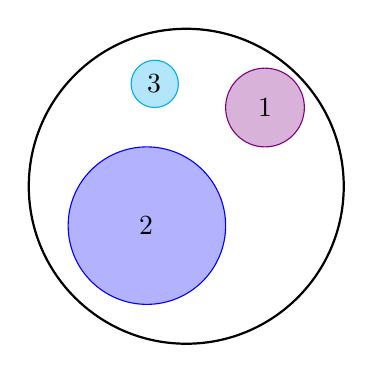
\begin{tikzpicture}[scale=1, transform shape]
            \draw[thick] (0,0) circle [radius=2];
            \filldraw[color=violet,fill=violet!30] (1,1) circle [radius=0.5];
            \node at (1,1) {$1$};
            \filldraw[color=blue,fill=blue!30] (-0.5,-0.5) circle [radius=1];
            \node at (-0.5,-0.5) {$2$};
            \filldraw[color=cyan,fill=cyan!30] (-0.4,1.3) circle [radius=0.3];
            \node at (-0.4,1.3) {$3$};
        \end{tikzpicture}
        \end{center}
        \caption{Morphism in $(\E_2^{\otimes})_{\ms{act}}$.}%
        \label{fig:E2operad}
        \end{figure}
        \item Composition is simply composition of embeddings.
    \end{itemize}
    This category is clearly topologically enriched and has a symmetric monoidal structure given by disjoint union.
\end{defn}

\begin{defn}
    An \textit{$\E_n$-algebra} in a symmetric monoidal $\infty$-category $\mc{C}$ is a symmetric monoidal functor
    \[ (\E_n^{\otimes})_{\ms{act}} \to \mc{C}. \]
    We will denote the $\infty$-category of $\E_n$-algebras in $\mc{C}$ by
    \[ \ms{Alg}_{\E_n}(\mc{C}) \coloneqq \ms{Fun}^{\otimes} ((\E_n^{\otimes})_{\ms{act}}, \mc{C}). \]
\end{defn}

Note that all mapping spaces in $(\E_n^{\otimes})_{\ms{act}}$ are determined by
\[ \ms{Map}_{(\E_n^{\otimes})_{\ms{act}}} (D^n \sqcup \cdots \sqcup D^n, D^n). \]
This has a map
\[ \ms{Map}_{(\E_n^{\otimes})_{\ms{act}}} (D^n \sqcup \cdots \sqcup D^n, D^n) \to \ms{Conf}_k (D^n) \subseteq D^n \]
given by evaluation at the center of each disk. Here, $\ms{Conf}_k(D^n) \subseteq D^n$ is the \textit{configuration space} and is simply the locus where no two points agree.

\begin{exer}
    Prove that the evaluation map we just defined is a homotopy equivalence.
\end{exer}

As an example, it is clear that
\[ \ms{Map}_{(\E_n^{\otimes})_{\ms{act}}} (D^n, D^n) \simeq \ms{Conf}_1 (D^n) \simeq \pt. \]
The next example is
\[ \ms{Map}_{(\E_n^{\otimes})_{\ms{act}}} (D^n \sqcup D^n, D^n) \simeq \ms{Conf}_2 (D^n) \simeq S^{n-1}. \]

Now suppose we have an $\E_n$-algebra $\ul{A} \colon (\E_n^{\otimes})_{\ms{act}} \to \mc{C}$ with underlying algebra $\ul{A}(D^n) = A$. We also have a morphism
\[ S^{n-1} \to \ms{Map}(A \otimes A, A) \]
and other morphisms. Restricting to the $0$-cell, this is a multiplication morphism.

To try to understand $\E_n$-algebras, we may try to begin with $n=1$.
\begin{prop}
    There is an equivalence
    \[ N\ms{Ass}_{\mc{act}}^{\otimes} \to (\E_1^{\otimes})_{\ms{act}} \]
    of symmetric monoidal $\infty$-categories which sends a finite set $S$ to disjoint union $\bigsqcup_S D^1$.
\end{prop}

\begin{proof}
    First, we show that all mapping spaces in $(\E_1^{\otimes})_{\ms{act}}$ are discrete. Up to homotopy, a map $D^1 \sqcup \cdots \sqcup D^1 \to D^1$ is simply an ordering of the indexing set of connected components of the source. This is precisely the set of maps in $\ms{Ass}_{\ms{act}}^{\otimes}$. This functor sends disjoint unions to disjoint unions, and finally a symmetric monoidal functor between symmetric monoidal $\infty$-categories is an equivalence in the $\infty$-category of symmetric monoidal $\infty$-categories if and only if the underlying functor is an equivalence.
\end{proof}

\begin{cor}
    We have an equivalence
    \[ \ms{Alg}_{\E_1}(\mc{C}) \cong \ms{Alg}(\mc{C}). \]
\end{cor}

\begin{exer}
    Figure out what $\E_0$-algebras are in an arbitrary symmetric monoidal $\infty$-category. Next, figure out what $\E_2$-algebras in the $\infty$-category $\ms{Cat}$ of $1$-categories are (you should get braided monoidal categories).
\end{exer}

There are functors
\[ (\E_0^{\otimes})_{\ms{act}} \to (\E_1^{\otimes})_{\ms{act}} \to \cdots \]
given by taking the Cartesian product with $D^1$. These are symmetric monoidal functors, so we have induced functors
\[ \cdots \to \ms{Alg}_{\E_1}(\mc{C}) \to \ms{Alg}_{\E_0}(\mc{C}). \]

\begin{defn}
    The $\infty$-category of \textit{$\E_{\infty}$-a;gebras} is the inverse limit of the diagram
    \[ \cdots \to \ms{Alg}_{\E_1}(\mc{C}) \to \ms{Alg}_{\E_0}(\mc{C}) \]
    in $\ms{Cat}_{\infty}$.
\end{defn}

\begin{thm}
    We have an equivalence
    \[ \ms{Alg}_{\E_{\infty}}(\mc{C}) \cong \ms{CAlg}(\mc{C}). \]
\end{thm}

\begin{proof}[Sketch of proof]
    First, note that
    \begin{align*}
        \ms{Alg}_{\E_{\infty}}(\mc{C}) &\cong \varprojlim \ms{Alg}_{\E_n}(\mc{C}) \\
        &\simeq \varprojlim \ms{Fun}^{\otimes}((\E_n^{\otimes})_{\ms{act}}, \mc{C}) \\
        &\simeq \ms{Fun}^{\otimes} (\colim (\E_n^{\otimes})_{\ms{act}}, \mc{C}).
    \end{align*}
    Proving that this colimit is equivalent to $N \ms{Comm}_{\ms{act}}^{\otimes}$ is left as an exercise.
\end{proof}

We will now state a very important result. The proof is very hard, but the statement should be understandable. Let $(\mc{C}, \otimes)$ be a closed symmetric monoidal category or at least have the property that $-\otimes c$ commutes with filtered colimits and geometric realizations. We will also assume that $\mc{C}$ has all limits and colimits.

\begin{thm}[Lurie]\leavevmode
    \begin{enumerate}
        \item The $\infty$-category $\ms{Alg}_{\E_n}(\mc{C})$ admits all limits and colimits for any $0 \leq n \leq \infty$. The forgetful functor
        \[ \ms{Alg}_{\E_n}(\mc{C}) \to \mc{C} \]
        preserves filtered colimits, geometric realizations, and all limits. Moreover, it detects equivalences.
        \item When $n = \infty$, the coproduct and tensor product coincide.
        \item The $\infty$-category $\ms{Alg}_{\E_n}(\mc{C})$ admits a symmetric monoidal structure such that $\ms{Alg}_{\E_n}(\mc{C}) \to \mc{C}$ is symmetric monoidal.
    \end{enumerate}
\end{thm}

\begin{exer}
    Do the $1$-categorical analogue of the theorem in the category $\ms{Ab}$ of abelian groups.
\end{exer}

We will now discuss $\E_n$-algebras in the $\infty$-category of spaces $\mc{S}$ equipped with symmetric monoidal structure given by the Cartesian product. Then $\ms{Alg}(\mc{S})$ is the category of ``monoids'' in $\mc{S}$. For any such space $X$, the set of connected components $\pi_0(X)$ is a monoid.

\begin{defn}
    We say $X$ is \textit{grouplike} if $\pi_0 (X)$ is a group. This is equivalent to saying that the shear map
    \[ X \times X \to X \times X \qquad (a,b) \mapsto (ab, b) \]
    is a homotopy equivalence. In addition, we say an $\E_n$-algebra is \textit{grouplike} if the underlying $\E_1$-algebra is grouplike.
\end{defn}

For every pointed space $X \in \mc{S}_*$, the iterated loop space
\[ \Omega^n X \simeq \ms{Map}_{\mc{S}_*}(S^n, X) \cong \ms{Map}((D^n, \partial D^n), (X, *)) \]
is canonically an $\E_n$-algebra in $\mc{S}$.

\begin{exer}
    Make this $\E_n$-algebra structure precise by giving a functor $(\E_n^{\otimes})_{\ms{act}} \to \mc{S}$ of topologically enriched categories.
\end{exer}

\begin{thm}[Boardman-Vogt]\label{thm:enalgspaces}
    The functor 
    \[ \Omega^n \colon \mc{S}_*^{n\ms{-conn}} \to \ms{Alg}_{\E_n}(\mc{S}) \]
    is fully faithful with essential image the grouplike $\E_n$-algebras for any $0 \leq n < \infty$.
\end{thm}

\begin{cor}
    For any $\E_n$-algebra $A$ in $\mc{S}$ and any connected pointed space $X \in \mc{S}_*^{\ms{conn}}$, we have that
    \[ \ms{Map}_{\E_n}(\Omega^n \Sigma^n X, A) \cong \ms{Map}_{\mc{S}_*}(X, A). \]
\end{cor}

\begin{proof}
    We can consider the subspace $A' \subseteq A$ consisting of the unit component $\pi_0(A') \subseteq \pi_0(A)$. Then
    \begin{align*}
        \ms{Map}_{\E_n}(\Omega^n \Sigma^n X, A) &\simeq \ms{Map}_{\E_n} (\Omega^n \Sigma^n X, A').
    \end{align*}
    Similarly, we have
    \[ \ms{Map}_{\mc{S}_*}(X, A) \simeq \ms{Map}_{\mc{S}_*}(X, A'). \]
    Therefore, we may assume that $A$ is grouplike. But this means that $A = \Omega^n Y$ for some pointed $n$-connected space $Y$. This implies that
    \begin{align*}
        \ms{Map}_{\E_n}(\Omega^n \Sigma^n X, \Omega^n Y) &\cong \ms{Map}_{\mc{S}_*} (\Sigma^n X, Y) \\
        &\cong \ms{Map}_{\mc{S}_*}(X, \Omega^n Y) \\
        &\cong \ms{Map}_{\mc{S}_*}(X, A). \qedhere
    \end{align*}
\end{proof}

\begin{proof}[Sketch of proof of~\Cref{thm:enalgspaces}]
    We begin with the case of $n=1$. Here, we have the functor
    \[ \Omega \colon \mc{S}_*^{\ms{conn}} \to \ms{Alg}_{\E_1}^{\ms{gp}}(\mc{S}). \]
    We will construct an inverse using the bar construction, which is given by
    \[ \ms{Bar}(G) \coloneqq \colim_{\Delta^{\op}} \ab(\cdots G \times G \triple{\to} G \rightrightarrows \pt). \]
    The result we need is that $\Omega \ms{Bar}(G) \simeq G$ is an equivalence of spaces. This is usually done by constructing a fiber sequence
    \[ G \to EG \to BG. \]

    The general step is now to induct on $n$. For example, if we consider $\mc{S}_*^{2\ms{-conn}}$, its image in $\ms{Alg}_{\E_1}^{\ms{Sp}}(\mc{S}_*^{\ms{conn}})$. Therefore we have a chain
    \begin{equation*}
    \begin{tikzcd}
        \ms{S}_*^{2\ms{-conn}} \ar[shift left=1]{r} & \ms{Alg}_{\E_1}^{\ms{gp}} (S_*^{\ms{conn}})\ar[shift left=1]{r} \ar[shift left=1]{l} & \ms{Alg}_{\E_1}(\ms{Alg}_{\E_1}^{\ms{gp}}(\mc{S})). \ar[shift left=1]{l}
    \end{tikzcd}
    \end{equation*}
    This is actually the same as $\E_2$-algebras, and the general case works the same way and the desired result follows from~\Cref{thm:dunnadditivity}.
\end{proof}

\begin{thm}[Dunn additivity]\label{thm:dunnadditivity}
    For any symmetric monoidal $\infty$-category $\mc{C}$, we have
    \[ \ms{Alg}_{\E_{n+m}}(\mc{C}) \cong \ms{Alg}_{\E_m}(\ms{Alg}_{\E_n}(\mc{C})) \]
    for all $n, m \geq 0$.
\end{thm}

Note that the $1$-categorical version of this is the Eckmann-Hilton argument.

\begin{cor}
    Suppose that $\mc{C}$ has sifted colimits and $\otimes$ commutes with them in both variables separately. Then
    \[ \ms{Bar} \colon \ms{Alg}_{\E_n}(\mc{C})_{/\1} \to \ms{Alg}_{\E_{n-1}}(\mc{C}) \]
    given by 
    \[ A \mapsto \colim \ab(\cdots A \otimes A \triple{\to} A \rightrightarrows \1) \]
    is well-defined.
\end{cor}

\begin{proof}
    Note that it is simply given by
    \[ \ms{Alg}_{\E_n} \cong \ms{Alg}_{\E_1} (\ms{Alg}_{\E_{n-1}}(\mc{C})) \to \ms{Alg}_{\E_1}(\mc{C}). \qedhere \]
\end{proof}

\subsection{$p$-adic completion}%
\label{sub:p-adic completion}

We will generalize the process of going from $\Z$ to $\Z_p$ in the world of spectra. In addition, we will see how spectra can be recovered from their $p$-completions and their rationalizations.

Recall that an abelian group $A$ is \textit{$p$-complete} if it is complete (and separated) with respect to the $p$-adic topology on $A$. This is the topology which has a neighborhood basis of $0$ given by $p^n A \subseteq A$. Equivalently, this says that
\[ A \xrightarrow{\sim} \varprojlim A/p^n \eqqcolon A^{\sw}_p. \]

\begin{defn}
    For a spectrum $X \in \ms{Sp}$ and an integer $n \in \Z$, define $X/n$ to be the cofiber of the map $X \xrightarrow{n} X$ given by the addition of identity morphism $n$ times. Equivalently, we have
    \[ X/n \simeq X \otimes_{\bS} \bS/n. \]
\end{defn}

As we would expect, if $n \mid m$, then there is a canonical map
\[ X/m \to X/n \] defined as the cofiber of
\begin{equation*}
\begin{tikzcd}
    X \ar{d}{m} \ar{r}{m/n} & X \ar{d}{n} \\
    X \ar{r}{\mr{id}} \ar{d} & X \ar{d} \\
    X/m \ar{r} & X/n.
\end{tikzcd}
\end{equation*}

\begin{defn}
    For a spectrum $X \in \ms{Sp}$, we define its \textit{$p$-completion} to be the spectrum
    \[ X_p^{\sw} \coloneqq \varprojlim (\cdots \to X/p^3 \to X/p^2 \to X/p). \]
\end{defn}
Note that there is a canonical map $X \to X_p^{\sw}$ induced from the projections $X \to X/p^n$.

\begin{rmk}
    All of these constructions are well-defined up to contractible choice.
\end{rmk}

\begin{defn}
    A spectrum $X$ is \textit{$p$-complete} if the map $X \to X_p^{\sw}$ is an equivalence. Denote the $\infty$-category of $p$-complete spectra by $\ms{Sp}_p^{\sw}$.
\end{defn}

\begin{thm}\leavevmode
    \begin{enumerate}
        \item For every spectrum $X$, the spectrum $X_p^{\sw}$ is $p$-complete.
        \item The functor $(-)_p^{\sw} \colon \ms{Sp} \to \ms{Sp}_p^{\sw}$ is left adjoint to the inclusion $\ms{Sp}_p^{\sw} \hookrightarrow \ms{Sp}$.
        \item The $\infty$-category $\ms{Sp}_p^{\sw}$ has all limits and colimits.
    \end{enumerate}
\end{thm}

\begin{proof}[Sketch of proof]
    We will first prove that $X_p^{\sw}$ is $p$-complete. First, note that $\ms{Sp}_p^{\sw}$ is closed under limits and finite colimits. This is true because the functor $-/p$ is a cofiber and so commutes with all limits and colimits and the limit functor commutes with limits and finite colimits. The second step is to prove that for any $X$, $X/p$ is $p$-complete. This implies that $X/p^n$ is $p$-complete by using the fiber sequence
    \[ X/p \xrightarrow{p^{n-1}} X/p^n \to X/p^{n-1}. \]
    This implies that $X_p^{\sw}$ is $p$-complete.

    First, note that the functor $(-)_p^{\sw}$ is idempotent. This means that
    \[ (X_p^{\sw})_p^{\sw} \simeq X_p^{\sw}. \]
    If $Y$ is a $p$-complete spectrum, we can construct an inverse to
    \[ \ms{Map}(X, Y) \gets \ms{Map}(X_p^{\sw}, Y) \]
    by applying $p$-completion to everything.

    We know already that limits and finite colimits exist. For an arbitrary colimit of a functor $I \xrightarrow{X} \ms{Sp}_p^{\sw}$, the colimit is simply given by
    \[ \ab(\colim_I^{\ms{Sp}} X_i)_p^{\sw}. \qedhere \]
\end{proof}

\begin{exer}
    Prove that a spectrum $X$ is $p$-complete if and only if
    \[ \lim (\cdots \to X \xrightarrow{p} X \xrightarrow{p} X) \simeq 0. \]
    Moreover, prove that $X/p$ is $p$-complete for any spectrum $X$.
\end{exer}

\begin{defn}
    A map $f \colon X \to Y$ of spectra is a \textit{$p$-adic equivalence} if the induced map
    \[ f_p^{\sw} \colon X_p^{\sw} \to Y_p^{\sw} \]
    is an equivalence.
\end{defn}

Note that if $X$ and $Y$ are $p$-complete, then $f$ is a $p$-adic equivalence if and only if $f$ is an equivalence.

\begin{prop}\leavevmode
    \begin{enumerate}
        \item A map $f \colon X \to Y$ is a $p$-adic equivalence if and only if the map
        \[ f/p \colon X/p \to Y/p \]
        is an equivalence.
        \item A map $f \colon X \to Y$ between connective $X, Y$ is a $p$-adic equivalence if and only if the induced map
        \[ X \otimes_{\bS} H\F_p \to Y \otimes_{\bS} H\F_p \]
        is an equivalence (in other words, we can check equivalence on homology).
    \end{enumerate}
\end{prop}

\begin{proof}
    The proof is left as an exercise to the reader.
\end{proof}

Now we know that $p$-adic equivalences have nice properties, but it is not clear how to tell whether a spectrum is $p$-complete.

\begin{prop}
    Let $A$ be an abelian group. If $A$ is $p$-complete, then so is $HA \in \ms{Sp}$.
\end{prop}

For example, we see that $H \Z_p$ is $p$-complete. The converse unfortunately fails in general, but it does hold if $A$ has bounded order of $p^{\infty}$-torsion.

\begin{defn}
    An abelian group $A$ is \textit{derived $p$-complete} if the Eilenberg-Maclane spectrum $HA$ is $p$-complete.
\end{defn}

\begin{rmk}
    There is also a notion of $p$-completeness in $\mc{D}(\Z)$. Everything works exactly as in $\ms{Sp}$. Then $A$ is derived $p$-complete if and only if it is $p$-complete as an object of $\mc{D}(\Z)$. This is equivalent to the condition that there is a quasi-isomorphism
    \[ A \simeq R\varprojlim \ms{Cone}(A \xrightarrow{p^n} A) \in \mc{D}(\Z). \]
\end{rmk}

\begin{thm}\leavevmode
    \begin{enumerate}
        \item A spectrum $X$ is $p$-complete if and only if $\pi_n (X)$ is derived $p$-complete for all $n$.
        \item Assume that $\pi_n(X)$ has bounded order of $p^{\infty}$-torsion for each $n$. Then
        \[ \pi_* (X_p^{\sw}) = \pi_*(X)_p^{\sw}. \]
    \end{enumerate}
\end{thm}

\begin{exm}
    The most important example of a $p$-complete spectrum is the $p$-adic completion $\bS_p^{\sw}$ of the sphere. We can compute
    \[ \pi_*(\bS_p^{\sw}) = \begin{cases}
        \Z_p & *=0 \\
        \ab\{\text{$p^{\infty}$-torsion in } \pi_*(\bS) \} & > 0 \\
        0 & * < 0.
    \end{cases} \]
    Another example is simply $(H\Q)_p^{\sw} = 0$ because multiplication by $p$ is an isomorphism on $\Q$.
\end{exm}

There are some nice monoidal properties associated to $p$-complete spectra which are listed below. We will not prove these.
\begin{itemize}
    \item The category $\ms{Sp}_p^{\sw}$ of $p$-complete spectra admits a closed symmetric monoidal structure given by
    \[ X \hat{\otimes}_p Y \coloneqq (X \otimes_{\bS} Y)_p^{\sw}. \]
    In particular, the $p$-completion functor is strong symmetric monoidal.
    \item If $R$ is an $\E_n$-algebra, then so is $R_p^{\sw}$ and $R \to R_p^{\sw}$ is an $\E_n$-map exhibiting $R_p^{\sw}$ as the initial $p$-complete $\E_n$-algebra under $R$.
\end{itemize}

It is much easier to deal with $p$-complete spectra than to deal with spectra. However, this is only useful if we can recover spectra from their $p$-completions.

\begin{quest}
    Can we recover any spectrum $X$ from its $p$-completions $X_p^{\sw}$ as $p$ ranges over all primes?
\end{quest}

The answer to this question must be no by the example of $H\Q$. In order to even attempt to have an affirmative answer, we will also need to consider rationalization. Here, recall that an abelian group $A$ is \textit{rational} if it is uniquely divisible. Equivalently, it is a $\Q$-vector space.

\begin{defn}
    A spectrum $X$ is \textit{rational} if $\pi_n (X)$ is rational for each $n$. We denote the full subcategory of rational spectra by $\ms{Sp}_{\Q} \subseteq \ms{Sp}$.
\end{defn}

This is actually even better-behaved than $p$-completeness.
\begin{thm}\leavevmode
    \begin{enumerate}
        \item A spectrum is rational if and only if it admits the structure of an $H\Q$-module.
        \item For any spectrum $X$, the spectrum $X \otimes_{\bS} H\Q \eqqcolon X_{\Q}$ is rational and $\pi_*(X_{\Q}) = \pi_*(X)_{\Q}$. 
        \item The functor $-\otimes_{\bS} H\Q \colon \ms{Sp} \to \ms{Sp}_{\Q}$ is left adjoint to the inclusion $\ms{Sp}_{\Q} \subseteq \ms{Sp}$.
        \item The category $\ms{Sp}_{\Q} \subseteq \ms{Sp}$ is closed under limits and colimits.
        \item We have an equivalence
        \[ \ms{Sp}_{\Q} \cong \ms{Mod}_{H\Q} \simeq \mc{D}(\Q). \]
        \item The category $\ms{Sp}_{\Q}$ is symmetric monoidal with tensor product
        \[ X \otimes_{\bS} Y = X \otimes_{H\Q} Y \]
        and unit $H\Q$.
    \end{enumerate}
\end{thm}

\begin{exer}
    Prove this theorem using the fact that $H\Q \otimes_{\bS} H\Q = H\Q$.
\end{exer}

We can now refine our question.
\begin{quest}
    Can we recover any spectrum $X$ from its $p$-completions $X_p^{\sw}$ as $p$ ranges over all primes together with its rationalization $X_{\Q}$?
\end{quest}

Our slogan will be that the answer to this question is yes if we also include the data of a certain ``gluing map.'' This uses something known as the Hasse square.

For every spectrum we have maps
\[ X \to X_p^{\sw} \qquad \text{and} \qquad X \to X_{\Q}. \]
In addition, rationalizing the $p$-completion map, we have maps
\[ X_{\Q} \to (X_p^{\sw})_{\Q} \eqqcolon X_{\Q_p}. \]
By naturality properties of rationalization, we obtain a commutative square
\begin{equation*}
\begin{tikzcd}
    X \ar{r} \ar{d} & \prod_p X_p^{\sw} \ar{d} \\
    X_{\Q} \ar{r} & \ab(\prod_p X_{p}^{\sw})_{\Q}.
\end{tikzcd}
\end{equation*}
This is called the \textit{Hasse square} or the \textit{fracture square}.

\begin{thm}
    For any spectrum $X$, this square is a fiber product.
\end{thm}

This theorem is proved by noting that $p$ is invertible on the fiber of $X \to X_p^{\sw}$. Therefore, the fiber of the top row is rational (because all primes are invertible), so it equals its rationalization, which is the fiber of the bottom row.

The theorem can be refined to the categorical level. In particular, we have a pullback diagram
\begin{equation*}
\begin{tikzcd}
    \ms{Sp} \ar{r}{\prod_p (-)_p^{\sw}} \ar{d}[swap]{X_{\Q} \to \ab(\prod_p X_p^{\sw})_{\Q}} & \prod_p \ms{Sp}_p^{\sw} \ar{d}{(X_p)_p \mapsto \ab(\prod_p X_p)_{\Q}} \\
    \ms{Sp}_{\Q}^{\Delta^1} \ar{r}{\mr{target}} & \ms{Sp}_{\Q}
\end{tikzcd}
\end{equation*}
of $\infty$-categories. This means that we can decompose the entire $\infty$-category of spectra.

Unfortunately, this morphism is not symmetric monoidal, but it at least behaves well with respect to $\E_n$-algebras. More precisely, there is a pullback square
\begin{equation*}
\begin{tikzcd}
    \ms{Alg}_{\E_n}(\ms{Sp}) \ar{r} \ar{d} & \prod_p \ms{Alg}_{\E_n}(\ms{Sp}_p^{\sw}) \ar{d} \\
    (\ms{Alg}_{\E_n}(\ms{Sp}_{\Q}))^{\Delta^1} \ar{r} & \ms{Alg}_{\E_n}(\ms{Sp}_{\Q})
\end{tikzcd}
\end{equation*}
of $\infty$-categories, where the arrows are given by restriction from the previous square.


\subsection{Tate construction}%
\label{sub:Tate construction}

Let $G$ be a group object in $\mc{S}$. In particular, this means that $G$ is a group-like $\E_1$-space. These can in fact be modeled by topological groups, but the correct generality is that of group-like $\E_1$-spaces. There is a classifying space $BG \in \mc{S}$ given by the bar construction. If $\mc{C}$ is any $\infty$-category, we will let
\[ \mc{C}^{BG} = \ms{Fun}(BG, \mc{C}) \]
denote the category of objects in $\mc{C}$ with a $G$-action.

\begin{con}
    We will consider $G$ as an object in $\mc{S}^{G \times G}$ by letting $G \times G$ act on $G$ by the action 
    \[ (g,h) \cdot h \coloneqq gxh^{-1}. \]
\end{con}

\begin{defn}[Klein]
    We define a spectrum $D_G \in \ms{Sp}^{BG}$ called the \textit{dualizing spectrum} of $G$ as
    \[ D_G \coloneqq (\Sigma_+^{\infty} G)^{h(G \times 1)} \]
    with its remaining $G = 1 \times G$-action.
\end{defn}

The name dualizing spectrum needs a justification, which will be given in the remainder of this section. Before we do this, we give some examples.

\begin{exm}
    Assume $G$ is a finite group. Then
    \[ \Sigma_+^{\infty} G = \bigoplus_{g \in G} \bS. \]
    Computing the homotopy fixed points, we obtain
    \[ (\Sigma_+^{\infty} G)^{hG} = \ab(\bigoplus_{g \in G} \bS)^{hG} \simeq \bS. \]
    More precisely, the map
    \[ \ab(\bigoplus_{g \in G} \bS)^{hG} \to \bigoplus_{g \in G} \bS \to \bS \]
    is an equivalence.

    To see this, consider the homotopy fixed point spectral sequence
    \[ H^* \ab(G, \bigoplus_{g \in G} \pi_* \bS) \implies \pi_* \ab(\ab(\bigoplus_{g \in G} \bS)^{hG}). \]
    It is a classical result that
    \[ H^*\ab(G, \bigoplus_{g \in G} A) = \begin{cases}
        A & *=0 \\
        0 & * \neq 0
    \end{cases}. \]
    Therefore the spectral sequence degenerates and yields the result. This implies that $D_G = \bS$ with the trivial action.
\end{exm}

Now suppose that $G$ is a compact Lie group.
\begin{thm}
    If $G$ is a compact Lie group, then
    \[ D_G = \bS^{\g} \coloneqq \Sigma^{\infty}(\g^+) \]
    where $G$ acts by the adjoint representation.
\end{thm}

For example, let $\T = U(1) = S^1$. Then because the adjoint representation of an abelian group is trivial, we have $D_{\T} = \bS^1$ with the trivial action.

Now assume that $BG \simeq (M, m_0)$ for some closed smooth manifold $M$. For example, if $G = \Z$, then $BG \simeq S^1$. Alternatively, we can consider any closed manifold $(M, m_0)$ and let $G = \Omega M$.

\begin{thm}[Atiyah duality]
    The dualizing spectrum is given by
    \[ D_G = \bS^{-T_{m_0} M} \simeq \bS^{-\dim M}, \]
    where we extend the construction $\bS^V$ for any representation of $G$ to a virtual representation. As a functor
    \[ BG \simeq M \to \ms{Sp}, \]
    it sends 
    \[ m \mapsto \bS^{-T_m M}. \]
\end{thm}

\begin{rmk}
    For any space $X$ (in place of $BG$), we can define a dualizing spectrum
    \[ D_X \colon X \to \ms{Sp}. \]
    For example, we can define this functor on connected components because
    \[ X \simeq \bigsqcup B G_i. \]
    In particular, we assign $D_{G_i}$ to $BG_i$.
\end{rmk}

\begin{con}
    Let $\mc{C}$ be a stable $\infty$-category which has all limits and colimits. For any $E \in \ms{Sp}$ and $X \in \mc{C}$, there is an object
    \[ E \otimes X \in \mc{C} \]
    defined such that the functor
    \[ - \otimes X \colon \ms{Sp} \to \mc{C} \]
    preserves colimits and the composite
    \[ \mc{S} \xrightarrow{\Sigma_+^{\infty}} \ms{Sp} \xrightarrow{- \otimes X} \mc{C} \]
    is given by the functor
    \[ M \mapsto M \otimes X = \colim_M c_X. \]
\end{con}

\begin{defn}
    Let $G \in \ms{Alg}_{\E_1}^{\ms{gp}} (\mc{S})$ and $X \in \mc{}^{BG}$. We define the \textit{norm map}
    \[ \mr{Nm}_G \colon (D_G \otimes_{\bS} X)_{hG} \to X^{hG} \]
    as the composite
    \begin{equation*}
    \begin{tikzcd}
        ((\Sigma_+^{\infty} G)^{h(G\times 1)} \otimes_{\bS} X)_{h(1 \times G)} \ar{d} \\
        ((\Sigma_+^{\infty} G \otimes_{\bS} X)^{h(G \times 1)})_{h(1 \times G)} \ar{d} \\
        ((\Sigma_+^{\infty} G \otimes_{\bS} X)_{h(1 \times G)})^{h(G \times 1)} \ar{r}{\sim} & X^{hG}.
    \end{tikzcd}
    \end{equation*}
\end{defn}

\begin{exer}
    Prove that
    \[ ((\Sigma_+^{\infty} G \otimes_{\bS} X)_{h(1 \times G)})^{h(G \times 1)} \simeq X^{hG}. \]
\end{exer}

This is quite an abstract construction, so we will try to get our hands on it with some examples.

\begin{exm}
    If $G$ is finite and $X \in \mc{C}^{BG}$, then the norm map is
    \[ (D_G \otimes X)_{hG} \simeq X_{hG} \to X^{hG}. \]
    For example, if $\mc{C} = \ms{Sp}$ and $X = HM$ for an abelian group $M$ with a $G$-action, then this map is a map
    \begin{equation*}
    \begin{tikzcd}
        HM_{HG} \ar{r}{\mr{nM}} \ar{d} & HM^{hG} \\
        H M_G \ar{r} & H M^G \ar{u}
    \end{tikzcd}
    \end{equation*}
    and is induced from the classical norm map
    \[ M_G \to M^G \qquad [m], \mapsto \sum_{g \in G} gm \]
    from coinvariants to invariants.
    This follows from the fact that for a general $X$, the composite
    \[ X \to X_{hG} \xrightarrow{\mr{Nm}_G} X^{hG} \to X \]
    is the sum over all $g \in G$ of the maps $\rho_g \colon X \to X$ given by multiplication by $g$.
\end{exm}

\begin{exer}
    Prove that if $G$ is finite, the composite
    \[ X \to X_{hG} \xrightarrow{\mr{Nm}_G} X^{hG} \to X \]
    agrees with the map
    \[ \sum_{g \in G} \rho_g \colon X \to X. \]
\end{exer}

\begin{exm}
    When $G = \T$, we get a map
    \[ \Sigma X_{h\T} = (D_{\T} \otimes X)_{h\T} \to X^{h\T}. \]
\end{exm}

\begin{thm}
    The norm map $(D_G \otimes X)_{hG} \to X^{hG}$ is an equivalence provided that one of the following conditions holds:
    \begin{enumerate}
        \item $BG$ is a finite CW complex;
        \item $X$ is induced, which means that $X \simeq \Sigma_+^{\infty} G \otimes Y$ where $G$ acts only on $\Sigma_+^{\infty} G$.
    \end{enumerate}
\end{thm}

\begin{proof}[Sketch of proof]
    In the first case, all limits in the interchange maps are finite. Because all functors in the composite are exact, we are done.

    In the second case, the limits and colimits are still close enough to being finite, so we are done.
\end{proof}

\begin{exm}
    Let $BG$ be a closed manifold $M$, $\mc{C} = \ms{Sp}$, and $X = H\Z$ with the trivial action of $G$. In this case, the norm is a map
    \[ (DG \otimes X)_{hG} \xrightarrow{\sim} X^{hG} = H\Z^{BG}. \]
    The target has homotopy groups given by
    \[ \pi_* (H\Z^{BG}) = H^{-*}(M, \Z). \]
    The source is explicitly given by
    \[ (DG \otimes X)_{hG} \cong (\bS^{-tM} \otimes H\Z)_{hG} \simeq (H\Z[-n])_{hG}, \]
    where $G$ acts on $HZ[-n]$ non-trivially. This has homotopy groups
    \[ \pi_*((H\Z[-n])_{hG}) = H_{*+n}(M, \Z^{w_1}) \]
    given by homology with coefficients in the orientation cover. On homotopy groups, this map
    \[ H_{*+n}(M, \Z^{w_1}) \xrightarrow{\sim} H^{-*}(M, \Z) \]
    is simply Poincar\'e duality (at least if $M$ is orientable).
\end{exm}

If we replace $H\Z$ by any spectrum, we get Poincar\'e duality in arbitrary cohomology theories. If $X = BG$ is a finite CW complex, the norm equivalence is a generalized version of Poincar\'e duality
\[ H_*(X, D_X) \to H^{-*}(X). \]
This can be thought of as being analogous to Serre or Verdier duality in algebraic geometry. If $D_X$ is a parameterized sphere ($D_X = \bS[n]$ as underlying spectra), then this is equivalent to $X$ being a Poincar\'e duality space.

\begin{thm}[Klein]
    The natural transformation (called the \textit{assembly map})
    \[ (D_G \otimes -)_{hG} \to (-)^{hG} \]
    exhibits the functor $(D_G \otimes -)_{hG}$ as the universal functor over $(-)^{hG}$ which preserves colimits.
\end{thm}

Note that this uniquely determines the spectrum $D_G$ as an object of $\ms{Sp}^{BG}$.

\begin{defn}
    For an object $X \in \mc{C}^{BG}$, we define the \textit{Tate object} as the cofiber
    \[ X^{tG} \coloneqq \ms{cofib}(\mr{Nm}_G). \]
\end{defn}

\begin{exm}
    If $BG$ is finite, then $X^{tG} = 0$ for all $X$. If $G$ is finite and $X = HM$ for an abelian group $M$ with a $G$-action, then $(HM)^{tG}$ has homotopy groups given by the Tate cohomology
    \[ \pi_* ((HM)^{tG}) = \hat{H}^{-*}(G, M) \]
    of $G$ with coefficients in $M$.
\end{exm}

\begin{exer}
    Work out what Tate cohomology is in terms of usual homology and cohomology.
\end{exer}

\begin{exm}
    Suppose that $\mc{C}$ is a symmetric monoidal $\infty$-category such that the tensor product commutes with colimits in both variables separately. Then the functor
    \[ (-)^{tG} \colon \mc{C}^{BG} \to \mc{C} \]
    admits a (unique) lax symmetric monoidal structure such that the natural transformation
    \[ (-)^{hG} \to (-)^{tG} \]
    admits a refinement to a symmetric monoidal transformation.
\end{exm}

\begin{cor}
    If $A \in \ms{Alg}_{\E_n}(\mc{C}^{BG}) \simeq \ms{Alg}_{\E_n}(\mc{C})^{BG}$, then $A^{hG} \to A^{tG}$ is a morphism of $\E_n$-algebras.
\end{cor}

\subsection{Tate diagonal}%
\label{sub:Tate diagonal}

The Tate diagonal is a surprising feature of the world of spectra. Before we discuss it, we will motivate it by discussing abelian groups.

Let $A$ be an abelian group. If we try to write a map of sets
\[ A \to A \otimes A, \qquad x \mapsto x\otimes x, \]
this is not a homomorphism. For example, note that
\[ (x+y) \otimes (x+y) = x \otimes x + y \otimes y + (x\otimes y + y \otimes x). \]
Recall now that if $C_p$ is the cyclic group with $p$ elements, there is a norm map
\[ N \colon (A^{\otimes p})_{C_p} \to (A^{\otimes p})^{C_p}, \qquad x_1 \otimes \cdots x_p \mapsto \sum_{\sigma \in C_p} x_{\sigma(1)} \otimes \cdots \otimes x_{\sigma(p)}. \]
Note here that the error term of the map $x \mapsto x \otimes x$ is in the image of the norm map. Therefore, the ``diagonal'' $x \mapsto x \otimes \cdots \otimes x$ induces a homormorphism
\[ A \to (A^{\otimes p})^{C_p}/N((A^{\otimes p})_{C_p}). \]
This homomorphism in fact exhibits
\[ (A^{\otimes p})^{C_p} / N((A^{\otimes p})_{C_p}) \cong A/p. \]

\begin{exer}\leavevmode
    \begin{enumerate}
        \item Prove that $x \mapsto x^{\otimes p}$ induces a homomorphism
        \[ A \to (A^{\otimes p})^{C_p}/N((A^{\otimes p})_{C_p}). \]
        \item Prove that this homomorphism factors through an isomorphism
        \[ A/p \xrightarrow{\sim} (A^{\otimes p})^{C_p}/N((A^{\otimes p})_{C_p}). \]
    \end{enumerate}
\end{exer}

We will now discuss the analogous construction for spectra.
\begin{thm}
    There is a unique lax symmetric monoidal natural transformation
    \[ X \to (X^{\otimes p})^{t C_p}. \]
\end{thm}

In the rest of this section, we will attempt to see where this comes from and understand some of its properties.

\begin{lem}
    The Singer construction
    \[ X \mapsto (X^{\otimes p})^{t C_p} \]
    is an exact functor.
\end{lem}
This result is particularly surprising because the $p$-th tensor power functor is not even additive.

\begin{proof}
    First, suppose $Y \simeq X \oplus Z$. By the binomial theorem, we have
    \begin{align*}
        (X \oplus Z)^{\otimes p} &= X^{\otimes p} \oplus Z^{\otimes p} \oplus \bigoplus_p (X^{\otimes (p-1)} \otimes Z) \oplus \bigoplus_{\binom{p}{2}} (X^{\otimes (p-2)} \otimes Z^{\otimes 2})\oplus \cdots
    \end{align*}
    On all of the non-pure terms, the action of $C_p$ on the connected components is free, so these terms are all induced modules over $C_p$. These terms vanish after taking Tate fixed points.

    In general, consider a cofiber sequence $X \to Y \to Z$ as a ``two-stage filtration'' on $Y$ of the form
    \begin{equation*}
    \begin{tikzcd}
        \cdots \ar{r} & 0 \ar{r} \ar{d} & X \ar{r} \ar{d} & Y \ar{d} \\
        &  0 & X & Z,
    \end{tikzcd}
    \end{equation*}
    where $Z$ appears as the associated graded term. We then obtain a filtration on $Y^{\otimes p}$ of the form
    \[ X^{\otimes p} \to \bigoplus X^{\otimes (p-1)} \otimes Y \to \cdots \to \bigoplus X \otimes Y^{\otimes (p-1)} \to Y^{\otimes p}. \]
    There is a monoidal structure on filtered objects called the \textit{Day convolution structure} which produces this diagram from our filtered object. The associated graded terms are given by
    \[ X^{\otimes p}, \ldots, \bigoplus_p X \otimes Z^{\otimes (p-1)}, Z^{\otimes p}. \]
    Applying Tate fixed points, the associated graded terms are now of the form
    \[ (X^{\otimes p})^{tC_p}, 0, \ldots, 0, (Z^{\otimes p})^{t C_p}. \]
    This implies that we have a cofiber sequence
    \[ (X^{\otimes p})^{t C_p} \to (Y^{\otimes p})^{t C_p} \to (Z^{\otimes p})^{t C_p}. \qedhere \]
\end{proof}

\begin{rmk}
    The Singer construction commutes with suspension as
    \[ ((\Sigma X)^{\otimes p})^{t C_p} \simeq \Sigma (X^{\otimes p})^{t C_p}. \]
    We can write
    \[ (\Sigma X)^{\otimes p} \simeq \bS^p \otimes X^{\otimes p}, \]
    but the action of $C_p$ involves a nontrivial action on $\bS^p$, where we take the suspension spectrum of the one-point compactification of the regular representation of $C_p$. In fact, we have $(\bS^p)^{t C_p} \simeq (\bS^1)^{t C_p}$, where $S^1$ has the trivial action.
\end{rmk}

\begin{lem}[Stable Yoneda Lemma]
    Let $\mc{C}$ be a stable $\infty$-category. We consider the stable $\infty$-category $\ms{Fun}^{\ms{ex}}(\mc{C}, \ms{Sp})$ of exact functors to $\ms{Sp}$. Taking mapping spectra, there exists a natural equivalence
    \[ \ms{map}_{\ms{Fun}^{\ms{ex}}(\mc{C}, \ms{Sp})} (\ms{map}(X, -), F) \simeq F(X). \]
\end{lem}

\begin{proof}[Proof sketch]
    We will reduce this to the $1$-categorical Yoneda lemma. A natural transformation $\ms{Map}(X, -) \to F$ is simply a sequence of natural transformations on the $n$-th underlying spaces with some compatibility conditions. More precisely, we have natural transformations
    \[ \ms{map}(\Sigma^{-n} X, -) \to \Omega^{\infty} \Sigma^n F(-), \]
    which by the ordinary Yoneda lemma yields a sequence of points in 
    \[ \Omega^{\infty} \Sigma^n F(\Sigma^{-n} X)  \simeq \Omega^{\infty} F(X). \]
    In other words, we have an equivalence of spaces
    \[ \ms{Map}_{\ms{Fun}^{\ms{ex}}(\mc{C}, \ms{Sp})} (\ms{map}(X, -), F) \simeq \Omega^{\infty} F(X). \qedhere \]
\end{proof}

Natural transformations $X \to (X^{\otimes p})^{t C_p}$ correspond to maps $\bS \to (\bS^{\otimes p})^{t C_p} \simeq \bS^{t C_p}$. There is a natural choice of map like this given by
\[ \bS \simeq \ms{map}(\Sigma_+^{\infty} \pt, \bS) \to \bS^{h C_p} \simeq \ms{map}(\Sigma_+^{\infty} C_p, \bS) \to \bS^{t C_p}. \]
Note that there are other maps $\bS \to \bS^{t C_p}$, for example the zero map. However, we need a map which preserves the lax symmetric monoidal structure, and the unique such map is the one we have just given.

\begin{lem}
    The functor $\ms{map}(\bS, -)$ is initial among all lax symmetric monoidal exact functors $\ms{Sp} \to \ms{Sp}$.
\end{lem}

We are now ready to discuss some properties of the Tate diagonal. In particular, we will not prove anything.

\begin{thm}
    For a bounded below $X$, the morphism
    \[ X \to (X^{\otimes p})^{t C_p} \]
    exhibits $(X^{\otimes p})^{t C_p}$ as $X_p^{\sw}$. In particular, $(X^{\otimes p})^{t C_p}$ is bounded below.
\end{thm}

In particular, we see that $\bS^{t C_p} \simeq \bS_p^{\sw}$. This is completely different from Tate cohomology for abelian groups and is a special form of the Segal conjecture. Proofs of these results rely on the Adams spectral sequence because the Tate spectral sequences is too messy.

The Tate construction also allows us to define a version of Frobenius on $\E_{\infty}$-ring spectra.
\begin{defn}
    For an $\E_{\infty}$-ring spectrum $R$, we have the \textit{Tate-valued Frobenius}
    \[ R \xrightarrow{\Delta} (R^{\otimes p})^{t C_p} \xrightarrow{\mu^{t C_p}} R^{t C_p} \]
    using the fact that multiplication $R^{\otimes p} \to R$ is equivariant. This follows from the fact that a morphism $(R^{\otimes p})_{h C_p} \to R$ is encoded in the definition of an $\E_{\infty}$-algebra.
\end{defn}

We should think about this as an analogue of the morphism
\[ R \to R/p, \qquad x \mapsto x^p \]
for an ordinary commutative ring $R$.

\begin{exer}
    Prove that it is necessary that $R$ is commutative and that the target is reduced by $p$. Also prove that $x \mapsto x^p$ is a ring homomorphism $R \to R/p$.
\end{exer}

Applying the Tate-valued Frobenius to
\[ \ms{map}(\Sigma_+^{\infty} X, E) \]
for some space $X$ and $\E_{\infty}$-algebra $E$, we obtain \textit{power operations}. For example, Steenrod operations and Adams operations arise in this way.



\chapter{(Topological) cyclic homology}\thispagestyle{firstpage}
\section{Classical Hochschild and cyclic homology}%
\label{sec:Classical Hochschild and cyclic homology}

In this section, we discuss Hochschild homology, (negative, periodic) cyclic homology, the HKR theorem, and related topics.

\subsection{Hochschild homology}%
\label{sub:Hochschild homology}

Let \(k\) be a field and \(R\) be a \(k\)- algebra.

\begin{defn}
    The \textit{Hochschild homology} of \(R\) is the homology of the complex
    \[
        \HH(R/k) \coloneqq (\cdots \xrightarrow{\partial} R \otimes_k R \xrightarrow{\partial} R),
    \]
    where the differential is given by
    \begin{align*}
        \partial(a_0 \otimes \cdots \otimes a_n) \coloneqq{} & a_0 a_1 \otimes \cdots \otimes a_n \\
        &- a_0 \otimes a_1 a_2 \otimes \cdots \otimes a_n \\
        & \cdots \\
        &+ (-1)^n a_n a_0 \otimes \cdots \otimes a_{n-1}.
    \end{align*}
\end{defn}

\begin{rmk}
    This seems related to what happens when you multiply elements placed on an \(S^1\) as in~\Cref{fig:hhcircle}. In fact, we will see later that there is a connection to the actual \(S^1\).
    \begin{figure}[htpb]
    \begin{center}
    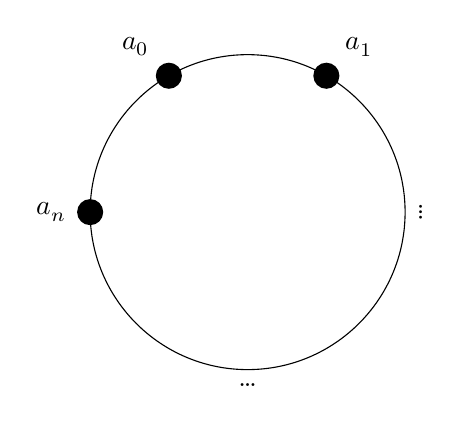
\begin{tikzpicture}[scale=1, transform shape]
        \draw (0,0) circle (2);
        \node[label={north west:{$a_0$}}, fill=black, circle] at (120:2) {};
        \node[label={north east:{$a_1$}}, fill=black, circle] at (60:2) {};
        \node[label={west:{$a_n$}}, fill=black, circle] at (180:2) {};
        \node[rotate=90] at (2.2,0) {\dots};
        \node at (0,-2.2) {\dots};
    \end{tikzpicture}
    \end{center}
    \caption{Components of a basic tensor placed along a circle.}%
    \label{fig:hhcircle}
    \end{figure}
\end{rmk}

\begin{exm}
    For now, set \(R=k\). In this case, we have
    \begin{align*}
        \HH(k/k) &= (\cdots \to k \to k),
    \end{align*}
    where the differentials are alternating sums of $1$ and $-1$. In fact, we see that the complex is
    \[ \HH(k/k) = (\cdots \xrightarrow{0} k \xrightarrow{\mr{id}} k \xrightarrow{0}k), \]
    and therefore the Hochschild homology is
    \[ \HH_*(k/k) = \begin{cases}
        k & *=0 \\
        0 & \text{otherwise}.
    \end{cases} \]
\end{exm}

\begin{exm}
    Because the last differential is given by $a \otimes b \mapsto ab - ba$, we see that
    \[ \HH_0(R/k) = R/[R,R]. \]
    In particular, if $R$ is commutative, we have
    \[ \HH_0(R/k) = R. \]
    In this case, we have
    \[ \HH_1(R/k) = \frac {R \otimes_k R}{\Im \partial} \cong \Omega^1_{R/k}. \]
\end{exm}

We will now recall the definition of the module of K\"ahler differentials.
\begin{defn}
    The \textit{module of K\"ahler differentials} of a commutative ring $R$ is the module $\Omega^1_{R/k}$ generated by $\d{x}$ for all $x \in R$ subject to the following relations:
    \begin{enumerate}
        \item For all $x, y \in R$, we have $\d{(x+y)} = \d{x} + \d{y}$;
        \item For all $x,y \in R$, we have $\d{(xy)} = x \d{y} + y \d{x}$;
        \item For all $x \in k$, we have $\d{x} = 0$.
    \end{enumerate}
    Therefore, we see that $\Omega^1_{R/k}$ receives a universal $k$-linear derivation from $R$.
\end{defn}

There is at most one map
\[ \HH_1(R/k) \to \Omega^1_{R/k} \qquad x \otimes y \mapsto x \cdot \d{y}. \]
\begin{exer}
    Check that this is an isomorphism.
\end{exer}

We will now prove some more properties of Hochschild homology.
\begin{lem}
    If $R$ is commutative, then \(\HH_*(R)\) has the structure of a strictly graded-commutative ring. Here, this means that \(x^2 = 0\) for any \(x\) of odd degree, which is only relevant in characterisic $2$.
\end{lem}

\begin{proof}
    The Hochschild complex $\HH(R/k)$ in fact comes from a simplicial commutative ring
    \begin{equation*}
    \begin{tikzcd}
        \cdots \ar[r,altstackar=7] & R \otimes_k \otimes_k R \ar[r,altstackar=5] & R\otimes_k R \ar[r,altstackar=3] & R,
    \end{tikzcd}
    \end{equation*}
    where the face maps are the components of the differential $\partial$. The desired result then follows by~\Cref{thm:eilenbergzilber}.
\end{proof}

On the de Rham side, there is also a multiplicative structure.
\begin{defn}
    The \textit{de Rham complex} is the exterior algebra
    \begin{align*}
        \Omega^*_{R/k} &\coloneqq \Lambda_R^* \Omega^1_{R/k} \\
        &= \bigoplus_{k \geq 0} \Lambda_R^k \Omega^1_{R/k} \\
        &= \frac{\Sym_R \Omega^1_{R/k}[1]}{x^2 = 0, x \in \Omega^1_{R/k}}.
    \end{align*}
\end{defn}

By extending from degree $1$, we obtain a map $\Omega^*_{R/k} \to \HH_*(R/k)$.

\begin{thm}[Hochschild-Kostant-Rosenberg]\label{thm:hkr}
    If $R/k$ has cotangent complex concentrated in degree $0$, then the map
    \[ \Omega^*_{R/k} \to \HH_*(R/k) \]
    is an isomorphism.
\end{thm}

We will discuss the cotangnet complex later, but for now we may think that $R$ is a smooth or ind-smooth $k$-algebra.

\begin{rmk}
    The differential on $\Omega^*_{R/k}$ does not play a role here. Studying what it corresponds to on the Hochschild side will leade us to cyclic homology.
\end{rmk}

\begin{exer}
    Find an explicit description of $\Omega^*_{k[x_1, \ldots, x_n]/k}$ and in particular show that it is concentrated in degrees at most $n$.
\end{exer}

We will now extend to the case when $k$ is an arbitrary commutative ring. This will lead to flatness issues, so we will fix this by taking derived tensor products. For now, we will let $R$ be a dg-algebra over $k$ which is $K$-flat. This is a flatness condition, but when $R$ is bounded below, it agrees with levelwise flatness. Over $\Z$, it always agrees with levelwise flatness. For such an $R$, we define the Hochschild complex by
\[ \HH(R/k) \coloneqq \Tot(\cdots \to R \otimes_k R \to R). \]
If $R$ is not $K$-flat, we will simply replace it by a $K$-flat resolution $R^{\flat}$ and define
\[ \HH(R/k) \coloneqq \HH(R^{\flat}.k). \]
This is well-defined up to quasi-isomorphism.

\begin{prop}
    For a dg-algebra $R$, there is a quasi-isomorphism
    \[ \HH(R/k) \simeq R \otimes_{R \otimes_k^{\L} R^{\mr{op}}}^{\L} R. \]
\end{prop}

\begin{rmk}
    This is usually called Shukla homology, but we will not make this distinction here.
\end{rmk}

\begin{proof}
    Replacing $R$ by a flat resolution, we consider the complex
    \[ \Tot(\cdots \to R \otimes_k R \otimes_k R \to R \otimes_k R) \simeq R. \]
    The differentials are given by multiplying adjacent terms, but without the $a_n a_0$ term (think configurations on an interval). This complex is usually called the \textit{bar complex}. Applying $- \otimes_{R \otimes_k R^{\op}} R$, the resulting total complex computes the desired complex $R \otimes_{R \otimes_k R^{\op}}^{\L} R$, but it also computes $\HH_*(R/k)$.
\end{proof}

\begin{lem}
    If $R$ is a dg-algebra which arises from a simplicial commutative $k$-algebra, then $\HH(R/k)$ also comes from a simplicial commutative $k$-algebra. In particular, the Hochschild homology groups $\HH_*(R/k)$ form a strictly graded-commutative $k$-algebra.
\end{lem}

\begin{proof}
    We replace $R$ by a flat simplicial commutative $k$-algebra. Then $\HH(R_n/k)$ gives a \textbf{bisimplicial} commutative $k$-algebra. The total complex is then quasi-isomorphic to the diagonal, which is clearly simplicial.
\end{proof}

\begin{lem}
    If $A, B$ are dg-algebras, then
    \[ \HH(A \otimes^{\L} B/k) \simeq \HH(A/k) \otimes_k^{\L} \HH(B/k). \]
\end{lem}

\begin{rmk}
    If $R$ is commutative, then setting $A=B=R$ gives a multiplication map on $\HH$ via the multiplication of $R$.
\end{rmk}

\begin{proof}
    Because $\HH(A/k)$ and $\HH(B/k)$ are simplicial dg-algebras, the tensor product
    \[ \HH(A/k) \otimes_k^{\L} \HH(B/k) \]
    is a bisimplicial dg-algebra. Taking the total complex in all three directions, the result is quasi-isomorphic to the diagonal, which is precisely
    \[ \HH(A\otimes_k^{\L} B). \qedhere \]
\end{proof}

We are now ready to prove the HKR theorem for polynomial rings. As we will see later, we will reduce the general case to this one.
\begin{proof}[Proof of~\Cref{thm:hkr} for polynomial rings]
    In the case of $R = k[x]$, we have
    \[ \Omega^*_{k[x]/k} = k[x] \otimes \Lambda(\d{x}). \]
    Then we only need to check that $\HH(k[x]/k)$ vanishes in degree greater than $1$. This is given by
    \begin{align*}
        \HH(k[x]/k) &= k[x] \otimes^{\L}_{k[x] \otimes_k k[x]} k[x] \\
        &= k[x] \otimes_{k[a,b]}^{\L} k[x].
    \end{align*}
    We have the resolution
    \[ k[a,b] \xrightarrow{\cdot (a-b)} k[a,b] \]
    of $k[x]$, and this gives the desired result.

    For \(R = k[x_1, \ldots, x_n]\) This is simply a tensor product
    \[ R = k[x_1] \otimes_k \cdots \otimes_k k[x_n], \]
    so because both sides of the HKR theorem commute with tensor products, we obtain the desired result.

    Finally, if \(R = k[x_i \mid i \in I]\), we write \(R\) as a filtered colimit of finitely-generated polynomial algebras by writing the set $\ab\{x_i \mid i \in I\}$ of generators as a filtered colimit of its finite subsets. Because both sides commute with filtered colimits, we are done.
\end{proof}

We will now turn to an extremely non-smooth example.
\begin{prop}
    We have
    \[ \HH_*(\F_p/\Z) = \F_p \ab<x>, \]
    where the $\ab<x>$ means the free divided power algebra generated by $x$.
\end{prop}

\begin{proof}
    We will compute the derived tensor product
    \[ \F_p \otimes_{\F_p \otimes^{\L} \F_p} \F_p. \]
    We will resolve $\F_p$ by the dg-algebra
    \[ \Z[\ep]/\ep^2, \qquad \partial \ep = p, \qquad \ab|\ep| = 1. \]
    The tensor product is then given by
    \[ A \simeq \F_p \otimes^{\L} \F_p \simeq \F_p[\ep]/\ep^2. \]
    We will resolve $\F_p$ as an $A$-algebra by
    \[ A\ab<x> = \frac{A[x_1, x_2, \ldots]}{x_ix_j = \binom{i+j}{i} x_{i+j}}, \qquad \partial x_i = \ep x_{i-1}, \qquad \ab|x_i| = 2i, \]
    and the desired result follows by taking the tensor product.
\end{proof}

\subsection{The Connes operator}%
\label{sub:The Connes operator}

We will describe an operator on $\HH$ which corresponds to the de Rham differential. Recall that the de Rham differential
\[ \d \colon \Omega^*_{R/k} \to \Omega^{*+1}_{R/k} \]
is induced from the universial derivation $\d \colon R \to \Omega^1_{R/k}$ by the Leibniz rule.

\begin{defn}
    Let $R$ be an associative $k$-algebra. We define a $k$-linear map
    \[ B \colon \HH(R/k)_n \to \HH(R/k)_{n+1} \]
    by the formula
    \[ r_0 \otimes \cdots \otimes r_n \mapsto \sum_{\sigma \in C_{n+1}} (-1)^{n\sigma(0)} (1 \otimes r_{\sigma} + (-1)^n r_{\sigma} \otimes 1), \]
    where we define
    \[ r_{\sigma} \coloneqq r_{\sigma(0)} \otimes \cdots \otimes r_{\sigma(n)}. \]
\end{defn}
This formula is related to the \textit{cyclic objects} introduced by Connes, and there is a way to think about it systematically in the topological setting, which we will discuss later.

\begin{exer}
    Check that
    \begin{enumerate}
        \item $B^2 = 0$;
        \item $\d B + B \d = 0$.
    \end{enumerate}
\end{exer}

The operator $B$ equips $\HH(R/k)$ with the structure of a dg-module over the dg-algebra
\[ A \coloneqq k[b]/b^2, \qquad \ab|b| = 1, \qquad \partial = 0. \]
Note that if $\T = U(1)$ is the circle group, then we have
\[ A = H_*(\T, k). \]
We then see that $\HH_*(R/k)$ is a graded module over $k[b]/b^2$, and in particular that there is an operator
\[ B \colon \HH_*(R/k) \to \HH_{*+1}(R/k) \]
satisfying $B^2 = 0$.

\begin{warn}
    One might object that we only defined the Connes operator only for algebras concentrated in degree $0$, but with some careful thought we can define $B$ for dg-algebras $R/k$.
\end{warn}

We need the following fact.
\begin{lem}
    If $R$ is commutative, then $B$ is a derivation. In particular, it satisfies the graded Leibniz rule
    \[ B(xy) = B(x) y + (-1)^{\ab|x|} x B(y). \]
\end{lem}

\begin{warn}
    The Connes operator is not true on the complex $\HH(R/k)$. It is true up to coherent homotopy, but proving this is very hard. Instead, we will later use the topological enhancement to understand this.
\end{warn}

\begin{prop}
    The map 
    \[ \Omega^*_{R/k} \to \HH_*(R/k) \]
    sends the de Rham differential $\d$ to the Connes operator $B$. In other words, the diagram
    \begin{equation*}
    \begin{tikzcd}
        \Omega^*_{R/k} \ar{r} \ar{d}{\d} & \HH_*(R/k) \ar{d}{B} \\
        \Omega^{*+1}_{R/k} \ar{r} & \HH_{*+1}(R/k)
    \end{tikzcd}
    \end{equation*}
    commutes.
\end{prop}

\begin{proof}
    The map $\Omega^*_{R/k} \to \HH_*(R/k)$ is determined by its effect in degrees $0$ and $1$. In degree $0$, it is given by the identity
    \[ R \to \HH_0(R/k) = R, \]
    and in degree $1$, it is given by
    \[ \Omega^1_{R/k} \to \HH_1(R/k) = \frac{R \otimes_k R}{\sim} \qquad x \d{y} \mapsto [x \otimes y]. \]
    Therefore, it is enough to check that the diagram
    \begin{equation*}
    \begin{tikzcd}
        R = \Omega^0_{R/k} \ar{r} \ar{d}{\d} & \HH_0(R/k) \ar{d}{B} \\
        \Omega^1_{R/k} \ar{r} & \HH_*(R/k)
    \end{tikzcd}
    \end{equation*}
    commutes. Note that for any $r \in R$, we see that all signs in the definition of $B$ are $+1$, so we have
    \[ B(r) = [1 \otimes r] + [r \otimes 1]. \]
    This corresponds to the element
    \[ 1 \cdot \d{r} + r \cdot d{1} = \d{r} \in \Omega^1_{R/k}. \]
    We conclude by using the fact that the de Rham differential is uniquely determined by being a derivation and its effect on $R$.
\end{proof}

\begin{rmk}
    Sometimes in the rest of these notes, we will denote the Connes operator by $\d$. If this causes confusion, we will call it $B$.
\end{rmk}

\begin{exm}
    For $\HH_*(\F_p/\Z) = \F_p \ab<x>$ with $x$ in degree $2$, the Connes operator acts trivially for degree reasons.
\end{exm}

\begin{quest}
    Does this mean that it acts trivially (maybe up to homotopy or quasi-isomorphism) on $\HH(\F_p, \Z)$?
\end{quest}

The answer to this question is in fact \textbf{no}, and we will see this by taking a (derived) reduction mod $p$. This means that we will consider
\[ \HH(\F_p) \sslash p \coloneqq \HH(F_p) \otimes_{\Z}^{\L} \F_p. \]
Letting $A$ act trivially on $\F_p$, we obtain a structure of an $A$-module on $\HH(\F_p) \sslash p$. We compute
\begin{align*}
    \HH(\F_p) \sslash p &\simeq \HH(F_p) \otimes_{\Z} (\Lambda_{\Z}(\ep), \ab|\ep| = 1, \partial \ep = p) \\
    &\simeq \HH(\F_p) \otimes_{\F_p} \Lambda_{\F_p}(\ep).
\end{align*}
This implies that
\begin{align*}
    H_* (\HH(\F_p) \sslash p) &\simeq \HH_*(\F_p) \otimes_{\F_p} \Lambda_{\F_p}(\ep) \\
    &\simeq \F_p \ab<x> \otimes_{\F_p} \Lambda_{\F_p}(\ep).
\end{align*}
\begin{prop}
    Writing the divided power $\gamma_n(x)$ as $x^{[n]}$, we have $B(x^{[n]}) = 0$ and $B(\ep) = x$.
\end{prop}
Note that this implies that 
\[ B(\ep x^{[n]}) = x x^{[n]} = (n+1)x^{[n+1]}. \]

\begin{proof}
    The map $\HH(\F_p) \to \HH(\F_p) \sslash p$ is compatible with $B$, and therefore we obtain $B(x^{[n]}) = 0$ in homology.

    Now recall that we computed
    \[ \HH_*(\F_p) = \F_p\ab<x> \]
    by replacing $\F_p$ by $(\Lambda_{\Z}(\ep), \partial \ep = p)$, so we write the complex
    \[ \cdots \xrightarrow{\partial} \Lambda_{\Z}(\ep) \otimes \Lambda_{\Z} (\ep) \xrightarrow{\partial} \Lambda_{\Z}(\ep). \]
    Writing out the full double complex, we obtain
    \begin{equation*}
    \begin{tikzcd}
        &\cdots \ar{r} & 0 \ar{r} \ar{d} & 0 \ar{d} \\
        &\cdots \ar{r} \ar{d} & \Z(\ep \otimes \ep) \ar{r} \ar{d}{(-p,p)} & 0 \ar{d} \\
        &\cdots \ar{r} \ar{d} & \Z(\ep \otimes 1) \oplus \Z(1 \otimes \ep) \ar{r}{0} \ar{d}{(p,p)}& \Z \ep \ar{d}{p} \\
        {}\ar{r}&\Z \ar[equals]{r} & \Z \ar{r}{0} & \Z.
    \end{tikzcd}
    \end{equation*}
    The class $x$ is given by $1 \otimes \ep - \ep \otimes 1$. Applying $B$, we obtain
    \[ B(\ep) = 1 \otimes \ep - \ep \otimes 1. \]
    After reducing mod $p$, we can replace all copies of $\Z$ by $\F_p$ and $\ep$ becomes a cycle, and we obtain $B(\ep) = x$.
\end{proof}

\subsection{Periodic and cyclic homology}%
\label{sub:Periodic and cyclic homology}

In the anology between Hochschild homology and the de Rham complex, we will now discuss cyclic homology, which will be analogous to algebraic de Rham cohomology.

We will work with derived functors in the category $\ms{DGMod}_A$. The homotopy theory we will work with is inverting quasi-isomorphisms, which means we will consider the $\infty$-category
\[ \ms{Mod}_A(\mc{D}(k)). \]

\begin{defn}
    Let $R$ be a $k$-algebra.
    \begin{enumerate}
        \item The \textit{cyclic homology} of $R$ is
        \[ \HC_*(R/k) \coloneqq H_*(k \otimes_A^{\L} \HH(R/k)) = \Tor_*^A(k, \HH(R/k)). \]
        This will not play any role in these notes.
        \item The \textit{negative cyclic homology} of $R$ is
        \[ \HC_*^-(R/k) \coloneqq \RHom_A(k, \HH(R/k)) = \Ext_A^{-*}(k, \HH(R/k)). \]
        This is more important than cyclic homology, and topological cyclic homology will be an analog of this rather than of cyclic homology. Also, note that $\HC_*^-(R/k)$ is a module over $\Ext_A^{*}(k,k) = k[t]$, where $\ab|t| = -2$.
        \item The \textit{periodic cyclic homology} (or \textit{periodic homology}) of $R$ is
        \[ \HP_*(R/k) = \HC_*^-(R/k) [t^{-1}]. \]
    \end{enumerate}
\end{defn}

\begin{exer}
    Show that $\Ext_A^*(k,k) \cong k[t]$, where $\ab|t| = -2$.
\end{exer}

Note that the definition we gave is not the standard one in the literature, which involves double complexes. We may wonder if these definitions are equivalent.

\begin{prop}
    For any $k$-algebra $R$, we have
    \[ \HC^-(R/k) \simeq (\HH(R/k)\ps{t}, \partial + tB), \]
    where $\partial + tB$ is defined as
    \[ xt^i \mapsto (\partial x) t^i + (Bx) t^{i+1} \]
    for $x \in \HH(R/k)$ (this is basically saying that $\partial(t) = 0$). Moreover, we have
    \[ \HP(R/k) \simeq (\HH(R)\ls{t}, \partial + tB). \]
\end{prop}

\begin{proof}
    We will resolve $k$ as an $A$-algebra by
    \[ C = A\ab\{ x_0, x_1, \ldots\}, \qquad \ab|x_k| = 2k, \]
    where we declare that
    \[ \partial(x_k) = b x_{k-1}. \]
    Note that $C$ also has the structure of a coalgebra with coproduct given by
    \[ \Delta(x_k) = \sum_{i+j = k} \sum_{i+j=k} x_i \otimes x_j. \]
    This implies that
    \begin{align*}
        \RHom_A(k, \HH(R/k)) &= \ul{\Hom}_A(C, \HH(R/k)) \\
        &= (\HH(R/k)\ps{t}, \partial + tB).
    \end{align*}
    Here, we use the fact that $t^i$ is the dual of the element $x_i$, and therefore because the differential on $C$ is just $b$ and lowers the $x$-degree by $1$, dually it will be $B$ and raise the $t$-degree by $1$. The formula for $\HP(R/k)$ follows by inverting $t$.
\end{proof}

\begin{rmk}
    This argument works more generally to obtain $\RHom(k, H)$ for an arbitrary $H \in \ms{DGMod}_A$.
\end{rmk}

\begin{rmk}
    $A$ is a Hopf algebra with couint
    \[ \ep \colon A \to k \qquad \ep(b) = 0 \]
    and coproduct $\Delta \colon A \to A \otimes A$ given by
    \[ \Delta(b) = 1 \otimes b + b \otimes 1. \]
    This implies that $\ul{\RHom}_A(k, -)$ is a lax symmetric monoidal functor (here, note that $k$ is the unit in the category of dg $A$-modules) and as such is given by
    \[ H \mapsto (H \ps{t}, \partial + tB) \]
    as a lax symmetric monoidal functor. Moreover, if $C$ is an algebra object in $\ms{DGMod}_A$, i.e. $C$ is a dg algebra and $B$ satisfies the Leibniz rule, then $\ul{\RHom}_A(k, C)$ is a dg algebra.
\end{rmk}

\begin{warn}
    Even if $R$ is commutative, $B$ is \textbf{not} a derivation on $\HH(R)$, so we cannot simply argue that negative cyclic and periodic homology have products. This is true up to chain homotopy, however, but this is still not enough to obtain a product. We will see that $B$ is a derivation up to coherent homotopy, but we run into issues with the formality of $A$, which will require working with $S^1$ to resolve.

    Instead of doing all of that, we will use the hack that $(\HH(R/k)\ps{t}, \partial + tB)$ has a product up to chain homotopy. This implies that $\HC_*^-(R/k)$ and $\HP_*(R/k)$ are graded commutative algebras.
\end{warn}

Our goal now is to enhance the HKR theorem (\Cref{thm:hkr}). For this, we will need de Rham cohomology.

\begin{defn}
    Let $R$ be a commutative $k$-algebra. The \textit{de Rham cohomology} of $R$ relative to $k$ is defined as
    \[ H^*_{\dR}(R/k) \coloneqq H_*(\Omega^*(R/k), d). \]
\end{defn}

\begin{rmk}
    Since we are working with commutative rings (equivalently, affine schemes), every term in the de Rham complex is acyclic by vanishing of higher cohomology on affines, so we are just taking global sections. However, this invariant is more interesting for schemes $X/k$ by upgrading the de Rham complex to a complex of sheaves.
\end{rmk}

\begin{thm}\label{thm:hpequalsdr}
    Assume that $\Q \subseteq k$ and that $L_{R/k}$ is flat and concentrated in degree $0$. Then there are natural isomorphisms
    \[ \HP_*(R/k) \cong H_{\dR}^*(R/k) \ls{t}, \]
    where $\ab|t| = -2$ and
    \[ \HC_n^-(R/k) \cong Z_{\dR}^n(R/k) \oplus \prod_{i \geq 1} H_{\dR}^{n+2i}(R/k). \]
\end{thm}

\begin{exer}
    Describe the map $\HC_*^- \to \HP_*$ in this case and check that it exhibits
    \[ \HP_* \cong \HC_*^-[t^{-1}]. \]
\end{exer}

\begin{rmk}
    Because this is again relatively boring for rings, the interesting statement is that for a scheme $X/k$ with $L_{X.k}$ being flat and concentrated in degree $0$, we have
    \[ \HP_*(X/k) \cong H_{\dR}^*(X,k) \ls{t}. \]
\end{rmk}

\begin{rmk}
    We can drop the flatness assumption on $R$ if we replace de Rham cohomology with a Hodge-completed derived de Rham cohomology following Bhatt-Morrow-Scholze, but this is of course extremely complicated.
\end{rmk}

\begin{rmk}
    The statement of~\Cref{thm:hpequalsdr} is false if $k$ is not characteric $0$.
\end{rmk}

\begin{proof}
    We will give a classical proof. It is possible to give a fancier proof using nonabelian derived functors.

    Consider a chain-level map
    \[ \mu \colon \HH(R/k) \to \Omega^*_{R/k} \]
    given by 
    \[ r_0 \otimes r_1 \otimes \cdots \otimes r_n \mapsto \frac{1}{n!} r_0 \d{r_1} \cdots \d{r_n}. \]
    \begin{lem}
        This $\mu$ is an $A$-linear map of commutative dg algebras
        \[ (\HH(R/k), \partial, B) \to (\Omega^*_{R/k}, 0, \d{}). \]
    \end{lem}
    \begin{proof}[Proof of Lemma]
        We compute
        \begin{align*}
            &\mu(\partial(r_0 \otimes \cdots \otimes r_n)) \\
            ={}& \mu (r_0 r_1 \otimes r_2 \otimes \otimes r_n - r_0 \otimes r_1 r_2 \otimes \cdots \otimes r_n + \cdots \pm r_n r_0 \otimes r_1 \otimes \cdots \otimes r_{n-1}) \\
            =&{} r_0 r_1 \d{r_2} \cdots \d{r_n} \\
            &- r_0 \d{(r_1 r_2)} \d{r_3} \cdots \d{r_n} \\
            &+ \cdots \\
            ={}& r_0 r_1 \d{r_2} \cdots \d{r_n} \\
            &- r_0 r_1 \d{r_2} \cdots \d{r_n} \\
            &+ \cdots \\
            &= 0.
        \end{align*}
        Compatibility with $B$ and $\d$ is given by the equation
        \begin{align*}
            \mu(B(r_0\otimes \cdots \otimes r_n)) &= \sum_{\sigma \in C_{n+1}} (-1)^{n\sigma(0)} \mu(1 \otimes r_{\sigma} \pm r_{\sigma} \otimes 1) \\
            &= \frac{1}{(n+1)!} \sum_{\sigma \in C_{n+1}} \on{sign}(\sigma) \d{r_{\sigma(0)}} \cdots \d{r_{\sigma(n)}} \\
            &= \frac{1}{n!} \d{r_0} \otimes \cdots \otimes \d{r_n} \\
            &= \d \ab(\frac{1}{n!} r_0 \d{r_1} \cdots \d{r_n}) \\
            &= \d(\mu(r_0 \otimes \cdots \otimes r_n)).
        \end{align*}
        We conclude with the following exercise.
        \begin{exer}
            Check that $\mu$ is multiplicative with respect to the shuffle product on the left and the wedge product of forms on the right. \qedhere
        \end{exer}
    \end{proof}
    Using the lemma, we see that
    \[ \Omega^*_{R/k} \to \HH_*(R/k) \xrightarrow{H_*(\mu)} \Omega^*_{R/k} \]
    is the identity, so the statement follows from~\Cref{thm:hkr}.
\end{proof}

We are now ready to prove~\Cref{thm:hpequalsdr}.
\begin{proof}[Proof of~\Cref{thm:hpequalsdr}]
    We simply compute
    \begin{align*}
        \HP_*(R/k) &= H_*(\HH(R/k)\ls{t}, \partial + tB) \\
        &\simeq H_*(\Omega^*_{R/k} \ls{t}, t\d{}) \\
        &\cong H^*_{\dR}(R/k) \ls{t}.
    \end{align*}
    Applying the same strategy to negative cyclic homology, we obtain
    \[ \HC_*^-(R/k) \cong H_*(\Omega^*_{R/k}\ps{t}, t\d{}). \qedhere \]
\end{proof}

We still want to deal with arbitary $k$ (so not in characteristic $0$). 
\begin{con}
    We have the \textit{Postnikov filtration}
    \[ \tau_{\geq \bullet} \HH(R/k) \]
    of $\HH(R/k)$ as an $A$-module, which is compatible with $B$ and leads to a filtration of
    \[ (\tau_{\geq \bullet} \HH(R/k)\ls{t}, \partial + tB). \]
    $\HP(R/k)$. 
\end{con}

This leads to a multiplicative, conditionally convergent spectral sequence
\[ E_2 = \HH_*(R/k) \ls{t} \Longrightarrow \HP_*(R/k). \]
The $E_3$-page is given by
\[ H_*(\HH_*(R/k), B)\ls{t} \Longrightarrow \HP_*(R/k). \]
If $R$ has flat cotangent complex, then this is
\[ E^3 = H^*_{\dR}(R/k)\ls{t} \Longrightarrow \HP_*(R/k). \]

We will now return to the example of $\F_p$ over $\Z$. First, we need to upgrade divided powers to divided power series.

\begin{defn}
    Let $R$ be a commutative ring. We define the \textit{divided power series algebra} $R \ab<\!\ab<x>\!>$ as the completion of $R\ab<x>$ at the filtration generated by the divided powers of $x$ (note this is not an adic completion).
\end{defn}

\begin{prop}
    For $R = \F_p$, we have
    \[ \HC_*^-(\F_p/\Z) \cong \Z_p[t]\dps{x} / (xt-p), \qquad \ab|x|=2, \ab|t|=-2. \]
    In addition, we have
    \begin{align*}
        \HP_*(\F_p/\Z) &\cong \Z_p[t^{\pm}] \dps{x} / (xt-p)  \\
        &\cong (\Z_p \dps{y}/(y-p) )[ t^{\pm}],
    \end{align*}
    where $y$ has degree $0$.
\end{prop}

\begin{rmk}
    Note that we have
    \[ \HP_0(\F_p/\Z) \cong \HC_0^-(\F_p/\Z) \cong \Z_p\dps{y}/(y-p), \]
    which is obtained by adjoining divided powers of $p$ to $\Z_p$. Because $\Z_p$ already has divided powers of $p$, the element $y^{[p]} - \frac{p^p}{p!}$ is $p$-torsion. In fact, we have
    \[ \Z_p \ab<y>/(y-p) \cong \Z_p \ab<z> / z, \]
    where we should think of $z$ as $y-p$.

    What we have seen is that the negative cyclic and periodic cyclic homology of $\F_p$ is very unpleasant. The situation will improve when we consider the topological version of everything. Also, in fact, $\HP_*(\F_p/\Z)$ is the $2$-periodic derived de Rham cohomology of $\F_p$.
\end{rmk}

\begin{proof}
    Recall that \(\HH_*(\F_p/\Z) \cong \F_p \ab<x>\). We also recall the spectral sequence coming from the Postnikov filtration, which reads
    \[ \F_p \ab<x>[t] \Longrightarrow \HC_*^-(\F_p / \Z). \]
    The $E_2$-page of the spectral sequence is given below, where the horizontal direction is powers of $t$ and the vertical direction is divided powers of $x$. We also use dots to denote copies of $\F_p$.
    \begin{center}
        \begin{sseqdata}[classes={draw=none}, name=omegas2, homological Serre
            grading, xscale=1, y axis gap = 2em, axes type = frame] 
            \class["\bullet"](0,0)
            \class["\bullet"](0,2) 
            \class["\bullet"](0,4) 
            \class["\bullet"](-2,0) 
            \class["\bullet"](-2,2) 
            \class["\bullet"](-2,4) 
            \class["\bullet"](-4,0) 
            \class["\bullet"](-4,2) 
            \class["\bullet"](-4,4)
        \end{sseqdata} 
        \printpage[name=omegas2, page=2] 
    \end{center} 
    Because everything is in even degree, the spectral sequence collapses at the $E_2$-page. Therefore, $\HC_*^-(\F_p/\Z)$ has a filtration with associated graded given by $\F_p\ab<x> [t]$.

    There is an additive extension problem and a multiplicative extension problem. We will obtain a copy of $\Z_p$ by using the diagonal (with slope $1$) entries, and we also need to check that divided powers lift from the associated graded.

    The connective cover of $\HC^-(\F_p/\Z)$ can be represented by a simplicial commutative ring. Later, we will study everything using homotopy theory and see that the Connes operator comes from an $S^1$-action on animated rings, so we can just take homotopy fixed points to obtain $\HC^-$. In any case, the connective cover admits divided powers on positive degree homotopy groups. In particular, every choice of $x,t \in \HC_*^-(\F_p/\Z)$ yields a map
    \[ \Z\ab<x>[t] \to \HC_*^-(\F_p/\Z). \]
    If we can find $x,t$ such that $\HC_*^-(\F_p/\Z)$, then this map induces an isomorphism on associated gradeds of the map
    \[ \Z\ab<x>/(xt-p) \to \HC_*^-(\F_p/\Z). \]
    Because the filtration on $\HC_*^-(\F_p/\Z)$ is complete, completing $\Z\ab<x>/(xt-p)$ yields the desired result.

    Now we will recall the computation of $\HH(\F_p/\Z)$. We first resolved $\F_p$ by
    \[ \F_p \simeq (\Lambda_{\Z}(\ep), \partial \ep = p). \]
    In $\HH(\F_p/\Z)$, we have $x = B \ep$, $\partial x = 0$, and $Bx = 0$. It follows that in $\HH(\F_p/\Z)$, we have a cycle $x$ representing $x \in HH_*(\F_p / \Z)$. Using the fact that
    \[ \HC^-(\F_p/\Z) = (\HH(\F_p/\Z)\ps{t}, \partial + tB),\]
    we calculate
    \[ (\partial + tB) \ep p + tx, \]
    and therefore $p = tx$ in $\HC_*^-(\F_p/\Z)$.
\end{proof}

\begin{rmk}
    One can also deduce this entire computation using the fact that 
    \[ (\HH(\F_p/\Z), \partial, B) \simeq \ab(\frac{\Z[\ep]}{\ep^2} \ab<x>, \Vectorstack{{\partial \ep = p} {\partial x = 0}}, \Vectorstack{{B \ep = x} {Bx = 0}}). \]
\end{rmk}

\begin{rmk}
    We have not talked at all about cyclic homology, but there is a long exact sequence
    \begin{equation*}
    \begin{tikzcd}
        & & \HP_{*-1}(R/k) \arrow[out=0, in=180, looseness=1]{dll} \\
        \HC_{*-1}(R/k) \ar{r} & \HC_*^-(R/k) \ar{r} & \HP_*(R/k) \arrow[out=0,in=180, looseness=1]{dll} \\
        \HC_{*-2}(R/k) \ar{r} & \cdots
    \end{tikzcd}
    \end{equation*}
    which computes $\HC(R/k)$. This comes from a cofiber sequence, or distinguished triangle.
\end{rmk}

\subsection{The HKR theorem}%
\label{sub:The HKR theorem}

We will now discuss the cotangent complex using nonabelian derived functors and prove the HKR theorem.

Let $\mc{C}$ be a $1$-category, which is generated by compact projective objects. Here, an object $K$ in \textit{compact projective} if
\[ \Hom(K,-) \]
preserves filtered colimits and reflexive coequalizers, which are diagrams of the form
\begin{equation*}
\begin{tikzcd}
    \bullet \ar[r,altstackar=3] & \bullet.
\end{tikzcd}
\end{equation*}
Note that this notion doesn't really make sense for $\infty$-categories. Being generated by compact projective objects means that all 
\[ \Hom(K,-) \]
detect isomorphisms.

We can now pass from $\mc{C}$ to the full subcategory on compact projective objects. If $\mc{C} = \ms{Set}$, then we get finite sets, and if $\ms{C} = \ms{Mod}_R$, then we get finitely generated projective modules. We can then construct the \textit{animation} of $\mc{C}$, which is given by
\[ \ms{Ani}(\mc{C}) = \ms{Fun}^{\Pi} ((\mc{C}^{\ms{cp}})^{\op}, \mc{S}), \]
where $\mc{S}$ denotes the $\infty$-category of anima (spaces or simplicial sets). Some properties of this include the following:
\begin{itemize}
    \item The category $\mc{C}^{\ms{cp}}$ of compact projective objects is a full subcategory of $\ms{Ani}(\mc{C})$, and so is the ind-category $\ms{Ind}(\mc{C}^{\ms{cp}})$.
    \item A general object of $\mc{C}$ can be represented as the geometric realization of a simplicial diagram with entries in $\ms{Ind}(\mc{C}^{\ms{cp}})$.
    \item If $X$ is compact projective object of $\mc{C}$ and $Y_j$ are any ind-compact projective objects, then the mapping space
    \[ \ms{Map}_{\ms{Ani}(\mc{C})} (X, \colim_{j \in \Delta^{\op}} Y_j) = \colim_{j \in \Delta^{\op}} \ms{Map}_{\ms{Ani}(\mc{C})} (X, Y_j) \]
    is a simplicial set, so taking the geometric realization gives us a space.
\end{itemize}

\begin{exm}
    If $\mc{C} = \ms{Set}$, functors are determined by their effect on the singleton set, so we just get $\ms{Ani}(\ms{Set}) = \ms{Spaces}$.
\end{exm}

\begin{exm}
    The \textit{non-negative derived category} $\mc{D}(\mc{A})_{\geq 0}$ of an abelian category with enough compact projectives is equivalent to the animation $\ms{Ani}(\mc{A})$. One advantage of this description is that any functor out of $\ms{Ani}(\mc{A})$ preserving filtered colimits and reflexive coequalizers is simply a functor out of the $1$-category $\mc{C}^{\ms{cp}}$. For example, if we have a nonadditive functor
    \[ F \colon \mc{A} \to \mc{B} (\hookrightarrow \ms{Ani}(\mc{B})), \]
    this will extend to a functor preserving filtered colimits and geometric realizations denoted by
    \[ LF \colon \ms{Ani}(\mc{A}) \to \ms{Ani}(\mc{B}). \]
\end{exm}

\begin{exm}
    For any commutative ring $R$, there is a functor
    \[ \Lambda_R^{n} \colon \ms{Mod}_R \to \ms{Mod}_R \]
    taking a module to its $n$-th exterior power. This is clearly nonadditive, but there is a derived functor
    \[ L \Lambda_R^n \colon \mc{D}(R)_{\geq 0} \to \mc{D}(R)_{\geq 0}. \]
    We cannot compute by resolving chain complexes, so instead we will represent an object by a simplicial diagram of projective modules and then applying $\Lambda_R^n$ levelwise.

    For example, consider $R = \Z$. We will attempt to resolve $\Z/n$, and this is resolved by the chain complex
    \[ \Z \xrightarrow{n} \Z. \]
    Applying the Dold-Kan correspondence, we obtain a simplicial object
    \begin{equation*}
    \begin{tikzcd}
        \Z \oplus \Z \oplus \Z \ar[r,altstackar=5] & \Z \oplus \Z \ar[r,altstackar=3] & \Z.
    \end{tikzcd}
    \end{equation*}
    \begin{exer}\leavevmode
        \begin{enumerate}
            \item Find a levelwise projective simplicial abelian group whose complex is quasi-isomorphic to $\Z/n[0]$.
            \item Compute $L\Lambda_{\Z}^2 (\Z/n)$. \textit{Hint: compute $H_i$ for $i \leq 2$ by hand and then find a different reason for the vanishing for higher $i$.}
        \end{enumerate}
    \end{exer}
    If we apply $\Lambda^2_{\Z}$ to this, we obtain a simplicial diagram
    \begin{equation*}
    \begin{tikzcd}
        \cdots \ar[r,altstackar=5] & \Lambda_{\Z}^2(\Z \oplus \Z) \ar[r, altstackar=3] & \Z,
    \end{tikzcd}
    \end{equation*}
    which is simply given by
    \begin{equation*}
    \begin{tikzcd}
        \cdots \ar[r,altstackar=5] & \Z \ar[r, altstackar=3] & 0,
    \end{tikzcd}
    \end{equation*}
    which is equivalent to $\Z/n[1]$. Note that this is not equivalent to applying $\Lambda_{\Z}^2$ levelwise to the chain complex we started with, and that a functor commutes with Dold-Kan only if it is additive.
\end{exm}

One advantage of this animation language is that we can discuss animation for categories which have no linear structure. For example, we have
\begin{align*}
    \ms{Ani}(\ms{cRing}) &= \ms{Fun}^{\Pi} ((\ms{cRing}^{\ms{cp}})^{\op}, \mc{S}) \\
    &\cong \ms{Fun}^{\Pi}((\ms{Poly}^{\ms{fg}})^{\op}, \mc{S}).
\end{align*}
Clearly we see that the ind-compact projective objects
\[ \ms{Ind}(\ms{cRing}^{\ms{cp}}) = \ms{Poly} \]
are simply all polynomial rings. Therefore, we will represent objects by simplicial diagrams of polynomial rings. For example, we have
\begin{align*}
    \ms{Map}_{\ms{Ani}(\ms{cRing})}(\Z[x], \colim_{\Delta^{\op}} Y_i) = \colim_{\Delta^{\op}} Y_i
\end{align*}
extracts the underlying simplicial set (in fact a simplicial abelian group). This give some version of non-negative complexes with ring structure.

\begin{warn}
    This \textbf{does not} agree with commutative ring objects in $\mc{D}(\Z)$.
\end{warn}

The universal property is that
\begin{align*}
    \ms{Fun}^{\mr{geom,filtered}}(\ms{Ani}(\ms{cRing}), \mc{D}) &= \ms{Fun}(\ms{Poly}^{\ms{fg}}, \mc{D}) \\
    &= \ms{Fun}^{\mr{filtered}}(\ms{Poly}, \mc{D}).
\end{align*}
This allows us to define nonabelian derived functors by defining functors on polynomial rings which preserve filtered colimits.

\begin{exm}
    The functor $\HH(-/\Z) \colon \ms{Poly} \to \mc{D}(\Z)_{\geq 0}$ commutes with filtered colimits. Therefore, it extends to a functor
    \[ L\HH \colon \ms{Ani}(\ms{cRing}) \to \mc{D}(\Z)_{\geq 0}. \]
    If we apply it to an ordinary commutative ring, this agrees with our previous definiion of Hochschild homology. In fact, it agrees for all animated rings by considering the associated dg-algebra.
\end{exm}

\begin{rmk}
    There is a way to define Hochschild homology in $\infty$-categories in much greater generality which does not require animated rings.
\end{rmk}

\begin{quest}
    Is there a way to extend the HKR theorem to general rings using non-abelian derived functors?
\end{quest}

\begin{con}
    For any $C \in \mc{D}(\Z)$, we can cut off homology groups using the functor $\tau_{\geq n} \colon \mc{D}(\Z) \to \mc{D}(\Z)$. This produces a map
    \[ \tau_{\geq n} C \to C \]
    which has the following properties:
    \begin{itemize}
        \item The map is an isomorphism on $H_i$ for $i \geq n$;
        \item For all $i < n$, we have $H_i(\tau_{\geq n} C) = 0$.
    \end{itemize}
    One explicit construction of this is to replace everything in degree $<n$ by $0$ and to replace the degree $n$ part with the cycles.
\end{con}

\begin{exer}
    Construct the functor $\tau_{\geq n} \colon \mc{D}(\Z) \to \mc{D}(\Z)$ using an adjunction.
\end{exer}
We in fact have a map $\tau_{\geq n+1} C \to \tau_{\geq n} C$, and the cofiber is given by
\[ \on{Cofiber}(\tau_{\geq n+1} C \to \tau_{\geq n} C) \simeq H_n(C) [n]. \]
For polynomial rings $R$, we have a diagram
\begin{equation*}
\begin{tikzcd}
    & \vdots \ar{d} \\
    & \tau_{\geq n+1} \HH(R/\Z) \ar{d} \\
    & \tau_{\geq n} \HH(R/\Z) \ar{d} \ar{r} & \Omega^n_{R/\Z}[n] \\
    & \vdots \ar{d} & \\
    \HH(R/\Z) \ar{r}{\sim} & \tau_{\geq 0} \HH(R/\Z).
\end{tikzcd}
\end{equation*}
Therefore, we can try to compute Hochschild homology using the machinery of nonabelian derived functors by levelwise using the HKR theorem for this ``filtration.''

\begin{defn}
    We define
    \[ F^n_{\ms{HKR}} \HH(-/\Z) \colon \ms{Ani}(\ms{cRing}) \to \mc{D}(\Z)_{\geq 0} \]
    as the geometric realization preserving extension of $\tau_{\geq n} \HH(-/\Z)$ from $\ms{Poly}$.
\end{defn}

We see that there is a cofiber sequence
\[ F_{\ms{HKR}}^n \HH(R/\Z) \to F^n_{\ms{HKR}}(R/\Z) \to L \Omega^n_{R/\Z}[n] \]
for any animated ring $R$.

\begin{lem}
    The nonabelian derived functor $F^n_{\ms{HKR}}(-/\Z)$ lands in $\mc{D}(\Z)_{\geq n}$. More precisely, for any animated ring $R$, we have
    \[ F^n_{\ms{HKR}} \HH(R/\Z) \in \mc{D}(\Z)_{\geq n}. \]
\end{lem}

\begin{proof}
    The lemma clearly holds for polynomial rings, and the extension to everything else follows from the fact that $\mc{D}(\Z)_{\geq n}$ is closed under filtered colimits.
\end{proof}

\begin{lem}
    If a functor $F \colon \ms{cRing} \to \ms{Ab}$ commutes with reflexive coequalizers, then
    \[ H_0(LF(R)) = F(R). \]
\end{lem}

\begin{proof}
    We resolve $R$ by a simplicial diagram of polynomial rings as
    \begin{equation*}
    \begin{tikzcd}
        R_0 & R_1 \ar[l,altstackar=3] & \cdots \ar[l,altstackar=5]
    \end{tikzcd}
    \end{equation*}
    and note that $R$ is the reflexive coequalizer of
    \begin{equation*}
    \begin{tikzcd}
        R_0 & R_1 \ar[l,altstackar=3].
    \end{tikzcd}
    \end{equation*}
    Therefore, $LF(R)$ is the total complex of
    \begin{equation*}
    \begin{tikzcd}
        F(R_0) & F(R_1) \ar[l,altstackar=3] & \cdots \ar[l,altstackar=5]
    \end{tikzcd}
    \end{equation*}
    so taking $H_0$, we obtain the reflexive coequalizer of
    \begin{equation*}
    \begin{tikzcd}
        F(R_0) & F(R_1) \ar[l,altstackar=3].
    \end{tikzcd}
    \end{equation*}
\end{proof}

\begin{exer}
    Show that the following functors commute with reflexive coequalizers:
    \begin{enumerate}
        \item The functor $\ms{cRing} \to \ms{Set}$ given by $R \mapsto R^{\times n}$;
        \item The functor $\ms{cRing} \to \ms{Ab}$ given by $R \mapsto \Z[R^{\times n}]$;
        \item The functor $\Omega^i_{-/\Z} \colon \ms{cRing} \to \ms{Ab}$. \textit{Hint: think about the generators and relations presentation for $\Omega^1_{R/\Z}$.}
    \end{enumerate}
\end{exer}

We are now ready to give an enhanced version of~\Cref{thm:hkr}.
\begin{thm}\label{thm:filteredhkr}
    If $L\Omega^n_{R/\Z}$ is concentrated in degree $0$ for each $n$, then~\Cref{thm:hkr} holds for $R$.
\end{thm}

\begin{proof}
    Using the long exact sequence in homology associated to
    \[ F_{\ms{HKR}}^{n+1} \to F_{\ms{HKR}}^n \to L\Omega^n_{R/\Z}[n], \]
    This implies that
    \[ H_n (F^n_{\ms{HKR}}) \to H_0(L\Omega^n_{R/\Z}) = \Omega^n_{R/\Z} \]
    is an isomorphism and that for all $i > n$, the induced map
    \[ H_i(F^{n+1}_{\ms{HKR}}) \to H_i(F^n_{\ms{HKR}}) \]
    is an isomorphism. Descending to $R^0$, we obtain
    \[ \Omega^n_{R/\Z} \simeq H_n F_{\ms{HKR}}^n \simeq H_n F^0_{\ms{HKR}} = \HH_n(R/\Z). \]
    We will omit checking that this is compatible with multiplication, and that in fact it is the map we had before.
\end{proof}

To better understand this, we need to better understand $L\Omega^n_{R/\Z}$. This will in fact agree with the value on $R$ of the nonabelian derived functor
\[ \ms{Ani}(\ms{cRing}_{/R}) \to \mc{D}(R)_{\geq 0} \to \mc{D}(\Z)_{\geq 0} \]
which is given by
\[ A \mapsto R \otimes_A \Omega_{A/\Z}^n \]
for $A \in \ms{Poly}_{/R}$. By definition, we have
\[ R \otimes_A \Omega^n_{A/\Z} \simeq \Lambda_R^n (R \otimes_A \Omega^1_{A/\Z}). \]
\begin{exer}
    Check that $A \mapsto R \otimes_A \Omega^1_{A/k}$ takes compact projective objects in $k\ms{-Alg}_{/R}$ to compact projective objects in $\ms{Mod}_R$.
\end{exer}
Applying nonabelian derived functors, we obtain
\[ L\Omega^n_{R/\Z} = L \Lambda^n_R (L \Omega^1_{R/\Z}). \]

\begin{prop}
    If $L\Omega^1_{R/\Z}$ is concentraded in degree $0$ and $\Omega^1_{R/\Z}$ is a flat $R$-module, then $L\Omega^n_{R/\Z}$ is also concentrated in degree $0$.
\end{prop}

\begin{proof}
    If $\Omega^1_{R/\Z}$ is projective, then
    \[ L \Lambda_R^n (\Omega^1_{R/\Z}) = \Lambda^n_R (\Omega^1_{R/\Z}). \]
    In the general case, we use Lazard's theorem, which states that every flat $R$-module is a filtered colimit of finitely generated projective modules.
\end{proof}

We are now able to state the correct form of~\Cref{thm:hkr}.
\begin{thm}[Hochschild-Kostant-Rosenberg, ultimate version]\label{thm:hkr2}
    If $L\Omega^1_{R/k}$ is concentrated in degree $0$ and $\Omega^1_{R/\Z}$ is a flat $R$-module, then
    \[ \HH_n(R/\Z) = \Omega^n_{R/\Z}. \]
\end{thm}

\begin{rmk}
    For simplicity, we worked over $\Z$, but everything still holds if we replace $\Z$ be an arbitrary commutative ring $k$.
\end{rmk}

\subsection{Hochschild homology of schemes}%
\label{sub:Hochschild homology of schemes}

Let $k$ be a commutative ring and $X$ be a scheme over $k$. We could in principle allow the base to be non-affine, but for simplicity we will ignore this. There are two approaches:
\begin{enumerate}
    \item Extending from the affine case (by a right Kan extension);
    \item Generalize the functor $\HH(-/k)$ to $k$-linear dg categories (or stable $\infty$-categories) and then define define
    \[ \HH(X/k) = \HH(\ms{Perf}(X)/k). \]
    This is essentially an approach in the spirit of non-commutative geometry and is actually better in many cases (for example, we see that Hochschild homology is really an invariant of a stable $\infty$-category), but we will take the first approach in these notes since it is closer to the case of rings.
\end{enumerate}

\begin{defn}
    For a scheme $X$, we define its \textit{Hochschild homology} by
    \[ \HH(X/k) = \lim_{\substack{U \subseteq X \\ U \text{ affine open}}} \HH(\mc{O}(U)/k) \in \mc{D}(k). \]
\end{defn}

Note that if $X = \Spec R$ is affine, then
\begin{align*}
    \HH(\Spec(R)/k) &= \lim_{U \subseteq \Spec R} \HH(\mc{O}(U), k) \\
    &= \HH(\mc{O}(\Spec R)/k) \\
    &= \HH(R/k)
\end{align*}
because $U = \Spec R$ is terminal in the poset of affine open subsets of $\Spec R$.

\begin{rmk}
    We can also define Hochschild homology for stacks. For simplicity, we will not do this.
\end{rmk}


We will now discuss an example of a non-affine scheme. Let $X = \P^1_k$. It has an open cover by
\[ (\A^1_k)^+ = \Spec k[x] \qquad \text{and} \qquad (\A_k^1)^- = \Spec k[y], \]
whose intersection is given by
\[ (\A_k^1)^+ \cap (\A_k^1)^- = \G_m = \Spec k[x^{\pm}]. \]
We will hope for some kind of descent of Mayer-Vietoric sequence.

\begin{thm}\label{thm:zariskidescent}
    For any pair of open subsets $U, V \subseteq X$ such that $X = U \cup V$, the square
    \begin{equation*}
    \begin{tikzcd}
        \HH(X/k) \ar{r} \ar{d} & \HH(U/k) \ar{d} \\
        \HH(V/k) \ar{r} & \HH((U \cap V)/k)
    \end{tikzcd}
    \end{equation*}
    is a pullback in $\mc{D}(k)$. In other words, Hochschild homology satisfies Zariski descent.
\end{thm}

\begin{rmk}
    Later, we will see that $\HH(-/k)$ satisfies fpqc descent.
\end{rmk}

\begin{cor}
    There is a long exact sequence
    \begin{equation*}
        \begin{tikzcd}
            & \cdots \ar{r} & \HH_{n-1}(U \cap V) \arrow[out=-30, in=150]{dll} \\
            \HH_{n}(X) \ar{r} & \HH_n(U) \oplus \HH_n(V) \ar{r} & \HH_n(U \cap V) \arrow[out=-30,in=150]{dll} \\
            \HH_{n-1}(X) \ar{r} & \cdots
        \end{tikzcd}
    \end{equation*}
\end{cor}

\begin{lem}
    For any commutative ring $R$ and $x \in R$, we have
    \[ \HH(R[x^{-1}]/k) \cong \HH(R/k) \otimes_R R[x^{-1}]. \]
\end{lem}

\begin{exer}
    Prove this.
\end{exer}

In the example of $\P^1$, we have a pullback
\begin{equation*}
\begin{tikzcd}
    \HH(\P^1/k) \ar{r} \ar{d} & \HH(k[x]/k) \ar{d}{x \mapsto x} \\
    \HH(k[y]/k) \ar{r}{y \mapsto x^{-1}} & \HH(k[x^{\pm}]/k).
\end{tikzcd}
\end{equation*}
This becomes the long exact sequence
\begin{equation*}
    \begin{tikzcd}
        & & 0 \ar[out=-30,in=150]{dll} \\
        \HH_*(\P^1/k) \rar & k[x]\d{x} \oplus k[y] \d{y} \arrow[swap, r, "{(f \d{x}, g \d{y}) \mapsto f(x)\d{x} + g(x^{-1})\ab(-\frac{1}{x^2}) \d{x}}" {yshift=-1ex}] & k[x^{\pm}] \d{x} \ar[out=-30,in=150]{dll} \\
        \HH_{0}(\P^1/k) \ar{r} & k[x] \oplus k[y] \arrow[swap, r, "{(f,g) \mapsto f(x)+g(x^{-1})}" {yshift=-1ex}] & k[x^{\pm}]\arrow[out=-30,in=150]{dll} \\
        \HH_{-1}(\P^1/k) \ar{r} & 0 \ar{r} & \cdots
    \end{tikzcd}
\end{equation*}
Therefore, it is easy to compute
\begin{align*}
    \HH_1(\P^1/k) = 0, \qquad \HH_0(\P^1/k) = k \oplus k, \qquad \text{and} \qquad \HH_{-1}(\P^1/k) = 0.
\end{align*}

\begin{proof}[Proof of~\Cref{thm:zariskidescent}]
    We always have the square
    \begin{equation*}
        \begin{tikzcd}
            \HH(X) \ar{r} \ar{d} & \HH(U) \ar{d} \\
            \HH(V) \ar{r} & \HH(U \cap V).
        \end{tikzcd}
        \end{equation*}
        For any open set $U \subset X$, a cofinality argument gives
        \[ \HH(U) = \lim_{A \subseteq X} \HH(A \cap U). \]
        Therefore, without loss of generality that $X$ is affine. Unfortunately, affine schemes can have non-affine open subsets, but another cofinality argument allows us to assume that $U$ and $V$ are affine and are standard opens. Therefore, we have reduced to the case of
        \begin{equation*}
        \begin{tikzcd}
            \HH(R/k) \ar{r} \ar{d} & \HH(R[x^{-1}]/k) \ar{d} \\
            \HH(R[y^{-1}]/k) \ar{r} & \HH(R[x^{-1}, y^{-1}]/k),
        \end{tikzcd}
        \end{equation*}
        where $1 \in (x,y)$. Using the fact that Hochschild homology commutes with localization, this becomes
        \begin{equation*}
            \begin{tikzcd}
                \HH(R/k) \ar{r} \ar{d} & \HH(R/k) \otimes_R R[x^{-1}] \ar{d} \\
                \HH(R/k) \otimes_R R[y^{-1}] \ar{r} & \HH(R/k) \otimes_R R[x^{-1}, y^{-1}].
            \end{tikzcd}
        \end{equation*}
        Therefore, it suffices to prove that
        \begin{equation*}
        \begin{tikzcd}
            R \ar{r} \ar{d} & R[x^{-1}] \ar{d} \\
            R[y^{-1}] \ar{r} & R[x^{-1}, y^{-1}],
        \end{tikzcd}
        \end{equation*}
        which is a standard fact. This is true because
        \[ R[x^{-1}]/R \cong R[x^{-1}, y^{-1}]/ R[y^{-1}], \]
        which is true because $y$ acts invertibly on $R[x^{-1}]/R$. This is true because $x$ is invertible on $R/y$.
\end{proof}

Our goal now is to prove an analog of~\Cref{thm:filteredhkr} and~\Cref{thm:hkr2} for schemes. We begin by defining a filtration on $\HH(X/k)$ by the formula
\[ F^n_{\ms{HKR}}\HH(X/k) = \lim_{\substack{U \subseteq X \\ \text{affine open}}} F^n_{\ms{HKR}}(\HH(\mc{O}(U)/k)). \]
\begin{rmk}
    Note that this cannot be done using the non-commutative approach.
\end{rmk}
\begin{prop}
    This defines a complete filtration on $\HH(X/k)$, namely that
    \[ \varinjlim_n F^n_{\ms{HKR}} \HH(X/k) = 0. \]
    Moreover, the associated graded is given by
    \begin{align*}
        \lim_{U \subseteq X} L\Omega^n_{U/k}[n] = R\Gamma(X, L\Omega^n_{X/k})[n],
    \end{align*}
    which is usually called the \textit{derived Hodge cohomology} of $X$.
\end{prop}
Note that if $X$ is smooth, we just get the usual Hodge cohomology.

\begin{proof}
    Completeness follows from the fact that it is true for affines and that inverse limits commute with inverse limits. The assertion about (derived) Hodge cohomology follows again from the fact that cofibers commute with limits.
\end{proof}

Using the proposition, we obtain a spectral sequence
\[ R \Gamma (X, L\Omega^n_{X/k}[n]) \Longrightarrow \HH_*(X/k). \]
\begin{cor}
    If $\Q \subseteq k$, then there is a canonical isomorphism
    \[ \HH(X/k) \cong \prod R\Gamma(X, L\Omega^n_{X/k}[n]). \]
\end{cor}

\begin{proof}
    This is clearly true if $X = \Spec k[x_1, \ldots, x_n]$. Using non-abelian derived functors, this is also true for any affine $X$. The general case follows.
\end{proof}

\begin{rmk}
    This isomorphism is in fact compatible with the $B$ operator, so we get the desired results for periodic and negative cyclic homology.
\end{rmk}

\section{Topological Hochschild and cyclic homology}%
\label{sec:Topological Hochschild homology and cyclic homology}

\subsection{\texorpdfstring{Hochschild homology in $\infty$-categories}{Hochschild homology in infinity-categories}}%

Hochschild homology can be constructed in an arbitrary symmetric monoidal $\infty$-category.

Recall that $\ms{Ass}^{\otimes}_{\ms{act}}$ is a $1$-category with objects being finite sets and morphisms being maps of finite sets with a linear order on each preimage. Also recall that composition is given by the lexicographic order and that this category is symmetric monoidal with respect to the disjoint union.

In $\ms{Ass}_{\ms{act}}^{\otimes}$, the object $\ab<1>$ is an associative algebra object, which means it comes with a multiplication map
\[ \ab<1> \sqcup \ab<1> \to \ab<1> \]
given by the left copy of $\ab<1>$ being smallest. The unit is the unique morphism from the empty set, and it is clear that multiplication is associative and unital. Therefore, we should think of $\ms{Ass}_{\ms{act}}^{\otimes}$ as a kind of free symmetric monoidal category on one associative algebra object, so as before, we define an associative algebra in an $\infty$-category $\mc{C}$ to be a symmetric monoidal functor
\[ N(\ms{Ass}_{\ms{act}}^{\otimes}) \to \mc{C}. \]
Of course, the underlying object is simply the image of $\ab<1>$.

\begin{exer}
    Prove that the category of symmetric monoidal functors $\ms{Ass}_{\ms{act}}^{\otimes} \to \ms{Ab}$ is equivalent to the category of rings.
\end{exer}

Recall that Hochschild homology was defined by writing a simplicial diagram. However, this is very hard to do by hand in an $\infty$-category, so we need a systematic way of handling $\infty$-categories.

\begin{defn}
    For a finite, nonempty totally ordered set $S$, define the \textit{set of cuts} to be
    \[ \on{Cut}(S) = \ab\{ (S_0, S_1) \mid S_0, S_1 \subseteq S, S_0 < S_1, S_0 \sqcup S_1 = S \}. \]
    We form the closely related set of cyclic cuts
    \[ \on{Cut}^{\ms{cyc}}(S) = \on{Cut}(S) / (S, \emptyset) \sim (\emptyset, S). \]
\end{defn}

\begin{exer}
    Check that the functor $\on{Cut} \colon \Delta^{\op} \to \ms{Set}$ and $\on{Cut}^{\ms{Cyc}} \colon \Delta^{\op} \to \ms{Set}$ are represented by the simplicial sets $\Delta^1$ and $S^1$.
\end{exer}

The functor $\mr{Cut}^{\ms{cyc}}$ actually defines a functor $\Delta^{\op} \to \ms{Ass}_{\ms{act}}^{\otimes}$. For a map $f \colon S \to T$ of totally ordered sets and a cut $(S_0, S_1) \in \on{Cut}^{\ms{cyc}}(S)$, the preimage
\[ (f^*)^{-1} (S_0, S_1) \subseteq \on{Cut}^{\ms{cyc}}(T) \]
consists of all cuts on $T$ ``between'' the images $f(S_0)$ and $f(S_1)$ if the cut is nontrivial. If $(S_0, S_1)$ is trivial, then the preimage consists of all cuts outside of $f(S)$. To give this an order, in the first case we simply order the cuts from left to right. In the second case, we start with the cuts to the right of $f(S)$ and then go to the cuts to the left of $f(S)$.

\begin{defn}
    For an algebra $A \colon \ms{Ass}_{\ms{act}}^{\otimes} \to \mc{C}$, the \textit{Hochschild object} is defined by
    \[ \HH(A/\mc{C}) \coloneqq \colim_{\Delta^{\op}} (A \circ \on{Cut}^{\ms{cyc}}). \]
\end{defn}

\begin{lem}
    For an ordinary ring (or dg algebra), we obtain an algebra $A$ in $\mc{D}(\Z)$. Then there is an equivalence
    \[ \HH(A/\mc{D}(\Z)) \simeq \HH(A/\Z) \]
    between the Hochschild complex of $A$ as an algebra in $\mc{D}(\Z)$ and the Hochschild complex of $A$ defined previously.
\end{lem}

\begin{proof}
    The functor $\ms{Ch}(\Z) \to \mc{D}(\Z)$ preserves tensor products of $K$-flat chain complexes. Therefore, if we take our dg algebra to be $K$-flat, the two sides of the lemma are computing the same object by the fact that in $\mc{D}(\Z)$, a colimit of a simplicial diagram is computed by a total complex.
\end{proof}

\begin{exer}
    For an ordinary ring $R$, prove that the composite
    \[ \Delta^{\op} \xrightarrow{\on{Cut}^{\ms{cyc}}} \ms{Ass}_{\ms{act}}^{\otimes} \xrightarrow{R} \ms{Ab} \]
    agrees with the cyclic bar complex of $R$.
\end{exer}

\begin{defn}
    For a ring spectrum $A$, define its \textit{topological Hochschild homology} by
    \[ \THH(A) \coloneqq \HH(A/\ms{Sp}). \]
\end{defn}

Recall that ordinary rings $R$ have Eilenberg-Maclane spectra $HR$, so we can take their topological Hochschild homology and denote it by $\THH(R)$.

\begin{exm}
    Because $\bS$ is the unit in $\ms{Sp}$, we have $\THH(\bS) = \bS$ for the same reason that $\HH_*(\Z) = \Z$.
\end{exm}
This example suggests that we can view $\THH$ as $\HH(-/\bS)$, but it will take some work to make this precise. Before we do this, we will consider things like modules over algebras.

\begin{defn}
    Define the $1$-category $\ms{LMod}_{\ms{act}}^{\otimes}$ in the following way:
    \begin{itemize}
        \item Objects are finite sets with elements labelled (``colored'') by $\ab\{a, m\}$;
        \item Morphisms are maps $S \to T$ together with a total ordering on preimages subject to the conditions that
        \begin{itemize}
            \item Preimages of $a$-colored elements are completely $a$-colored;
            \item Preimages of $m$-colored contain precisely one $m$-colored element and this element is the maximum.
        \end{itemize}
    \end{itemize}
    We can define an analogous category $\ms{RMod}^{\otimes}_{\ms{act}}$ by the same definition, except the $m$-colored element of a preimage must be the minimum.
\end{defn}

\begin{defn}
    A \textit{left module} in a symmetric monoidal $\infty$-category $\mc{C}$ is a symmetric monoidal functor
    \[ \ms{LMod}_{\ms{act}}^{\otimes} \to \mc{C}. \]
\end{defn}

Note that if we only considered $a$-colored sets, we obtain the underlying algebra of the left module. Now recall that we can tensor left and right modules over a ring $R$ to obtain an abelian group.

\begin{defn}
    Define a category $\ms{LRMod}_{\ms{act}}^{\otimes}$ by the following:
    \begin{itemize}
        \item Objects are finite sets with colors given by $\ab\{r, a, \ell \}$;
        \item Morphisms are maps $f \colon S \to T$ of finite sets with a total ordering on preimages such that
        \begin{itemize}
            \item Preimages of $a$-colored elements are entirely $a$-colored;
            \item Preimages of $r$-colored elements have precisely one $r$-colored element at the minimum and the rest are $a$-colored;
            \item Preimages of $\ell$-colored elements have precisely one $\ell$-colored element at the maximum and the rest are $a$-colored.
        \end{itemize}
    \end{itemize}
\end{defn}

Because the $r$ and $\ell$-colored elements do not interact, we see that a symmetric monoidal functor $\ms{LRMod}_{\ms{act}}^{\otimes} \to \mc{C}$ is simply a pair of functors $\ms{LMod}_{\ms{act}}^{\otimes}\to \mc{C}$ and $\ms{RMod}_{\ms{act}}^{\otimes} \to \mc{C}$ which agree on $\ms{Ass}_{\ms{act}}^{\otimes}$.

\begin{defn}
    Define the tensor product $N \otimes_A M$ to be the colimit of the composite
    \[ \Delta^{\op} \xrightarrow{\on{Cut}} \ms{LRMod}_{\ms{act}}^{\otimes} \xrightarrow{(N, A, M)} \mc{C}. \]
    Here, the cut functor colors $(\emptyset, S)$ as $r$, $(S, \emptyset)$ as $\ell$, and everything else as $a$.
\end{defn}

There are variants of this theory, including bimodules. In this case, we relax the restriction on preimages of $m$-colored elements by dropping the condition that it must be either the minimum or maximum. Then $\on{Cut}^{\ms{cyc}}$ factors through the category $\ms{BiMod}_{\ms{act}}^{\otimes}$ by assigning the color $m$ to the trivial cuts and the color $a$ to everything else. Therefore, if $M$ is a bimodule over $A$, we have
\[ \HH(A/\mc{C}; M), \]
which is Hochschild homology of $A$ with coefficients in $M$.

We can also discuss commutative algebras. Recall that $\ms{Comm}_{\ms{act}}^{\otimes} = \ms{Fin}$, which lets is define commutative algebras in $\mc{C}$. 

\begin{lem}
    For a commutative algebra $A$, its Hochschild homology $\HH(A/\mc{C})$ has a commutative algebra structure.
\end{lem}

We will now study $\THH$ for ordinary rings. Eilenberg-Maclane spectra extend to a functor
\[ H \colon \mc{D}(\Z) \to \ms{Sp} \]
coming from the Dold-Kan correspondence. It has the property that
\[ \pi_* (H(C)) = H_*(C). \]
This functor is lax symmetric monoidal and preserves colimits, so we obtain a canonical map
\[ \THH(HR) \to H(\HH(R)). \]
On homotopy groups, we obtain a morphism
\[ \THH_*(HR) \to \HH_*(R). \]
The functor $H$ canonically factors through an equivalence
\[ \mc{D}(\Z) \to \ms{Mod}(H\Z), \]
which is symmetric monoidal. Therefore, we see that
\[ H(\HH(R)) = \HH(HR/\ms{Mod}(H\Z)) = \THH(HR/H\Z). \]

\begin{exm}
    If $R$ is a $\Q$-algebra, then the map $\THH_*(R) \to \HH_*(R)$ is an isomorphism. This follows from the fact that
    \[ \bS \otimes H\Q \simeq H\Z \otimes H\Q = H\Q. \]
    This implies that 
    \[ S \otimes HR \simeq H\Z \otimes HR, \]
    so we obtain
    \[ HR \otimes_{\bS} HR \simeq HR \otimes_{H\Z} HR. \]
\end{exm}

\begin{prop}
    For an ordinary ring $R$, the map
    \[ \THH_i(R) \to \HH_i(R) \]
    is an isomorphism for $i \leq 2$ and surjective for $i \geq 3$.
\end{prop}

\begin{proof}
    The fiber of the map
    \[ \THH(R) \to \HH(R) \]
    is the geometric realization of a simplicial diagram of the form
    \begin{equation*}
    \begin{tikzcd}
        \cdots \ar[r,altstackar=5] & 
        \on{fib}(HR \otimes_{\bS} HR \to HR \otimes_{H\Z} HR) \ar[r, altstackar=3] & 
        \on{fib}(HR \to HR).
    \end{tikzcd}
    \end{equation*}
    The last term is $0$ and the other terms are all $2$-connective by a study of the effect of $\bS \to H\Z$ on homotopy groups. A technical argument (which we will not give here) shows that homotopy groups come from the last term, the suspension of the second-to-last term, the double suspension of the third-to-last term, and so on, so the geometric realization must be $3$-connective.
\end{proof}

If we consider the ordinary ring $\F_p$, we see that 
\[ \THH_2(\F_p) \cong \HH_2(\F_p) \cong \F_p \]
with generator $x$.

\begin{thm}[B\"okstedt]\label{thm:bokstedt}
    There is an isomorphism
    \[ \THH_*(\F_p) \cong \F_p[x]. \]
\end{thm}

In particular, we have no divided power structure. In addition, the map
\[ \F_p[x] \to \F_p \ab<x> \]
is zero in degree $\geq p$.

\subsection{B\"okstedt periodicity}%

We will now study the spectrum $\THH(\F_p)$.

\begin{thm}[B\"okstedt]
    As an $\E_1$-algebra over $\F_p$, $\THH(\F_p)$ is free on one generator of degree $2$. More explicitly, we have
    \[ \THH(\F_p) \simeq H \F_p \otimes \Sigma^{\infty} \Omega S^3. \]
\end{thm}

Note that $\THH(\F_p)$ is actually an $\E_{\infty}$-algebra, but we are forgetting some of the structure in this theorem. Also, note that $\Omega \Sigma S^2$ is the free $\E_1$-algebra on $S^2$, so
\begin{align*}
    \ms{Map}_{\E_1/H\F_p} (H \F_p \otimes \Sigma^{\infty}\Omega S^3, R) &\simeq \ms{Map}_{\E_1} (\Omega S^3, \Omega^{\infty}R) \\
    &\simeq \ms{Map}_{\mc{S}}(S^2, \Omega^{\infty} R) \\
    &\simeq \ms{Map}_{\ms{Sp}}(\Sigma^{\infty}S^2, R) \\
    &\simeq \ms{Map}_{H\F_p} (\Sigma^2 H\F_p, R)
\end{align*}
by a chain of adjunctions.

We should first prove that the two versions of B\"okstedt's theorem are equivalent. If we consider the element $x \in \THH_2(\F_p)$, then we obtain a map of $\E_1$-algebras
\[ H \F_p \otimes \Sigma^{\infty} \Omega S^3 \to \THH(\F_p). \]
This map is an equivalence if and only if it is an equivalence on homotopy groups. Finally, note that the homotopy groups of the source are simply
\[ \F_p [x], \]
where $x$ has degree $2$. This is because
\begin{align*}
    \pi_* (H \F_p \otimes \Sigma^{\infty} \Omega S^3) &\simeq H_* (\Omega S^3, \F_p).
\end{align*}
Using the Serre spectral sequence, this is $\F_p$ in every even degree. Because $\Omega S^3$ is an $\E_1$-algebra, we obtain the desired product structure.

\begin{exer}
    Prove that $\pi_* (H \F_p \otimes \Sigma_+^{\infty} X)$ agrees with $H_*(X, \F_p)$ for any space $X$.
\end{exer}

\begin{lem}
    We have an equivalence
    \[ \THH(R) \simeq R \otimes_{R \otimes_{\bS} R^{\op}} R. \]
\end{lem}

\begin{proof}[Sketch of proof]
    Write $R \simeq R \otimes_R R$. This becomes
    \begin{align*}
        R &\simeq R \otimes_R R \\
        &\simeq \ab|\begin{tikzcd}[ampersand replacement=\&]
            R \otimes_{\bS} R \& R \otimes_{\bS}  R \otimes_{\bS} R \arrow[l, altstackar=3] \& \cdots \ar[l, altstackar=5]
        \end{tikzcd}|.
    \end{align*}
    Therefore, we have
    \[ R \otimes_{R \otimes_{\bS} R^{\op}} = \colim_{\Delta^{\op}} R \otimes_{R \otimes_{\bS} R^{\op}} R^{\otimes (s+1)}. \]
    This construction identifies the rightmost and leftmost copies of $R$, so it gives us exactly the cyclic bar complex of $R$.
\end{proof}

We would like to apply this description to $\F_p$. First, we need to understand the spectrum
\[ H \F_p \otimes_{\bS} H \F_p. \]
This is quite difficult (because the homotopy groups of spheres are extremely difficult), but it does have an interpretation as the homology groups of the Eilenberg-Maclane spectrum $H \F_p$, which form the \textit{dual Steenrod algebra}.

\begin{thm}[Milnor]
    As an algebra, we have
    \[ \pi_* (H \F_p \otimes_{\bS} H \F_p) = \begin{cases}
        \Vectorstack{{\F_2[\zeta_1, \zeta_2, \ldots]} {\ab|\zeta_i| = 2^i - 1}} & p=2 \\
        \Vectorstack{
        {\Lambda_{\F_p}(\tau_0, \tau_1, \ldots) \otimes \F_p [\xi_1, \xi_2, \ldots]} {\ab|\tau_i| = 2p^i-1, \ab|\xi_i|=2p^i-2}} & p > 2.
    \end{cases} \]
\end{thm}

This is a very large description of the homotopy groups. Fortunately, there is a direct description of the spectrum $H\F_p \otimes_{\bS} H \F_p$, which is an $\E_{\infty}$-algebra over $\F_p$.

\begin{lem}\label{lem:tensorproduct}
    As an $\E_2$-algebra over $H \F_p$, $H \F_p \otimes_{\bS} H \F_p$ is free on one generator of degree $1$. More explicitly, there is an equivalence
    \[ H \F_p \otimes \Sigma_+^{\infty} \Omega^2 S^3 \simeq H \F_p \otimes_{\bS} H \F_p. \]
\end{lem}

\begin{proof}[Proof of~\Cref{thm:bokstedt}]
    Write
    \begin{align*}
        \THH(\F_p) &\simeq H \F_p \otimes_{H \F_p \otimes_{\bS} H \F_p} H \F_p \\
        &\simeq H \F_p \otimes_{H \F_p \otimes_{\bS} \Sigma_+^{\infty}\Omega^2 S^3} H \F_p.
    \end{align*}
    The three terms in the tensor products come from the spaces $\mr{pt}$ and $\Omega^2 S^3$, so we can form a bar construction with $\Omega^2 S^3$ acting on two copies of a point. Therefore, we obtain
    \begin{align*}
        \THH(\F_p) &\simeq H \F_p \otimes \Sigma_+^{\infty} \ms{Bar}(*, \Omega^2 S^3, *) \\
        &\simeq H \F_p \otimes \Sigma_+^{\infty} \Omega S^3.
    \end{align*}
    Because we formed the bar construction with an $\E_2$-algebra, we still have an $\E_1$-algebra structure.
\end{proof}

\begin{rmk}
    The description of $H \F_p \otimes H \F_p$ is equivalent to B\"okstedt's theorem. This is because a map $A \to B$ of connected $H \F_p$-algebras is an equivalence if and only if the map
    \[ H \F_p \otimes_A H \F_p \to H \F_p \otimes_B H \F_p \]
    is an equivalence. We simply apply this to the map
    \[ H \F_p \otimes \Sigma_+^{\infty} \Omega^2 S^3 \to H \F_p \otimes_{\bS} H \F_p, \]
    which is given by specifying an element of $\pi_1$.
\end{rmk}

\begin{exer}\leavevmode
    \begin{enumerate}
        \item Let $A$ be a connected $H \F_p$-algebra. Prove that a map $N \to M$ of connective $A$-modules is an equivalence if
        \[ H \F_p \otimes_A N \to H \F_p \otimes_A M \]
        is.
        \item Let $A \to B$ be a map of connected $H \F_p$-algebras with an equivalence
        \[ H \F_p \otimes_A H \F_p \to H \F_p \otimes_B H \F_p. \]
        Prove that $H \F_p \otimes_A B \simeq H \F_p$ and that $A \to B$ is an equivalence.
    \end{enumerate}
\end{exer}

If $p$ is odd, there are \textit{Dyer-Lashof operations}
\[ Q^i \colon \pi_n(R) \to \pi_{n+2(p-1)i}(R), \qquad \beta Q^i \colon \pi_n(R) \to \pi_{n+2(p-1)i-1}(R) \]
for any $\E_{\infty}$-algebra over $H \F_p$. For any element of degree $n$, then
\[ Q^{\frac{n}{2}} x = x^p. \]
In addition, we have
\[ Q^i x = 0 \]
whenever $i < \frac{n}{2}$. Similarly, when $i \leq \frac{n}{2}$, we have
\[ \beta Q^i x = 0. \]
These should be viewed as coming from the homology of configuration spaces. On $\E_2$-algebras, we already have $Q^{\frac{n}{2}} x$
whenever $n$ is even and $Q^{\frac{n+1}{2}}x$, $\beta Q^{\frac{n+1}{2}}x$ when $n$ is odd. The first is simply the $p$-th power, but the existing power operations for odd $n$ are an additional structure on $\E_2$-algebras.

\begin{thm}[Dyer-Lashof, Araki-Kudo]
    We have
    \[ H_*(\Omega^2 S^3, \F_p) = \Lambda_{\F_p} (a, Q^1 a, Q^p Q^1 a, \ldots) \otimes \F_p[\beta Q^1 a, \beta Q^p Q^1 a, \ldots]. \]
\end{thm}

Note that this is very similar to Milnor's result. All of the elements given by Dyer-Lashof have the same degrees as Milnor's elements, so we might try to compare them.

\begin{thm}[Steinberger]
    On $\pi_* (H \F_p \otimes_{\bS} H \F_p)$, we have
    \[ \tau_i = Q^{p^{i-1}} Q^{p^{i-2}} \dots Q^1 \tau_0 \]
    and
    \[ \xi_i = \beta Q^{p^{i-1}} Q^{p^{i-2}} \cdots Q^1 \tau_0. \]
\end{thm}

Now it remains to try to construct a map realizing our desired isomorphism on homotopy groups.

\begin{proof}[Proof of~\Cref{lem:tensorproduct}]
    We have a map
    \[ \pi_1 (H \F_p \otimes_{\bS} H \F_p) \to \pi_1 (H \F_p \otimes_{H \Z} H \F_p). \]
    The target is simply $\Tor_1^{\Z}(\F_p, \F_p) \simeq \F_p$. This map is actually an isomorphism (because the map $\bS \to H \Z$ is $1$-connected). Therefore, we obtain a map
    \[ H \F_p \otimes \Sigma_+^{\infty} \Omega^2 S^3 \to H \F_p \otimes_{\bS} H \F_p \]
    of $\E_2$-algebras over $H \F_p$. This is an isomorphism on $\pi_1$, but both sides are generated in the same way by the $\E_2$ Dyer-Lashof operations, so it is an isomorphism on all homotopy groups.
\end{proof}

\begin{exer}
    Prove that $\pi_1(H \F_p \otimes_{\bS} H \F_p) \simeq \F_p$.
\end{exer}

\subsection{Properties of $\THH$}%

We will now consider formal properties of topological Hochschild homology. These include base change results, universality, and more.

\begin{prop}
    The functor $\THH \colon \ms{Alg}(\ms{Sp}) \to \ms{Sp}$ is a (strong) symmetric monoidal functor. In particular, there is a natural equivalence
    \[ \THH(A \otimes_{\bS} B) \simeq \THH(A) \otimes_{\bS} \THH(B). \]
    More generally, the functor
    \[ \HH(-/\mc{C}) \colon \ms{Alg}(\mc{C}) \to \mc{C} \]
    is symmetric monoidal.
\end{prop}

\begin{proof}
    Consider the forgetful functor $U \colon \ms{Alg}(\ms{Sp}) \to \ms{Sp}$ as an object in the symmetric monoidal category $\ms{Fun}(\ms{Alg}(\ms{Sp}), \ms{Sp})$. This is in fact an algebra object. Then we obtain
    \[ \THH(-) \cong \HH(U/\ms{Fun}(\ms{Alg}(\ms{Sp}), \ms{Sp})). \qedhere \]
\end{proof}

\begin{cor}
    If $R$ is an $\E_n$-algebra, then $\THH(R)$ is an $\E_{n-1}$-algebra.
\end{cor}

\begin{proof}
    Recall that
    \[ \ms{Alg}_{\E_n}(\ms{Sp}) \cong \ms{Alg}_{\E_{n-1}}(\ms{Alg}_{\E_1}(\ms{Sp})). \]
    Applying $\THH$ and using the fact that it depends only on the underlying $\E_1$-algebra structure, we land in $\ms{Alg}_{\E_{n-1}}(\ms{Sp})$.
\end{proof}

In particular, if $R$ is an $\E_{\infty}$-algebra, so is $\THH(R)$. However, there is a more canonical description. First recall that if $A, B \in \ms{CAlg}(\ms{Sp})$, then $A \otimes_{\bS} B$ is the coproduct in $\ms{CAlg}(\ms{Sp})$.

\begin{prop}
    For $R \in \ms{CAlg}(\ms{Sp})$, we have
    \[ \THH(R) \cong \colim_{S^1} R \eqqcolon R^{\otimes S^1}, \]
    where we are considering the constant diagram on $R$.
\end{prop}

\begin{exer}
    Prove this.
\end{exer}

\begin{warn}
    This colimit is different from the colimit in the category of all spectra, which is given by
    \[ \colim_{\Delta^{\op}} \ab(\begin{tikzcd}[ampersand replacement=\&]
        \cdots R \oplus R \oplus R \ar[r, altstackar=5] \& R \oplus R \ar[r, altstackar=3] \& R
    \end{tikzcd}) \simeq R \oplus \Sigma R. \]
\end{warn}

We will now prove a base change formula for $\THH$. 

\begin{prop}
    For any lax symmetric monoidal functor $F \colon \mc{C} \to \mc{D}$ and $A \in \ms{Alg}(\mc{C})$, we get a canonical map
    \[ \HH(FA/\mc{D}) \to F (\HH(A/\mc{C})). \]
    If $F$ is strong symmetric monoidal and preserves geometric realizations, then this map is an equivalence.
\end{prop}

\begin{proof}
    We need to compare the cyclic bar constructions
    \[ \colim_{\Delta^{\op}} \ab( \begin{tikzcd}[ampersand replacement=\&]
        \cdots \ar[r, altstackar=5] \& FA \otimes_{\mc{D}} FA \ar[r, altstackar=3] \& FA
    \end{tikzcd}) \]
    and 
    \[ F \ab(\colim_{\Delta^{\op}} \ab( \begin{tikzcd}[ampersand replacement=\&]
        \cdots \ar[r, altstackar=5] \& A \otimes_{\mc{C}} A \ar[r, altstackar=3] \& A
    \end{tikzcd}) ). \]
    The latter receives a map from
    \[ \ab(\colim_{\Delta^{\op}} \ab( \begin{tikzcd}[ampersand replacement=\&]
        \cdots \ar[r, altstackar=5] \& F (A \otimes_{\mc{C}} A) \ar[r, altstackar=3] \& FA
    \end{tikzcd}) ), \]
    and this receives a map from the first colimit. The second part follows from the additional assumptions on $F$.
\end{proof}

\begin{exm}
    Consider the Eilenberg-Maclane functor $H \colon \mc{D}(\Z) \to \ms{Sp}$ which is lax symmetric monoidal. Therefore, we obtain a map
    \[ \THH(R) \to H(\HH(R/\Z)) \]
    for any $H\Z$-algebra $R$.
\end{exm}

\begin{exm}
    If $k \to k'$ is a map of commutative ring spectra, we have the functor
    \[ - \otimes_k k' \colon \ms{Mod}_k \to \ms{Mod}_{k'}. \]
    This is symmetric monoidal and preserves all colimits, so we have
    \[ \THH(R/k) \otimes_k k' \simeq \THH(R \otimes_k k' / k'). \]
\end{exm}

We will now prove a more general version of B\"okstedt periodicity. First, recall that an $\F_p$-algebra is \textit{perfect} if the Frobenius morphism is an isomorphism. Examples include finite fields $\F_{p^n}$ and the ring
\[ \F_p[x^{1/p^{\infty}}] = \colim (\F_p[x] \xrightarrow{\varphi} \F_p[x] \to \cdots). \]
By definition, we have a map
\[ Hk \to \THH(k) \]
inducing a map $k \to \THH_*(k)$ on homotopy groups. We can then precompose this with a map $\THH(\F_p) \to \THH(k)$, so we obtain a map
\[ Hk \otimes_{H \F_p} \THH(\F_p) \to \THH(k). \]
On homotopy groups, this gives us a map
\[ k[x] \to \THH_*(k). \]

\begin{thm}[B\"okstedt periodicity for perfect rings]
    For any perfect $\F_p$-algebra $k$, the map
    \[ k[x] \to \THH_*(k) \]
    is an isomorphism of commutative rings. Equivalently, $\THH(k)$ is the free $\E_1$-algebra on a degree $2$ element $x$ over $Hk$.
\end{thm}

\begin{proof}
    For every perfect ring $k$, there is a commutative ring spectrum $\bS_{W(k)}$ called the \textit{spherical Witt vectors} such that
    \[ \bS_{W(k)} \otimes_{\bS} H \F_p \simeq k. \]
    This should be thought of as a lift of $k$ along $\bS \to H \F_p$. This implies that
    \begin{align*}
        \THH(k) &\simeq \THH(\bS_{W(k)}\otimes_{\bS} H F_p) \\
        &\simeq \THH(\bS_{W(k)}) \otimes_{\bS} \THH(\F_p) \\
        &\simeq \THH(\bS_{W(k)}) \otimes_{\bS} \F_p \otimes_{H\F_p} \THH(\F_p) \\
        &\simeq \THH(k/H\F_p) \otimes_{H \F_p} \THH(\F_p) \\
        &\simeq \HH(k/\F_p) \otimes_{H \F_p} \THH(\F_p).
    \end{align*}
    Therefore, it suffices to prove that
    \[ \HH_*(k/\F_p) = 0 \]
    for all $* \geq 1$. This is left as an exercise.
\end{proof}

We will conclude with one more base change formula for $\THH$. Recall that if $k$ is an $\E_{\infty}$-ring, then $\THH(k) = k^{\otimes S^1}$, so we get a map $\THH(k) \to k$ of $\E_{\infty}$-rings by
\[ \THH(k) = k^{\otimes S^1} = \colim_{S^1} k \to \colim_{\pt} k = k \]
along the projection $S^1 \to \pt$. In particular, the composition $k \to \THH(k) \to k$ is the identity.

\begin{rmk}
    This retract $\THH(k) \to k$ does not exist if $k$ is only $\E_n$ for any finite $n$.
\end{rmk}

\begin{thm}
    If $k$ is a commutative ring spectrum and $R$ is an associative $k$-algebra, then 
    \[ \THH(R/k) \simeq \THH(R) \otimes_{\THH(k)} k. \]
\end{thm}

\begin{proof}[Sketch of proof]
    We can rewrite
    \begin{align*}
        & \colim_{\Delta^{\op}} \ab(\begin{tikzcd}[ampersand replacement=\&]
            \cdots \ar[r,altstackar=5] \& R \otimes_k R \ar[r, altstackar=3] \& R
        \end{tikzcd}) \\
        \simeq{}& \colim_{\Delta^{\op}} \ab(\begin{tikzcd}[ampersand replacement=\&]
            \cdots \ar[r,altstackar=5] \& R \otimes_{\bS} R \otimes_{k \otimes_{\bS} k} k \ar[r, altstackar=3] \& R
        \end{tikzcd}) \\
        \simeq{}&  \colim_{\Delta^{\op}} \ab[ \ab(\begin{tikzcd}[ampersand replacement=\&]
            \cdots \ar[r,altstackar=5] \& R \otimes_{\bS} R \ar[r, altstackar=3] \& R
        \end{tikzcd}) \otimes_{(\cdots k \otimes_{\bS}k \rightrightarrows k)} \ab(\begin{tikzcd}[ampersand replacement=\&]
            \cdots \ar[r,altstackar=5] \& k \ar[r, altstackar=3] \& k
        \end{tikzcd}) ] \\
        \simeq{}& \THH(R) \otimes_{\THH(k)} k. \qedhere
    \end{align*}
\end{proof}

\subsection{The circle action on $\THH$}%
\label{sub:The circle action on THH}

We will now consider the origin of the Connes operator on Hochschild homology from an actual action of $\S^1$ on topological Hochschild homology.

Recall that a group action on an object of a $1$-category $\mc{C}$ is a functor
\[ BG \to \mc{C}, \]
where $BG$ is a category with a single object and automorphisms given by $G$.

\begin{defn}
    A \textit{group action} of a group $G$ on an object of a category $\mc{C}$ is a functor
    \[ N(BG) \to \mc{C}. \]
    Note that $N(BG)$ is a Kan complex with $\Omega(N(BG)) \simeq G$. This means that the space associated $N(BG)$ is the classifying space of $G$.
\end{defn}

\begin{exm}
    Note that $B\Z \simeq S^1$.
\end{exm}

\begin{defn}
    For any grouplike $\E_1$-algebra $G$ in $\mc{S}$ and an $\infty$-category $\mc{C}$, the category of \textit{objects of $\mc{C}$ with $G$-action} is the functor category
    \[ \ms{Fun}(BG, \mc{C}). \]
\end{defn}

\begin{defn}
    Define the \textit{homotopy orbits} of an object $X$ with $G$-action as the colimit
    \[ X_{hG} = \colim_{BG} X. \]
    Similarly, define the \textit{homotopy fixed-points} by the limit
    \[ X^{hG} = \lim_{BG} X. \]
\end{defn}

In the category of spaces, if $X$ has the trivial $G$-action, then we have
\[ X_{hG} \simeq X \times BG \qquad \text{and} \qquad X^{hG} \simeq \ms{Map}(BG, X). \]

\begin{exer}
    Prove this.
\end{exer}

The homotopy orbits should be thought of as a derived version of a quotient construction. For example, if the action of $G$ is free, then we get an actual quotient.

\begin{prop}
    Objects in $\mc{D}(\Z)$ with an action of $S^1$ are equivalent to $A = \Lambda_{\Z}(\ep)$-modules in $\mc{D}(\Z)$, where $\ep$ has degree $1$.
\end{prop}

\begin{proof}[Sketch of proof]
    We use the fact that
    \[ \ms{Fun}(BS^1, \mc{D}(\Z)) \simeq \ms{Mod}_{C_*(S^1)}. \]
    We now need to compare $C_*(S^1)$ to its homology $A$, or more precisely to prove that $C_*(S^1)$ is formal. Here, we have maps
    \begin{equation*}
    \begin{tikzcd}
        \mr{Free}_{\E_1}(\ep) \ar{r} \ar{dr} & C_*(S^1) \\
        & A.
    \end{tikzcd}
    \end{equation*}
    These maps are isomorphisms on homology in degrees $0$ and $1$ and they both factor through $\tau_{\leq 1} \mr{Free}_{\E_1}(\ep)$. Because $\tau_{\leq 1}$ is lax symmetric monoidal on $\mc{D}(\Z)_{\geq 0}$, we are done.
\end{proof}

\begin{rmk}
    This equivalence is \textbf{not} compatible with monoidal structures on both sides. It does not give the correct answer $\infty$-categorically when we consider $\HC^-$ and $\HP$, but it is fine on homology.
\end{rmk}

\begin{thm}\label{thm:s1action}
    On $\HH(R/\mc{C})$, there is a natural $S^1$-action. More precisely, the Hochschild homology functor refines to a functor
    \[ \HH \colon \ms{Alg}_{\E_1}(\mc{C}) \to \ms{Fun}(BS^1, \mc{C}) \]
    which agrees with the $S^1$-action on $\HH(R/\Z)$ obtained from the Connes operator.
\end{thm}

\begin{defn}
    The \textit{paracyclic category} $\Lambda_{\infty}$ is a $1$-category with objects given by totally ordered sets with a $\Z$-action which are equivalent to sets of the form $\frac{1}{n} \Z$ and morphisms given by equivariant order-preserving maps.
\end{defn}

There is an $S^1 \simeq B\Z$-action on $\Lambda_{\infty}$ given by the map
\[ B\Z \times \Lambda_{\infty} \to \Lambda_{\infty} \]
acting trivially on objects and by the map
\[ \Z \times \Hom_{\Lambda_{\infty}} \ab(\frac{1}{n}\Z, \frac{1}{m}\Z) \to \Hom_{\Lambda_{\infty}} \ab(\frac{1}{n}\Z, \frac{1}{m}\Z) \]
given by translation.

\begin{defn}
    The \textit{cyclic category} $\Lambda$ is the $1$-category with the same objects as $\Lambda_{\infty}$ and morphisms given by
    \[ \Hom_{\Lambda} \ab(\frac{1}{n} \Z, \frac{1}{m}\Z) = \left. \Hom_{\Lambda_{\infty}} \ab(\frac{1}{n}\Z, \frac{1}{m}\Z) \middle/ \Z \right. . \]
\end{defn}

\begin{lem}
    We have $N(\Lambda) = N(\Lambda_{\infty})_{hS^1}$.
\end{lem}

This follows from the fact that the $\Z$-action is free.

\begin{lem}
    We have an equivalence
    \[ \ms{Fun}(N(\Lambda), \mc{C}) \simeq \ms{Fun}(N(\Lambda_{\infty}), \mc{C})^{hS^1}. \]
\end{lem}

\begin{proof}
    We compute mapping spaces. We need to prove that
    \[ \ms{Map}(\mc{D}, \ms{Fun}(N(\Lambda), \mc{C})) \simeq \ms{Map}(\mc{D}, \ms{Fun}(N(\Lambda_{\infty}), \mc{C}))^{hS^1}. \]
    If we recall that mapping spaces were the maximal Kan complexes in functor categories, we can apply exponential laws. Therefore, it suffices to show that
    \[ \ms{Map}(N(\Lambda), \ms{Fun}(\mc{D}, \mc{C})) \simeq \ms{Map}(N(\Lambda_{\infty}), \ms{Fun}(\mc{D}, \mc{C})), \]
    which is just the definition of the colimit.
\end{proof}

\begin{defn}
    A \textit{cyclic object} in $\mc{C}$ is a functor $N(\Lambda^{\op}) \to \mc{C}$.
    There is a functor $\Delta \to \Lambda_{\infty}$ sending $[n-1]$ to the set $\Z \times [n-1] \cong \frac{1}{n} \Z$ with the lexicographic order. The \textit{underlying object} of a cyclic object is defined via the restriction
    \[ \ms{Fun}(N(\Lambda^{\op}), \mc{C}) \to \ms{Fun}(N(\Lambda_{\infty}^{\op}), \mc{C}) \to \ms{Fun}(N(\Delta^{\op}), \mc{C}). \]
\end{defn}

It is natural to wonder what the geometric realization of a cyclic object is.

\begin{lem}
    The diagram
    \begin{equation*}
    \begin{tikzcd}
        \ms{Fun}(\Lambda_{\infty}^{\op}, \mc{C}) \ar{r}{\colim} \ar{d} & \mc{C} \\
        \ms{Fun}(\Delta^{\op}, \mc{C}) \ar[swap]{ur}{\colim}
    \end{tikzcd}
    \end{equation*}
    commutes. More precisely, the functor $\Delta \to \Lambda_{\infty}$ is cofinal.
\end{lem}

\begin{lem}
    For a cyclic object $X$, the object
    \[ \colim_{\Lambda_{\infty}^{\op}} X \simeq \colim_{\Delta^{\op}} X \]
    admits an $S^1$-action.
\end{lem}

\begin{proof}
    Recall that
    \[ \ms{Fun}(N(\Lambda), \mc{C}) \simeq \ms{Fun}(N(\Lambda_{\infty}), \mc{C})^{hS^1}. \]
    Taking the colimit, we obtain a functor
    \[ \ms{Fun}(N(\Lambda_{\infty}^{\op}), \mc{C})^{h S^1} \xrightarrow{\colim^{hS^1}} \mc{C}^{hS^1} \simeq \ms{Fun}(BS^1, \mc{C}). \qedhere \]
\end{proof}

\begin{exer}
    For an $\infty$-category $\mc{C}$ with a trivial $G$-action, prove that
    \[ \mc{C}^{hG} \simeq \ms{Fun}(BG, \mc{C}). \]
\end{exer}


\begin{proof}[Proof of~\Cref{thm:s1action}]
    We now show that the cyclic bar complex is a cyclic object. Let
    \[ \ms{Cut}^{\Z} \colon \Lambda^{\op}_{\infty} \to \ms{Ass}_{\ms{act}}^{\otimes} \]
    be the functor which sends a totally-ordered set $S$ to the set of $\Z$-equivariant cuts, which are just partitions of $S$ of the form
    \[ S = \cdots \sqcup S_{-1} \sqcup S_0 \sqcup S_1 \sqcup \cdots \]
    such that each $S_i$ is a fundamental domain for the $\Z$-action. We need to consider preimages along morphisms $f \colon S \to T$ in $\Lambda_{\infty}$. These are simply given by the set of all cuts between $f(S_0)$ and $f(S_1)$ ordered from left-to-right. The functor $\ms{Cut}^{\Z}$ is $\Z$-invariant on morphisms, so it factors through
    \[ \Lambda \to \ms{Ass}_{\ms{act}}^{\otimes}. \]
    Restricting to $\Delta^{\op}$, we obtain $\ms{Cut}^{\ms{cyc}}$.
\end{proof}

\begin{exer}
    Prove that $\ms{Cut}^{\Z}$ restricts to $\ms{Cut}^{\ms{cyc}}$.
\end{exer}


\subsection{$\THH$ of the integers}%
\label{sub:THH of the integers}

In this slight digression, we will compute the topological Hochschild homology of the integers.

\begin{thm}[B\"okstedt]\label{thm:thhofz}
    We have an isomorphism
    \[ \THH_*(\Z) = \begin{cases}
        \Z & * = 0 \\
        \Z/n & * = 2n-1 \\
        0 & \text{else}
    \end{cases}. \]
    In fact, $\THH_*(\Z)$ is the homology of the dg algebra
    \[ \Z[x] \otimes \Lambda(e), \]
    where $\ab|x| = 2$, $\ab|e| = 1$, and the differential is given by $\partial x = e$ and $\partial e = 0$.
\end{thm}

Note that we can compute the differentials as
\[ \cdots \to \Z x^2 \xrightarrow{2} \Z ex \xrightarrow{0} \Z x \xrightarrow{1} \Z e \xrightarrow{0} \Z \to 0. \]

\begin{rmk}
    In fact, as an $\E_1$-algebra over $H \Z$, $\THH(\Z)$ is the Eilenberg-Maclane functor applied to the above dg algebra.
\end{rmk}

As a consequence of this, we see that
\[ \THH(\Z) /p = \THH(\Z) \otimes_{H \Z} H \F_p \]
is isomorphic on homotopy groups to the homology groups of the dg-algebra given by $\F_p[x] \otimes \Lambda(e)$ with $\partial x = e$ and $\partial e = 0$.

\begin{exer}
    Compute the homology of the dg-algebra $\F_p[x] \otimes \Lambda(e)$ with $\partial e = x$ and show that it has a nontrivial ring structure.
\end{exer}

\begin{defn}
    For a ring spectrum $R$, define the $p$-completion $\THH(R, \Z_p) \coloneqq \THH(R)_p^{\sw}$, the rationalization $\THH(R, \Q) \coloneqq \THH(R)_{\Q}$, and the $\Q_p$ version $\THH(R, \Q_p) \coloneqq \THH(R, \Z_p)_{\Q}$.
\end{defn}

By definition, we can use the Hasse square
\begin{equation*}
\begin{tikzcd}
    \THH(R) \ar{r} \ar{d} & \prod_p \THH(R, \Z_p) \ar{d} \\
    \THH(R, \Q) \ar{r} & \Q \otimes \prod_p \THH(R, \Z_p)
\end{tikzcd}
\end{equation*}
to recover $\THH(R)$.

\begin{lem}
    We have an equivalence
    \[ \THH(R, \Z_p) \simeq \THH(R_p^{\sw}, \Z_p) \simeq \HH(R_p^{\sw} / \ms{Sp}_p^{\sw}). \]
    Moreover, we have
    \[ \THH(R, \Q) \simeq \THH(R_{\Q}/H\Q) \simeq \HH(R_{\Q} / \Q). \]
\end{lem}

\begin{proof}
    First, we note that
    \begin{align*}
        \THH(R, \Z_p) &= \ab(\colim_{\Delta^{\op}} \ab(\begin{tikzcd}[ampersand replacement=\&]
            \cdots \ar[r, altstackar=5] \& R \otimes_{\bS} R \ar[r,altstackar=3] \& R
        \end{tikzcd}))_p^{\sw} \\
        &\simeq \ab(\colim_{\Delta^{\op}} \ab(\begin{tikzcd}[ampersand replacement=\&]
            \cdots \ar[r, altstackar=5] \& (R \otimes_{\bS} R)_p^{\sw} \ar[r,altstackar=3] \& R_p^{\sw}
        \end{tikzcd}))_p^{\sw} \\
        &\simeq \ab(\colim_{\Delta^{\op}} \ab(\begin{tikzcd}[ampersand replacement=\&]
            \cdots \ar[r, altstackar=5] \& R_p^{\sw} \otimes_{\bS} R_p^{\sw} \ar[r,altstackar=3] \& R_p^{\sw}
        \end{tikzcd}))_p^{\sw} \\
        &\simeq \THH(R_p^{\sw}, \Z_p).
    \end{align*}
    The second statement follows for a similar reason. We calculate
    \begin{align*}
        \THH(R, \Q) &= \THH(R) \otimes_{\bS} H\Q \\
        &\simeq \THH(R \otimes_{\bS} H\Q / H\Q) \\
        &\simeq \THH(R_{\Q} / H\Q). \qedhere
    \end{align*}
\end{proof}

As an example, we see that $\THH(\Z, \Q) = \HH(\Q/\Q) = H\Q$. We then turn our attention to $\THH(\Z, \Z_p)$.

\begin{thm}\label{thm:thhofzzpcoeff}
    We have
    \[ \THH_*(\Z, \Z_p) \simeq \begin{cases}
        \Z_p & * = 0 \\
        \Z_p / n\Z_p & * = 2n-1 \\
        0 & \text{else}
    \end{cases}. \]
    This is the homology of the the dg-algebra $\Z_p[x] \otimes \Lambda(e)$ with the differential $\partial x = e$.
\end{thm}

\begin{proof}[Proof of~\Cref{thm:thhofz} assuming~\Cref{thm:thhofzzpcoeff}]
    Using~\Cref{thm:thhofzzpcoeff}, we get that $\THH(\Z, \Q_p) = H \Q_p$. Therefore the fracture square takes the form
    \begin{equation*}
    \begin{tikzcd}
        \THH(\Z) \ar{r} \ar{d} & \prod_{p} \THH(\Z, \Z_p) \ar{d} \\
        H\Q \ar{r} & H \ab(\ab(\prod_p \Z_p)_{\Q}).
    \end{tikzcd}
    \end{equation*}
    It is easy to see now that $\THH_0(\Z) = \Z$ and 
    \begin{align*}
        \THH_{2n-1}(\Z) &= \prod_p \THH_{2n-1}(\Z, \Z_p) \\
        &= \prod_p \Z_p / n\Z_p \\
        &= \Z/n\Z
    \end{align*}
    whenever $n$ is nonzero.
\end{proof}

\begin{defn}
    We define an $\E_{\infty}$-ring spectrum
    \[ \bS [ z] \coloneqq \bS[\N] = \Sigma_+^{\infty} \N. \]
\end{defn}

To give a discrete commutative ring $R$ the structure of an $\bS[z]$-algebra is equivalent to giving an element $\pi \in R$ (so we spend $z \to \pi$). This is because any map $\bS[z] \to HR$ factors through $H\Z[x]$. We will now consider $\Z$ as an $\bS[z]$-algebra by sending $z$ to $p$.

\begin{warn}
    If we consider a commutative ring spectrum $R$ instead of a discrete ring, then an $\E_{\infty}$-map $\bS[z] \to R$ is \textbf{not} the same as an element $z \in \pi_0 R$, or in other words $\bS[z]$ is \textbf{not} the free $\E_{\infty}$ algebra on a single generator. However, it is free as an $\E_1$-algebra.
\end{warn}

\begin{thm}[Relative B\"okstedt periodicity]
    We have
    \[ \THH_*(\Z/\bS[z], \Z_p) \simeq \Z_p [ x]. \]
\end{thm}

This has appeared in the work of Lurie, Bhatt-Morrow-Scholze, Antieau-Mathew-Nikolaus, and Krause-Nikolaus.

\begin{proof}
    We first note that
    \begin{align*}
        \THH(\Z/\bS[z], \Z_p) / p &\simeq \THH(\Z/\bS[z], \Z_p) \otimes_{H \Z} H \F_p. \\
        &\simeq \THH(\Z/\bS[z], \Z_p) \otimes_{\bS[z]} \bS \\
        &\simeq \THH(\Z \otimes_{\bS[z]} \bS / \bS, \Z_p) \\
        &\simeq \THH(\F_p, \Z_p) \\
        &\simeq \THH(\F_p).
    \end{align*}
    Now we study the long exact sequence
    \begin{equation*}
        \begin{tikzcd}
            & & \THH_{*+1}(\F_p) \arrow[out=0, in=180, looseness=1]{dll} \\
            \THH{*}(Z/\bS[z], \Z_p) \ar{r}{p} & \THH_*(Z/\bS[z], \Z_p) \ar{r} & \THH_*(\F_p) \arrow[out=0,in=180, looseness=1]{dll} \\
            \cdots
        \end{tikzcd}
    \end{equation*}
    and deduce that the homotopy groups $\THH_*(\Z/\bS[z], \Z_p)$ are $p$-torsion-free and concentrated in even degrees. Therefore, there exists an element $x \in \THH_2(\Z/\bS[z], \Z_p)$ lifting $x \in \THH_2(\F_p)$. This gives us a map
    \[ \Z_p [ x] \to \THH_* (\Z/\bS[z], \Z_p) \]
    which is an isomorphism after mod-$p$ reduction. Because these groups are $p$-torsion-free and $p$-complete, so this map is an isomorphism on the nose.
\end{proof}

\begin{exer}
    Prove that $\THH_*(\Z/\bS[z], \Z_p)$ is $p$-torsion-free and concentrated in even degrees.
\end{exer}

Recall that by the base change formula, we have
\begin{align*}
    \THH(R/\bS[z]) &= \THH(R) \otimes_{\THH(\bS[z])} \bS [z] \\
    &= \THH(R) \otimes_{H\Z \otimes_{\bS} \THH(\bS[z])} (H \Z \otimes \bS[z]) \\
    &\simeq \THH(R) \otimes_{\HH(\Z[z]/\Z)} \Z[z].
\end{align*}
We can now consider the HKR filtration on $\THH(\Z[z]/\Z)$, which induces a filtration on $\THH(R)$ and thus a multiplicative spectral sequence.

\begin{prop}
    There is a convergent, multiplicative spectral sequence
    \[ \THH_n(R/\bS[z]) \otimes_{\Z[z]} \Omega^m_{\Z[z]/\Z} \implies \THH_{n+m}(R). \]
\end{prop}

Note that by definition, we have an equivalence
\[ \THH_*(R / \bS[z]) \otimes_{\Z[z]} \Omega^*_{\Z[z]/\Z} \simeq \THH_*(R/\bS[z]) \otimes_{\Z} \Lambda(\d{z}). \]
In addition, there is a similar spectral sequence in the $p$-complete world.

\begin{proof}[Proof of~\Cref{thm:thhofzzpcoeff}]
    The spectral sequence takes the form
    \[ \Z_p[x] \otimes_{\Z_p} \Lambda(\d{z}) \implies \THH_*(\Z, \Z_p). \]
    Using homological Serre grading, the only differentials are $\d_2$.
    \begin{center}
        \begin{sseqdata}[classes={draw=none}, name=thhz, homological Serre
            grading, xscale=1, y axis gap = 2em, axes type = frame] 
            \class["1"](0,0) 
            \class["x"](2,0)
            \class["x^2"](4,0)
            \class["x^3"](6,0)
            \class["dz"](0,1)
            \class["x \cdot dz"](2,1)
            \class["x^2 \cdot dz"](4,1)
            \class["x^3 \cdot dz"](6,1)
            \d2(2,0)
            \d2(4,0)
            \d2(6,0)
        \end{sseqdata} 
        \printpage[name=thhz, page=2] 
    \end{center}
    By the Leibniz rule, it is determined by
    \[ \d_2(x) = \alpha \cdot \d{z} \in \Z_p \cdot \d{z}. \]
    We see that $\THH_1(\Z, \Z_p) = \Z_p / \alpha \Z_p$. However, this is equal to
    \[ \HH_1(\Z/\Z; \Z_p) = 0, \]
    so $\alpha$ is a unit in $\Z_p$. Up to changing $x$ by a unit, we may assume that $\partial x = \d{z}$. Because each degree has a single contribution, there are no extension problems.
\end{proof}


\subsection{Negative topological cyclic homology}%
\label{sub:Negative topological cyclic homology}

\begin{defn}
    We define \textit{negative topological cyclic homology} as homotopy fixed points with respect to the $S^1$-action on topological cyclic homology by the formula
    \[ \TC^-(R) \coloneqq \THH(R)^{h S^1}. \]
\end{defn}

Recall that an $\infty$-category is stable if it has finite limits and colimits and all pushout squares are also pullback squares.

\begin{lem}
    If $\mc{C}$ is stable, there is a unique lift
    \begin{equation*}
    \begin{tikzcd}
        & \ms{Sp} \ar{d}{\Omega^{\infty}} \\
        \mc{C}^{\op} \times \mc{C} \ar{r}{\ms{Map}} \ar[dashrightarrow]{ur}{\ms{map}} & \mc{S}
    \end{tikzcd}
    \end{equation*}
    whoch is exact in both arguments.
\end{lem}

In particular, objects in stable $\infty$-categories have mapping \textbf{spectra}.

\begin{proof}[Sketch of proof]
    In $\mc{C}$, we write
    \[ Y \simeq \Omega \Sigma Y \simeq \Omega^2 \Sigma^2 Y \simeq \cdots, \]
    and therefore we have
    \begin{align*}
        \ms{Map}(X,Y) &\simeq \Omega \ms{Map}(X, \Sigma Y) \\
        &\simeq \Omega^2 \ms{Map}(X, \Sigma^2 Y) \\
        &\simeq \cdots,
    \end{align*}
    which defines a spectrum.
\end{proof}

The proof of the following lemma is left as an exercise to the reader.

\begin{lem}
    If $I$ is a small $\infty$-category, then
    \begin{enumerate}
        \item The functor category $\ms{Fun}(I, \ms{Sp})$ is stable;
        \item For any such functor, we have
        \[ \lim_I F \simeq \ms{map}_{\ms{Fun}(I, \ms{Sp})} \ab( \bS, F). \]
    \end{enumerate}
\end{lem}

We will now compare $\TC^-$ to the negative cyclic homology $\HC^-$.

\begin{prop}
    We have
    \[ \HC^-(R) \simeq \HH(R)^{hS^1}. \]
\end{prop}

\begin{proof}
    We will identify $\mc{D}(\Z)$ with $\ms{Mod}_{H\Z}$. In particular, we have
    \begin{align*}
        \HH(R)^{hS^1} &\simeq \ms{map}_{\ms{Fun}(BS^1, \ms{Sp})}(\bS, \HH(R)) \\
        &\simeq \ms{map}_{\ms{Fun}(BS^1, \ms{Mod}_{H\Z})}(H\Z, \HH(R)) \\
        &\simeq \ms{map}_{\ms{Fun}(BS^1, \mc{D}(\Z))} (\Z, \HH(R)) \\
        &\simeq \ms{Map}_{\ms{Mod}_{C_*(S^1)}} (\Z, \HH(R)) \\
        &\simeq \ms{Map}_{\ms{Mod}_A} (\Z, \HH(R)) \\
        &\simeq R\Hom_A(\Z, \HH(R)) \\
        &\simeq \HC^-(R). \qedhere
    \end{align*}
\end{proof}

Unfortunately, the formality result we used does not behave well with respect to monoidal structures.

\begin{lem}
    The functor $(-)^{hS^!} \colon \ms{Fun}(BS^1, \ms{Sp}) \to \ms{Sp}$ is lax symmetric monoidal and the $\S^1$-action on $\THH(R)$ (or $\HH(R)$) is compatible with the product structure if $R$ is an $\E_{\infty}$-algebra. In particular, there is an $\E_{\infty}$-algebra structure on $\TC^-(R)$ (and $\HC^-(R)$) if $R$ is an $\E_{\infty}$-algebra.
\end{lem}

If we want to do calculations, it would be helpful to understand how to compute with homotopy fixed points.

\begin{lem}
    Let $BS^1 \to \ms{Sp}$ be an $S^1$-action on $HA$ for an abelian group $A$. Then we have
    \[ \pi_*(HA)^{hS^1} = A[t] \]
    with $t$ of degree $-2$.
\end{lem}

\begin{proof}
    The full subcategory of spectra on all Eilenberg-Maclane spectra (in degree $0$) is a $1$-category. In particular, we simply have
    \[ \ms{Map}(A, B) \simeq \Hom(A,B) \]
    where we put the discrete topology on $\Hom(A,B)$. Therefore, a functor $BS^1 \to \ms{Sp}$ which takes the basepoint to $HA$ is actually constant. Now we are looking for homotopy fixed points for a constant action, so they are given by
    \[ HA^{hS^1} \simeq \ms{map}(\Sigma_+^{\infty} BS^1, HA). \]
    This has homotopy groups given by $H^*(BS^1, A)$, which gives the desired result.
\end{proof}

\begin{exer}
    For a spectrum $X$, prove that
    \[ X^{hS^1} \simeq \ms{map}(\Sigma_+^{\infty} BS^1, X). \]
\end{exer}

For a general spectrum, we can decompose it into its Postnikov tower. Unfortunately, we lose track of extension problems, but there is at least a spectral sequence.

\begin{thm}[Homotopy fixed points spectral sequence]
    There is a multiplicative, conditionally convergent spectral sequence
    \[ \pi_*(X)[t] \implies \pi_*(X^{hS^1}). \]
\end{thm}

Using negative Serre grading, this spectral sequence lives completely in the second quadrant and looks like the below.
\begin{center}
    \begin{sseqdata}[classes={draw=none}, name=hfp, homological Serre
        grading, xscale=1, y axis gap = 2em, axes type = frame] 
        \class["\pi_0(X)"](0,0)
        \class["\pi_1(X)"](0,1)
        \class["\pi_2(X)"](0,2)
        \class["\pi_3(X)"](0,3)
        \class["0"](-1,0)
        \class["0"](-1,1)
        \class["0"](-1,2)
        \class["\pi_0(X) \cdot t"](-2,0) 
        \class["\pi_1(X) \cdot t"](-2,1) 
        \class["\pi_2(X) \cdot t"](-2,2) 
        \class["0"](-3,0)
        \class["0"](-3,1)
        \class["0"](-3,2)
        \d2(0,0)
    \end{sseqdata} 
    \printpage[name=hfp, page=2] 
\end{center}

\begin{proof}[Sketch of proof]
    We consider the Whitehead tower
    \[ \cdots \tau_{\geq 2} X \to \tau_{\geq 1} X \to \tau_{\geq 0} X \to \cdots \]
    Applying homotopy fixed points, we obtain a sequence
    \[ \cdots \to (\tau_{\geq 1} X)^{h S^1} \to (\tau_{\geq 0} X)^{hS^1} \to \cdots \]
    which is not the same as taking the Whitehead tower of the homotopy fixed points. The homotopy cofibers are simply Eilenberg-Maclane spectra, so after taking homotopy fixed points they become of the form $(H \pi_i X)^{hS^1}$. Therefore we obtain a filtration on $X^{hS^1}$, which yields a spectral sequence.
\end{proof}

An $S^1$-action on $X$ gives us a map $\Sigma_+^{\infty} S^1 \otimes X \to X$. This uses the fact that $S^1$ is a monoid in spaces, so $\Sigma_+^{\infty} S^1$ is a ring spectrum. The canonical map
\[ \Sigma_+^{\infty} S^1 \to \Sigma_+^{\infty} \mr{pt} \simeq \bS \]
splits, so we have a decomposition
\begin{align*}
    \Sigma_+^{\infty} S^1 &\simeq \bS \oplus \Sigma^{\infty} S^1 \\
    &\simeq \bS \oplus \bS^1.
\end{align*}
Restricting the action to the second summand, we obtain a map
\[ \Sigma X \simeq \bS^1 \otimes X \to X, \]
or in other words a map
\[ b \colon \pi_n(X) \to \pi_{n+1}(X). \]

\begin{lem}
    In the homotopy fixed points spectral sequence, the differential $\d_2$ is determined by the formula
    \[ \d_2 \alpha = b \alpha \cdot t \]
    for any $\alpha \in \pi_*(X)$ and $\d_2 t = \eta t^2$.
\end{lem}

Our goal is now to calculate $\TC^-(\F_p)$. The $\E_2$-page of the spectral sequence looks like
\begin{center}
    \begin{sseqdata}[classes={draw=none}, name=tcfp, homological Serre
        grading, xscale=1, y axis gap = 2em, axes type = frame] 
        \class["\F_p"](0,0)
        \class["\F_p \cdot x"](0,2)
        \class["\F_p \cdot x^2"](0,4)
        \class["\F_p \cdot t"](-2,0) 
        \class["\F_p \cdot tx"](-2,2) 
        \class["\F_p \cdot tx^2"](-2,4) 
        \class["\cdots"](-4,0) 
        \class["\cdots"](-4,2) 
        \class["\cdots"](-4,4) 
    \end{sseqdata} 
    \printpage[name=tcfp, page=2] 
\end{center}
and therefore the spectral sequence degenerates at the $\E_2$-page. Therefore, $\TC_{2k}^-(\F_p)$ are complete filtered groups with associated graded a sequence of $\F_p$s.

Now choose lifts $\tilde{t} \in \TC_{-2}^-$ and $\tilde{x} \in \TC_2^-$ which lift $t$ and $x$, respectively. Then $\TC_0^-(\F_p) \twoheadrightarrow \F_p$ is surjective and the kernel is generated as an ideal by $\tilde{t} \tilde{x}$. Therefore, we have a relation
\[ p = a \cdot \tilde{t} \tilde{x}. \]
In order to compute $a$, we have a map, recall that we have a map
\[ \THH(\F_p) \to \HH(\F_p) \]
which is an isomorphism on $\tau_{\leq 2}$. Therefore we have an equivalence
\[ (\tau_{\leq 2} \THH(\F_p))^{h S^1} \to (\tau_{\leq 2} \HH(\F_p))^{hS^1}. \]
The spectral sequence for $\HC^-$ showed that $\tilde{t} \tilde{x} = p$, and thus $a$ is a unit. Therefore, we may assume that $a = 1$, so $\tilde{t} \tilde{x} = p$, so we obtain a map
\[ \Z_p[\tilde{t}, \tilde{x}]/(p - \tilde{t}\tilde{x}) \to \TC_*^-(\F_p). \]

\begin{thm}
    This map is an isomorphism.
\end{thm}

\begin{cor}
    We have
    \[ \TC_-^{2k} (\F_p) \simeq \Z_p \]
    and is generated by $\tilde{x}^k$ when $k \geq 0$ and $\tilde{t}^{-k}$ when $k \leq 0$.
\end{cor}


\subsection{Topological periodic homology}%
\label{sub:Topological periodic homology}

We will now define a topological version of periodic homology. As a warning, this is not defined by inverting something and may not even be periodic.

\begin{defn}
    Define the \textit{topological periodic homology} of a ring spectrum $R$ as Tate fixed points by
    \[ \TP(R) \coloneqq \THH(R)^{tS^1}. \]
\end{defn}

Because taking Tate fixed points is lax symmetric monoidal in a way that is compatible with taking homotopy fixed points, we see that $\TP(R)$ is a $\TC^-(R)$-algebra if $R$ is commutative. The homotopy groups of this spectrum can be computed using a spectral sequence.

\begin{prop}
    For a spectrum $X$ with $G$-action, there is a multiplicative, conditionally convergent spectral sequence 
    \[ \pi_p\ab((H\pi_q(X))^{tG}) \implies \pi_{p+q}(X^{tG}). \]
\end{prop}

\begin{proof}[Proof sketch]
    Consider the Whitehead filtration $\tau_{\geq \bullet} X$ on $X$. Applying Tate fixed points, it does commute with this limit even though it does not commute with limits or colimits in general.
\end{proof}

If we want to use this to calculate anything, we need to understand Tate fixed points of Eilenberg-Maclane spectra with respect to $S^1$-actions. This can also be generalized to cyclic groups, but we will not pursue this direction.

For the spectrum $H\Z$, we can consider the cofiber sequence
\[ \Sigma H\Z_{h S^1} \simeq (\bS^{\ad_S^1} \otimes H\Z)_{hS^1} \to H\Z^{hS^1} \to H\Z^{tS^1}. \]
Because the first term has only nonnegative homotopy groups and the second has only nonpositive homotopy groups, we can read off the homotopy groups of the Tate fixed points. In particular, we obtain
\[ \pi_* (H\Z^{tS^1}) = \begin{cases}
    \Z & * \text{ is even} \\
    0 & \text{else}.
\end{cases} \]

\begin{lem}
    We have the ring structure
    \[ \pi_* H\Z^{tS^1} \cong \Z[t^{\pm}]. \]
\end{lem}

\begin{proof}
    Consider the Tate spectral sequence for $H\Z \otimes \Sigma_+^{\infty} S^1$. Because this has a free action, we have
    \[ (H\Z\otimes \Sigma_+^{\infty} S^1)^{tS^1} = 0. \]
    The spectral sequence takes the form
    \begin{center}
        \begin{sseqdata}[classes={draw=none}, name=ts1hz, homological Serre
            grading, xscale=1, y axis gap = 2em, axes type = frame] 
            \class["\Z"](0,0)
            \class["\Z"](2,0)
            \class["\Z"](4,0)
            \class["\Z"](-2,0)
            \class["\Z"](-4,0)
            \class["\Z"](0,1)
            \class["\Z"](2,1)
            \class["\Z"](4,1)
            \class["\Z"](-2,1)
            \class["\Z"](-4,1)
        \end{sseqdata} 
        \printpage[name=ts1hz, page=2] 
    \end{center}
    and so the only way for the spectral sequence to yield zero is for all maps $\d_2$ to be isomorphisms. Using the multiplicative structure, we do not get a ring but instead a module over the Tate construction on $H\Z$.

    Fix generators $x_i$ of $\pi_{2i} H\Z^{tS^1}$ with $x_{-i} = t^i$. Also fix generators $\sigma_0$ and $\sigma_1$ of $H_*(S^1)$, so that the generator in degree $(2i, j)$ is $x_i \cdot \sigma_j$. We then compute
    \begin{align*}
        \d_2(\sigma_0) &= \pm x_{-1} t \cdot \sigma_1,
    \end{align*}
    where the sign depends on our previous choices. This implies that
    \[ \d_2(x_i \sigma_0) = \pm x_i \cdot t \sigma_1 = \pm x_{i-1} \cdot \sigma_i. \]
    Therefore, up to a sign, we have $x_i \cdot t = x_{i-1}$. We may choose the $x_i$ such that all signs are positive, but this now determines the ring structure.
\end{proof}

\begin{exer}
    Using a similar approach to the one given here, compute $\pi_*(H\Z^{t C_m})$ as a ring. \textit{Hint: use a free action of $C_m$ on a space with easy homology groups.}
\end{exer}

\begin{rmk}
    If we run the same argument with $HA \otimes \Sigma_+^{\infty} S^1$ as an $H\Z$-module, then we obtain
    \[ \pi_* HA^{t S^1} = A[t^{\pm}]. \]
    When $A$ is a ring, this is also true as a ring.
\end{rmk}

\begin{prop}
    If $X$ is an object of $\ms{Fun}(BS^1, \ms{Mod}_{H\Z})$ (equivalently a module over $H\Z$ in $\ms{Fun}(BS^1, \ms{Sp})$), then we have
    \[ X^{t S^1} \simeq X^{hS^1} \otimes_{H\Z^{hS^1}} H\Z^{tS^1}. \]
    In a weaker form, on homotopy groups we have
    \[ \pi_* X^{tS^1} \simeq \pi_* X^{hS^1}[t^{-1}]. \]
\end{prop}

\begin{proof}[Sketch of proof]
    We have an expression
    \[ H\Z^{tS^1} \simeq \colim \ab(H\Z^{tS^1} \xrightarrow{t} \Sigma^2 H\Z^{tS^1} \xrightarrow{t} \cdots) \]
    as $H\Z^{hS^1}$-modules. Therefore, we need to prove that $X^{tS^1}$ is the same kind of colimit, or in other words that
    \[ X^{tS^1} \simeq \colim \ab(X^{tS^1} \xrightarrow{t} \Sigma^2 X^{tS^1} \xrightarrow{t} \cdots). \]
    This clearly works when $X$ is an Eilenberg-Maclane spectrum. Both sides are compatible with fiber sequences, which gives us the case when $X$ has finitely many nonzero homotopy groups. To extend to arbitrary $X$, we need some connectivity arguments, which we will omit here.
\end{proof}

\begin{exer}
    Prove that
    \[ H\Z^{tS^1} \simeq \colim \ab(H\Z^{tS^1} \xrightarrow{t} \Sigma^2 H\Z^{tS^1} \xrightarrow{t} \cdots) \]
    as $H\Z^{hS^1}$-modules.
\end{exer}

Given that we are calling $\TP$ topological periodic homology, we would like to see how it is related to the usual periodic homology.

\begin{prop}
    We have
    \[ \HP(R) = \HH(R)^{tS^1}. \]
\end{prop}

\begin{proof}
    Because $\HH(R)$ is an $H\Z$-module, we see that $\HH(R)^{tS^1}$ is obtained from $\HH(R)^{hS^1} = \HC^-(R)$ by inverting $t$. This is exactly how we defined periodic cyclic homology.
\end{proof}

We will now return to topological periodic homology.

\begin{prop}
    The Tate spectral sequence for Tate fixed points of $S^1$-actions takes the form
    \[ \pi_*(X)[t^{\pm}] \implies \pi_* (X^{tS^1}). \]
\end{prop}

Applying this to topological Hochschild homology gives us a spectral sequence
\[ \THH_*(R)[t^{\pm}] \implies \TP_*(R). \]
We are now ready to apply it to compute $\TP(\F_p)$.

\begin{thm}
    We have
    \[ \TP_*(\F_p) = \Z_p[t^{\pm}]. \]
\end{thm}

\begin{proof}
    Note that the Tate spectral sequence is simply a periodized of the homotopy fixed points spectral sequence, at least on the $\E_2$-page. Therefore, it degenerates at the $\E_2$-page. The spectral sequence looks like
    \begin{center}
        \begin{sseqdata}[classes={draw=none}, name=tpfp, homological Serre
            grading, xscale=1, y axis gap = 2em, axes type = frame] 
            \class["\F_p"](0,0)
            \class["\F_p \cdot x"](0,2)
            \class["\F_p \cdot x^2"](0,4)
            \class["\F_p \cdot t"](-2,0) 
            \class["\F_p \cdot tx"](-2,2) 
            \class["\F_p \cdot tx^2"](-2,4) 
            \class["\F_p \cdot t^{-1}"](2,0) 
            \class["\F_p \cdot t^{-1}x"](2,2) 
            \class["\F_p \cdot t^{-1}x^2"](2,4) 
            \class["\cdots"](-4,0) 
            \class["\cdots"](-4,2) 
            \class["\cdots"](-4,4) 
            \class["\cdots"](4,0) 
            \class["\cdots"](4,2) 
            \class["\cdots"](4,4) 
        \end{sseqdata} 
        \printpage[name=tpfp, page=2] 
    \end{center}
    and therefore we have just periodized all of the extension problems. Using the map from $\TC^-$, we see that
    \[ \pi_{-2k} \TP(\F_p) = \pi_{-2k} \TC^-(\F_p) \simeq \Z_p \tilde{t}^k. \]
    We will also choose a lift $\wt{t^{-1}}$ of $t^{-1}$. But now we see that 
    \[ \tilde{t} \cdot \wt{t^{-1}} = 1 \pmod{\text{higher filtration}}, \]
    so it must be a unit. But then $\tilde{t}$ is invertible and its negative powers $\tilde{t}^{-k}$ generate $\pi_{2k}(\TP(\F_p))$.
\end{proof}

\begin{warn}
    If the Tate spectral sequence has differentials, then topological periodic homology may not be periodic. There are even examples with infinitely many differentials where $\TP$ becomes connective.
\end{warn}


\subsection{The cyclotomic structure}%
\label{sub:The cyclotomic structure}

There is an additional structure on topological Hochschild homology which does now exist on ordinary Hochschild homology. This is a map
\[ \THH(R) \to \THH(R)^{tC_p}. \]

\begin{con}
    Assume we have a fiber sequence
    \[ X \to Y \to Z \]
    of pointed connected spaces. Because these are bar constructions of group objects, we write it as
    \[ BH \to BG \to BG/H. \]
    Then there is a functor
    \[ B(G/H) \to \mc{S} \]
    which sends $\pt \mapsto BH$ which classifies $BG$, i.e. $G/H$ acts on $BH$ such that
    \[ (BH)_{h G/H} \simeq BG. \]
\end{con}

\begin{exer}
    For a normal subgroup $H \subseteq G$ of a finite group, describe the $G/H$-action on $BH$ obtained from the fiber sequence
    \[ BH \to BG \to B(G/H). \]
\end{exer}

As a consequence, for any $\infty$-category $\mc{C}$, we have an equivalence
\[ \ms{Fun}(BG, \mc{C}) \simeq \ms{Fun}(BH, \mc{C})^{h G/H}. \]
With some additional work, this implies that the functors
\[ (-)^{hH}, (-)^{tH} \colon \ms{Fun}(BH, \mc{C}) \to \mc{C} \]
induce functors
\[ (-)^{hH}, (-)^{tH} \colon \ms{Fun}(BG, \mc{C}) \simeq \ms{Fun}(BH, \mc{C})^{hG/H} \to \ms{Fun}(\pt, \mc{C})^{hG/H} \simeq \ms{Fun}(BG/H, \mc{C}). \]
In particular, this means that for any normal subgroup $H \subseteq G$, if $X$ has a $G$-action, then $X^{hH}$ and $X^{tH}$ have residual $G/H$-actions such that
\[ (X^{hH})^{hG/H} \simeq X^{hG}. \]

\begin{exm}
    Let $G = \T = U(1) = S^1$ and $H = C_p \subseteq \T$ be a cyclic group of prime order embedded as $p$-th roots of unity. For an object $X \in \mc{C}^{B\T}$, we see that $X^{hC_p}$ and $X^{tC_p}$ have residual $\T/C_p$-actions. We identify $\T/C_p \simeq \T$ by the map $z \mapsto z^p$.
\end{exm}

\begin{defn}
    A \textit{cyclotomic structure} on a spectrum $X \in \ms{Sp}^{BS^1}$ is given by maps
    \[ \varphi_p \colon X \to X^{tC_p} \]
    which are $\T$-equivariant for every prime $p$. We refer to $\varphi_p$ as the \textit{cyclotomic Frobenius}. A \textit{cyclotomic spectrum} is a spectrum with a $\T$-action and cyclotomic structure.
\end{defn}

The main fact about cyclotomic spectra that we will discuss is the following.
\begin{thm}
    For every ring spectrum $R$, $\THH(R)$ admits a natural cyclotomic structure.
\end{thm}

\begin{rmk}
    The cyclotomic structure on $\THH(R)$ is induced from the Tate diagonal
    \[ \Delta_p \colon \mr{Id} \to T_p \]
    on spectra. It does \textbf{not} exist for $\HH(R/\mc{C})$ where $\mc{C}$ is an arbitrary stable symmetric monoidal $\infty$-category. In fact, one can prove that on $\mc{D}(\Z)$ there is no natural map
    \[ X \to (X \otimes_{\Z} \cdots \otimes_{\Z} X)^{t C_p}. \]
    Therefore, $\HH(R/\Z)$ does not admit any kind of cyclotomic structure.
\end{rmk}

We will now construct the cyclotomic structure. We will first give a construction in the case of an $\E_{\infty}$-ring. First, we will need to discuss induction of $G$-objects. Let $\mc{C}$ be an $\infty$-category with all small colimits. Then we have a forgetful functor
\[ \mc{C}^{BG} \to \mc{C} \]
for any group $G$.

\begin{prop}
    This functor has a left adjoint given by
    \[ c \in \mc{C} \mapsto \colim_G (\ms{const}_c) = c \otimes G \]
    with the $G$-action on $G$.
\end{prop}

\begin{proof}
    Note that
    \begin{align*}
        \ms{Map}_{\mc{C}^{BG}}(c \otimes G, d) &\simeq \ms{Map}_{\mc{C}}(c \otimes G, d)^{hG} \\
        &\simeq \ms{Map}_{\mc{S}}(G, \ms{Map}_{\mc{C}}(c, d))^{hG} \\
        &\simeq \ms{Map}_{\mc{C}}(c, d). \qedhere
    \end{align*}
\end{proof}

\begin{exm}
    Suppose that $\mc{C} = \ms{Sp}$ and $G$ is finite. Then 
    \[ \bigoplus_{g \in G} c \]
    is the ``free'' object.
\end{exm}

\begin{exm}
    If $G = \T$, the free $\T$-object is
    \[ c \otimes \T = c \oplus c[1]. \]
\end{exm}

\begin{exm}
    This is the important example for the construction we want to perform. Let $\mc{C} = \ms{CAlg}(\ms{Sp})$ and $G$ be a finite group. If $R \in \ms{CAlg}(\ms{Sp})$, then
    \[ \colim_G(R) = \underbrace{R \otimes \cdots \otimes R}_{\ab|G|\text{ times}} = R^{\otimes G}. \]
\end{exm}

\begin{prop}
    For $R \in \ms{CAlg}(\ms{Sp})$, the map
    \[ R \to \THH(R) \]
    exhibits $\THH(R)$ as the free $\E_{\infty}$-ring with an $S^1$-action under $R$.
\end{prop}

\begin{proof}
    By our general formula, the free object is given by
    \[ \colim_{S^1} (R) = R^{\otimes S^1}. \]
    As discussed previously, this colimit is $\THH(R)$. We will omit the proof of the property that the $S^1$-action agrees with the one previously constructed.
\end{proof}

\begin{con}
    For every $R \in \ms{CAlg}(\ms{Sp})$, the map $R \to \THH(R)$ is a map of $\E_{\infty}$-rings. The target has an action of $\T$, so we obtain an induced $C_p$-action. Therefore, there is a unique extension a $C_p$-equivariant map
    \[ \underbrace{R \otimes \cdots \otimes R}_{p \text{ times}} \to \THH(R). \]
    Taking Tate fixed points, we obtain a map
    \[ (R \otimes \cdots R)^{t C_p} \to \THH(R)^{t C_p}. \]
    Also recall that the Tate diagonal is a map
    \[ R \to (R \otimes \cdots \otimes R)^{t C_p} \]
    of $\E_{\infty}$ rings.
\end{con}

\begin{exer}
    Check that the map $R^{\otimes p} \to \THH(R)$ agrees with the inclusion of the degree $p$ part of the cyclic bar complex.
\end{exer}

Using the universal property of $\THH(R)$, we obtain the cyclotomic Frobenius.
\begin{prop}
    There is a unique $\T$-equivariant map
    \[ \THH(R) \to \THH(R)^{t C_p} \]
    of $\E_{\infty}$-rings fitting into the diagram
    \begin{equation*}
    \begin{tikzcd}
        R \ar{r} \ar{d} & \THH(R) \ar[dashrightarrow]{d}{\varphi_p} \\
        (R \otimes \cdots \otimes R)^{tC_p} \ar{r} & \THH(R)^{tC_p}.
    \end{tikzcd}
    \end{equation*}
\end{prop}

We will now move on to the case when $R$ is only an $\E_1$-algebra. Recall that by definition, we had
\[ \THH(R) = \colim_{\Delta^{\op}} (R^{\otimes (n+1)}) \eqqcolon \colim_{\bullet \in \Delta^{\op}} (\THH(R)_{\bullet}), \]
where $\THH(R)_{\bullet} \colon \Lambda \to \ms{Sp}$ is a cyclic object. This can be written as
\begin{equation*}
\begin{tikzcd}
    \cdots \ar[r, altstackar=7] & R \otimes R \otimes R \ar[r,altstackar=5] & R \otimes R \ar[r, altstackar=3] & R,
\end{tikzcd}
\end{equation*}
where $R^{\otimes n+1}$ carries an action of $C_{n+1}$. There is another cyclic object $(\on{sd}_p \THH(R))^{tC_p}$ given by
\begin{equation*}
    \begin{tikzcd}
        \cdots \ar[r, altstackar=7] & (R^{\otimes 3p})^{t C_p} \ar[r,altstackar=5] & (R^{\otimes 2p})^{tC_p} \ar[r, altstackar=3] & (R^{\otimes p})^{t C_p},
    \end{tikzcd}
\end{equation*}
and the cyclotomic structure on $\THH(R)$ arises by taking the levelwise Tate diagonal. The main complication comes from the way of viewing the target as a cyclic object.

\begin{exer}
    For an ordinary ring $R$, explicitly describe a cyclic object whose underlying simplicial object has degree $k$ part $(R^{\otimes (k+1)p})^{C_p}$.
\end{exer}

As a result, we obtain a map
\[ \THH(R) \to \colim_{\Delta^{\op}} ((\on{sd}_p \THH(R))^{tC_p}) \to \ab(\colim_{[n]\in \Delta^{\op}} (R^{\otimes (n+1)p}))^{tC_p} = \THH(R)^{tC_p}. \]


\subsection{The definition of $\TC$}%
\label{sub:The definition of TC}

We are finally ready to define topological cyclic homology. In fact, we will give two equivalent definitions, one of which is useful for theoretical purposes and one of which is useful for calcuations.

\begin{defn}
    The $\infty$-category of cyclotomic spectra is the fiber product
    \begin{equation*}
    \begin{tikzcd}
        \ms{CycSp} \ar{d} \ar{r} & \prod_p (\ms{Sp}^{B\T})^{\Delta^1} \ar{d} \\
        \ms{Sp}^{B\T} \ar{r}{(\mr{id}, (-)^{tC_p})} & \prod_p \ms{Sp}^{B\T} \times \ms{Sp}^{B\T}.
    \end{tikzcd}
    \end{equation*}
    In particular, a map $(X, \varphi_p) \to (Y, \varphi_p')$ is given by the data of
    \begin{enumerate}
        \item A $\T$-equivariant map $f \colon X \to Y$;
        \item A $\T$-equivariant homotopy filling the square
        \begin{equation*}
        \begin{tikzcd}
        X \ar{r}{f} \ar{d}[swap]{\varphi_p} & Y \ar{d}{\varphi_p'} \ar[dl,shorten <>=10pt, Rightarrow] \\
        X^{tC_p} \ar{r}[swap]{f^{tC_p}} & Y^{t C_p}
        \end{tikzcd}
        \end{equation*}
        for every prime $p$.
    \end{enumerate}
\end{defn}

In the $\infty$-category of cyclotomic spectra, the mapping spaces are given by the equalizer
\begin{equation*}
\begin{tikzcd}
    \ms{Map}_{\ms{CycSp}}(X, Y) \ar{r} & \ms{Map}_{\ms{Sp}^{B\T}}(X,Y) \ar[shift left=1]{r}{(\varphi_p)^*} \ar[shift right=1]{r}[swap]{(\varphi_p')_*} & \prod_p \ms{Map}_{\ms{Sp}^{B\T}}(X, Y^{tC_p}).
\end{tikzcd}
\end{equation*}
In fact, more is true. We will leave the following proposition as an exercise.

\begin{prop}
    The $\infty$-category $\ms{CycSp}$ of cyclotomic spectra is a stable $\infty$-category and the mapping spectra are given by the equalizer
    \begin{equation*}
        \begin{tikzcd}
            \ms{map}_{\ms{CycSp}}(X, Y) \ar{r} & \ms{map}_{\ms{Sp}^{B\T}}(X,Y) \ar[shift left=1]{r}{(\varphi_p)^*} \ar[shift right=1]{r}[swap]{(\varphi_p')_*} & \prod_p \ms{map}_{\ms{Sp}^{B\T}}(X, Y^{tC_p}).
        \end{tikzcd}
    \end{equation*}
    Moreover, $\ms{CycSp}$ has \textbf{all} limits and colimits. In addition, $\ms{CycSp}$ has a symmetric monoidal structure given by
    \[ (X, \varphi_p) \otimes (Y, \varphi_p') = (X \otimes_{\bS} Y, X \otimes_{\bS} Y \to X^{tC_p} \otimes_{\bS} Y^{tC_p} \to (X \otimes_{\bS} Y)^{tC_p}). \]
    In this monoidal structure, a commutative algebra in $\ms{CycSp}$ is given by
    \begin{enumerate}
        \item A commutative ring spectrum $X \in \ms{CAlg}(\ms{Sp})^{B\T}$ with $\T$-action;
        \item A $\T$-equivariant map of commutative algebras
        \[ \varphi_p \colon X \to X^{tC_p} \]
        for all primes $p$.
    \end{enumerate}
    In particular, if $R$ is an $\E_{\infty}$-ring, then $\THH(R)$ is a commutative algebra in $\ms{CycSp}$.
\end{prop}

Now recall that negative topological cyclic homology was defined by
\begin{align*}
    \ms{TC}^-(R) &= \THH(R)^{hS^1} \\
    &= \ms{Map}_{\ms{Sp}^{B\T}}(\bS, \THH(R)).
\end{align*}
We will now give a similar description for $\TC$. In order to do this, we need to give $\bS$ the structure of a cyclotomic spectrum.

\begin{exm}
    The sphere spectrum $\bS$ (with the trivial action) is naturally an $\E_{\infty}$ cyclotomic spectrum.
    \begin{itemize}
        \item The underlying spectrum with $\T$-action is $\bS$ with the trivial action;
        \item For any prime $p$, the map
        \[ \varphi_p \colon \bS \to \bS^{tC_p} \]
        is the unit
        \[ \bS \to \bS^{hC_p} \to \bS^{tC_p}. \]
    \end{itemize}
\end{exm}

\begin{exer}
    Lift the diagram
    \[ \bS \to \bS^{hC_p} \to \bS^{tC_p} \]
    to a diagram of $\T$-equivariant maps.
\end{exer}

\begin{defn}
    For a ring spectrum $R$, define the \textit{topological cyclic homology} $\TC(R)$ as the mapping spectrum
    \[ \TC(R) \coloneqq \ms{map}_{\ms{CycSp}}(\bS, \THH(R)). \]
    If $R$ is commutative, then this is an $\E_{\infty}$-ring spectrum. As usual, we will denote the homotopy groups by $\pi_*(\TC(R)) \eqqcolon \TC_*(R)$.

    More generally, for any cyclotomic spectrum $X$, we write
    \[ \TC(X) \coloneqq \ms{map}_{\ms{CycSp}}(\bS, X). \]
    This means that $\TC(R) = \TC(\THH(R))$.
\end{defn}

We will now explicitly evaluate this formula. We compute
\begin{align*}
    \TC(X) &\simeq \ms{map}_{\ms{CycSp}}(\bS, X) \\ 
    &\simeq \on{Eq} \ab(\begin{tikzcd}[ampersand replacement=\&]
        \ms{Map}_{\ms{Sp}^{B\T}}(\bS,X) \ar[shift left=1]{r}{(\varphi_p)^*} \ar[shift right=1]{r}[swap]{(\varphi_p')_*} \& \prod_p \ms{Map}_{\ms{Sp}^{B\T}}(\bS, X^{tC_p})
    \end{tikzcd}) \\
    &\simeq \on{Eq} \ab(\begin{tikzcd}[ampersand replacement=\&]
        X^{h\T} \ar[shift left=1]{r} \ar[shift right=1]{r} \& \prod_p (X^{tC_p})^{h\T}
    \end{tikzcd}) \\
    &\simeq \on{fib} \ab(X^{h\T} \xrightarrow{\varphi_p^{h\T}-\mr{can}} \prod_p (X^{tC_p})^{h\T}),
\end{align*}
where $\varphi_p^{h\T} \colon X^{h\T} \to (X^{tC_p})^{h\T}$ is the cyclotomic structure and $\on{can} \colon X^{h\T} = (X^{hC_p})^{h\T} \to (X^{tC_p})^{h\T}$
is the canonical map. In this calculation, we have used the following theorem.

\begin{thm}\label{thm:ns}
    Assume that $X$ is bounded below with $\T$-action. Then the canonical map
    \[ X^{t\T} \to (X^{tC_p})^{h\T} \]
    exhibits the right hand side as the $p$-completion of the left hand side. Moreover, if $X$ is $p$-complete, then so is $X^{t\T}$ (or in other worse the map is an equivalence).
\end{thm}

As a result, if $X$ is a cyclotomic spectrum whose underlying spectrum is bounded below, then
\[ \varphi_p^{h\T} \colon X^{h\T} \to (X^{tC_p})^{h\T} = (X^{t\T})_p^{\sw}. \]
We can assemble all of the $\varphi_p$ into a map
\[ \varphi \colon X^{h\T} \to \prod_p (X^{t\T})^{\sw}_p \eqqcolon (X^{t\T})^{\sw}. \]

\begin{cor}
    If $X \in \ms{CycSp}$ is bounded below, then
    \begin{align*}
        \TC(X) &\simeq \ms{fib} (X^{h\T} \xrightarrow{\varphi-\on{can}} (X^{t\T})^{\sw}) \\
        &\simeq \on{Eq} \ab(\begin{tikzcd}[ampersand replacement=\&]
            X^{h\T} \ar[shift left=1]{r}{\varphi} \ar[shift right=1]{r}[swap]{\on{can}} \& (X^{t\T})^{\sw}
        \end{tikzcd}).
    \end{align*}
    In particular, we have
    \[ \THH(R) \simeq \on{Eq} \ab(\begin{tikzcd}[ampersand replacement=\&]
        \TC^-(R) \ar[shift left=1]{r}{\varphi} \ar[shift right=1]{r}[swap]{\on{can}} \& \TP(R)^{\sw}
    \end{tikzcd}) \]
    if $R$ is a connective ring spectrum.
\end{cor}

We will briefly discuss the non-affine situation. If $X$ is a quasi-compact quasi-separated scheme, then we define
\[ \THH(X) \coloneqq \lim_{\substack{U \subseteq X \\ \text{affine open}}} \THH(\mc{O}_U). \]
Therefore, we have
\[ \TC^-(X) \coloneqq \THH(X)^{h\T} = \lim_{\substack{U \subseteq X \\ \text{affine open}}} \TC^-(\mc{O}_U) \]
and
\[ \TP(X) \coloneqq \THH(X)^{t\T} = \lim_{\substack{U \subseteq X \\ \text{affine open}}} \TP(\mc{O}_U). \]
Finally, we define
\begin{align*}
    \TC(X) &\coloneqq \TC(\THH(X))\\ 
    &\simeq \lim_{\substack{U \subseteq X \\ \text{affine open}}} \TC(\mc{O}_U) \\
    &\simeq \on{Eq} \ab(\begin{tikzcd}[ampersand replacement=\&]
        \TC^-(X) \ar[shift left=1]{r}{\varphi} \ar[shift right=1]{r}[swap]{\on{can}} \& \TP(X)^{\sw}
    \end{tikzcd}).
\end{align*}

\begin{rmk}
    One can show that for an $n$-connective $X \in \ms{CycSp}$ that $\TC(X)^{\sw}_p \eqqcolon \TC(X,\Z_p)$ is $(n-1)$-connective. In particular, if $R$ is a ring (or connective ring spectrum), then $\TC(R, \Z_p)$ is $(-1)$-connective.
\end{rmk}

\begin{proof}[Proof of~\Cref{thm:ns}]
    Note that both $((-)^{t\T})_p^{\sw}$ and $((-)^{tC_p})^{h\T}$ are exact and commute with the Postnikov tower. Therefore, we can reduce to the case when $X = HA$. Resolving $A$ by a two-term complex of free groups, we may assume that $A$ is free. Then the Tate cohomology $HA^{tC_p}$ is $p$-torsion and therefore $p$-complete. This implies that $(X^{tC_p})^{h\T}$ is $p$-complete. If $X$ itself is $p$-complete, then $X^{t\T}$ is $p$-complete.

    We now need to prove that $(X^{t\T})^{\sw}_p \simeq (X^{tC_p})^{h\T}$. Because both sides are $p$-complete, we can check this after reducing mod $p$. Therefore, we can assume that $A = \bigoplus \F_p$ is an $\F_p$-vector space. We will now carry out the argument in the case when $A = \F_p$.

    We need to compare the homotopy groups
    \[ \pi_*(H \F_p^{t\T}) \simeq \F_p[t^{\pm}] \]
    with the homotopy groups
    \[ \pi_* ((H\F_p)^{tC_p})^{h\T}. \]
    Recall that when $p$ is odd, we have
    \[ \pi_* (H\F_p)^{tC_p} \simeq \F_p[t^{\pm}] \otimes \Lambda_{\F_p}(e). \]
    In addition, we have
    \[ \pi_* (H\F_p)^{h C_p} \simeq \F_p[t] \otimes \Lambda_{\F_p}(e). \]
    We will now use the homotopy fixed points spectral sequence to compute $\pi_* ((H \F_p^{tC_p})^{h\T})$.

    The spectral sequence for $((H\F_p)^{t C_p})^{h\T} = H\F_p^{h\T}$ is simply
    \[ \F_p[t] \otimes \Lambda_{\F_p}(e) \otimes \F_p[x] \implies \F_p[t]. \]
    It is given by
    \begin{center}
        \begin{sseqdata}[classes=fill, class labels={right=0.2em}, name=hfpht, homological Serre
            grading, xscale=1, y axis gap = 2em, axes type = frame] 
            \class["1"](0,0)
            \class["e"](0,-1) 
            \class["t"](0,-2)
            \class["et"](0,-3)
            \class["t^2"](0,-4)
            \class["x"](-2,0) 
            \class(-2,-1) 
            \class(-2,-2) 
            \class(-2,-3) 
            \class(-2,-4) 
            \class["x^2"](-4,0) 
            \class(-4,-1) 
            \class(-4,-2) 
            \class(-4,-3) 
            \class(-4,-4) 
            \d2(0,-1)
            \d2(-2,-1)
            \d2(0,-3)
            \d2(-2,-1)
        \end{sseqdata} 
        \printpage[name=hfpht, page=2]
    \end{center}
    We see that $1$ survives. However, $\F_p[t]$ is even, so $e$ must be killed and thus $\d_2(e) = x$. Applying the Leibniz rule, we obtain more differentials, which give us $\F_p[t]$. The Tate spectral sequence is similar, except we need to invert $t$. It looks like
    \begin{center}
        \begin{sseqdata}[classes=fill, class labels={right=0.2em}, name=tfpht, homological Serre
            grading, xscale=1, y axis gap = 2em, axes type = frame] 
            \class["1"](0,0)
            \class["e"](0,-1) 
            \class["t"](0,-2)
            \class["et"](0,-3)
            \class["t^2"](0,-4)
            \class["et^{-1}"](0,1) 
            \class["t^{-1}"](0,2)
            \class["et^{-2}"](0,3)
            \class["t^{-2}"](0,4)
            \class["x"](-2,0) 
            \class(-2,-1) 
            \class(-2,-2) 
            \class(-2,-3) 
            \class(-2,-4)
            \class(-2,1) 
            \class(-2,2) 
            \class(-2,3) 
            \class(-2,4) 
            \class["x^2"](-4,0) 
            \class(-4,-1) 
            \class(-4,-2) 
            \class(-4,-3) 
            \class(-4,-4) 
            \class(-4,1) 
            \class(-4,2) 
            \class(-4,3) 
            \class(-4,4) 
            \d2(0,-1)
            \d2(-2,-1)
            \d2(0,-3)
            \d2(-2,-3)
            \d2(0,1)
            \d2(-2,1)
            \d2(0,3)
            \d2(-2,3)
        \end{sseqdata} 
        \printpage[name=tfpht, page=2]
    \end{center}
    There is a map of spectral sequences from the homotopy fixed points spectral sequence to the Tate spectral sequence, so we can import differentials. Therefore, we see that $\d_2(e) = x$, $\d_2(t) = 0$, and $\d_2(x) = 0$. Therefore, the spectral sequence converges to $\F_p[t^{\pm}]$. Because there are no convergence problems, we are done.
\end{proof}



\subsection{$\TC$ of $\F_p$}%
\label{sub:TC of Fp}

Continuing our running example, we will now compute $\TC(\F_p)$. Recall that we had
\[ \TC_*^-(\F_p) = \Z_p[x,t]/(xt-p) \]
for generators $x$ in degree $2$ and $t$ in degree $-2$ and that
\[ \TP_*(\F_p) = \TC_*^-(\F_p)[t^{-1}] = \Z_p[t^{\pm}] \]
is equal to its profinite completion. Then the canonical map
\[ \on{can} \colon \TC_*^-(\F_p) \to \TP_*(\F_p) \]
is given by $t \mapsto t$ and $x \mapsto pt^{-1}$. Our goal now is to understand the map
\[ \varphi \colon \TC_*^-(\F_p) \to \TP_*(\F_p). \]

\begin{lem}
    There exists a unit $\alpha \in \Z_p^{\times}$ such that $\varphi(x) = \alpha t^{-1}$ and $\varphi(t) = \alpha^{-1} pt$.
\end{lem}

\begin{rmk}
    A more careful argument shows in fact that $\alpha = 1$.
\end{rmk}

\begin{proof}
    We have the commutative diagram
    \begin{equation*}
    \begin{tikzcd}
        \TC^-(\F_p) \ar{r}{\varphi} \ar{d} & \TP(\F_p) \ar{d} \ar{r} & \F_p^{t\T} \ar{d} \\
        \THH(\F_p) \ar{r}{\varphi_D} & \THH(\F_p)^{t C_p} \ar{r} & \F_p^{t C_p}.
    \end{tikzcd}
    \end{equation*}
    We will now chase the element $t$ through this diagram. In the map $\varphi$, we must have $\varphi(x) = \alpha t^{-1}$ and $\varphi(t) = \mu t$. Of course our goal is to prove that $\alpha$ is a unit. 
    
    Chasing $t \in \TC^-_{-2}(\F_p)$ through the diagram clockwise, it must be zero because $\THH(\F_p)$ is connective. If we recall that $\F_p^{t C_p} \cong \F_p[t^{\pm}] \otimes \Lambda(e)$, the counterclockwise composition is $[\mu] \in \F_p$. Because the diagram commutes, we know that $\mu = p \mu'$ for some $\mu' \in \Z_p$. Therefore, we see that
    \[ p = \varphi(p) = \varphi(xt) = \varphi(x) \varphi(t) = \alpha \mu = p \alpha \mu' \]
    and therefore that $\alpha \mu' = 1$.
\end{proof}

Our goal now is to prove that $\TC_*(\F_p)$ using the long exact sequence associated with the fiber sequence
\[ \TC \to \TC^- \xrightarrow{\varphi - \on{can}} \TP. \]
This is the sequence
\begin{equation*}
\begin{tikzcd}
    \TC_2(\F_p) \ar{r} & \Z_p \cdot x \arrow[r, "x \mapsto \alpha t^{-1} - t^{-1}" {yshift=2pt}] & \Z_p \cdot t^{-1} \arrow[out=0,in=180, looseness=1]{dll} \\
    \TC_1(\F_p) \ar{r} & 0 \ar{r} & 0 \arrow[out=0,in=180, looseness=1]{dll} \\
    \TC_0(\F_p) \ar{r} & \Z_p \ar{r}{\varphi-\on{can}}[swap]{0} & \Z_p \arrow[out=0, in=180, looseness=1]{dll} \\
    \TC_{-1}(\F_p) \ar{r} & 0 \ar{r} & 0 \arrow[out=0,in=180, looseness=1]{dll} \\
    \TC_{-2}(\F_p) \ar{r} & \Z_p \cdot t \ar{r}{\alpha^{-1}p-1} & \Z_p \cdot t \arrow[out=0,in=180, looseness=1]{dll} \\
    \cdots
\end{tikzcd}
\end{equation*}
Up to a unit, all of the maps in degree not equal to zero are of the form $1-p \beta \colon \Z_p \to \Z_p$.

\begin{exer}
    Prove that the map $1-\alpha p \colon \Z_p \to \Z_p$ is an isomorphism for any $\alpha \in \Z_p$.
\end{exer}

\begin{thm}
    We have
    \[ \TC_*(\F_p) = \begin{cases}
        \Z_p & * 0, -1 \\
        0 & \text{else}.
    \end{cases} \]
\end{thm}

\begin{rmk}
    As a ring, we must have $\TC_*(\F_p) = \Z_p[\ep]/\ep^2$, where $\ep$ has degree $-1$. As an $\E_{\infty}$ ring spectrum, we have
    \[ \TC(\F_p) \cong H\Z_p^{S^1}. \]
\end{rmk}

\begin{rmk}
    Quillen proved that the $p$-completion of the algebraic $K$-theory of $\F_p$ is
    \[ K_*(\F_p, \Z_p) = \begin{cases}
        \Z_p & *=0 \\
        0 & \text{else}
    \end{cases}. \]
    In particular, $K(\F_p, \Z_p)$ is the connective cover $\tau_{\geq 0} \TC(\F_p)$. This is one important computation in the use of trace methods in algebraic $K$-theory.
\end{rmk}

We will now turn to the consequences of the computation of $\TC(\F_p)$.

\begin{cor}\leavevmode
    \begin{itemize}
        \item There is an $\E_{\infty}$-map $H\Z \to \TC(\F_p)$;
        \item For any $\F_p$-algebra $A$, $\TC(A)$ is an $H\Z$-module spectrum.
    \end{itemize}
\end{cor}

\begin{proof}
    The first claim follows from the fact that the connective cover is a map $H\Z_p \to \TC(\F_p)$ and the second claim follows from the fact that $\TC(A)$ is a module over $\TC(\F_p)$.
\end{proof}

The following proposition is left as an exercise.
\begin{prop}
    We have an adjunction
    \[ (-)^{\mr{tr}} \colon \ms{Sp} \leftrightarrows \ms{CycSp} \colon \TC, \]
    where $X^{\mr{tr}}$ has the trivial $\T$-action and cyclotomic Frobenius given by $\varphi_p \colon X \to X^{hC_p} \to X^{t C_p}$. The left adjoint is symmetric monoidal and the right adjoint is lax symmetric monoidal.
\end{prop}

\begin{cor}
    We have a map of $\E_{\infty}$-rings
    \[ H\Z^{\mr{tr}} \to \THH(\F_p). \]
    In the relative case, we have that for any $\F_p$-algebra $A$, $\THH(A)$ is naturally an $H\Z^{\mr{tr}}$-module.
\end{cor}

\begin{warn}
    The map
    \[ f \colon H\Z \to \THH(\F_p) \]
    is \textbf{different} from the obvious map
    \[ g \colon H\Z \to H\F_p \to \THH(\F_p) \]
    as maps of spectra. In fact, the second map cannot be made into a map of cyclotomic spectra.

    To see this, we will show that postcomposing the two maps with
    \[ r \colon \THH(\F_p) \xrightarrow{\varphi} \THH(\F_p)^{t C_p} \to \F_p^{t C_p} \]
    are different, or in other worse that $r \circ f \not\simeq r \circ g$.

    For the map $f$, consider the diagram
    \begin{equation*}
    \begin{tikzcd}
        H\Z \ar{r}{\on{tr}} \ar{d} \ar[bend right = 90, looseness=2]{ddr}[swap]{r} & H\Z^{t C_p} \ar{d} \ar[bend left=60]{dd}{p^{tC_p}} \\
        \THH(\F_p) \ar{r}{\varphi} & \THH(\F_p)^{tC_p} \ar{d} \\
        & \F_p^{t C_p}.
    \end{tikzcd}
    \end{equation*}
    Therefore, $r \circ f$ is equala to the composite
    \[ H\Z \xrightarrow{p} H\F_p \xrightarrow{\mr{tr}} H\F_p^{t C_p}. \]

    For the map $g$, consider the diagram
    \begin{equation*}
    \begin{tikzcd}
        H\F_p \ar{d} \ar{r}{\Delta_p} \ar[bend right=90,looseness=2]{ddr}[swap]{\mr{Fr}} & (H\F_p \otimes_{\bS} \cdots \otimes_{\bS} H\F_p)^{t C_p} \ar{d} \\
        \THH(\F_p) \ar{r}{\varphi} & \THH(\F_p)^{t C_p} \ar{d} \\
        & H \F_p^{t C_p}.
    \end{tikzcd}
    \end{equation*}
    Therefore, the map $r \circ g$ is equivalent to the composite
    \[ H\Z \xrightarrow{p} H \F_p \xrightarrow{\mr{Fr}} H\F_p^{t C_p}. \]

    \begin{thm}
        The maps $H \F_p \xrightarrow{\mr{tr}} H\F_p^{t C_p}$ and the Frobenius map $H \F_p \to H\F_p^{t C_p}$ differ by the Steenrod operations.
    \end{thm}

    \begin{cor}
        We have $r \circ f \not\simeq r \circ g$.
    \end{cor}
\end{warn}

We will restate the theorem about being an $H\Z^{\mr{tr}}$-module in a more algebraic way.

\begin{defn}
    We define the $\infty$-category $\ms{Cyc}\mc{D}(\Z)$ of \textit{cyclotomic chain complexes} as the fiber product
    \begin{equation*}
    \begin{tikzcd}
        \ms{Cyc}\mc{D}(\Z) \ar{r} \ar{d} & \prod_p (\mc{D}(\Z)^{B\T})^{\Delta^1} \ar{d}{(s, t)} \\
        \mc{D}(\Z)^{B\T} \ar{r}{(\mr{id}, (-)^{tC_p})} & \prod_p (\mc{D}(\Z)^{B\T} \times \mc{D}(\Z)^{B\T}).
    \end{tikzcd}
    \end{equation*}
\end{defn}

The following characterization of $\ms{Cyc}\mc{D}(\Z)$ is left as an exercise.
\begin{prop}
    We have an equivalence
    \[ \ms{Cyc}\mc{D}(\Z) \simeq \ms{Mod}_{H\Z^{\mr{tr}}} (\ms{CycSp}). \]
\end{prop}

\begin{cor}
    For an $\F_p$-algebra $A$, $\THH(A)$ is naturally an object of $\ms{Cyc}\mc{D}(\Z)$.
\end{cor}

\begin{warn}
    (Ordinary) Hochschild homology (of an ordinary ring) cannot be made into a cyclotomic chain complex.
\end{warn}



\subsection{$\TC$ of perfect rings}%
\label{sub:TC of perfect rings}

Our goal is now to generalize the computation of $\TC(\F_p)$ to any perfect ring of characteristic $p$. In this generality, we will need to replace $\Z_p$ by the Witt vectors. Recall that if $k$ is a perfect $\F_p$-algebra, then
\[ \THH_*(k) = k[x]. \]

Recall that there is a commutative ring $W(k)$ called the \textit{$p$-typical Witt vectors} of $k$ which is $p$-torsion free, $p$-complete, and has $W(k)/p \simeq k$. Moreover, it is uniquely determined by these properties.

\begin{thm}
    Let $R$ be any derived $p$-complete ring. Then the reduction mod $p$ map
    \[ \Hom_{\ms{CRing}}(W(k), R) \to \Hom_{\ms{CRing}}(k, R/p) \]
    is a bijection.
\end{thm}

\begin{proof}
    If $R = \varprojlim R/p^n$ is $p$-complete, then we use obstruction theory to inductively lift maps through the square-zero extension $R/p^{n+1} \to R/p^n$. For more details, see~\Cref{sub:Applications to obstruction theory of rings}. If $R$ is derived $p$-complete, then
    \[ R = \varprojlim R\sslash p^n \]
    as an animated ring. Therefore, as in the first step we can reduce to $R \sslash p$. We conclude by using the fact that $R \sslash p \to R/p$ is a square-zero extension.
\end{proof}

The following corollary is left as an exercise.
\begin{cor}
    We have an equivalence of categories
    \begin{equation*}
    \begin{tikzcd}
        \ab\{ \Centerstack{{$p$-torsion free $p$-complete rings} {with perfect mod-$p$ reduction}} \} \ar[shift left=1]{r}{/p} & \ab\{\text{perfect $\F_p$-algebras} \} \ar[shift left=1]{l}{W}.
    \end{tikzcd}
    \end{equation*}
\end{cor}

\begin{cor}
    There is a ring isomorphism
    \[ F \colon W(k) \to W(k) \]
    called the \textit{Witt vector Frobenius} such that
    \[ F/p \colon k \to k \]
    is the Frobenius.
\end{cor}

\begin{prop}
    For a perfect $\F_p$-algebra $k$, we have natural isomorphisms
    \[ \TC_*^-(k) \cong W(k)[x,t]/(xt-p) \qquad \text{and} \qquad \TP_*(k) \cong W(k)[t^{\pm}]. \]
\end{prop}

\begin{rmk}
    Note that $W(\F_p) = \Z_p$, so this matches our previous computation.
\end{rmk}

\begin{proof}
    Consider the homotopy fixed points spectral sequence for $\THH(k)^{h\T}$. This is given by
    \begin{center}
        \begin{sseqdata}[classes=fill, class labels={right=0.2em}, name=hfpk, homological Serre
            grading, xscale=1, y axis gap = 2em, axes type = frame] 
            \class["1"](0,0)
            \class["t"](-2,0)
            \class["t^2"](-4,0)
            \class["t^3"](-6,0)
            \class["x"](0,2) 
            \class["x^2"](0,4)
            \class["x^3"](0,6)
            \class(-2,2)
            \class(-2,4)
            \class(-2,6)
            \class(-4,2)
            \class(-4,4)
            \class(-4,6)
            \class(-6,2)
            \class(-6,4)
            \class(-6,6)
        \end{sseqdata} 
        \printpage[name=hfpk, page=2]
    \end{center}
    where all dots are given by $k$. It now remains to solve the extension problems. There is a map of spectral seqeunces from the homotopy fixed points spectral sequence for $\THH(\F_p)^{h\T}$ induced from $\F_p \to k$, so we must have
    \[ xt = p \in \TC_0^-(k). \]
    However, $xt$ cannot be a zero divisor because this is true on the spectral sequence, so $\TC_0^-(k)$ is $p$-torsion free and $p$-complete with mod-$p$ reduction $k$. Therefore, we have
    \[ \TC_0^-(k) \cong W(k). \]
    The rest follows because the spectral sequences are functorial. Periodizing the spectral sequences, we obtain the result for $\TP$.
\end{proof}

We will now need to understand the maps
\[ \on{can}, \varphi \colon \TC^-(k) \to \TP(k). \]
We know that $\on{can}(x) = pt^{-1}$, $\on{can}(t) = t$, and $\on{can}(r) = r$ for $r \in W(k)$. We also know that $\varphi(x) = t^{-1}$ and $\varphi(t) = pt$. It remains to study its effect on $W(k)$.

\begin{rmk}
    For any connective ring spectrum, the map $\pi_0 \on{can} \colon \TC_0^-(R) \to \TP_0(R)$ is an isomorphism for degree reasons. Thus we can consider $\pi_0 \varphi$ as an endomorphism of $\TC_0^-(R) = \TP_0(R)$. This is one of the beginnings of the theory of prismatic cohomology.
\end{rmk}

\begin{prop}
    The map $\pi_0 \varphi \colon W(k) \to W(k)$ is the Witt vector Frobenius $F$.
\end{prop}

\begin{proof}
    Consider the diagram
    \begin{equation*}
    \begin{tikzcd}
        & \TC^-(k) \ar{r}{\varphi} \ar{d} & \TP(k) \ar{d} \\
        k \ar{r} & \THH(k) \ar{r}{\varphi} & \THH(k)^{tC_p} \ar{r} & k^{tC_p}.
    \end{tikzcd}
    \end{equation*}
    On $\pi_0$, this diagram induces the diagram
    \begin{equation*}
    \begin{tikzcd}
        & W(k) \ar{r}{\pi_0 \varphi} \ar{d}{/p} & W(k) \ar{d} \ar{dr}{/p} \\
        k \ar[equals]{r} & k \ar{r} & ? \ar{r} & k.
    \end{tikzcd}
    \end{equation*}
    Our goal is to understand the composite of the bottom row of arrows. We know that the composite
    \[ k \to \THH(k) \to \THH(k)^{t C_p} \to k^{tC_p} \]
    is the $\E_{\infty}$ Frobenius.
\end{proof}

\begin{exer}
    Prove that for a commutative ring $R$, the $\E_{\infty}$ Frobenius $R \to R^{tC_p}$ induces the usual Frobenius morphism $R \to R/p$ on $\pi_0$.
\end{exer}

Now we calculate $\TC_*(k)$ using the long exact sequence associated with the fiber sequence
\[ \TC(k) \to \TC^-(k) \xrightarrow{\on{can} - \varphi} \TP(k). \]
The map $\on{can} - \varphi \colon \TC_*^-(k) \to \TP_*(k)$ is given as follows:
\begin{itemize}
    \item In degree $2n$ for $n \geq 0$, it is the map
    \[ W(k) \cdot x^n \to W(k) \cdot t^{-n} \qquad \alpha x^n \mapsto (\alpha p^n - F(\alpha)) t^{-n}; \]
    \item In degree $-2n$, it is the map
    \[ W(k) \cdot t^n \to W(k) \cdot t^n \qquad \alpha t^n \mapsto (\alpha - F(\alpha) p^n) t^n. \]
    \item In degree $0$, it is simply $\mr{id} - F$.
\end{itemize}
Note that these maps are isomorphisms whenever $n \neq 0$. We have thus proved the following theorem:

\begin{thm}
    For a perfect $\F_p$-algebra $k$, we have
    \[ \TC_*(k) = \begin{cases}
        W(k)^F = \ker(\mr{id}-F) & *=0 \\
        W(k)_F = \on{coker}(\mr{id}-F) & *=-1 \\
        0 & \text{otherwise}.
    \end{cases} \]
\end{thm}

This formula can be evaluated in various examples using several facts:

\begin{itemize}
    \item There is an isomorphism $W(k)^F \cong W(k^{\varphi})$.
    \begin{cor}
        If $k$ is a field, then $\TC_0(k) = \Z_p$.
    \end{cor}
    
    \begin{proof}
        Clearly we have $k^{\varphi} = \F_p$.
    \end{proof}
    \item We have $k^{\varphi} = C^0(X, \F_p)$ for a profinite space \(X\). This is a version of \textit{Stone duality}. In fact, $X$ is the underlying topological space of $\Spec k^{\varphi}$. Equivalently, it is the space of connected components of $\Spec k$.
    \item We have
    \begin{align*}
        W(k^{\varphi}) &= W(C^0(X, \F_p)) \\
        &= C^0(X, \Z_p) \\
        &\cong C^0(\Spec k^{\varphi}, \Z_p) \\
        &\cong C^0(\Spec k, \Z_p).
    \end{align*}
    \begin{exer}
        Prove the third fact from the second.
    \end{exer}
    \begin{cor}
        For a perfect $\F_p$-algebra, we obtain
        \[ \TC_0(k) = C^0(\Spec k, \Z_p) = C^0(\Spec k^{\varphi}, \Z_p). \]
    \end{cor}
    \item The degree $-1$ part $\TC_{-1}(k) = W(k)_F$ is $p$-torsion free and its mod-$p$ reduction is $k_{\varphi}$. Thus $\TC_{-1}(k)$ is $p$-completely free of rank the dimension of $k_{\varphi}$, or in other words
    \[ \TC_{-1}(k) = \ab(\bigoplus_S \Z_p)_p^{\sw} \]
    where $k_{\varphi} = \bigoplus_S \F_p$.
    \begin{cor}
        If $k_{\varphi} = 0$, for example if $k$ is an algebraically closed field, then $\TC_{-1}(k) = 0$.
    \end{cor}
    As an example, we see that
    \[ \TC_*(\ol{\F}_p) = H\Z_p. \]
    \item Suppose that $k_{\varphi} = \F_p \times \cdots \times \F_p$ is a finite product of copies of $\F_p$. Then $k_{\varphi}$ is a $k^{\varphi}$-module and can be described as
    \[ k_{\varphi} = V_1 \times \cdots \times V_i \]
    for some $\F_p$-vector spaces $V_1, \ldots, V_i$. This implies that
    \[ W(k)_F = \tilde{V}_1 \times \cdots \times \tilde{V}_i \]
    as a $W(k)^F = \Z_p \times \cdots \times \Z_p$-module, where $\tilde{V}_k$ is a $p$-complete, $p$-torsion free lift of $V_i$ to $\Z_p$.
\end{itemize}


\subsection{Frobenius lifts and group rings}%
\label{sub:Frobenius lifts and group rings}

We will now study cyclotomic spectra with Frobenius lifts, i.e. spectra where the Frobenius factors through homotopy fixed points. Some examples are $X^{\mr{tr}}$, but more interesting examples are spherical group rings. In these cases, we will give a more explicit formula for $\TC$.

\begin{defn}
    A \textit{$p$-cyclotomic spectrum with Frobenius lift} is a $p$-cyclotomic spectrumm $X$ with a $\T$-equivariant factorization
    \[ X \xrightarrow{\psi_p} X^{hC_p} \to X^{t C_p} \]
    of the Frobenius.
\end{defn}

\begin{exm}
    By definition, the cyclotomic spectrum $X^{\mr{tr}}$ with the trivial action has a Frobenius lift because $\varphi_p$ was \textbf{defined} as the composite
    \[ X \to X^{hC_p} \to X^{t C_p}. \]
    This can be viewed as the map
    \[ \ms{map}(\Sigma_+^{\infty} \pt, X) \to \ms{map}(\Sigma_+^{\infty} BC_p, X). \]
\end{exm}

If $X$ has a Frobenius lift, the map $\varphi \colon X^{h\T} \to X^{t\T}$ factors as
\begin{equation*}
\begin{tikzcd}
    X^{h\T} \ar{dr}{\psi} \ar{r}{\psi_p^{h\T}} & (X^{hC_p})^{h\T} \ar{r} & (X^{tC_p})^{h\T} \\
    & X^{h\T} \ar[phantom,u,sloped,"\simeq"] \ar{r}{\on{can}} & X^{t\T} \ar[phantom,u,sloped,"\simeq"].
\end{tikzcd}
\end{equation*}
In particular, the map $\varphi - \on{can} \colon X^{h\T} \to X^{t\T}$ factors as
\begin{equation*}
\begin{tikzcd}
    X^{h\T} \ar{r}{\psi - \mr{id}} & X^{h\T} \ar{r}{\on{can}} & X^{t\T}.
\end{tikzcd}
\end{equation*}
We may now try to use this formula to study $\TC$.

\begin{thm}
    In our setting, where $X$ is a $p$-complete, bounded below, $p$-cyclotomic spectrum with Frobenius lift, then we have a pullback diagram
    \begin{equation*}
    \begin{tikzcd}
        \TC(X) \ar{r} \ar{d} & \Sigma X_{h\T} \ar{d}{\on{tr}} \\
        X \ar{r}{\psi_p - \mr{id}} & X.
    \end{tikzcd}
    \end{equation*}
\end{thm}

\begin{proof}[Proof sketch]
    Recall that $\TC$ is the homotopy fiber of the map $\varphi - \on{can}$. Therefore, we have a diagram
    \begin{equation*}
    \begin{tikzcd}
        \TC(X) \ar{d} \ar{r} & \Sigma X_{h\T} \ar{d} \ar{r} & 0 \ar{d} \\
        X^{h\T} \ar{d} \ar{r}{\psi - \on{id}} \ar[bend right=20]{rr}[swap, near end]{\varphi - \on{can}} & X^{h\T} \ar[crossing over]{d} \ar{r}{\on{can}} & X^{t\T} \\
        X \ar{r}{\psi - \on{id}} & X,
    \end{tikzcd}
    \end{equation*}
    so the square on the left is a pullback. The proof that the bottom square is a pullback is omitted.
\end{proof}

\begin{cor}
    We have the formula
    \[ \TC(X^{\on{tr}}) = X \oplus (X \otimes \on{fib}(\Sigma \bS_{h\T} \xrightarrow{\on{tr}} \bS)). \]
\end{cor}

\begin{exer}
    Prove this.
\end{exer}

The spectrum $\on{fib}(\Sigma \bS_{h\T} \xrightarrow{\on{tr}} \bS)$ is usually called $\Sigma \C\P^{\infty}_{-1}$. Here, if we desuspend it, it has cells in even degrees starting in degree $-2$, hence the name.

We will now turn to the case of spherical group rings. Let $G$ be an $\E_1$-group in $\mc{S}$. Recall that $\Omega$ and $B$ give an equivalence between these and pointed connected spaces. We will define the \textit{group ring} to be the spectrum
\[ \bS[G] \coloneqq \Sigma_+^{\infty} G. \]
In order to understand $\TC$, we will need to understand $\THH$.

\begin{lem}
    We have the formula
    \[ \THH(\bS[G]) = \Sigma_+^{\infty} LBG, \]
    where $L$ denotes the free loop space.
\end{lem}

\begin{proof}
    Because $\THH(\bS[G])$ was defined by the cyclic bar construction, we can pull the suspension out of the colimit and obtain
    \[ \THH(\bS[G]) = \Sigma_+^{\infty} \ab| \ms{Bar}^{\ms{cyc}}(G) |. \]
    We now compare $\ms{Bar}^{\ms{cyc}}(G)$ with the cyclic object $\ms{Fun}(S_{\bullet}, BG)$, where $S_n$ is the groupoid given by a cycle on $\ab\{0, \ldots, n\}$. Unfortunately, $\ms{Fun}(S_n, BG)$ is \textbf{not} $G^{\times n}$, so there is no levelwise isomorphism. However, it is equivalent to $G^{\times n}_{h {G^{\times n}}}$, where $G^{\times n}$ acts by conjugation on adjacent factors.

    This implies that $\ab|\on{Fun}(S_{\bullet}, BG)|$ is obtained from $\ab|\ms{Bar}^{\ms{cyc}}(G)|$ by taking orbits under
    \begin{equation*}\ab|
    \begin{tikzcd}[ampersand replacement=\&]
        \cdots \ar[r,altstackar=7] \& G \times G \times G \ar[r,altstackar=5] \& G \times G \ar[r,altstackar=3] \& G
    \end{tikzcd}|,
    \end{equation*}
    where the boundary maps are projections. This is contractible. Now we have
    \begin{align*}
        \ms{Fun}(S_n, BG) &= \ms{Map}(\ab|S_n|, BG) \\
        &\simeq \ms{Map}(S^1, BG) \\
        &\simeq LBG. \qedhere
    \end{align*}
\end{proof}

\begin{exer}
    Prove that for a space $X$, the simplicial space
    \begin{equation*}
        \begin{tikzcd}[ampersand replacement=\&]
            \cdots \ar[r,altstackar=7] \& X \times X \times X \ar[r,altstackar=5] \& X \times X \ar[r,altstackar=3] \& X
        \end{tikzcd}
    \end{equation*}
    has contractible realization.
\end{exer}

\begin{prop}\leavevmode
    \begin{enumerate}
        \item The $\T$-action on $\THH(\bS[G]) = \Sigma_+^{\infty} LBG$ comes from the $\T$-action on $LBG$ given by rotating loops.
        \item The Frobenius morphism $\Sigma_+^{\infty} LBG \to \Sigma_+^{\infty} LBG^{tC_p}$ admits a lift $\Sigma_+^{\infty} LBG \to \Sigma_+^{\infty} LBG^{hC_p}$ coming from the $C_p$-invariant map $LBG \to LBG$ defined by precomposition with the degree $p$ endomorphism of $S^1$.
    \end{enumerate}
\end{prop}
The proof of this uses the fact that the Tate diagonal $\bS[G] \to (\bS[G]^{\otimes p})^{t C_p}$ lifts through the actual diagonal $G \to G^{\otimes p}$.

\begin{prop}
    For an $\E_1$-group $G$ such that $\pi_0(G)$ is a $p$-group, the map
    \[ \Sigma_+^{\infty} LBG \xrightarrow{\psi_p - \on{id}} \Sigma_+^{\infty} LBG \]
    fits into a square
    \begin{equation*}
    \begin{tikzcd}
        \Sigma_+^{\infty} LBG \ar{r}{\psi_p - \on{id}} \ar{d}{\ev_1} & \Sigma_+^{\infty} LBG \ar{d}{\ev_1} \\
        \Sigma_+^{\infty} BG \ar{r}{0} & \Sigma_+^{\infty} BG
    \end{tikzcd}
    \end{equation*}
    which is a pullback after $p$-completion.
\end{prop}

\begin{proof}
    It suffices to $p$-complete the cofibers of the two rows and check that they are equivalent. They are given by $(\Sigma_+^{\infty} LBG)_{h\N} \simeq \Sigma_+^{\infty} (\psi_p^{-1} LBG)_{h\Z}$ and $(\Sigma_+^{\infty} BG)_{h\N} \simeq (\Sigma_+^{\infty} BG)_{h\Z}$, respectively. Therefore, it suffices to prove that
    \[ \psi_p^{-1} LBG \to BG \]
    is an equivalence on $\F_p$-homology.

    To prove this, we will consider fiber sequences in spaces. More precisely, consider the sequence
    \begin{equation*}
    \begin{tikzcd}
        G \ar{r}{p} \ar{d} & G \ar{r}{p} \ar{d} & G \ar{r} \ar{d} & \cdots \\
        LBG \ar{r}{\psi_p} \ar{d}{\ev_1} & LBG \ar{r}{\psi_p} \ar{d}{\ev_1} & LBG \ar{r} \ar{d}{\ev_1} & \cdots \\
        BG \ar{r}{\on{id}} & BG \ar{r}{\on{id}}  & BG \ar{r} & \cdots
    \end{tikzcd}
    \end{equation*}
    of fiber sequences. In the colimit, we obtain the fiber sequence\footnote{Because $p$ is a morphism of spaces and not of groups, $p^{-1}G$ looks more algebraic than it is.}
    \[ p^{-1}G \simeq p^{-1} G_0 \to \psi_p^{-1} LBG \to BG. \]
    Now the homology $H_*(G_0, \F_p)$ is a connected Hopf algebra and $p$ induces the map
    \[ H_*(G_0) \xrightarrow{\Delta} H_*(G_0)^{\otimes p} \xrightarrow{\mu} H_*(G_0). \]
    This map is not necessarily zero, but it is degreewise nilpotent.
\end{proof}

\begin{exer}
    Let $A$ be a connected Hopf algebra over $\F_p$. Prove that the map
    \[ A \xrightarrow{\Delta} A^{\otimes p} \xrightarrow{\mu} A \]
    is degreewise nilpotent.
\end{exer}
Using all of our results, we have proved the following.

\begin{cor}
    For an $\E_1$-group $G$ with $\pi_0(G)$ a $p$-group, we have a pullback square
    \begin{equation*}
    \begin{tikzcd}
        \TC(\bS[G]; \Z_p) \ar{r} \ar{d} & (\Sigma (\Sigma_+^{\infty} LBG)_{h\T})_p^{\sw} \ar{d} \\
        (\Sigma_+^{\infty})_p^{\sw} \ar{r}{0} & (\Sigma_+^{\infty} BG)_p^{\sw}.
    \end{tikzcd}
    \end{equation*}
    In particular, we have the formula
    \[ \TC(\bS[G]; \Z_p) \cong \Sigma_+^{\infty} BG \oplus \on{fib} (\Sigma(\Sigma_+^{\infty} LBG)_{h\T} \xrightarrow{\on{tr}} \Sigma_+^{\infty} LBG \xrightarrow{\ev_1} \Sigma_+^{\infty} BG)_p^{\sw}. \]
\end{cor}


\appendix

\chapter{Simplicial rings and cotangent complexes}%
\label{cha:Appendices}
\thispagestyle{firstpage}

\section{Simplicial rings and divided power structures}%
\label{sec:Simplicial rings and divided power structures}

\begin{defn}
    The category $\ms{scRing}$ of simplicial commutative rings is defined to be the functor category
    \[ \ms{scRing} \coloneqq \ms{Fun}(\Delta^{\op}, \ms{cRing}). \]
    More precisely, this is a diagram
    \begin{equation*}
    \begin{tikzcd}
        \cdots \ar[r,altstackar=7] & R_2 \ar[r,altstackar=5] & R_1 \ar[r,altstackar=3] & R_0
    \end{tikzcd}
    \end{equation*}
    satisfying the usual conditions for face and degeneracy maps.
\end{defn}

\begin{thm}[Eilenberg-Zilber]\label{thm:eilenbergzilber}
    The functor
    \[ \ms{sAb} \to \ms{Ch} \]
    sending a simplicial abelian group to the associated chain complex is lax symmetric monoidal with respect to the pointwise tensor product on simplicial abelian groups and the usual tensor product on chain complexes.
\end{thm}

This implies that every simplicial commutative ring produces a commutative dg algebra. We will now make this product structure explicit.

\begin{defn}
    An \((m,n)\)-shuffle is a function
    \[ (\mu, \nu) \colon [m+n] \to [m] \times [n] \]
    satisfying the following conditions:
    \begin{itemize}
        \item Both \(\mu\) and \(\nu\) are surjective and order preserving;
        \item The maps \(\mu\) and \(\nu\) jump at disjoint positions. For example, consider the case when \(m=n-2\), as in~\Cref{fig:22shuffle}.
        \begin{figure}[htpb]
        \begin{center}
        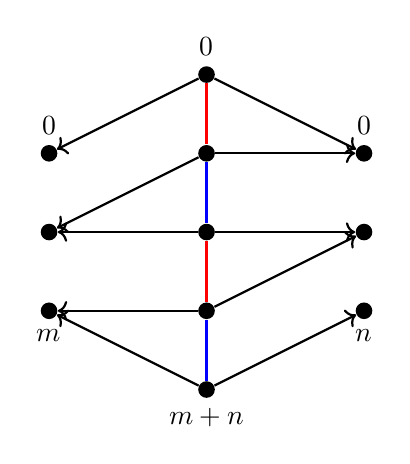
\begin{tikzpicture}[scale=1, transform shape]
            \node[label={north:{$0$}}, fill=black, circle,inner sep=0, minimum size=6pt] (a0) at (0,2) {};
            \node[label={south:{$m+n$}}, fill=black, circle,inner sep=0, minimum size=6pt] (a4) at (0,-2) {};
            \node[fill=black, circle, inner sep=0, minimum size=6pt] (a1) at (0,1) {};
            \node[fill=black, circle, inner sep=0, minimum size=6pt] (a2) at (0,0) {};
            \node[fill=black, circle, inner sep=0, minimum size=6pt] (a3) at (0,-1) {};
            \node[label={north:{$0$}}, fill=black, circle,inner sep=0, minimum size=6pt] (b0) at (-2,1) {};
            \node[label={south:{$m$}}, fill=black, circle,inner sep=0, minimum size=6pt] (b2) at (-2,-1) {};
            \node[fill=black, circle, inner sep=0, minimum size=6pt] (b1) at (-2,0) {};
            \node[label={north:{$0$}}, fill=black, circle,inner sep=0, minimum size=6pt] (c0) at (2,1) {};
            \node[label={south:{$n$}}, fill=black, circle,inner sep=0, minimum size=6pt] (c2) at (2,-1) {};
            \node[fill=black, circle, inner sep=0, minimum size=6pt] (c1) at (2,0) {};
            \draw[thick,->] (a0) -- (b0);
            \draw[thick,->] (a1) -- (b1);
            \draw[thick,->] (a3) -- (b2);
            \draw[thick,->] (a2) -- (b1);
            \draw[thick,->] (a4) -- (b2);
            \draw[thick,->] (a0) -- (c0);
            \draw[thick,->] (a1) -- (c0);
            \draw[thick,->] (a2) -- (c1);
            \draw[thick,->] (a3) -- (c1);
            \draw[thick,->] (a4) -- (c2);
            \draw[thick, red] (a0) -- (a1);
            \draw[thick, red] (a2) -- (a3);
            \draw[thick, blue] (a1) -- (a2);
            \draw[thick, blue] (a3) -- (a4);
        \end{tikzpicture}
        \end{center}
        \caption{A $(2,2)$ shuffle. Red lines denote where $\mu$ jumps and blue lines denote where $\nu$ jumps.}%
        \label{fig:22shuffle}
        \end{figure}
        We can see that an $(m,n)$-shuffle is simply a way to shuffle $m$ red and $n$ blue cards together. There is a unique permutation which takes the configuration having all red cards on top to our given shuffle.
    \end{itemize}
\end{defn}

\begin{prop}
    Let $R \in \ms{scRing}$. Then there is a map \(R_m \otimes R_n \xrightarrow{\cdot} R_{m+n}\) given by the formula
    \[ x \cdot y = \sum_{(\mu, \nu)} \on{sign}(\mu, \nu) s_{\mu}(x) s_{\nu}(y), \]
    where \(s_{\mu}(x)\) and \(s_{\nu}(y)\) correspond to applying the degeneracies making up $\mu$ and $\nu$ to obtain elements of $R_{m+n}$. This gives $R$ the structure of a strict cdga.
\end{prop}

\begin{proof}
    We will not go through all of the combinatorics explicitly.
    \begin{itemize}
        \item To prove associativity, we can express both \((xy)z\) and \(x(yz)\) as a sum
        \[ \sum_{(\lambda,\mu, \nu)}\on{sign}(\lambda, \mu, \nu) s_{\lambda}(x) s_{\mu}(y) s_{\nu}(z). \]
        \item To check commutativity, the fact that $R$ was a simplicial commutative ring means we can exchange the roles of $\mu$ and $\nu$ up to 
        \[ \frac{\on{sign}(\mu, \nu)}{\on{sign}(\nu, \mu)} = (-1)^{mn}, \]
        which is exactly what we desire.
        \item A variant of this argument also gives strictness. When we compute $x^2$, the summands corresponding to $(\mu, \nu)$ and $(\nu, \mu)$ appear with opposite signs, so we see that $x^2 = 0$.
        \item The differential is given by the alternating sum of the face maps. Applying this to $x \cdot y$ will decompose the result into $(m-1, n)$-shuffles and $(m, n-1)$-shuffles, which yields the desired result. \qedhere
    \end{itemize}
\end{proof}

We will now discuss divided power structures. In fact, every simplicial commutative ring will give us one of these.

\begin{prop}
    Let $R \in \ms{scRing}$ be a simplicial commutative ring. Then there exist maps $\gamma_k \colon R_n \to R_{nk}$ for all $n, k \geq 1$ such that
    \begin{itemize}
        \item We have $\gamma_1(x) = x$ for all $x \in R$;
        \item We also have 
        \[ \gamma_k(x) \gamma_{\ell}(x) = \binom{k+\ell}{\ell} \gamma_{k+\ell}(x) \] 
        for all $k, \ell$. This means that we should think that $x^k = k! \gamma_k(x)$;
        \item For all $x,y \in R_n$, we have
        \[ \gamma_k(x+y) = \sum_{i+k=k} \gamma_i(x) \gamma_j(y); \]
        \item Similarly, we have
        \[ \gamma_k(xy) = x^k \gamma_k(y); \]
        \item We have the identity
        \[ \gamma_k (\gamma_{\ell}(x)) = \frac{(k\ell)!}{k! (\ell!)^k} \gamma_{k\ell}(x). \]
    \end{itemize}
\end{prop}

\begin{proof}
    If $x$ is odd, we define $\gamma_1(x) = x$ and $\gamma_k(x) = 0$ for all $k \geq 2$. This is fine because $x^2 = 0$ already. If $x$ is even, we have
    \[ x^k = \sum_{(\mu_1, \ldots, \mu_k)} \on{sign}(\mu_1, \ldots, \mu_k) s_{\mu_1}(x) \cdots s_{\mu_k}(x). \]
    We can permute the factors $\mu_1, \ldots, \mu_k$ (all of the signs will become $+1$), and therefore for all $\sigma \in \Sigma_k$, $(\mu_1, \ldots, \mu_k)$ and $(\mu_{\sigma(1)}, \ldots, \mu_{\sigma(k)})$ give the same summand. Choosing one element from each equivalent class, we obtain an element $\gamma_k(x)$ such that $x^k = k! \gamma_k(x)$.

    We will omit checking that the properties are satisfied.
\end{proof}

We now need to make sure that this divided power structure behaves well with respect to the chain differential.
\begin{prop}
    Let $R \in \ms{scRing}$ be a simplicial commutative ring. Then
    \begin{itemize}
        \item If $x$ is even, then $\d{\gamma_k(x)} = \gamma_{k-1}(x)\cdot \d{x}$;
        \item The maps $\gamma_k$ preserve boundaries;
        \item The $\gamma_k$ give a well-defined divided power structure on $H_*(R)$.
    \end{itemize}
\end{prop}

\begin{proof}
    Suppose that $x$ is a boundary. Then $x = \d{y}$ for $x$ with $\d_i y = 0$ for all $i > 0$. Define
    \[
        \gamma_k'(y) \coloneqq \sum_{\substack{(\mu_1, \ldots, \mu_k) \\ \Sigma_k \text{-representatives}}} \on{sign}(\mu_1, \ldots, \mu_k) s_{\mu_1'}(y) \cdots s_{\mu_k'}(y).
    \]
    Here, for maps $\mu_i \colon [kn] \to [n]$, we set $\mu_i' \colon [1+kn] \to [1+n]$ to be the maps given by sticking a $1$ in front. Then $\d_0 \gamma_k'(y) = \gamma_k(x)$ and $\d_i \gamma_k'(y) = 0$ for all $i > 0$, and therefore $\d{\gamma_k'(y)} = \gamma_k(x)$.
\end{proof}

\section{Cotangent complexes and obstruction theory}%
\label{sec:Cotangent complexes}

\subsection{Definition of the cotangent complex}%
\label{sub:Definition of the cotangent complex}

Recall that we defined
\[ L \Omega^1_{-/k} \colon \ms{Ani}(k\ms{-alg}) \to \mc{D}(\Z)_{\geq 0} \] as the nonabelian derived functor of
\[ \Omega^1 \colon k\ms{-alg} \to \ms{Ab}. \]

\begin{lem}
    The following constructions agree:
    \begin{enumerate}
        \item The functor 
        \[ L \Omega^1_{-/k} \colon \ms{Ani}(k\ms{-alg}) \to \mc{D}(\Z)_{\geq 0} \] evaluated on $R$;
        \item The functor 
        \[ L (A \mapsto R \otimes_A \Omega^1_{A/k}) \colon \ms{Ani}(k\ms{-alg}_{/R}) \to \mc{D}(R)_{\geq 0} \]
        evaluated on $R$.
    \end{enumerate}
\end{lem}

\begin{proof}
    If we begin with the second construction, we obtain
    \begin{align*}
        \colim_{i \in \Delta^{\op}} R \otimes_{A_i}\Omega^1_{A_i/k} &\simeq \colim_{i \in \Delta^{\op}} \ab(\colim_{j \in \Delta^{\op}} A_j) \otimes^{\L}_{A_i} \Omega^1_{A_i/k} \\
        &\simeq \colim_{i \in \Delta^{\op}} \ab(\colim_{j \in \Delta^{\op}_{i/}} A_j) \otimes_{A_i}^{\L} \Omega^1_{A_i/k} \\
        &\simeq \colim_{i \to j \in (\Delta^{\op})^{\Delta^1}} A_j \otimes_{A_i}^{\L} \Omega^1_{A_i/k} \\
        &\simeq \colim_{i \in \Delta^{\op}} \Omega^1_{A_i/k} \\
        &\simeq L \Omega^1_{R/k}.
    \end{align*}
    with $A_i$ polynomial rings. Here, we have used the fact that identity morphisms are cofinal in the arrow category.
\end{proof}

The second functor has better categorical properties than the first. Namely, it commutes with coproducts. By definition, this implies that it preserves all colimits.

\begin{exm}
    If $R = k[x_1, \ldots, x_n] / (f_1, \ldots, f_m)$ is defined by a regular sequence, then the diagram
    \begin{equation*}
    \begin{tikzcd}
        k[f_1, \ldots, f_m] \ar{r} \ar{d} & k[x_1, \ldots, x_m] \ar{d} \\
        k \ar{r} & R
    \end{tikzcd}
    \end{equation*}
    is a pushout in $\ms{Ani}(k\ms{-alg}_{/R})$. The functor $L(R \otimes_{\bullet} \Omega^1_{\bullet/k})$ takes this to
    \begin{equation*}
    \begin{tikzcd}
        R\ab\{\d{f_1}, \ldots, \d{f_m} \}  \ar{r} \ar{d} & R \ab\{ \d{x_1}, \ldots, \d{x_n}\} \ar{d} \\
         0 \ar{r} & L \Omega^1_{R/k},
    \end{tikzcd}
    \end{equation*}
    where the top arrow is the Jacobian matrix of $f_1, \ldots, f_m$. This is also a pushout in $\mc{D}(R)_{\geq 0}$, and therefore $L\Omega^1_{R/k}$ has as $H_0$ and $H_1$ the cokernel and kernel of the Jacobian matrix.
\end{exm}

\begin{defn}
    We will call $\Omega^1_{R/k}$ the \textit{cotangent complex} of $R$ relative to $k$ and denote it by $L_{R/k}$.
\end{defn}

\subsection{Applications to obstruction theory of rings}%
\label{sub:Applications to obstruction theory of rings}

Let $S$ be a ring and $M$ be an $S$-module. We can form a \textit{split square-zero extension} on the $S$-module $S \oplus M$ where
\begin{itemize}
    \item If $m_1, m_2 \in M$, we have $m_1 m_2 = 0$;
    \item Elements of $s$ multiply as usual;
    \item If $s \in S$ and $m \in M$, then $sm$ is given by the usual action of $s$ on $M$.
\end{itemize}
We would like to understand when there is a lift in the diagram
\begin{equation*}
\begin{tikzcd}
    & S \oplus M \ar{d} \\
    R \ar{r}{\varphi} \ar[dashrightarrow]{ur} & S.
\end{tikzcd}
\end{equation*}
These lifts correspond to $\varphi$-linear derivations $R \to M$, which are simply $R$-module maps
\[ \Omega^1_{R/k} \to \varphi_* M. \]

\begin{prop}
    There exists a functor
    \[ \mc{D}(S)_{\geq 0} \to \ms{Ani}(k\ms{-alg})/S \]
    which sends a projective module $P$ to the square-zero extension $S \oplus P$. We have equivalences of mapping spaces
    \[ \ms{Map}_{\mc{D}(R)_{\geq 0}} (L_{R/k}, \varphi_* M) \simeq \on{Fiber} \ab(\begin{matrix}\ms{Map}_{\ms{Ani}(k\ms{-alg})}(R, S \oplus M) \\ \downarrow \\ \ms{Map}_{\ms{Ani}(k\ms{-alg})}(R,S)\end{matrix}). \]
\end{prop}

We would now like to apply this to study ordinary rings. Given a surjective $\tilde{R} \to R$ whose kernel $I$ satisfies $I^2 = 0$, we will call this a \textit{(not necessarily split) square-zero extension}. One example of a non-split square-zero extension is
\[ \Z/p^2 \to \Z/p, \]
which does not even split as a morphism of abelian groups. Note that the condition that $I^2 = 0$ implies that the $\tilde{R}$-action on $I$ factors through $R$.

It turns out that $L_{R/\tilde{R}}$ has $H_0 = 0$ and 
\[ H_1 = R \otimes_{\tilde{R}} I = I. \]
There is a tautological morphism
\[ L_{R/\tilde{R}} \to I[1] \]
of $R$-modules which induces an isomorphism on $H_1$. This corresponds to a map
\[ \delta \colon R \to R \oplus I[1] \]
of animated $\tilde{R}$-algebras.

\begin{prop}
    $\tilde{R}$ is the pullback of the diagram
    \begin{equation*}
    \begin{tikzcd}
        \tilde{R} \ar{r} \ar{d} & R \ar{d}{s} \\
        R \ar{r}{\delta} & R \oplus I[1]
    \end{tikzcd}
    \end{equation*}
    in the category of animated $\tilde{R}$-algebras.
\end{prop}

We see that (not necessarily split) square-zero extensions $\tilde{R} \to R$ along $I$ correspond to maps
\[ L_{R/k} \to I[1]. \]
Maps $S \to \tilde{R}$ lifting a given $S \to R$ correspond to diagrams of the form
\begin{equation*}
\begin{tikzcd}
    & \tilde{R} \ar{r} \ar{d} & R \ar{d}{s} \\
    S \ar[dashrightarrow]{ur} \ar[dashrightarrow]{urr} \ar{r} & R \ar{r}{\delta} & R \oplus I[1],
\end{tikzcd}
\end{equation*}
which are simply lifts
\begin{equation*}
\begin{tikzcd}
    & R \ar{d}{s} \ar[bend left=60]{dd}{\mr{Id}} \\
    S \ar[dashrightarrow,""{swap,name=L}]{ur} \ar{r} & R \oplus I[1] \ar{d} \ar[Leftarrow, to=L] \\
    & R.
\end{tikzcd}
\end{equation*}
If we unwrap everything, we see that a lift exists if and only if the map
\[ L_{S/k} \to I[1] \]
is nullhomotopic. Furthermore, lifts are in correspondence to choices of nullhomotopies. These form a torsor over $\pi_1(\ms{Map}(L_{S/k}, I[1]))$. We therefore see that
\begin{itemize}
    \item The possible square-zero extensions $\tilde{R}$ are classified by
    \[ \pi_0 \ms{Map}_{\mc{D}(R)} (L_{R/k}, I[1]); \]
    \item For a given $\tilde{R}$ and $S \to R$, there is an obstruction living in
    \[ \pi_0 \ms{Map}_{\mc{D}(S)} (L_{S/k}, I[1]). \]
    \item If lifts do exist, they are parameterized by
    \[ \pi_1 \ms{Map}_{\mc{D}(S)} (L_{S/k}, I[1]) \simeq \pi_0 \ms{Map}_{\mc{D}(S)}(L_{S/k}, I). \]
\end{itemize}

\begin{exer}
    Let $S$ be a $k$-algebra. Show that the following are equivalent:
    \begin{enumerate}
        \item For every square-zero extension $\tilde{R} \to R$ and every $S \to R$, there is a lift (this is usually called being \textit{formally smooth}).
        \item We have $H_1(L_{S/k})= 0$ and $H_0(L_{S/k})$ is a projective $S$-module.
    \end{enumerate}
\end{exer}

We are now ready to apply this machinery.
\begin{thm}\label{thm:wittvectors}
    If $R_1$ is a perfect $\F_p$-algebra (this means that Frobenius is an automorphism), then there exist flat $\Z/p^n$-algebras $R_n$, unique up to isomorphism, with 
    \[ R_1 \simeq R_n \otimes_{\Z/p^n} \F_p. \]
    In particular, we have
    \[ R_{n-1} \cong R_n \otimes_{\Z/p^n} \Z/p^{n-1}, \]
    so we have a tower
    \[ \cdots \to R_n \to R_{n-1} \to \cdots \]
    whose lift
    \[ R \coloneqq \lim R_n \]
    is the unique flat, $p$-complete $\Z_p$-algebra satisfying
    \[ R_1 \cong R \otimes_{\Z_p} \F_p. \]
\end{thm}

This theorem tells us that there is a way to escape from the positive characteristic to the mixed characteristic setting under the assumption that $R_1$ is perfect.

We will characterize $R_n$ as a non-split square-zero extension of $R_{n-1}$ by $R_1$. This is because if it exists, tensoring
\[ 0 \to \Z/p \to \Z/p^n \to \Z/p^{n-1} \to 0 \]
with $R_n$ gives us
\[ 0 \to R_1 \to R_n \to R_{n-1} \to 0. \]
These extensions are classified by
\[ \pi_0 \ms{Map}_{\mc{D}(R_{n-1})} (L_{R_{n-1}/\Z}, R_1 [1]). \]
They also need to be compatible with the element of
\[ \pi_0 \ms{Map}_{\mc{D}(\Z/p^{n-1})}(L_{(\Z/p^{n-1})/\Z}, \Z/p[1]) \]
classifying $\Z/p^n \to \Z/p^{n-1}$.

\begin{lem}
    Isomorphism classes of such $R_n$ form a torsor over
    \[ \pi_0 \ms{Map}_{\mc{D}(R_{n-1})} (L_{R_{n-1}/\Z/p^{n-1}}, R_n[1]) \simeq \pi_0 \ms{Map}_{\mc{D}(R_1)} (L_{R_1/\F_p}, R_1[1]). \]
\end{lem}

\begin{lem}
    If $R_1$ is a perfect $\F_p$-algebra, then $L_{R_1/\F_p} \simeq 0$.
\end{lem}

\begin{proof}
    For any perfect $\F_p$-algebra $A$, we will consider the effect of the Frobenius $\varphi \colon A \to A$ on the contangent complex. This induces the zero morphism on $\Omega^1_{A/\F_p}$ (in particular for polynomial rings). Therefore, if we resolve $R_1$ by polynomial rings, $\varphi$ acts by $0$ on $L_{R_1/\F_p}$. However, because we assumed that $R_1$ is perfect, it must also act by an isomorphism. The desired result follows immediately.
\end{proof}

Putting together the two lemmas, we see that there is a unique isomorphism class of possible $R_n$, which proves~\Cref{thm:wittvectors}.

\begin{defn}
    The $R$ in~\Cref{thm:wittvectors} is called the \textit{Witt vectors} of $R$ and denoted by $W(R_0)$.
\end{defn}

\begin{rmk}
    Usually the Witt vectors are given by an explicit construction and exist for any $\F_p$-algebra, not just perfect ones, but we believe this explanation is much more satisfying.
\end{rmk}

\begin{exm}
    Consider the finite field $\F_{p^n}$. The Witt vectors $W(\F_{p^n})$
    is a $\Z_p$-algebra with 
    \[ W(\F_{p^n}) / p \simeq \F_{p^n}. \] 
    One way to construct this is to consider $\F_{p^n} = \F_p[x]/f(x)$ and take the ring
    \[ \Z_p[x]/\tilde{f}(x) \]
    for some lift $\tilde{f}$ of $f$.
\end{exm}


\end{document}